%&preformat-disser
\RequirePackage[l2tabu,orthodox]{nag} % Раскомментировав, можно в логе получать рекомендации относительно правильного использования пакетов и предупреждения об устаревших и нерекомендуемых пакетах
% Формат А4, 14pt (ГОСТ Р 7.0.11-2011, 5.3.6)
\documentclass[a4paper,14pt,oneside,openany]{memoir}

%%%%%%%%%%%%%%%%%%%%%%%%%%%%%%%%%%%%%%%%%%%%%%%%%%%%%%%%%%%%%%%%%%%%%%%%%%%%%%%%
%%%% Файл упрощённых настроек шаблона, общих для диссертации и автореферата %%%%
%%%%%%%%%%%%%%%%%%%%%%%%%%%%%%%%%%%%%%%%%%%%%%%%%%%%%%%%%%%%%%%%%%%%%%%%%%%%%%%%

%%% Режим черновика %%%
\makeatletter
\@ifundefined{c@draft}{
  \newcounter{draft}
  \setcounter{draft}{0}  % 0 --- чистовик (максимальное соблюдение ГОСТ)
                         % 1 --- черновик (отклонения от ГОСТ, но быстрая
                         %       сборка итоговых PDF)
}{}
\makeatother

%%% Пометки в тексте %%%
\makeatletter
\@ifundefined{c@showmarkup}{
  \newcounter{showmarkup}
  \setcounter{showmarkup}{0}  % 0 --- скрыть пометки
                              % 1 --- показывать пометки
}{}
\makeatother

%%% Использование в pdflatex шрифтов не по-умолчанию %%%
\makeatletter
\@ifundefined{c@usealtfont}{
  \newcounter{usealtfont}
  \setcounter{usealtfont}{1}    % 0 --- шрифты на базе Computer Modern
                                % 1 --- использовать пакет pscyr, при его
                                %       наличии
                                % 2 --- использовать пакет XCharter, при наличии
                                %       подходящей версии
}{}
\makeatother

%%% Использование в xelatex и lualatex семейств шрифтов %%%
\makeatletter
\@ifundefined{c@fontfamily}{
  \newcounter{fontfamily}
  \setcounter{fontfamily}{0}  % 0 --- CMU семейство. Используется как fallback;
                              % 1 --- Шрифты от MS (Times New Roman и компания)
                              % 2 --- Семейство Liberation
}{}
\makeatother

%%% Библиография %%%
\makeatletter
\@ifundefined{c@bibliosel}{
  \newcounter{bibliosel}
  \setcounter{bibliosel}{1}   % 0 --- встроенная реализация с загрузкой файла
                              %       через движок bibtex8;
                              % 1 --- реализация пакетом biblatex через движок
                              %       biber
}{}
\makeatother

%%% Вывод типов ссылок в библиографии %%%
\makeatletter
\@ifundefined{c@mediadisplay}{
  \newcounter{mediadisplay}
  \setcounter{mediadisplay}{1}   % 0 --- не делать ничего; надписи [Текст] и
                                 %       [Эл. ресурс] будут выводиться только в ссылках с
                                 %       заполненным полем `media`;
                                 % 1 --- автоматически добавлять надпись [Текст] к ссылкам с
                                 %       незаполненным полем `media`; таким образом, у всех
                                 %       источников будет указан тип, что соответствует
                                 %       требованиям ГОСТ
                                 % 2 --- автоматически удалять надписи [Текст], [Эл. Ресурс] и др.;
                                 %       не соответствует ГОСТ
                                 % 3 --- автоматически удалять надпись [Текст];
                                 %       не соответствует ГОСТ
                                 % 4 --- автоматически удалять надпись [Эл. Ресурс];
                                 %       не соответствует ГОСТ
}{}
\makeatother

%%% Предкомпиляция tikz рисунков для ускорения работы %%%
\makeatletter
\@ifundefined{c@imgprecompile}{
  \newcounter{imgprecompile}
  \setcounter{imgprecompile}{0}   % 0 --- без предкомпиляции;
                                  % 1 --- пользоваться предварительно
                                  %       скомпилированными pdf вместо генерации
                                  %       заново из tikz
}{}
\makeatother
            % общие настройки шаблона
\input{common/packages}         % Пакеты общие для диссертации и автореферата
\synopsisfalse                      % Этот документ --- не автореферат
\input{Dissertation/dispackages}    % Пакеты для диссертации
\input{Dissertation/userpackages}   % Пакеты для специфических пользовательских задач

%%%%%%%%%%%%%%%%%%%%%%%%%%%%%%%%%%%%%%%%%%%%%%%%%%%%%%
%%%% Файл упрощённых настроек шаблона диссертации %%%%
%%%%%%%%%%%%%%%%%%%%%%%%%%%%%%%%%%%%%%%%%%%%%%%%%%%%%%

%%% Инициализирование переменных, не трогать!  %%%
\newcounter{intvl}
\newcounter{otstup}
\newcounter{contnumeq}
\newcounter{contnumfig}
\newcounter{contnumtab}
\newcounter{pgnum}
\newcounter{chapstyle}
\newcounter{headingdelim}
\newcounter{headingalign}
\newcounter{headingsize}
%%%%%%%%%%%%%%%%%%%%%%%%%%%%%%%%%%%%%%%%%%%%%%%%%%%%%%

%%% Область упрощённого управления оформлением %%%

%% Интервал между заголовками и между заголовком и текстом %%
% Заголовки отделяют от текста сверху и снизу
% тремя интервалами (ГОСТ Р 7.0.11-2011, 5.3.5)
\setcounter{intvl}{3}               % Коэффициент кратности к размеру шрифта

%% Отступы у заголовков в тексте %%
\setcounter{otstup}{0}              % 0 --- без отступа; 1 --- абзацный отступ

%% Нумерация формул, таблиц и рисунков %%
% Нумерация формул
\setcounter{contnumeq}{0}   % 0 --- пораздельно (во введении подряд,
                            %       без номера раздела);
                            % 1 --- сквозная нумерация по всей диссертации
% Нумерация рисунков
\setcounter{contnumfig}{0}  % 0 --- пораздельно (во введении подряд,
                            %       без номера раздела);
                            % 1 --- сквозная нумерация по всей диссертации
% Нумерация таблиц
\setcounter{contnumtab}{1}  % 0 --- пораздельно (во введении подряд,
                            %       без номера раздела);
                            % 1 --- сквозная нумерация по всей диссертации

%% Оглавление %%
\setcounter{pgnum}{1}       % 0 --- номера страниц никак не обозначены;
                            % 1 --- Стр. над номерами страниц (дважды
                            %       компилировать после изменения настройки)
\settocdepth{subsection}    % до какого уровня подразделов выносить в оглавление
\setsecnumdepth{subsection} % до какого уровня нумеровать подразделы


%% Текст и форматирование заголовков %%
\setcounter{chapstyle}{1}     % 0 --- разделы только под номером;
                              % 1 --- разделы с названием "Глава" перед номером
\setcounter{headingdelim}{1}  % 0 --- номер отделен пропуском в 1em или \quad;
                              % 1 --- номера разделов и приложений отделены
                              %       точкой с пробелом, подразделы пропуском
                              %       без точки;
                              % 2 --- номера разделов, подразделов и приложений
                              %       отделены точкой с пробелом.

%% Выравнивание заголовков в тексте %%
\setcounter{headingalign}{0}  % 0 --- по центру;
                              % 1 --- по левому краю

%% Размеры заголовков в тексте %%
\setcounter{headingsize}{0}   % 0 --- по ГОСТ, все всегда 14 пт;
                              % 1 --- пропорционально изменяющийся размер
                              %       в зависимости от базового шрифта

%% Подпись таблиц %%

% Смещение строк подписи после первой строки
\newcommand{\tabindent}{0cm}

% Тип форматирования заголовка таблицы:
% plain --- название и текст в одной строке
% split --- название и текст в разных строках
\newcommand{\tabformat}{plain}

%%% Настройки форматирования таблицы `plain`

% Выравнивание по центру подписи, состоящей из одной строки:
% true  --- выравнивать
% false --- не выравнивать
\newcommand{\tabsinglecenter}{false}

% Выравнивание подписи таблиц:
% justified   --- выравнивать как обычный текст («по ширине»)
% centering   --- выравнивать по центру
% centerlast  --- выравнивать по центру только последнюю строку
% centerfirst --- выравнивать по центру только первую строку (не рекомендуется)
% raggedleft  --- выравнивать по правому краю
% raggedright --- выравнивать по левому краю
\newcommand{\tabjust}{justified}

% Разделитель записи «Таблица #» и названия таблицы
\newcommand{\tablabelsep}{~\cyrdash\ }

%%% Настройки форматирования таблицы `split`

% Положение названия таблицы:
% \centering   --- выравнивать по центру
% \raggedleft  --- выравнивать по правому краю
% \raggedright --- выравнивать по левому краю
\newcommand{\splitformatlabel}{\raggedleft}

% Положение текста подписи:
% \centering   --- выравнивать по центру
% \raggedleft  --- выравнивать по правому краю
% \raggedright --- выравнивать по левому краю
\newcommand{\splitformattext}{\raggedright}

%% Подпись рисунков %%
%Разделитель записи «Рисунок #» и названия рисунка
\newcommand{\figlabelsep}{~\cyrdash\ }  % (ГОСТ 2.105, 4.3.1)
                                        % "--- здесь не работает

%%% Цвета гиперссылок %%%
% Latex color definitions: http://latexcolor.com/
\definecolor{linkcolor}{rgb}{0.9,0,0}
\definecolor{citecolor}{rgb}{0,0.6,0}
\definecolor{urlcolor}{rgb}{0,0,1}
%\definecolor{linkcolor}{rgb}{0,0,0} %black
%\definecolor{citecolor}{rgb}{0,0,0} %black
%\definecolor{urlcolor}{rgb}{0,0,0} %black

%                                 ________________________
% ______________________________/ User-defined glossaries

\usepackage[acronym,nopostdot,nonumberlist]{glossaries}
% nopostdot -- do not use dot after the article
% nonumberlist -- do not print list of pages
%
% Custom Glossary Style {{{
\newglossarystyle{plainemdash}{
  \setglossarystyle{list}
  \renewenvironment{theglossary}
    {\begin{list}{}{\setlength{\leftmargin}{0pt}
                    \setlength{\labelwidth}{0pt}
                    \setlength{\itemindent}{6.75pt}
                    \setlength{\listparindent}{0pt}
                    \setlength{\parsep}{\parskip}}}
    {\end{list}}
    \renewcommand*{\glossentry}[2]{%
        \item[\glsentryitem{##1}\glstarget{##1}{\textbf{\glossentryname{##1}}}]%
        ---\ %
        \glossentrydesc{##1}%
        \unskip\leaders\hbox to 2.9mm{\hss.}\hfill##2}%
}
\makeglossaries
\newacronym{dbms}{СУБД}{Система управления базами данных}
\newacronym{db}{БД}{База данных}
\newacronym{hep}{ФВЭ}{Физика высоких энергий}
\newacronym{lms}{МНК}{Метод наименьших квадратов}
\newacronym{oop}{ООП}{Объектно-ориентированное программирование}
\newacronym{dsl}{ПОЯ}{Предметно-ориентированный язык программирования}
\newacronym{sw}{ПО}{Программное обеспечение}
\newacronym{api}{API}{\emph{англ.} Application program interface, программный интерфейс приложения}
\newacronym{fpga}{ПЛИС}{Программируемая логическая интегральная схема}
\newacronym{sfinae}{SFINAE}{Substitution failure is not an error}
\newacronym{crtp}{CRTP}{Curiously recurring template pattern}
\newacronym{fdd}{FDD}{Feature-driven development}
\newacronym{ddd}{DDD}{Domain-driven development}
\newacronym{htc}{HTC}{High throughput computing}
\newacronym{hpc}{HPC}{High performance computing}
\newacronym{mc}{МК}{методы моделирования Монте-Карло}

\newacronym{adc}{АЦП}{Аналогово-цифровой преобразователь}
\newacronym{sadc}{САЦП}{Сэмплирующий аналогово-цифровой преобразователь}
\newacronym{tdc}{ВЦП}{Время-цифровой преобразователь}
\newacronym{pmt}{ФЭУ}{Фотоэлектронный умножитель}
\newacronym{pmma}{ПММА}{Полиметилметакрилат}

\newacronym{sm}{СМ}{Стандартная модель}
\newacronym{mip}{MIP}{Minimum ionizing particle, минимально-ионизирующая частица}
\newacronym{dm}{ТМ}{Тёмная материя}
\newacronym{daf}{DAF}{\emph{англ.} Deterministic annealing filter}
\newacronym{krf}{KRF}{Kalman filter with reference track}

\newacronym{sle}{СЛАУ}{Система линейных уравнений}

\newglossaryentry{serialization}
{
    name=сериализация,
    description={представление экземпляра составного типа данных в виде
    байтовой последовательности, используемое для хранения или
    передачи данных по сетевым протоколам, используемое с целью последующего
    восстановления экземпляра второй стороной (десереализации)},
    %
    user1=сериализации, % родительный, (нет) кого, чего?
    user2=сериализации, % дательный (дам) кому? чему?
    user3=сериализацию, % винительный (вижу) кого? что?
    user4=сериализацией, % творительный (доволен) кем? чем?
    user5=сериализации, % предложный (думаю) о ком? о чём?
}

\newglossaryentry{deserialization}
{
    name=десериализация,
    description={восстановление экземпляра составного типа данных из
    байтовой последовательности},
    user1=десериализации, % родительный, (нет) кого, чего?
    user2=десериализации, % дательный (дам) кому? чему?
    user3=десериализацию, % винительный (вижу) кого? что?
    user4=десериализацией, % творительный (доволен) кем? чем?
    user5=десериализации, % предложный (думаю) о ком? о чём?
}

\newglossaryentry{allocator}
{
    name=аллокатор,
    description={объект управляющий динамическим выделением и освобождением памяти},
    user1=аллокатора, % родительный, (нет) кого, чего?
    user2=аллокатору, % дательный (дам) кому? чему?
    user3=аллокатор, % винительный (вижу) кого? что?
    user4=аллокатором, % творительный (доволен) кем? чем?
    user5=аллокаторе, % предложный (думаю) о ком? о чём?
}

\newglossaryentry{metaprogramming}{
    name=метапрограммирование,
    description={подход к разработке программного обеспечения, при
    котором создаются программы способные генерировать или преобразовывать
    другие программы (в том числе самих себя) как данные},
    user1=метапрограммирования, % родительный, (нет) кого, чего?
    user2=метапрограммированию, % дательный (дам) кому? чему?
    user3=метапрограммирование, % винительный (вижу) кого? что?
    user4=метапрограммированием, % творительный (доволен) кем? чем?
    user5=метапрограммировании, % предложный (думаю) о ком? о чём?
}

\newcommand{\glsgenitive}[1]{\glsuseri{#1}}   % ...... родительный, (нет) кого, чего?
\newcommand{\glsdative}[1]{\glsuserii{#1}}  % ......... дательный (дам) кому? чему?
\newcommand{\glsaccusative}[1]{\glsuseriii{#1}}  % .... винительный (вижу) кого? что?
\newcommand{\glsinstrumental}[1]{\glsuseriv{#1}} % .... творительный(доволен) кем? чем?
\newcommand{\glsprepositional}[1]{\glsuserv{#1}}  % ... предложный (думаю) о ком? о чём?

%    user1=,  % родительный, (нет) кого, чего?
%    user2=,  % дательный (дам) кому? чему?
%    user3=,  % винительный (вижу) кого? что?
%    user4=,  % творительный (доволен) кем? чем?
%    user5=,  % предложный (думаю) о ком? о чём?

%\textbf{TeX} : Cистема компьютерной вёрстки, разработанная американским профессором информатики Дональдом Кнутом
%\textbf{панграмма} : Короткий текст, использующий все или почти все буквы алфавита

      % Упрощённые настройки шаблона

\input{common/newnames}         % Новые переменные, для всего проекта

%%% Основные сведения %%%
\newcommand{\thesisAuthorLastName}{Дусаев}
\newcommand{\thesisAuthorOtherNames}{Ренат Рамильевич}
\newcommand{\thesisAuthorInitials}{Р.\,Р.}
\newcommand{\thesisAuthor}             % Диссертация, ФИО автора
{%
    \texorpdfstring{% \texorpdfstring takes two arguments and uses the first for (La)TeX and the second for pdf
        \thesisAuthorLastName~\thesisAuthorOtherNames% так будет отображаться на титульном листе или в тексте, где будет использоваться переменная
    }{%
        \thesisAuthorLastName, \thesisAuthorOtherNames% эта запись для свойств pdf-файла. В таком виде, если pdf будет обработан программами для сбора библиографических сведений, будет правильно представлена фамилия.
    }
}
\newcommand{\thesisAuthorShort}        % Диссертация, ФИО автора инициалами
{\thesisAuthorInitials~\thesisAuthorLastName}
%\newcommand{\thesisUdk}                % Диссертация, УДК
%{\fixme{xxx.xxx}}
\newcommand{\thesisTitle}              % Диссертация, название
{Программный комплекс для физической реконструкции и анализа событий в экспериментах с триггерной системой}
\newcommand{\thesisSpecialtyNumber}    % Диссертация, специальность, номер
{1.3.2}
\newcommand{\thesisSpecialtyTitle}     % Диссертация, специальность, название (название взято с сайта ВАК для примера)
{Приборы и методы экспериментальной физики}
%% \newcommand{\thesisSpecialtyTwoNumber} % Диссертация, вторая специальность, номер
%% {\fixme{XX.XX.XX}}
%% \newcommand{\thesisSpecialtyTwoTitle}  % Диссертация, вторая специальность, название
%% {\fixme{Теория и~методика физического воспитания, спортивной тренировки,
%% оздоровительной и~адаптивной физической культуры}}
\newcommand{\thesisDegree}             % Диссертация, ученая степень
{кандидата физико-математических наук}
\newcommand{\thesisDegreeShort}        % Диссертация, ученая степень, краткая запись
{канд. физ.-мат. наук}
\newcommand{\thesisCity}               % Диссертация, город написания диссертации
{Томск}
\newcommand{\thesisYear}               % Диссертация, год написания диссертации
{\the\year}
\newcommand{\thesisOrganization}       % Диссертация, организация
{Федеральное государственное автономное образовательное учреждение
высшего образования <<Национальный Исследовательский Томский
политехнический университет>>}
\newcommand{\thesisOrganizationShort}  % Диссертация, краткое название организации для доклада
{НИ ТПУ}

\newcommand{\thesisInOrganization}     % Диссертация, организация в предложном падеже: Работа выполнена в ...
{федеральном государственном автономном образовательном учреждении
высшего образования <<Национальный Исследовательский Томский
политехнический университет>>}

%% \newcommand{\supervisorDead}{}           % Рисовать рамку вокруг фамилии
\newcommand{\supervisorFio}              % Научный руководитель, ФИО
{Любовицкий Валерий Ефимович}
\newcommand{\supervisorRegalia}          % Научный руководитель, регалии
{доктор физ.-мат. наук, профессор}
\newcommand{\supervisorFioShort}         % Научный руководитель, ФИО
{В.\,Е.~Любовицкий}
\newcommand{\supervisorRegaliaShort}     % Научный руководитель, регалии
{д.ф.-м.н., проф.}

%% \newcommand{\supervisorTwoDead}{}        % Рисовать рамку вокруг фамилии
%% \newcommand{\supervisorTwoFio}           % Второй научный руководитель, ФИО
%% {\fixme{Фамилия Имя Отчество}}
%% \newcommand{\supervisorTwoRegalia}       % Второй научный руководитель, регалии
%% {\fixme{уч. степень, уч. звание}}
%% \newcommand{\supervisorTwoFioShort}      % Второй научный руководитель, ФИО
%% {\fixme{И.\,О.~Фамилия}}
%% \newcommand{\supervisorTwoRegaliaShort}  % Второй научный руководитель, регалии
%% {\fixme{уч.~ст.,~уч.~зв.}}

\newcommand{\opponentOneFio}           % Оппонент 1, ФИО
{\fixme{Фамилия Имя Отчество}}
\newcommand{\opponentOneRegalia}       % Оппонент 1, регалии
{\fixme{доктор физико-математических наук, профессор}}
\newcommand{\opponentOneJobPlace}      % Оппонент 1, место работы
{\fixme{Не очень длинное название для места работы}}
\newcommand{\opponentOneJobPost}       % Оппонент 1, должность
{\fixme{старший научный сотрудник}}

\newcommand{\opponentTwoFio}           % Оппонент 2, ФИО
{\fixme{Фамилия Имя Отчество}}
\newcommand{\opponentTwoRegalia}       % Оппонент 2, регалии
{\fixme{кандидат физико-математических наук}}
\newcommand{\opponentTwoJobPlace}      % Оппонент 2, место работы
{\fixme{Основное место работы c длинным длинным длинным длинным названием}}
\newcommand{\opponentTwoJobPost}       % Оппонент 2, должность
{\fixme{старший научный сотрудник}}

%% \newcommand{\opponentThreeFio}         % Оппонент 3, ФИО
%% {\fixme{Фамилия Имя Отчество}}
%% \newcommand{\opponentThreeRegalia}     % Оппонент 3, регалии
%% {\fixme{кандидат физико-математических наук}}
%% \newcommand{\opponentThreeJobPlace}    % Оппонент 3, место работы
%% {\fixme{Основное место работы c длинным длинным длинным длинным названием}}
%% \newcommand{\opponentThreeJobPost}     % Оппонент 3, должность
%% {\fixme{старший научный сотрудник}}

\newcommand{\leadingOrganizationTitle} % Ведущая организация, дополнительные строки. Удалить, чтобы не отображать в автореферате
{\fixme{Ведущая организация <<Ведущая организация>>}}

\newcommand{\defenseDate}              % Защита, дата
{\fixme{DD mmmmmmmm YYYY~г.~в~XX часов}}
\newcommand{\defenseCouncilNumber}     % Защита, номер диссертационного совета
{\fixme{Д\,123.456.78}}
\newcommand{\defenseCouncilTitle}      % Защита, учреждение диссертационного совета
{\fixme{Название учреждения}}
\newcommand{\defenseCouncilAddress}    % Защита, адрес учреждение диссертационного совета
{\fixme{Адрес}}
\newcommand{\defenseCouncilPhone}      % Телефон для справок
{\fixme{+7~(0000)~00-00-00}}

\newcommand{\defenseSecretaryFio}      % Секретарь диссертационного совета, ФИО
{\fixme{Фамилия Имя Отчество}}
\newcommand{\defenseSecretaryRegalia}  % Секретарь диссертационного совета, регалии
{\fixme{д-р~физ.-мат. наук}}            % Для сокращений есть ГОСТы, например: ГОСТ Р 7.0.12-2011 + http://base.garant.ru/179724/#block_30000

\newcommand{\synopsisLibrary}          % Автореферат, название библиотеки
{\fixme{Название библиотеки}}
\newcommand{\synopsisDate}             % Автореферат, дата рассылки
{\fixme{DD mmmmmmmm}\the\year~года}

% To avoid conflict with beamer class use \providecommand
\providecommand{\keywords}%            % Ключевые слова для метаданных PDF диссертации и автореферата
{}
             % Основные сведения
\input{common/fonts}            % Определение шрифтов (частичное)
\input{common/styles}           % Стили общие для диссертации и автореферата
% typewriter font for computer words: tokens, literals, etc.
\newcommand*{\codeword}[1]{\texttt{#1}}
% at some epslatex plots, used to decrease on-plot labels font size
\newcommand{\smllbl}[0]{\tiny}
% Russian areatangent (hyperbolic revert tangent)
%\usepackage{amsmath}
\DeclareMathOperator\arctanh{arth}
% Differential operator
\newcommand*{\diffdchar}{d}    % or {ⅆ}, or {\mathrm{d}}, or whatever standard you’d like to adhere to
\newcommand*{\dd}{\mathop{\diffdchar\!}}
\catcode`\ⅆ=\active
\letⅆ=\dd
% Double tilde
%\usepackage{accents}
\newcommand{\dbtilde}[1]{\accentset{\approx}{#1}}
\newcommand{\vardbtilde}[1]{\tilde{\raisebox{0pt}[0.85\height]{$\tilde{#1}$}}}
% Complex i and exponential
\newcommand{\complexI}[0]{\mathfrak{i}}
\newcommand{\expNum}[0]{\mathfrak{e}}
         % Пользовательские определения
\input{Dissertation/disstyles}  % Стили для диссертации
\input{Dissertation/userstyles} % Стили для специфических пользовательских задач

%%% Библиография. Выбор движка для реализации %%%
% Здесь только проверка установленного ключа. Сама настройка выбора движка
% размещена в common/setup.tex
\ifnumequal{\value{bibliosel}}{0}{%
    \input{biblio/predefined}   % Встроенная реализация с загрузкой файла через движок bibtex8
}{
    \input{biblio/biblatex}     % Реализация пакетом biblatex через движок biber
}

% Вывести информацию о выбранных опциях в лог сборки
\typeout{Selected options:}
\typeout{Draft mode: \arabic{draft}}
\typeout{Font: \arabic{fontfamily}}
\typeout{AltFont: \arabic{usealtfont}}
\typeout{Bibliography backend: \arabic{bibliosel}}
\typeout{Precompile images: \arabic{imgprecompile}}
% Вывести информацию о версиях используемых библиотек в лог сборки
\listfiles

%%% Управление компиляцией отдельных частей диссертации %%%
% Необходимо сначала иметь полностью скомпилированный документ, чтобы все
% промежуточные файлы были в наличии
% Затем, для вывода отдельных частей можно воспользоваться командой \includeonly
% Ниже примеры использования команды:
%
%\includeonly{Dissertation/part2}
%\includeonly{Dissertation/contents,Dissertation/appendix,Dissertation/conclusion}
%
% Если все команды закомментированы, то документ будет выведен в PDF файл полностью

\begin{document}
%%% Переопределение именований типовых разделов
% https://tex.stackexchange.com/a/156050
\gappto\captionsrussian{\input{common/renames}} % for polyglossia and babel
\input{common/renames}
\gappto\captionsrussian{\input{Dissertation/renames}} % for polyglossia and babel
\input{Dissertation/renames}

%%% Структура диссертации (ГОСТ Р 7.0.11-2011, 4)
\thispagestyle{empty}

\noindent%
\begin{tabularx}{\textwidth}{@{}lXr@{}}%
    & & \large{На правах рукописи}\\
    \IfFileExists{images/logo.pdf}{\includegraphics[height=2.5cm]{logo}}{\rule[0pt]{0pt}{1.5cm}}  & &
    \ifnumequal{\value{showperssign}}{0}{%
        \rule[0pt]{0pt}{1.5cm}
    }{
        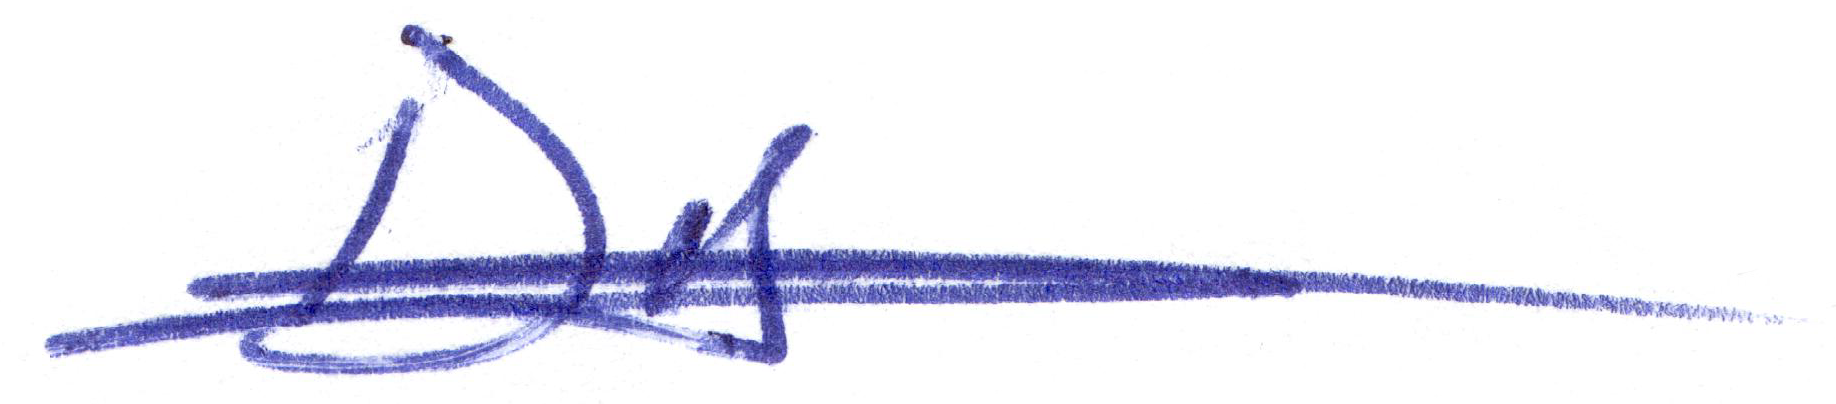
\includegraphics[height=.85cm]{personal-signature.png}
    }\\
\end{tabularx}

\vspace{0pt plus1fill} %число перед fill = кратность относительно некоторого расстояния fill, кусками которого заполнены пустые места
\begin{center}
\textbf {\large \thesisAuthor}
\end{center}

\vspace{0pt plus3fill} %число перед fill = кратность относительно некоторого расстояния fill, кусками которого заполнены пустые места
\begin{center}
\textbf {\Large %\MakeUppercase
\thesisTitle}

\vspace{0pt plus3fill} %число перед fill = кратность относительно некоторого расстояния fill, кусками которого заполнены пустые места
{\large Специальность \thesisSpecialtyNumber\ "---\par <<\thesisSpecialtyTitle>>}

\ifdefined\thesisSpecialtyTwoNumber
{\large Специальность \thesisSpecialtyTwoNumber\ "---\par <<\thesisSpecialtyTwoTitle>>}
\fi

\vspace{0pt plus1.5fill} %число перед fill = кратность относительно некоторого расстояния fill, кусками которого заполнены пустые места
\Large{Автореферат}\par
\large{диссертации на соискание учёной степени\par \thesisDegree}
\end{center}

\vspace{0pt plus4fill} %число перед fill = кратность относительно некоторого расстояния fill, кусками которого заполнены пустые места
{\centering\thesisCity~--- \thesisYear\par}

\newpage
% оборотная сторона обложки
\thispagestyle{empty}
\noindent Работа выполнена в {\thesisInOrganization}.

\vspace{0.008\paperheight plus1fill}
\noindent%
\begin{tabularx}{\textwidth}{@{}lX@{}}
    \ifdefined\supervisorTwoFio
    Научные руководители:   & \supervisorRegalia\par
                              \ifdefined\supervisorDead
                              \framebox{\textbf{\supervisorFio}}
                              \else
                              \textbf{\supervisorFio}
                              \fi
                              \par
                              \vspace{0.013\paperheight}
                              \supervisorRegalia\par
                              \ifdefined\supervisorTwoDead
                              \framebox{\textbf{\supervisorTwoFio}}
                              \else
                              \textbf{\supervisorTwoFio}
                              \fi
                              \vspace{0.013\paperheight}\\
    \else
    Научный руководитель:   & \supervisorRegalia\par
                              \ifdefined\supervisorDead
                              \framebox{\textbf{\supervisorFio}}
                              \else
                              \textbf{\supervisorFio}
                              \fi
                              \vspace{0.013\paperheight}\\
    \fi
    Официальные оппоненты:  &
    \ifnumequal{\value{showopplead}}{0}{\vspace{13\onelineskip plus1fill}}{%
        \textbf{\opponentOneFio,}\par
        \opponentOneRegalia,\par
        \opponentOneJobPlace,\par
        \opponentOneJobPost\par
        \vspace{0.01\paperheight}
        \textbf{\opponentTwoFio,}\par
        \opponentTwoRegalia,\par
        \opponentTwoJobPlace,\par
        \opponentTwoJobPost
    \ifdefined\opponentThreeFio
        \par
        \vspace{0.01\paperheight}
        \textbf{\opponentThreeFio,}\par
        \opponentThreeRegalia,\par
        \opponentThreeJobPlace,\par
        \opponentThreeJobPost
    \fi
    }%
    \vspace{0.013\paperheight} \\
    \ifdefined\leadingOrganizationTitle
    Ведущая организация:    &
    \ifnumequal{\value{showopplead}}{0}{\vspace{6\onelineskip plus1fill}}{%
        \leadingOrganizationTitle
    }%
    \fi
\end{tabularx}
\vspace{0.008\paperheight plus1fill}

\noindent Защита состоится \defenseDate~на~заседании диссертационного совета \defenseCouncilNumber~при \defenseCouncilTitle~по адресу: \defenseCouncilAddress.

\vspace{0.008\paperheight plus1fill}
\noindent С диссертацией можно ознакомиться в библиотеке \synopsisLibrary.

\vspace{0.008\paperheight plus1fill}
\noindent Отзывы на автореферат в двух экземплярах, заверенные печатью учреждения, просьба направлять по адресу: \defenseCouncilAddress, ученому секретарю диссертационного совета~\defenseCouncilNumber.

\vspace{0.008\paperheight plus1fill}
\noindent{Автореферат разослан \synopsisDate.}

\noindent Телефон для справок: \defenseCouncilPhone.

\vspace{0.008\paperheight plus1fill}
\noindent%
\begin{tabularx}{\textwidth}{@{}%
>{\raggedright\arraybackslash}b{18em}@{}
>{\centering\arraybackslash}X
r
@{}}
    Ученый секретарь\par
    диссертационного совета\par
    \defenseCouncilNumber,\par
    \defenseSecretaryRegalia
    &
    \ifnumequal{\value{showsecrsign}}{0}{}{%
        
\includegraphics[width=2cm]{secretary-signature.png}%
    }%
    &
    \defenseSecretaryFio
\end{tabularx}
           % Титульный лист
\include{Dissertation/contents}        % Оглавление
\ifnumequal{\value{contnumfig}}{1}{}{\counterwithout{figure}{chapter}}
\ifnumequal{\value{contnumtab}}{1}{}{\counterwithout{table}{chapter}}
\include{Dissertation/introduction}    % Введение
\ifnumequal{\value{contnumfig}}{1}{\counterwithout{figure}{chapter}
}{\counterwithin{figure}{chapter}}
\ifnumequal{\value{contnumtab}}{1}{\counterwithout{table}{chapter}
}{\counterwithin{table}{chapter}}

\chapter{Методология разработки программного обеспечения}

Возросший в последние десятилетия коммерческий интерес к
различным практикам разработки программного обеспечения
привёл к формированию различных методологий в рамках
корпоративных процессов, с широким охватом различных областей
человеческой деятельности -- от сферы услуг, до специализированных
научных инструментов в рамках инновационных разработок.
Отдельные методики должны быть применимы и в рамках разработки
программного обеспечения для целей автоматизации физического
эксперимента.

Выбор методологии определяет стратегию и последовательность
разработки, набор ключевых понятий и в немалой степени -- архитектуру
программного обеспечения.

%\acrshort{hep}

%В данной главе приведён краткий обзор наиболее популярных в предметной
%области экспериментальной физики частиц программных решений, выделяются
%типовые сценарии использования \acrshort{ПО}, предполагаются и
%обосновываются важные архитектурные решения, формулируются спецификации
%под соответствующие варианты использования программного комплекса.

%В настоящей главе рассматривается методология разработки
%программного обеспечения в контексте общих задач физического эксперимента,
%выделяются общие контексты вариантов использования,
%формулируются требования к архитектуре программного обеспечения
%формулируются принципы построения модульной системы программного комплекса.

\section{Выбор методологии}

%Жизненный цикл научного ПО краток по сравнению с таковым в
%коммерческой разработке: после проведения измерений, проверки гипотез
%и опубликования результатов (то есть, выполнения цели научной
%программы), продукт как целое быстро утрачивает актуальность ввиду
%развития методов измерений, средств анализа и теоретических моделей.
%При этом отдельные компоненты системы могут
%представлять ценность, и должны допускать повторное
%использование (то есть должны быть в достаточной степени изолированы
%и переносимы). Это обуславливает первое важное требование
%к системе -- модульность.
%
%Модульность предполагает не только декомпозицию программы на
%отдельные семантические узлы, но и предусмотренные конкретным
%техническим средством механизмы замены, дополнения или удаления
%модуля без ущерба для работоспособности системы в целом.
Жизненный цикл научного программного обеспечения обычно короче, чем у коммерческих систем~\cite{lifecycle-lenhardt2014data, Przedzinski2020PhD}: после завершения измерений, проверки гипотез и публикации результатов программный продукт в целом быстро теряет актуальность из-за развития методов измерений, анализа и теоретических моделей~\cite{hep-roadmap-Albrecht2019}. Тем не менее отдельные его компоненты сохраняют ценность и потому должны быть изолированными и переносимыми, что выражается в таком качестве системы как \emph{модульность}. Следует подчеркнуть, что под модульностью понимается не только разбиение программы на функциональные блоки, но и предусмотренная конкретными техническими средствами возможность их замены, дополнения или удаления без ущерба для системы в целом.

%В связи с этим целесообразно обратиться к семейству методологий
%т.н. гибкой разработки программного
%обеспечения (Agile)~\cite{AgileManifesto2001}. В рамках этого семейства,
%каждая методология предлагают построить весь процесс в целом, с расчётом на
%изменчивость отдельных компонент.
Учитывая эту специфику, при проектировании целесообразно опираться на методологии гибкой разработки программного обеспечения (Agile)~\cite{AgileManifesto2001}, которые изначально ориентированы на изменчивость требований и компонентов. Такой подход обеспечивает адаптивность и устойчивость программных систем в условиях эволюции исследовательских задач.

%Хотя монолитность не является неотъемлемым свойством
%таких приложений, в отсутствие усилий по проектированию ПО, часто
%приводит к тому что повторное использование решений становится дороже
%их повторной реализации.

\subsection{Гибкие методологии}

Разработка научного программного обеспечения существенно отличается от
коммерческих практик. Во-первых, здесь отсутствует внешний заказчик
и формализованное техническое задание: постановка задачи формируется
самими исследователями в зависимости от актуальных научных
проблем~\cite{software-for-science-CarverEtAl2016}.
Во-вторых, организационная структура научных групп обычно не
предполагает выделенных менеджеров проектов, и ключевую роль играют
специалисты в предметной области, чьи компетенции в области
разработки программ не обязательно включают беглое понимание
общего контекста, перспектив и стратегии разработки.
В-третьих, часто требуется в сжатые сроки получить конкретный
физический результат (требование высокой доступности решения),
что нередко приводит к компромиссам
в части архитектурной строгости и сопровождаемости кода. Наконец,
значительная доля разработок носит характер рабочих прототипов и
имеет крайне короткий жизненный цикл, ограниченный решением
конкретной вычислительной задачи.

Совокупность этих факторов делает традиционные модели разработки
малоприменимыми и усиливает актуальность гибких методологий,
учитывающих изменчивость требований и обеспечивающих
высокую доступность программного решения. В этом контексте
наибольшую релевантность имеют
три направления из семейства Agile: Domain-Driven Development %(\acrshort{ddd})~\cite{vernon-DDD},
(\acrshort{ddd})~\cite{vernon-DDD},
%(DDD)~\cite{vernon-DDD} \nomenclature{DDD}{Domain-Driven Development\nomrefpage}
обеспечивающее формализацию понятийного аппарата предметной
области; Feature-Driven Development \acrshort{fdd},~\cite{coad1999java-fdd})
%\nomenclature{FDD}{Feature-Driven Development\nomrefpage}
, структурирующее процесс
вокруг реализуемых функций; и Data-Driven Development \cite{Treleaven1982ddd, llopis2009ddd},
ориентированное на построение решений исходя из характера и
динамики обрабатываемых данных.

\begin{comment}
\begin{itemize}
    \item Предметно-ориентированное проектирование
    (<<\emph{Domain Driven Development}>>, \acrshort{ddd})~\cite{vernon-DDD}
    %опирается на глубокое понимание .
    %Согласно этим принципам,
    в рамках которой информационная система проектируется так чтобы
    элементы архитектуры \acrshort{sw} отвечали естественной
    понятийной базе принятой в предметной области, включая специальную
    терминологию, бизнес-логику и т.д.
    \item Разработка управляемая функциями \acrshort{sw} (<<\emph{Feature Driven Development}>>, \acrshort{fdd},~\cite{coad1999java-fdd}) представляет
    собой итеративную методологию, разделяя конечную функциональность
    продукта на отдельные функции. Важно, что на этапе начального
    проектирования, набор функций неполон, не вполне известен и допускает
    изменение уже реализованных спецификаций до окончания жизненного
    цикла \acrshort{sw}.
    \item Проектирование \acrshort{sw} на основе данных (<<\emph{Data Driven Development}>>, первые принципы формулируются в контексте разработки
    процессорных архитектур в
    работе \cite{Treleaven1982ddd}, современное понимание развивается от
    работы \cite{llopis2009ddd})
    подразумевает проектирование и разработку \acrshort{sw} отвечающего
    конкретным количественным критериям.
\end{itemize}
\end{comment}

Нужно подчеркнуть, что в подходе к проектированию на основе данных
под <<данными>> понимают информацию об опыте использования
программного продукта, а не о данных получаемых
при решении научных задач. Тем не менее проектирование на основе
данных находит применение по отношению к высоконагруженным и распределённым
системам, для оптимизации обобщённых
решений в рамках вычислительно-ёмких
процессов~(англ. \emph{High Performance Computing}, \acrshort{hpc})
и вычислений требующих высокой пропускной
способности~(англ. \emph{High Throughput Computing}, \acrshort{htc}).
Несмотря на то что в рамках обобщённой архитектуры приложений для
реконструкции и анализа данных применимость методологии проектирования
на основе данных довольно ограничена, её принципы целесообразно иметь
в виду при проектировании
компонент модульных систем, поскольку на определённом этапе обработка
данных набранных экспериментом осуществляется средствами автоматизированного
пакетного счёта~(\acrshort{htc}), и тогда принципиальными становятся такие черты
архитектуры как стандартизация и обратная совместимость схем и протоколов
(моделей данных, реляционных таблиц, программных интерфейсов),
слабая связность архитектуры и т.д.

\subsection{Гибридный подход}

В рамках разработки архитектуры для реконструкции и анализа данных
физического эксперимента, целесообразно совместить подходы \acrshort{fdd} и \acrshort{ddd},
принимая во внимание следующие положения:

\begin{itemize}
    %\item Сложная понятийная база лежащая в основе разработки
    %отвечает главному принципу \acrshort{fdd} (фокус на предметной области и её
    %модели).
    \item Комплексная предметная область, лежащая в основе
    проектирования, отвечает фундаментальному принципу
    \acrshort{ddd}, в котором ведущая роль отводится предметной области и её
    модели.
    %\item Независимость развития частей модели соответствует
    %ограниченным смысловым и строго согласованным контекстам,
    %декларируемым в \acrshort{fdd}.
    \item Независимая эволюция отдельных частей программного
    решения соотносится с концепцией ограниченных и строго
    определённых контекстов, декларируемых в \acrshort{ddd}.
    \item Эксперитиза профильных специалистов при работе в
    коллаборациях часто требует непосредственной вовлечённости
    в процесс создания и отладки прототипов программ, что
    соответствует коротким циклам инкрементной модели
    развития \acrshort{sw} в \acrshort{fdd}.
    \item На этапе планирования эксперимента возможно формализовать
    и согласовать модель предметной области. Такие черты
    экспериментальной установки, как уровни триггера, периодизация данных,
    каналы реакции, модель трека и кинематика реакций известны
    на проектном этапе. Это позволяет вполне формализовать наборы
    основных сущностей, атрибутов и отношений, что отвечает принципу
    проектирования \acrshort{fdd}.
    \item Высокая доступность продукта (регулярные сборки и
    рабочие релизы) в рамках \acrshort{fdd},
    критически важна для таких этапов жизненного цикла эксперимента,
    как набор данных и проекты развития экспериментальной программы,
    поскольку для них необходимы онлайн-мониторинг работы
    детекторов, моделирование Монте-Карло, а также калибровки
    и экспресс-анализ.
    %отвечает таким важнейшим вариантам
    %использования во время набора данных как онлайн-мониторинг
    %детекторов, моделирование Монте-Карло, получение предварительных
    %численных оценок и калибровок.
\end{itemize}

Следует отметить, что в рамках методологии \acrshort{ddd} под
\emph{контекстом} понимается совокупность ограничений,
обеспечивающих внутреннюю непротиворечивость понятийного аппарата,
в частности согласованное употребление одинаковых терминов.
Так, например, величина интенсивности в общей физике
определяется как энергия, проходящая через единицу площади в единицу
времени, тогда как в физике ускорителей он используется для
обозначения среднего числа частиц, приходящихся на единицу
времени~\cite{Komar1964-accelerators}.

В методологии \acrshort{fdd} понятие контекста определяется менее строго:
под ним обычно подразумевается совокупность допущений и
умолчаний, характерных для конкретной функции или её реализации.

В качестве обобщающего определения, будем понимать далее
под \emph{сценарным контекстом} такой набор вариантов
использования элемента программы, в котором фиксируется
поведение процедур, функций, типов данных и высокоуровневых
сценариев из некоторого набора определяемого предметной области.

Совмещая принципы, изложенные в \cite{coad1999java-fdd, vernon-DDD},
сформулируем следующую последовательность этапов проектирования и
разработки:

\begin{enumerate}
    %\item Выявление предметной области, формирование общей
    %терминологии, классификация (иерархия) вариантов
    %использования. Результатом является перечень основных
    %понятий применяемых в системе.
    \item Анализ предметной области: формирование единого понятийного
    аппарата, выявление ключевых сущностей и обобщённая классификация
    контекстов использования. \\
    \textbf{Ожидаемый результат:} глоссарий основных терминов и концепций,
    применяемых в системе.
    
    %\item Выделение иерархии вариантов использования, задание
    %связанных контекстов (стратегическое моделирование),
    %задающее набор контрактов между контекстами.
    %Результатом является формализованная диаграмма вариантов
    %использования системы.
    \item Структурирование вариантов использования и определение
    связности вариантов внутри контекстов (стратегическое моделирование), задающих
    контрактные границы между ними. \\
    \textbf{Ожидаемый результат:} формализованная диаграмма вариантов
    использования, отражающая взаимодействие контекстов.
    
    %\item Построение доменной модели внутри каждого контекста
    %(основных сущностей, типологии отношений, инвариантов
    %консистентности и правил транзакционной целостности
    %(временные окна, атомарность записи события и т.п.)
    %В качестве результата должны быть диаграммы классов,
    %фиксирующих основные интерфейсы
    %активностей, развёртывания.
    \item Построение детализированной доменной модели внутри каждого
    контекста: определение сущностей, типологии отношений, инвариантов
    консистентности и правил транзакционной целостности (например,
    временные окна фиксации событий, атомарность операций). \\
    \textbf{Ожидаемый результат:} диаграммы классов и интерфейсов,
    фиксирующие основные структурные и поведенческие аспекты системы.
    
    %\item Составление перечня приоритетных элементов системы
    %для реализации.
    \item Определение приоритетных элементов для реализации на ранних
    этапах. \\
    \textbf{Ожидаемый результат:} согласованный перечень функциональных
    компонентов с указанием очередности их внедрения.
\end{enumerate}

Дальнейшая разработка должна производиться в коротких итерационных
циклах сосредоточенных на реализации конкретной функциональности,
необходимой для проведения анализа,
обеспечивая таким образом раннюю проверку проектных решений и их
быструю интеграцию.

%Разработка должна впоследствии производиться в рамках коротких
%циклов разработки отдельных модулей с небольшим сроком отдачи,
%как это предполагается в рамках \acrshort{fdd} со следующими практическими
%рекомендациями:
%\begin{itemize}
%    \item Применение трекера задач и современных СКВ значительно
%    упрощает параллельную разработку
%    \item CI/CD обязательные регулярные сборки, тесты и
%    отчёты о качестве (coverage, performance) обеспечивают высокую
%    доступность и скорость внедрения прототипов решений
%    \item Контракты данных эксплицированные в рамках хорошо
%    определённых схем RPC вроде Protobuf или Avro обеспечивают
%    высокую прозрачность при горизонтальном масштабировании
%    системы.
%\end{itemize}

%В рамках данной работы будем считать понятийный аппарат
%экспериментальной физики во многом известным, и сосредоточимся на
%описании обобщённых контекстов и сценариев использования в них, под которые нужно
%произвести разработку с тем, чтобы выделить конечный набор обобщённых
%решений отвечающий области в целом, предусматривающий
%конкретные точки расширения.
Далее в работе понятийный аппарат экспериментальной физики предполагается преимущественно известным и не требующим детального изложения. Вместе с тем, для устранения возможных разночтений при формулировании ключевых архитектурных ограничений, следует уточнить содержание таких понятий, как <<логический триггер>> и <<объектная модель события>>.

\subsection{Графическая нотация UML}

Для формализации архитектурных решений в данной работе
используется нотация UML 2 (Unified Modeling
Language)~\cite{uml2-std-iso19505-2, uml-2-book-pilone2012umlRU}.
Этот выбор обусловлен тем, что выбранная методология требует
представления программной системы на различных уровнях общности,
описывающих как статические, так и динамические аспекты.
Например, необходимо стратифицировать сценарии взаимодействия
пользователя и системы, необходимо документировать структурные
черты и поведенческие особенности модели. Это существенно выходит
за рамки традиционных блок-схем и диаграмм последовательности,
принятых в отечественных стандартах инженерной
документации (ГОСТ и ЕСПД).

UML является международным стандартом моделирования
программных систем и позволяет единообразно описывать различные
аспекты архитектуры. Несмотря на недостаток формальной
детерминированности этой графической нотации с точки зрения
норм инженерной документации,
использование UML обеспечивает достаточно наглядное представление
систем и отдельных решений посредством
широкого набора выразительных средств, что делает её пригодной
для иллюстрации отдельных аспектов.

\subsection{Виды полиморфизма в точках расширения}
%Инварианты, точки разрешения и виды полиморфизма

В архитектуре программного обеспечения термин \emph{точка расширения}
(англ. \emph{extension point}) относится к идеям проектирования каркасных
систем (англ. \emph{framework}),
в рамках которых различают <<замороженные>> и <<горячие>>
участки кода~\cite{Pree1994-frameworks}. В рамках
классических шаблонов проектирования \cite{gof1994design-patterns},
такие горячие участки
реализуются через паттерны подобные <<фабричному методу>> и служат
средствами обеспечения инверсии управления (внедрение пользовательского
кода). Позднее данный
термин был закреплён в языке UML как обозначение явно заданного места,
в котором поведение варианта использования может быть
расширено\cite{UML-1.5}. На рубеже 2000-х годов концепция точек расширения
получила широкое распространение в т.н. плагин-архитектурах, в
частности в платформе Eclipse~\cite{Eclipse-plugins}, где точка
расширения представляет собой декларативный контракт между ядром
системы и внешним модулем. %Таким образом, точка расширения является
%классическим механизмом задания интерфейсов изменчивости при
%сохранении стабильности архитектурного каркаса.

При выделении точек расширения зачастую необходимо иметь в виду
техническую реализацию: полиморфизм в объектно-ориентированном
программировании определяется как возможность использования единого
интерфейса при множественных реализациях, при этом исполняемая
реализация (конкретное поведение) зависит
от типа объекта \cite{CardelliWegner1985}.

Различают несколько видов полиморфизма (подробная типология полиморфных типов рассматривается в рамках теории т.н. квалифицированных
типов~\cite{krieg1992esop-qualified-types-polymorphism}), однако
в контексте данной работы интересна прежде всего классификация
полиморфизма на \emph{статический} и \emph{динамический} виды.

Динамический полиморфизм
реализуется (в смысле выбора конкретной реализации поведения) во время
выполнения и основан на переопределении виртуальных
методов в иерархиях наследования, с выбором реализации
посредством механизма динамической
диспетчеризации на основе виртуальных таблиц
классов~\cite{Meyer1997, gof1994design-patterns}.
Рисунок \ref{fig:cpp-runtime-polymorphism-example} демонстрирует
пример динамического полиморфизма, в котором виртуальный
метод~\texttt{operation()} класса \texttt{BaseClass} реализуется
в дочерних классах \texttt{DerivedA} и \texttt{DerivedB}.
Языки со строгой типизацией (C++) опираются в основном на динамический
полиморфизм и предоставляют специализированную лексику.

\begin{figure}
    \centering
    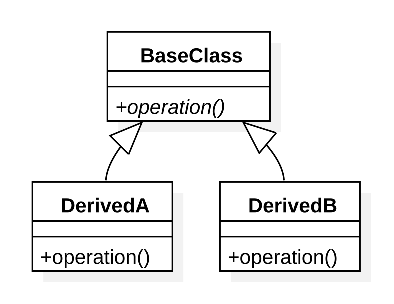
\includegraphics[width=0.35\linewidth]{images/illustrative/runtime polymorphism.eps}
    \caption{Пример реализации динамического полиморфизма виртуального метода на диаграмме классов}
    \label{fig:cpp-runtime-polymorphism-example}
\end{figure}

Важно заметить, что в C++ не включены специальные лексические средства для
описания интерфейсов, как это сделано в таких языках как Java
или C\#. В C++ интерфейс, как элемент неявно включён в виртуальный
класс. В то же время, в тех случаях, когда по каким-то причинам,
интерфейс всё же должен быть обозначен в коде программ сам по себе,
прибегают к идиоматическому представлению посредством объявления абстрактного класса
(или структуры) не содержащего атрибуты, с одними чисто-абстрактными
методами. В этом случае, структура типов выглядит подобно примеру
изображённому на рисунке~\ref{fig:cpp-runtime-polymorphism-example-w-iface},
где интерфейс \texttt{BaseClass} вынесен в отдельный тип
данных~\texttt{BaseClassIFace} обобщающий класс~\texttt{BaseClass},
наследники которого уже и реализуют интерфейс.

\begin{figure}
    \centering
    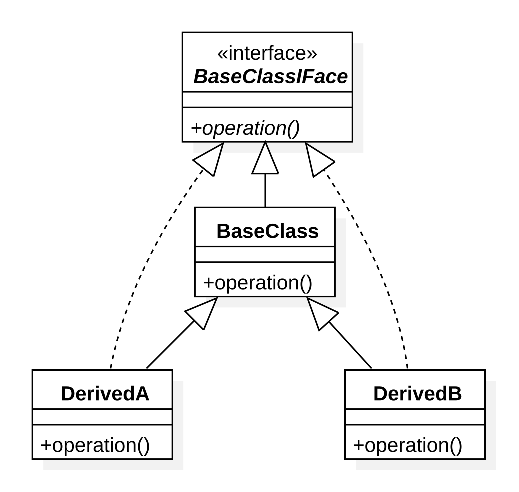
\includegraphics[width=0.5\linewidth]{images/illustrative/runtime polymorphism w iface.eps}
    \caption{Пример реализации динамического полиморфизма в C++ с выделенным интерфейсом на диаграмме классов}
    \label{fig:cpp-runtime-polymorphism-example-w-iface}
\end{figure}

Статический полиморфизм
разрешается на этапе компиляции, обычно через перегрузку функций
и операторов, а также шаблоны \cite{Stroustrup2013}.
Статический полиморфизм в C++ широко используется для достижения
настраиваемого поведения на этапе компиляции без накладных
расходов динамической диспетчеризации. Он реализуется
посредством т.н. traits-типов (в ряде источников -- \emph{свойства},
\emph{шаблоны свойств}), частичной или полной специализации
шаблонов, часто с применением идиомы
\acrshort{sfinae} (англ. \emph{Substitution failure Is not an error},~\cite{Vandevoorde2002-cpp-templates}) -- то есть
механизмом, позволяющим исключать неподходящие
шаблонные инстанцирования при разрешении перегрузок, реализуя,
таким образом систему \emph{классов типов}, подобную той что применяется в
некоторых функциональных языках (Scala, Haskell). Кроме
того, статический полиморфизм может быть достигнут с
помощью идиомы \acrshort{crtp}~(англ. \emph{curiously recurring template pattern},~\cite{Abrahams2005-cpp-metaprogramming}),
при котором классы наследуют шаблон, параметром которого является
сам класс-наследник, что обеспечивает разрешение виртуальной
функциональности на этапе компиляции.

Пример статического полиморфизма с использованием traits-типа
изображён на рисунке \ref{fig:cpp-static-polymorphism-example}.
В качестве полиморфной сущности рассмотрен
класс~\texttt{Subject} параметризуемый типом~\texttt{T}.
Класс~\texttt{Subject} содержит обобщённую программу, в которой
определения типов, вызов конкретных процедур или использование
определённых значений делегируется некоторому шаблонному
типу~\texttt{Traits}, параметризуемому типом~\texttt{T}, в общем
случае не обязательно определённому.
В этом случае, возможно определять полные или частичные (в т.ч.
с использованием \acrshort{sfinae}) специализации типа~\texttt{Traits<T>}
во внешних модулях программ, таким образом дополняя и обогащая
реализации обобщённых алгоритмов в~\texttt{Subject<T>}
соответствующими расширениями. В приведённом примере
инстанцирование шаблона~\texttt{Subject<float>} выводит
конкретную реализацию~\texttt{Subject} на основе информации
предоставленной~\texttt{Traits<float>}.

\begin{figure}
    \centering
    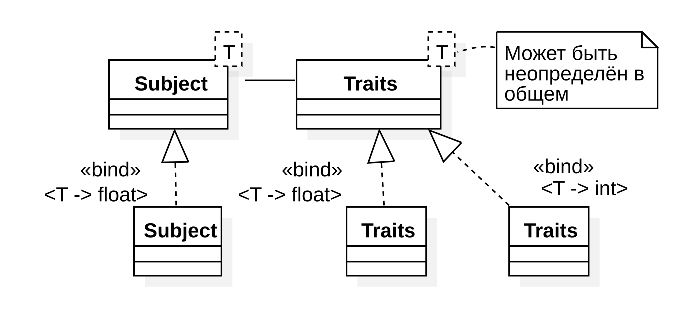
\includegraphics[width=0.7\linewidth]{images/illustrative/static-polymorphism-example.eps}
    \caption{Пример статического полиморфизма на основе шаблона свойств}
    \label{fig:cpp-static-polymorphism-example}
\end{figure}

%Хотя по очевидным причинам, статический полиморфизм эффективен
%с вычислительной точки зрения, с точки зрения практической разработки,
%важно, что реализация статического полиморфизма в C++ посредством
%идиом CRTP и SFINAE представляет собой достаточно сложные для
%сопровождения и отладки лексические конструкции. 
Хотя статический полиморфизм обладает очевидными преимуществами
с вычислительной точки зрения, его практическое использование в C++
сопряжено с определёнными трудностями. Реализация посредством идиом
\acrshort{crtp} и \acrshort{sfinae} приводит к возникновению сложных для сопровождения
и отладки лексических конструкций (грамматика
языка шаблонов исторически вводились в C++ поверх существующего
стандарта языка, и не предусматривает соответствующей
функциональности в виде явных лексических конструкций).
Кроме того, статический полиморфизм характеризуется высокой
инфраструктурной инвазивностью.
По этим причинам,
решение о предоставлении публичным \acrshort{api} точки расширения
реализуемой посредством статического полиморфизма, должно приниматься
в рамках глобальной архитектуры приложений.
%, что делает его использование
%в качестве механизма расширения публичного
%\acrshort{API} оправданным лишь в случае, если такое решение согласовано
%с общей архитектурой системы.


%Основное внимание в последующем изложении уделено описанию обобщённых контекстов и типовых сценариев использования, которые служат основой для разработки
%соответствующих технических решений, с указанием соответствующих
%принципиальных ограничений. Целью главы является выделение конечного
%набора обобщённых решений, охватывающих потребности рассматриваемой
%области в целом и формализующих её типовые задачи, при этом
%предусматривается определение конкретных точек расширения,
%позволяющих адаптировать эти решения к специфическим условиям отдельных
%экспериментов, подсистем и этапов исследований.

\begin{comment}
Дальнейшее изложение сосредоточено на описании обобщённых контекстов и типовых сценариев использования, которые образуют основу для разработки соответствующих технических решений с фиксацией их принципиальных ограничений. Целью главы является выделение конечного набора обобщённых решений (\emph{инвариантов} системы),
охватывающих совокупность потребностей рассматриваемой области и
формализующих её характерные задачи. При этом предусматривается
определение конкретных \emph{точек расширения}, обеспечивающих адаптацию
указанных решений к специфическим условиям отдельных экспериментов,
подсистем и этапов исследований.
\end{comment}
\section{Специфика предметной области}

С момента появления записывающей техники в области высокоэнергетических
экспериментов широкое распространение получила концепция эксперимента с
триггером~\cite{nucl-exp-methods-Grigorev1988}. В её рамках часть
детекторов выделяется в качестве триггерных,
а их сигналы обрабатываются логической функцией для принятия решения о записи
данных на основе откликов быстрых детекторов. Наличие или отсутствие сигналов
от определённого набора детекторов (составляющего лишь часть всего набора
детекторов установки и называемых \emph{триггерными детекторами}),
а также быстрая оценка физических величин
относительно заданных порогов, составляют входные параметры логического
условия. Срабатывание триггера задаёт временную точку отсчёта для
оцифровывания сигналов детекторов в некотором временном окне.
Совокупность данных записанных таким образом упорядочивается в рамках
структуры данных отдельного события. Классическим примером является
эксперимент Коуэна и Рейнеса по регистрации антинейтрино в
1954 году~\cite{cowan1956detection},
в котором основой для выделения событий взаимодействия антинейтрино с
протонами являлось фиксированная временная разница между чувствительными
элементами установки определяемая замедлением нейтронов в веществе
мишени.

Следует отметить, что понимаемый под (оцифрованным) \emph{событием}
набор данных в терминологии информационных систем не всегда строго
соответствует событию в вероятностном смысле. Хотя предполагается,
что события независимы, с определённой частотой — зависящей от
интенсивности исследуемого процесса — возможно наложение статистически
независимых событий во временных интервалах, определяемых длительностью
временного окна и инерционностью откликов детекторов. Этот эффект
естественно обусловлен физическими ограничениями, такими как время развития
электромагнитных и адронных ливней, лавинных процессов, а также
остаточной ионизацией в рабочих объёмах детекторов, сигналами от
вторичных частиц, гало пучка и т.д.

\subsection{Логический триггер}

В экспериментах с большим числом наблюдаемых каналов используется
многоуровневая триггерная система~\cite{nucl-exp-methods-Grigorev1988},
включающая триггеры различных
уровней (например, \emph{L1} — <<\emph{Level 1}>>, \emph{L2} и
последующие). Низкоуровневые аппаратные триггеры реализуются с
использованием аналоговых и дифференциальных схем, а также электроники
с наносекундным и пикосекундным временным разрешением. Их основная
задача --- обеспечить быстрый, предварительный отбор событий по сигналам
детекторов, подавляя таким образом комбинаторный фон сигналов от реакций,
не представляющих физического интереса.

Триггеры более высоких уровней, как правило, реализуются на менее
быстродействующей, но более гибкой цифровой компонетной базе:
на программируемых
логических интегральных схемах (\acrshort{fpga}), а также в виде
программных триггеров, выполняемых на
универсальных процессорах.

%То как именно соотносится программное представление события
%и его программная модель (цифровой образ) --- очень важный вопрос
%архитектуры \acrshort{sw} физического эксперимента.

Особое значение имеет то, каким образом соотносится информация о
событии и его цифровая модель в смысле логического соответствия
статически-типизированным данным. Этот аспект представляет собой ключевой вопрос
архитектуры программного обеспечения физического эксперимента, и его решение
можно можно сформулировать в виде различного рода формальных схем или
диаграмм.

%К примеру, проблема временного перекрытия событий, обусловленного
% чисто статистическими эффектами (для постоянной средней интенсивности
% временные интервалы между событиями подчиняются экспоненциальному распределению).
% В простейшем случае \acrshort{sw} может быть спроектировано таким образом, чтобы после записи событий
% от L1-триггера, события идентифицированные как pile-up отбраковывались и не учитывались в анализе. Такой подход
% не требует разрешать вклады от отдельных статистически-независимых событий. В тех случаях, когда
% интенсивность исследуемой реакции достаточно велика,
% чтобы результат измерений удовлетворял заданному порогу
% статистической значимости, а аппаратура подвержена влиянию
% сложных эффектов приводящих к трудноразрешимым
% неоднозначностям, такой подход оправдан и приводит к
% сравнительно простой архитектуре \acrshort{sw}:
% <<одна сигнатура --- одно событие>>.
% Более сложные случаи подразумевают присутствие в отклике детекторов информации о нескольких событиях, в том числе не обязательно сигнальных. В этом случае программная модель события уже не обязательно соответствует единственному исследуемому событию, хотя для упрощения задач анализа может быть целесообразно сохранить их логическую связь в виде выделенного программного представления.

К примеру, одной из характерных проблем в регистрационных системах является
временное перекрытие событий, обусловленное чисто статистическим
эффектом~(частотной перегрузке, перекрытием
сигналов, англ. \emph{pile-up}): при постоянной средней интенсивности временные
интервалы между событиями подчиняются экспоненциальному
распределению. На практике это означает, что в пределах одного
временного окна могут присутствовать отклики
от нескольких независимых событий.

В простейшем случае программное обеспечение может быть организовано
таким образом, чтобы после записи события, фильтрация, выполняемая при
анализе, отбраковывала записи, идентифицированные как результат
наложения событий, исключая их из дальнейшего анализа.
Такой подход не требует разрешения вклада от индивидуальных
статистически независимых событий и, при определённых условиях, оказывается
вполне обоснованным:
\begin{itemize}
    \item Если интенсивность исследуемого процесса достаточно высока для
    достижения необходимой статистической значимости результатов.
    \item Или если влияние аппаратурных эффектов приводит к возникновению
    неоднозначностей в интерпретации сигналов, которые затруднительно, или
    невозможно устранить алгоритмически.
\end{itemize}

В подобных случаях достигается относительная простота архитектуры \acrshort{sw},
основанной на принципе: <<одна сигнатура — одно событие>>.
В этом случае отношение между оцифрованным сигналом от детектора и
экземпляром события выглядит как простая ассоциация, изображённая на
рисунке~\ref{fig:simple-hit-event}, в котором тип данных~\texttt{Hit}
содержит информацию об отдельных откликах детектора, и его экземпляры
включены посредством композиции в экземпляр события представленный
типом данных~\texttt{Event} выражающим информацию об отдельном событии.

\begin{figure}[ht!]
    \centering
    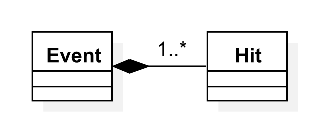
\includegraphics[width=0.25\linewidth]{images/illustrative/simple-event-struct.eps}
    \caption{Простейшая модель отклика детектора в событии}
    \label{fig:simple-hit-event}
\end{figure}

Более сложные сценарии предполагают, что отклик детекторной системы
может содержать информацию от нескольких перекрывающихся событий, включая
как сигнальные, так и обусловленные фоном. В таких условиях программная
модель записанного события инициированного триггерной системой уже не
обязательно соответствует одному акту взаимодействия.
Для упрощения дальнейшего анализа целесообразно
сохранять логическую связность таких данных в виде единого программного
представления (записи) о записи события по триггеру, при этом разделяя вклады
от различных первичных взаимодействий. Вариант реализации приведён на
рисунке~\ref{fig:complex-hit-event}, на котором тип данных события~\texttt{Event}
включает через композицию экземпляры типов данных с информацией об отдельных
откликах, объединяемых посредством агрегации в типе~\texttt{TimeCluster}.
Последний можно представить и в виде класса ассоциации в тех случаях, когда
по каким-то причинам необходима нормализация коллекции~(например, хранение в реляционной~\acrshort{db}).

\begin{figure}[ht!]
    \centering
    %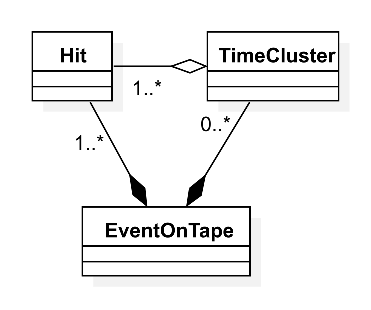
\includegraphics[width=0.33\linewidth]{imgs.view/illustrative/complex-event.eps}
    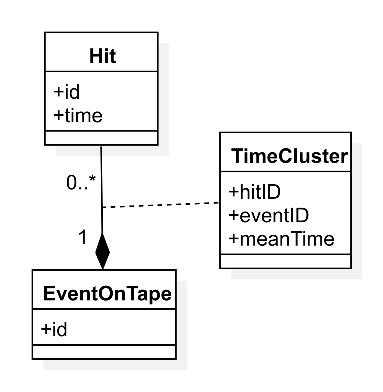
\includegraphics[width=0.33\linewidth]{images/illustrative/hit-assoc.eps}
    \caption{Модель события с разделением откликов во времени с классом ассоциации}
    \label{fig:complex-hit-event}
\end{figure}

В тех случаях, когда разделение откликов во времени неоднозначно, и конкурентные
гипотезы должны рассматриваться одновременно, может потребоваться введение
дополнительных классов ассоциации. На рисунке~\ref{fig:more-complex-hit-event}
вводится дополнительный тип данных~\texttt{Event} агрегирующий информацию о
конкурирующих гипотезах, выраженных посредством различной группировки
временных кластеров.

\begin{figure}[ht!]
    \centering
    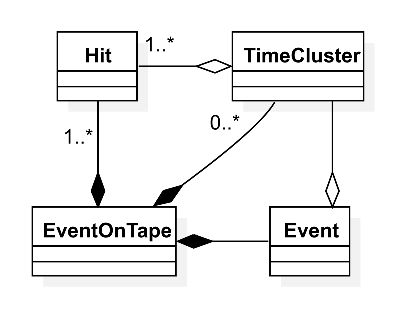
\includegraphics[width=0.33\linewidth]{images/illustrative/more-complex-event.eps}
    \caption{Модель события с разделением откликов во времени представляющая конкурирующие гипотезы}
    \label{fig:more-complex-hit-event}
\end{figure}

Описанные варианты организации модели события и его частей часто встречаются в
иерархии данных при обработке данных физического эксперимента. Другими примерами
могут быть треки частиц, образованные различными комбинациями пространственных
показаний трековых детекторов, амплитуды ячеистых калориметров образующие
пространственные кластеры, сигналы от многослойных трековых детекторов и т.д.
Различные способы представления составных типов данных включают кортежи,
таблицы, реляционных таблицы, структуры и классы, соответствующие выбранным
языковым средам.

\subsection{Модель события}

Среди доступных способов описать модель события в компьютерной программе выделим
следующие, как нашедшие наиболее широкое применение в практике организации
научного \acrshort{sw}:

\begin{itemize}
    \item \emph{Табличная модель}
    %описывает результаты
    %измерения отдельного события в виде кортежа~(строки)
    %%вещественных чисел~$v_i \in \mathbb{R}$
    %в котором
    %информация о принадлежности измерения $v_i$ кодируется
    %индексом~(колонкой)~$i$.
    представляет результаты измерений, относящихся к отдельному физическому событию, в виде
    кортежа (строки), компоненты которого интерпретируются как числовые значения,
    соответствующие различным характеристикам события. Идентификация каждого значения
    $v_i$ осуществляется посредством его позиции или имени соответствующего
    столбца $i$, что позволяет явно связать измеряемую величину с её смысловым
    назначением.
    \item \emph{Реляционная модель}
    %описывает событие в
    %виде наборов строк из взаимосвязанных таблиц между
    %которыми определены реляционные отношения. Для
    %эффективного использования этого подхода необходимо
    %соответствие модели т.н. \emph{нормальным формам},
    %описанным в теории реляционных таблиц.
    описывает событие как совокупность записей, организованных
    в виде взаимосвязанных таблиц, между которыми заданы формальные
    реляционные зависимости. Эффективное применение данного подхода требует
    приведения представления модели к формам,
    обеспечивающим согласованность и непротиворечивость представления,
    что формализуется в рамках т.н. \emph{нормальных форм} реляционной теории.
    \item \emph{Структурная модель} рассматривается в рамках
    т.н. структурного (<<\emph{structured programming}>>, в
    ряде отечественных источников --- \emph{структурированного})
    программирования и вводит иерархическое представление
    поверх реляционной модели посредством специализированных
    выразительных средств целевой среды. Для эффективной
    работы при таком описании не является обязательным
    нормализация отношений модели.
    \item \emph{Объектная модель} исторически рассматривается как
    расширение структурной модели в рамках парадигмы объектно-ориентированного
    программирования (\acrshort{oop}), которая дополняется средствами инкапсуляции,
    наследования и полиморфизма, позволяя задать как структуру,
    так и поведение элементов данных. В рамках этой модели
    физические объекты или события представляются экземплярами
    классов с внутренним состоянием и набором методов взаимодействия.
\end{itemize}

%Заметим, что хотя перечисленные способы не являются
%взаимоисключающими и во многих случаях допускают
%автоматизированную конверсию из одного представления в
%друге (при обязательной рефлексивности данных).
Следует отметить, что указанные модели представления данных не являются
взаимоисключающими и, при условии наличия полной рефлексивной информации
о структуре и семантике данных, допускают автоматизированное преобразование
одной формы в другую.

%Табличный способ и описание посредством реляционной модели
%крайне эффективны при проведении анализа на
%высоком уровне, поскольку современные программные средства
%(такие как \emph{R}, \emph{pandas} (Python), \emph{Matlab} или  % TODO: ссылка
%различные \acrshort{dbms}) предоставляют широкий набор различных агрегатных функций
%для выполнения наиболее частых операций анализа: подсчёта
%моментов распределений над выборками, свёртки, объединения
%таблиц и т.д. Парадигмально, программы на функциональных
%языках оперирующих с табличными данными и списками (\emph{R},
%\emph{Lisp}, \emph{Haskell}) выразительны, лаконичны,
%часто превосходят императивные языки по быстродействию
%за счёт оптимизации на чистых функциях.
%Однако, с точки зрения универсальности
%представления, табличный вид имеет существенный недостаток
%при определении разрежённых~(\emph{sparsed}) данных.
Табличный способ представления данных, а также его формализация
посредством реляционной модели, демонстрируют высокую эффективность
при выполнении физического анализа. Современные высокоуровневые
программные средства анализа данных --- такие
как язык и программное окружение \emph{R},
библиотека \emph{pandas} (Python), язык и программное
окружение \emph{Matlab}, а также различные системы управления
базами данных (\acrshort{dbms}) — предоставляют обширный
набор агрегатных операций, охватывающий типичные задачи: вычисление
статистических моментов по выборкам, выполнение свёрток, объединение
таблиц и прочее.

С парадигмальной точки зрения, программирование на функциональных языках, ориентированных на обработку табличных структур и списков (\emph{R}, \emph{Lisp}, \emph{Haskell}), отличается высокой выразительностью и лаконичностью. В ряде случаев такие языки демонстрируют более высокую производительность по сравнению с императивными подходами, благодаря эффективной оптимизации чистых функций,
оптимизации на хвостовой рекурсии, локализации на стеке.

Тем не менее, в контексте универсальности представления,
табличные структуры обладают существенными ограничениями,
в основном проявляющимися при работе с разрежёнными данными.

%Реляционный вид, хотя и лишён такого недостатка, неудобен при работе
%в императивных языковых средах. Это неудобство
%является определяющим для задач анализа данных физического эксперимента,
%поскольку соответствующая архитектура должна в первую очередь
%отвечать приоритету низкой сложности и динамики прототипов программной
%реализации алгоритмов реконструкции. 
Несмотря на принципиальную возможность учесть разрежённость данных в
рамках реляционного подхода, он малопригоден для практического
использования в императивных языковых средах из-за лексической громоздкости
соответствующих запросов, необходимости всякий раз формулировать условия
объединения. Это обстоятельство является критически важным в контексте
задач анализа данных физического эксперимента, где архитектура
программного обеспечения должна, прежде всего, обеспечивать
низкую сложность и высокую гибкость при прототипировании алгоритмов
реконструкции.
%Функциональное программирование
%и связанное с ним семейство выразительных средств недоступно
%широкому кругу технических специалистов работающих в
%экспериментальной физике и \acrshort{hep}. Так, например,
%специализированный язык для статистических расчётов \emph{R},
%не взирая на популярность в индустрии и у специалистов профессионально занятых статистикой,
%нашёл лишь умеренную популярность среди аналитиков в \acrshort{hep}.

%Основная функция реляционных \acrshort{dbms} --- быстрый поиск, вставка и
%удаление записей в таблицах, оптимизированные для случайного
%доступа. Программная архитектура таких приложений
%выстраивается под работу с индивидуальными записями.
Основное назначение реляционных систем управления базами данных
(\acrshort{dbms}) заключается в обеспечении высокоэффективного поиска, вставки
и удаления записей в таблицах, оптимизированных под случайный доступ
к данным. Соответственно, программная архитектура подобных приложений
ориентирована на работу с отдельными записями.
Напротив, в рассматриваемых сценариях использования чаще всего требуется потоковое
применение алгоритма над большой последовательностью записей.
Для такой задачи оптимизация должна производиться под
последовательную вычитку. Вставка записей в таблицу
на этапе реконструкции производится последовательно, а удаление
записей бывает нужно лишь в отдельных случаях.

Значительно более существенную проблему представляет сложная
иерархия данных физического события: группирование по типам
данных, двунаправленные ассоциации, отношения <<многие ко многим>>
и необходимость частых переходов между уровнями этой иерархии
приводят к большому количеству операций соединения (с точки зрения
реляционной алгебры), созданию промежуточных таблиц и существенно
затрудняют разработку алгоритмов.

Таким образом, применение реляционных таблиц в качестве основного средства
хранения и доступа к данным физического эксперимента не отвечает
основным вариантам использования модели события. Однако, следует
заметить, что в рамках предмета автоматизации физического эксперимента в
целом, существует большое количество сценариев которым
реляционные \acrshort{dbms} отвечают вполне: сопровождение калибровочных данных,
хранение метаданных, журналирование и телеметрия оборудования,
синхронизация пакетных вычислений и т.д.

Напротив, структурная модель вполне отвечает приоритету
простоты и доступности. В рамках такого
описания производят логическое разделение данных события на
семантические группы соответствующие понятиям <<событие>>,
<<кластер>>, <<трек>> и т.д. В рамках структурного
программирования этим понятиям ставят в соответствие
типы данных (посредством специализированных выразительных
средств --- объявляя типы составные данных, таблицы, кортежи).
Такая декомпозиция данных события
отвечает естественным категориям описания алгоритмов, и позволяет
производить разработку прототипов \acrshort{sw} прикладным специалистам.
%за счёт развитого набора сопутствующих выразительных средств
%для выборки и адресации.

Расширением структурного программирования является \acrshort{oop}, вводящее
дополнительные выразительные средства для описания динамического
поведения типов данных. Это расширяет понятие структуры данных
посредством классов, предоставляя таким образом
возможность описывать программу в виде совокупности взаимодействующих
структур данных с инкапсулированным состоянием и полиморфным
поведением.

%Следует подчеркнуть, что в рамках объектно-ориентированного подхода,
%для описания модели события, реализация поведения может относиться
%как к инфраструктуре приложений, так и к их предметному кругу. Например,
%при рассмотрении координатной метке в трековом детекторе, афинные
%преобразования координат могут быть реализованы в объектной модели
%события, что приводит к необходимости описывать согласование связанных
%состояний внутри класса координатной метки (наборы локальных и глобальных
%координат). Информационная избыточность порождённая таким образом,
%будет нуждаться в дополнительных уровнях абстракции, инкапсуляции,
%перенаправления и контроля, что оказывает существенное влияние на
%последующую архитектуру приложений для обработки. Другими подобными
%примерами могут быть любые преобразования индуцированные внешней логикой:
%применение калибровок, нормировки, фурье-преобразования и т.д.
%
%Таким образом, второй важный выбор, который необходимо сделать
%относительно объектной модели: допускается ли избыточность данных в
%модели?

Следует отметить, что в контексте объектно-ориентированного моделирования,
реализация поведения в методах классов, описывающих структуру события,
может быть отнесена к разным уровням ответственности:

\begin{itemize}
    \item \emph{Инфраструктурные аспекты реализации}, предполагающие
    осознанное ослабление изоляции классов с целью упрощения их интеграции
    в алгоритмы. К этой категории относится управление динамической памятью
    и журналирование (в простейшем случае --- стандартные потоки вывода).
    \item \emph{Алгоритмы вспомогательного характера}, выполняемые
    в рамках чётко ограниченных и изолируемых операций, таких как кодирование
    и хеширование ключей коллекций, вставка и удаление элементов.
    \item \emph{Предметно-ориентированные вычисления}, непосредственно
    связанные с логикой физического анализа, включая, например, расчёт
    производных величин (координатные преобразования, вычисление средних значений,
    вероятностные оценки по критерию Пирсона и др.).
\end{itemize}

Так, в частности, рассмотрим класс, представленный на рисунке~\ref{fig:complex-class},
описывающий координатную отметку в плоском
двухкоординатном трековом детекторе. Афинные преобразования координат
вида~$\vec{r} = f(u, v)$ могут быть инкапсулированы в объектную модель события,
как это показано на диаграмме. В этом случае между экземплярами трёх типов
данных --- двумерным и трёхмерным векторами \texttt{Vector2}, \texttt{Vector3},
а также матрицей афинных преобразований \texttt{Transform} --- устанавливается жёсткая
функциональная зависимость, которая должна быть должным образом учтена
внутри класса. Как правило, это реализуется посредством выделения
применения преобразования в приватный или защищённый метод, которые должен быть
вызван с соответствующими аргументами при выставлении локальных координат
(методом \texttt{set\_local\_r()}) или трансформации (методом \texttt{set\_transform()}).

\begin{figure}[ht!]
    \centering
    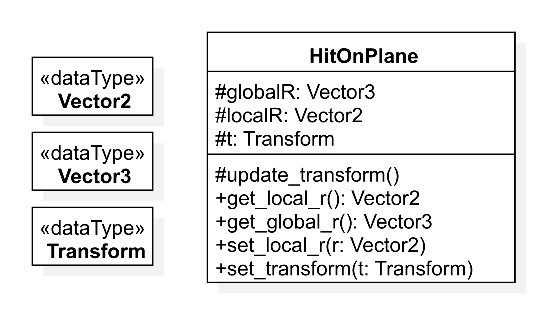
\includegraphics[width=0.45\linewidth]{images/illustrative/complex-hit-class.eps}
    \caption{Класс срабатывания координатного детектора инкапсулирующий координатное преобразование}
    \label{fig:complex-class}
\end{figure}

%В некоторых случаях предметно-ориентированные вычисления сложны, и прибегают к ленивым
%вычислениям, вводя дополнительные флаги контроля, данные кеша и транзитивные хранилища
%для того чтобы снизить потерю производительности на невостребованных элементах состояния.
В ряде случаев предметно-ориентированные вычисления обладают значительной
сложностью и сопровождаются высокой вычислительной нагрузкой. Для повышения
эффективности системы в подобных ситуациях прибегают к ленивым вычислениям,
дополнительно вводя флаги управления, кэш-память и транзитивные хранилища.
Такие меры позволяют минимизировать издержки, связанные с обработкой
невостребованных или редко используемых фрагментов состояния.

%То есть, предметно-ориентированные вычисления требуют реализации механизма согласования
%взаимосвязанных состояний внутри класса координатной метки --- таких, как локальные и
%глобальные координаты в приведённом примере. Возникающая при этом информационная избыточность
%требует введения дополнительных уровней абстракции, инкапсуляции, механизмов
%перенаправления и контроля на уровне события, что оказывает значительное влияние на
%архитектуру последующих программных компонентов обработки. К примеру, при сериализации
%(представление в виде байтовой последовательности для сохранения на диске или ленте)
%и десереализации (восстановлении) описанного в примере объекта принципиально возможно
%появление в программе экземпляра с рассогласованными локальными или глобальными координатами.
Таким образом, предметно-ориентированные вычисления требуют реализации
механизмов согласования взаимозависимых компонентов внутреннего состояния
объекта, как, например, в случае локальных и глобальных координат координатной
метки в трековом детекторе. Возникающая при этом информационная избыточность
предполагает введение дополнительных уровней абстракции и инкапсуляции,
а также реализацию механизмов перенаправления и контроля на уровне
объектной модели события. Эти архитектурные особенности напрямую влияют
на архитектуру и реализацию последующих компонентов программной обработки.

В частности, при \glsprepositional{serialization} (то есть представлении объекта в виде
последовательности байтов для долговременного хранения на внешних носителях)
и последующей \glsprepositional{deserialization} возможно восстановление экземпляра объекта
в рассогласованном состоянии, например, при несовпадении локальных и
глобальных координат вследствие пропуска шагов вычисления или инициализации.

%К аналогичным операциям относятся и другие преобразования на предметно-специфичном уровне
%ответственности, вызванные внешней логикой обработки, включая применение калибровок,
%масштабных преобразований, Фурье-преобразований и т.п.
Аналогичная проблематика возникает и при выполнении других
предметно-специфичных преобразований, инициированных внешними процедурами
обработки, включая применение калибровок, масштабных преобразований,
а также, например, преобразования Фурье и прочие формы предобработки и
согласования представлений.

%Таким образом, (вторым) принципиальным решением при проектировании объектной модели является вопрос,
%насколько \emph{допустима избыточность данных внутри самой модели и как должно быть
%реализовано согласование зависимых элементов}.
В этой связи, одним из принципиальных вопросов при проектировании объектной
модели является определение \emph{допустимого уровня избыточности данных}
внутри структуры события и согласованной с ним \emph{стратегии
согласования зависимых элементов состояния}. Примером наименее избыточных
структур данных могут быть старшие нормальные формы реляционной модели.

%Следует заметить, что архитектура претендующая на высокий уровень общности, не зависящий от конкретного
%эксперимента, не может включать в модель события предметно-ориентированные вычисления ввиду
%многочисленности и противоречивости сценариев использования, а вместо этого должна предоставить
%инфраструктуру в которой определение таких элементов поведения реализуется наиболее упрощено.
Следует подчеркнуть, что архитектура, претендующая на высокий уровень
универсальности и независимости от предметной специфики эксперимента, не может
включать в поведенческое ядро модели события реализацию предметно-ориентированных
вычислений ввиду многочисленности и противоречивости сценариев использования.
Вместо этого она должна предоставлять инфраструктуру, обеспечивающую
максимально простое и декларативное задание соответствующего поведения
в рамках внешней логики прикладного уровня.

Реализацию такого подхода целесообразно осуществить при помощи техник
\glsgenitive{metaprogramming}, опирающихся на интроспективную информацию
о модели события для генерации интерфейсов \acrshort{api}, которые затем
реализуются пользовательскими алгоритмами предметно-ориентированных
вычислений.

Такой подход органично согласуется с предложенной ранее гибридной
методологией разработки ПО, отвечая второму и третьему этапам, в рамках
которых для взаимодействующих алгоритмов фиксируются структурные и
поведенческие аспекты системы.

%В заключении раздела следует заметить, что приведённые рассуждения
%в ограниченной мере справедливы и для т.н. безтриггерных экспериментов.
%В таких экспериментальных установках данные, как правило, обладают той
%или иной степенью гранулярности, обусловленной обычно техническими
%ограничениями. Часто, роль <<события на триггере>> играют временные
%окна (кадры) от потоковых источников данных, которые тем или иным образом
%соотносятся на различных уровнях предобработки (включая циклическую
%буферизацию, различные техники отбора, отыскания корелляций и т.д.),
%прежде чем попасть в персистентные хранилища. Помимо того, что в таких
%системах алгоритмическая насыщенность построения модели события может
%потребовать большей осторожности, чем процедуры реконструкция события,
%попытка построить обобщённую архитектуру предусматривающую работу с данными
%безтриггерного эксперимента обязательно потребует включение в рассмотрение
%систем отбора реализованных на вычислительных платформах различных уровней,
%что существенно увеличит набор вариантов использования системы и её сложность.
В завершение раздела следует отметить, что изложенные выше рассуждения в
определённой степени применимы и к так называемым бестриггерным
экспериментам. В подобных установках исходные данные, как правило,
обладают определённой степенью гранулярности, обусловленной
техническими ограничениями детекторов и средств сбора
информации. Нередко роль событий, зафиксированных триггером
выполняют временные окна (кадры), формируемые потоковыми источниками
данных и соотносимые между собой на различных этапах предварительной
обработки. Эти этапы могут включать циклическую буферизацию,
процедуры быстрого отбора (например, вейвлет-преобразования, поиск по
КД-деревьям), алгоритмы выявления корреляций и другие методы
обработки, предшествующие записи данных в персистентные хранилища.

В контексте данной работы важно, что в таких системах построение
модели события часто сопряжено с более высокой алгоритмической сложностью,
чем в традиционных процедурах реконструкции. Разработка универсальной
архитектуры, способной обрабатывать данные бестриггерных
экспериментов, требует учёта особенностей систем отбора
данных, реализуемых на различных уровнях вычислительной инфраструктуры.
%Это, в свою очередь, существенно расширяет пространство вариантов
%использования программного комплекса и повышает общую сложность
%проектируемой системы.

\section{Сценарии использования}

Выделение сценарных контекстов использования является общим для методологий
разработки \acrshort{fdd} и \acrshort{ddd} и не зависит от конкретного
эксперимента, в то время
как набор конкретных сценариев использования может различаться от
эксперимента к эксперименту.

В этом разделе кратко описаны основные варианты использования программного
обеспечения в экспериментах \acrshort{hep}. Систематизация сценариев
производится в соответствии со следующей (индуктивной) логикой:
\begin{enumerate}
    \item На основе специфики данных выделяются основные ограничения,
    общие для работы с данными в целом, справедливые для всех
    рассматриваемых контекстов использования.
    \item На основе основных этапов жизненного цикла экспериментальных
    данных, выделяются контексты использования.
    \item В рамках перечисленных и ограниченных контекстов, выделяются
    отдельные сценарии использования.
\end{enumerate}

Сценарий использования может представлять собой отдельный модуль,
конкретную численную процедуру, функцию или класс. С точки зрения
обобщённого программирования, важно установить сходства и различия
между одним и тем же сценарием в рамках различных контекстов
использования с тем, чтобы предусмотреть набор точек расширения.

\subsection{Ограничения сценарных контекстов}

В рамках предметной области справедлива следующая специфика данных:

\begin{itemize}
    \item Для анализа редких событий и снижения неопределённости результатов,
    анализ производится на статистике достаточно большого объёма (от
    десятков и сотен терабайт), что не позволяет или существенно затрудняет
    индексирование данных в оперативной памяти вычислительных узлов и
    предъявляет высокие требования к быстродействию программ.
    \item Отдельные (с точки зрения триггерной логики) события в массиве
    данных традиционно рассматриваются как независимые. Это
    позволяет производить операции над отдельными событиями размещёнными в
    оперативной памяти целиком.
    \item Получение выборочной совокупности в анализе опирается зачастую на
    достаточно сложные критерии, включающие расчёты численными методами и
    различные агрегатные алгоритмы, которые затруднительно формулировать
    на языках запросов к реляционным таблицам.
    \item Сценарии обработки как правило формулируются в виде императивных
    программ с большим количеством циклов, ветвлений, внешних коэффициентов,
    запросов из третьих источников. Транзакционный цикл характерный для
    реляционных \acrshort{dbms} избыточен для рядовых сценариев
    обработки или анализа.
\end{itemize}

%В результате, в \acrshort{hep} к настоящему времени реляционные таблицы как основной
%носитель данных не применяется, или применяется крайне ограниченно.
Основным способом представления данных являются упрощённые структуры
типа \texttt{NTuple} или \texttt{TTree}~\cite{ROOT-framework}, представляющие
собой строковые таблицы, со сжатием, буферизацией и оптимизацией для
последовательного доступа (\emph{scan}, последовательный перебор) как основного
способа доступа к данным. Такая модель обусловлена
как структурой данных -- иерархически организованных, но при этом слабо
нормализованных, так и необходимостью применения сложных алгоритмов для
отбора записей в таблицах (событий, информации об отдельных срабатываниях,
физических кластеров, треков частиц). Модель сканирования предоставляет
линейную, предсказуемую модель доступа, легко поддающуюся параллелизации,
в общем не требует встраивания дополнительных индексов,
обеспечивает хорошую переносимость между различными платформами. Кроме того,
для реализации произвольного доступа, модель последовательной вычитки можно
дополнить внешними метаданными, не затрагивая физическое размещение
основных данных в тех случаях, когда формат сам по себе допускает произвольны
доступ.

С этой точки зрения, архитектурное решение относительно основной модели
доступа к данным на раннем этапе заключается в выборе между строковым и
колончатым представлением таблиц, поскольку именно связанные с физической
моделью данных архитектурные  ограничения наиболее трудно преодолеть
впоследствии.

Требования к быстродействию программ актуальны при работе с большими
объёмами данных, типичными для \acrshort{hep}. В то же время, язык используемый для разработки программ должен обеспечивать достаточно широкий набор выразительных
средств, не требующий высокой квалификации для разработки и сопровождения.
Достаточно хорошо этому требованию отвечает семейство языков C. Сопутствующий
набор библиотек предоставляет надёжные реализации численных методов и
широкий набор общих алгоритмов для составления выразительных программ в
императивной логике.

С учётом изложенных особенностей, сформулируем основные черты и ограничения
проектируемого программного комплекса:
\begin{itemize}
    \item Обработка отдельных событий производится в оперативной памяти,
    при этом хранение всего объёма данных возможно в том числе и на
    распределённых хранилищах большого объёма.
    \item Последовательный доступ к потоковым данным из принципиально
    неограниченного источника (потока) используется как основная модель
    доступа к данным. При этом запись соответствующая событию декодируется
    целиком (последовательный доступ для строковых данных как основная
    модель доступа к данным).
    \item C и C++ используются в качестве основных языков реализации
    программ реконструкции.
\end{itemize}

В рамках предложенной методологии разработки, для стратификации вариантов
использования программного окружения для реконструкции событий, необходимо
произвести выделение общих сценарных контекстов. Для этого, рассмотрим
основные этапы жизненного цикла эксперимента с точки зрения применения
прикладного \acrshort{sw}:
\begin{itemize}
    \item \emph{Предварительное численное моделирование эксперимента}. В
    современном физическом эксперименте, моделирование применяется
    при выборе постановки эксперимента для измерения конкретных
    каналов реакций, на этапе разработки технического предложения.
    Оценивается принципиальная возможность проведения измерений с учётом
    выхода реакции, светимости отдельных каналов, геометрии и разрешения
    детекторов. Данный этап в ограниченной форме подразумевает
    реконструкцию событий или применение отдельных алгоритмов.
    \item \emph{Тестирование отдельных детекторов и детекторных сборок}
    (англ. <<research and development>>, R\&D). В рамках этого этапа
    производится тестирование и отладка отдельных конструктивных
    компонент установки: модулей калориметров, трекера. Ограниченно
    применяются (и тестируются) алгоритмы, которые впоследствии будут
    включены в общую реконструкцию событий.
    \item \emph{Набор данных}. Сеансы набора данных обычно упорядочены
    в определённых хронологических интервалах, подразумевающих
    определённое постоянство условий измерения. С этой целью
    необходимо применение развитых средств наблюдения за установкой,
    оперативной диагностики её подсистем.
    \item \emph{Калибровка детекторов}. Может производиться как
    на основе выделенных сеансов набора данных, так и во время
    набора физических данных. Часто включает информацию полученную
    во время R\&D-фазы. Обычно подразумевает реконструкцию и анализ
    в ограниченной форме.
    \item \emph{Анализ физических событий}. На данном этапе необходимо
    наиболее полное знание об условиях измерения, доступ ко всей
    накопленной статистике с целью наиболее полной и достоверной
    реконструкции отдельных физических величин и физических событий
    в целом. Выполняется с привлечением высокопроизводительных
    средств, в окружениях пакетного счёта (\acrshort{htc}, \acrshort{hpc}).
    Результатом измерений являются конкретные значения физических величин,
    функции плотности вероятности, их интегральные оценки,
    доверительные интервалы, результаты проверки статистических гипотез.
\end{itemize}

Важно, что моделирование эксперимента, вообще говоря, должно в конечном
итоге воспроизводить реальные данные, и методически не должно обладать
значимым количеством специфических особенностей и свойств, отличающих
задачи обработки результатов моделирования от задач анализа данных.

На основе этапов жизненного цикла, рассмотрим основные сценарные контексты
в модели потоковой обработки.

\subsection{Анализ физических величин и событий}

Реконструкция физических величин производится на основе откликов детекторов
с использованием предварительно полученных калибровочных
данных, а также различной информации, отражающей известные
характеристики экспериментальных условий, справочной информации и
распределений известных из первых принципов.

Программные интерфейсы соответствующих вычислительных сред, как
правило, оптимизируются с расчётом на данный сценарный контекст, как
наиболее приоритетный, поскольку именно он характеризуется наибольшей
алгоритмической сложностью в рамках всей проблематики анализа данных
физического эксперимента.

В типичном случае сценарий реконструкции предполагает задание
алгоритма, осуществляющего преобразование входных данных, частично
или полностью содержащих информацию о событии и представленную в
терминах объектной модели, в выходной набор данных в том же формате.
Рассмотрим ряд наиболее характерных задач реконструкции событий:

\begin{itemize}
    %\item Выделение зарядовых кластеров на основе набора
    %откликов многопроволочных или микропаттерных газоразрядных
    %детекторов. Принципиально, может быть произведено на основании
    %одной лишь информации из модели события, без использования калибровочных данных.
    \item Выделение зарядовых кластеров на основе откликов многопроволочных или микропаттерных газоразрядных детекторов. Такая операция может выполняться исключительно по информации, содержащейся в модели события, без привлечения калибровочных данных.
    
    %\item Формирование набора зарядовых кластеров,
    %составляющих гипотезу о треке частицы. Для корректного выполнения
    %такой задачи, как правило, необходимо привлечение информации
    %о геометрии детекторов (внешней по отношению к содержащейся в
    %модели события), позволяющей исключить с физической точки
    %зрения маловероятные или невозможные конфигурации.
    \item Формирование совокупности кластеров, составляющих гипотезу о треке частицы. Для этого обычно требуется знание геометрии установки, позволяющее исключать физически маловероятные или невозможные конфигурации.
    
    %\item Аппроксимация выбранной совокупности кластеров моделью трека.
    %В зависимости от используемого метода подгонки (фитирования) может
    %потребоваться учёт дополнительной информации: матриц
    %ковариации, зависящих от пространственного разрешения детекторов;
    %пространственной карты распределения материала внутри детектора,
    %влияющей на эффект множественного рассеяния; а также пространственной
    %карты напряжённости магнитного поля, необходимой при наличии
    %отклоняющих магнитов в спектрометре. Результатом работы
    %подобного (как правило, вычислительно-сложного) алгоритма
    %является набор параметров, характеризующих реконструированный трек
    %частицы: её заряд, массу, кинематические характеристики и ожидаемые
    %отклонения в материале активного объёма.
    \item Аппроксимация выбранных кластеров моделью трека. Здесь могут учитываться ковариационные матрицы, зависящие от разрешения детекторов, карта распределения материала (влияние множественного рассеяния) и карта магнитного поля. Результатом является набор параметров, характеризующих реконструированный трек: заряд, массу, кинематические характеристики и их ожидаемые отклонения.
    
    %\item Оценка энерговыделения от электромагнитного или адронного ливня
    %в веществе калориметра на основе откликов, регистрируемых
    %зарядово-цифровыми преобразователями. Перевод измеренной амплитуд в
    %энергетические единицы осуществляется с использованием функции
    %отклика, параметры которой определяются в процессе предварительной
    %калибровки.
    \item Оценка энерговыделения от электромагнитного или адронного ливня в калориметре по амплитудным сигналам на входах \acrshort{adc}. Перевод амплитуд в энергетические единицы осуществляется на основе функции отклика, параметры которой определяются калибровкой.
    
    %\item Формирование комбинаторных конфигураций элементов
    %модели события для последующей оценки физических гипотез и отбора
    %наиболее правдоподобных интерпретаций с применением иных
    %алгоритмов.
    \item Формирование комбинаторных конфигураций элементов события для проверки физических гипотез и отбора наиболее правдоподобных интерпретаций.
\end{itemize}

%Такие алгоритмы, как правило, допускают формулировки на различных
%уровнях общности, позволяя декомпозицию сложной многосоставной
%задачи реконструкции физического события на более простые
%логически-изолированные этапы.
Подобные алгоритмы допускают формулировку на разных уровнях общности, что позволяет декомпозировать сложную задачу реконструкции события на более простые логически-изолированные этапы. Важной их особенностью является \emph{детерминированность}: преобразование входных данных алгоритмом должно быть в точности воспроизводимым.
На наиболее общем уровне, иерархию вариантов использования в контексте анализа
данных можно свести к трём наиболее общим сценариям, изображённым на
рисунке~\ref{fig:analysis-main-usecases}: оценке функции
плотности вероятности и связанных величин, составлению выборок данных,
и сохранению выборки событий (перенаправлению потока данных).

\begin{figure}[ht!]
    \centering
    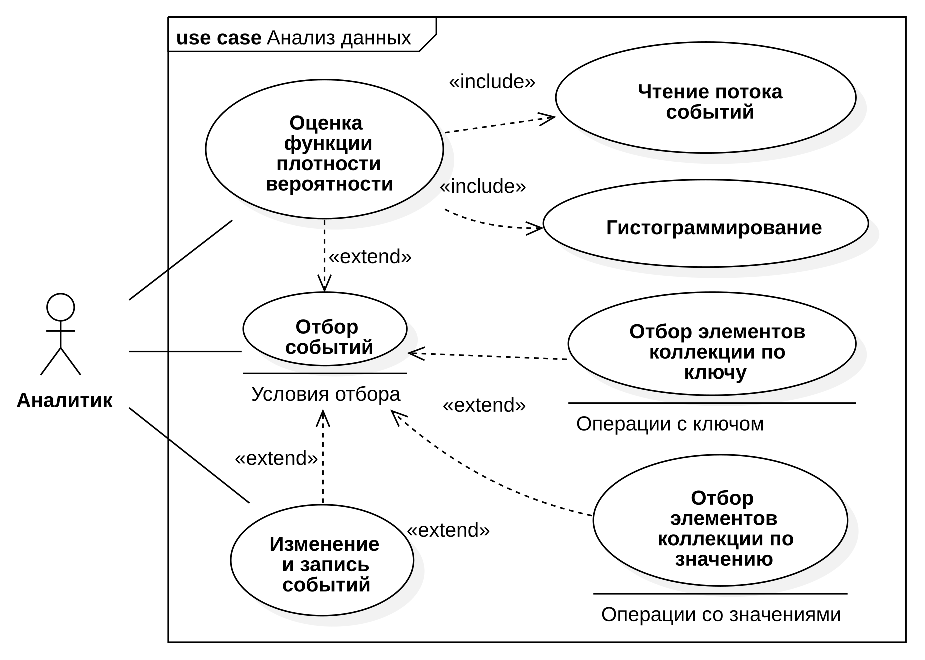
\includegraphics[width=0.85\linewidth]{images/usecases/analysis-usecase.eps}
    \caption{Диаграмма вариантов использования в сценарном контексте анализа данных}
    \label{fig:analysis-main-usecases}
\end{figure}

Для высокоуровневых сценариев отбора событий вводится точка расширения
в которой должен реализовываться отбор, в то время как логика
вычитки и обработки событий может быть реализована в обобщённой
форме. На более низком уровне, во множестве условий отбора, с технической
точки зрения необходимо различать отбор элементов коллекций по
значению и отбор по ключу, поскольку различия в реализации между этими
вариантами весьма существенны.

Главной отличительной особенностью такого контекста является требование к
\emph{детерминированности} вычисления (реконструкции) --
преобразование входных данных алгоритмом должно всегда
оставаться воспроизводимым. Иными словами, преобразование
входных данных должно быть идемпотентно.

\subsection{Сопровождение набора данных}

Другим распространённым сценарием использования программного
окружения является сопровождение эксперимента в ходе набора данных.
В данном случае речь идёт о контроле состояния детекторов и их
диагностике в режиме реального времени (онлайн-реконструкция).
Практически это реализуется посредством случайной выборки небольшой
доли событий из непрерывного потока, что позволяет получать
репрезентативную статистику в ограниченном временном окне, имеющем
фиксированную хронологическую или логическую привязку.

Ключевое отличие данного сценария от полной реконструкции заключается
в приоритете скорости обработки и устойчивости алгоритмов над
точностью и глубиной анализа. Целью становится получение быстрых,
иногда грубых оценок, достаточных для мониторинга работоспособности
установки. В этом контексте алгоритмы реконструкции реализуются в
упрощённой форме, модели заменяются правдоподобным приближением.
Для примера рассмотрим, как задачи из предыдущей группы сценариев
изменяются в рамках данного контекста:

\begin{itemize}
    \item Выделение зарядовых кластеров на выполняется без учёта
    неэффективности чувствительных элементов, рассматривается
    их упрощённая геометрия.
    \item Составление и рассмотрение треков частиц может выполняться
    на основе ограниченного набора вариантов. Например, задача поиска
    трека формулируется без учёта множественного рассеяния, с
    усреднением координат вместо комбинаторного рассмотрения для
    многослойных детекторов
    \item Модель трека аппроксимируется упрощённой функцией
    (с пропагатором прямой или винтовой линией),
    методы Рунге-Кутта не применяются для вычисления ковариации
    в магнитном поле, само поле представлено однородной аппроксимацией
    в конечном объёме
    \item Оценка энерговыделения в откликах калориметров выполняется
    на основе глобальных максимумов сигнала или интегральных сумм ,
    без учёта нелинейностей и нестационарных
    эффектов.
    \item Анализ конкурирующих гипотез может быть заменён случайным
    выбором с целью формирования усреднённой картины.
\end{itemize}

С точки зрения высокоуровневых вариантов использования, данный контекст
представляет собой подмножество контекста анализа данных,
расширенное средствами журналирования и телеметрии, как это изображено
на рисунке~\ref{fig:online-monitoring-usecases-main}.

\begin{figure}[ht!]
    \centering
    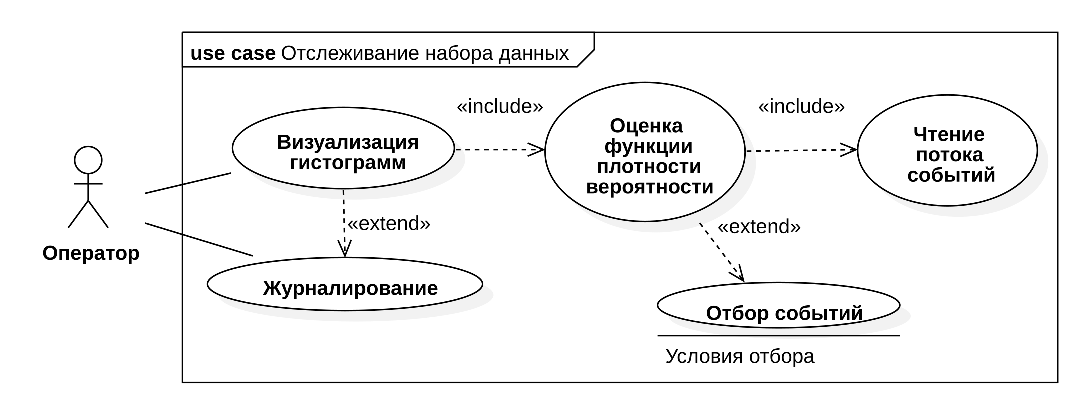
\includegraphics[width=0.95\linewidth]{images/usecases/onlineMonitoring.eps}
    \caption{Диаграмма вариантов использования в сценарном контексте сопровождения набора данных}
    \label{fig:online-monitoring-usecases-main}
\end{figure}

Требования предъявляемые к ПО в данном сценарии отличаются также
и в смысле устойчивости алгоритмов и отказоустойчивости ПО в целом.
Такое ПО предназначено для использования дежурными операторами
экспериментальной установки во время сеансов набора данных. Допустимо
снижение сценарной гибкости и статистической полноты в пользу
производительности и простоты эксплуатации. Требования
детерминированности и идемпотентности преобразований здесь
значительно слабее, чем в предыдущем контексте.

\subsection{Калибровка детекторов}

%В широком смысле калибровка детектора подразумевает отыскание аппроксимации
%\emph{функции отклика детектора}~\cite{exp-methods-Abramov1977}
%в некоторой ограниченной области. Зачастую этот сценарий требует
%получения выборки событий, отвечающей определённому критерию,
%или, напротив, -- максимального ослабления критериев отбора в
%какой-то определённой области. Так, для рассмотренных выше примеров:
В широком смысле калибровка подразумевает восстановление \emph{функции отклика детектора}~\cite{exp-methods-Abramov1977} в ограниченной области. Для этого требуется либо особая выборка событий, либо, напротив, ослабление условий отбора.
В данном контексте рассмотренные ранее примеры выражаются в следующих
сценариях:

\begin{itemize}
    \item Выделение зарядовых кластеров на микропаттерных детекторах
    обычно производится на основе характеристической диаграммы
    отношения амплитуд в области заданной
    некоторым невыпуклым многоугольником. Отыскание этого
    многоугольника представляет собой одну из задач при калибровки
    микропаттерных детекторов, для этой цели различные обрезания
    (временные и координатные) калибруемого детектора должны быть сняты.
    \item После прямых (геодезических) измерений положения детекторов проводят
    т.н. процедуру физического выравнивания (\emph{alignment})
    детекторов установки на основе реконструированной информации о
    треках, уточняя таким образом, геометрию установки, часто с точностью
    намного превышающую прямые измерения. Часто, для этого необходим
    максимально широкий пучок, засвечивающий наибольшую область
    чувствительного объёма детекторов, в широких угловых диапазонах.
    \item Задача реконструкции треков опирается на знание разрешений
    детекторов и карт их эффективности, получение которых представляет
    собой отдельную группу сценариев использования. Для этого реконструкция
    треков производится с исключённым детектором-объектом исследования.
    \item Один из вариантов калибровки калориметров состоит в отыскании
    коэффициентов пропорциональности энерговыделения регистрируемой амплитуде
    на основе известных спектров. Для этого спектры должны быть сначала
    выделены из данных, что составляет отдельную задачу анализа.
    \item Оценивание конкурирующих гипотез для калибровки нередко
    производится с ослабленными требованиями, и в этом смысле часто
    представляет собой даже более вычислительно-ёмкую задачу.
\end{itemize}

В целом, задачи калибровки детекторов во многом пересекаются с задачами
анализа, зачастую, с точки зрения сценариев использования, составляя
их подмножество, как это изображено на рисунке~\ref{fig:usecases-get-calibrations}.

\begin{figure}[ht!]
    \centering
    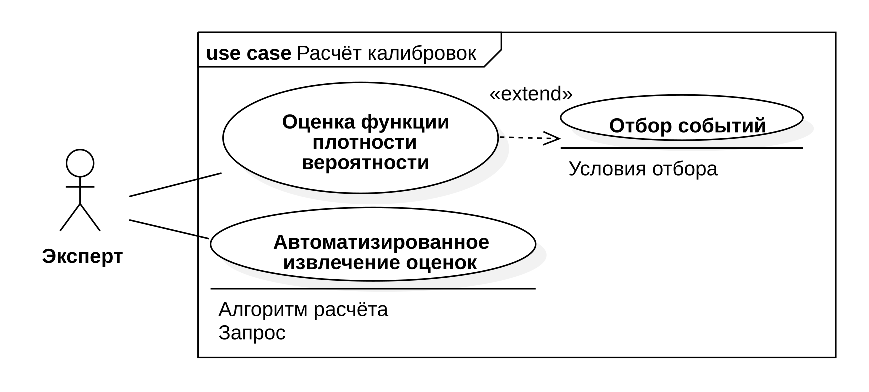
\includegraphics[width=0.75\linewidth]{images/usecases/calibration-usecase.eps}
    \caption{Диаграмма вариантов использования в сценарном контексте извлечения калибровочной информации}
    \label{fig:usecases-get-calibrations}
\end{figure}

Помимо необходимости низкоуровневого доступа к данным объектной
модели (на уровне откликов индивидуальных чувствительных элементов,
формулируемых в точке расширения <<\emph{запрос}>>),
важное прикладное значение могут иметь средства автоматизированного
извлечения информации полученной на основе функции плотности
вероятности, различных спектров и их производных значений, что
целесообразно выделить в отдельный вариант использования с соответствующей
точкой расширения (<<\emph{алгоритм расчёта}>>).

\subsection{Точки расширения на основе вариантов использования}

С точки зрения прикладного программирования, во всех перечисленных
контекстах, варианты использования имеют общие функциональные
элементы, для которых целесообразно предусмотреть обобщённые
реализации воплощающие выбранные черты архитектуры, и
предусмотреть  зависящие от конкретного эксперимента точки
расширения в которых производится реализация конкретной задачи.

\begin{itemize}
    \item  \emph{Идентификация отдельных детекторов} на различных
    логических уровнях -- от элементарных чувствительных элементов
    установки, например, ячейки калориметра, проволоки в зарядовой камере,
    стрипа в микропаттерном детекторе, до детекторных сборок, например
    модульного калориметра как целое, участка трекера вне магнитного
    поля, баррельной части установки для радиальной коллайдерной
    постановки.
    \item Работа с \emph{коллекциями} случайных величин относящихся к
    детекторам или сборкам -- итерирование, формирование выборок,
    различные свёрточные операции и агрегатные функции.
    \item Применение логических условий на случайные величины --
    логическая \emph{дискриминация} случайных величин по определённому
    признаку, выполняемая с использованием идентификаторов детекторов
    или их сборок.
    \item Функция плотности вероятности (или её аппроксимации) --
    для представления различных спектров, статистических
    перенормировок, оценки средних значений и их доверительных
    интервалов. Основным программным инструментом здесь является.
    \emph{гистограмма} (в первую очередь в смысле структуры данных,
    а не графического средства).
\end{itemize}

При этом, конкретные численные процедуры -- вроде численной аппроксимации,
решения СЛАУ, итеративной минимизации функционалов встраиваются в такую
парадигму как отдельные элементы.

Номенклатура детекторов и логическая топология определяются
конкретной установкой, иерархией её узлов и подсистем. Важно, что
объектная модель события во многом подчинена этой иерархии:
оцифрованные сигналы от отдельных чувствительных элементов
объединяются в рамках коллекций в сущности, соответствующие
физическим понятиям (зарядовый кластер, ливень в калориметре,
трек), логически отвечающие отдельным детекторам (станция трекера,
модуль калориметра, трекер). Попытка обобщить эти отношения в рамках
какой-нибудь одной системы скорее всего будет создавать больше сложностей
чем решать.

По этой причине, номенклатура детекторов и объектная модель должны
быть вынесены в точки расширения, в то время как коллекции и операции над
ними, включая логическую дискриминацию, целесообразно объединить в
рамках обобщённых алгоритмов, задающих инварианты системы.

\section{Архитектурные инварианты}

Архитектурный инвариант (англ. \emph{architectural contraint}
\cite{shaw-architecture-1996, bass-architecture}) --
это свойство программной архитектуры, которое должно
сохраняться независимо от изменений в деталях реализации или
развития системы. На основе требований сформулированных ранее,
выделим архитектурные инварианты предлагаемого решения:
\begin{itemize}
    \item Модульность -- отдельные компоненты должны
    быть изолированы так, чтобы можно было заменять
    один алгоритм реконструкции на другой без
    переписывания всей системы.
    \item Детерминированность обработки событий:
    алгоритм реконструкции при одинаковом входе
    всегда даёт одинаковый выход.
    \item Соответствие модели события и триггерной
    логики: структура данных события всегда отражает
    триггерное условие, по которому оно было записано.
    \item Потоковый доступ к данным: вся архитектура
    опирается на последовательную обработку событий.
    \item Независимость предметно-ориентированных
    вычислений от ядра системы -- логика физических
    расчётов (например, калибровки, аппроксимации
    треков) не должна входить в поведенческое ядро
    модели события, а реализуется через внешние алгоритмы
    и плагины.
    \item Иерархическая структура объектной модели
    события.
\end{itemize}

В качестве механизма обеспечивающего инвариантные свойства системы
рассматривают т.н. шаблоны (паттерны) проектирования~(\emph{architecture patterns}, \emph{software design patterns})~\cite{gof1994design-patterns}.
Шаблоны проектирования представляют собой не только типовые
решения, но и формализуют основные архитектурные ограничения
системы: они фиксируют допустимые способы взаимодействия
компонентов, ограничивают допустимые механизмы расширения и тем
самым обеспечивают сохранение инвариантов архитектуры при развитии
программного комплекса. Каждое применение шаблона проектирования можно
рассматривать как задание архитектурного инварианта: он ограничивает
пространство возможных реализаций, но гарантирует сохранение
устойчивых свойств системы — модульности, слабой связности, управляемости
расширений.
%Книга представляет собой первую попытку выделения и систематизации
%структур компьютерных программ в объектно-ориентированной парадигме,
%направленных на решение задач для которых вводится классификация по
%области применения (основные, структурные, порождающие, поведенческие),
%и типовым вариантам использования.

\subsection{Конвейерный шаблон}

Идея декомпозиции сложной процедуры на последовательность
обработчиков, каждый из которых действует независимо, выполняя
элементарную задачу над общей структурой данных, широко применяется
при организации сложных вычислительных систем достаточно давно.
В информатике, возникновение идеи и
связанной с ней терминологии можно отследить до архитектуры ранних
компьютеров (например, БЭСМ-6, \cite{smirnov-besm6}).

Классическим вариантом шаблона является
<<цепочка обязанностей>>~(\emph{chain of responsibility}).
В исполнении <<цепочки обязанностей>> прежде всего направлен на
разделение отправителей и получателей запросов в цепочке обработчиков,
архитектурный шаблон <<конвейер>> (\emph{pipes and filters})~\cite{Buschmann-patterns-vol1}
структурирует последовательную обработку данных посредством компонуемых
этапов. Хотя эти две концепции обобщают линейную последовательность
обработки, их мотивация различается:
в первом случае акцент сделан на делегировании управления потоком с
с явным указанием ответственности,
во втором важнейшим аспектом является преобразование потоковых данных.
Разделение ответственности удобно при формировании сложной и разветвлённой
логики приложений во время выполнения, и наиболее широкое применение шаблон
<<цепочка обязанностей>> нашёл при обработке событий графических
пользовательских интерфейсов, где часто применяется для динамического
связывания реакций компонентов приложения с событиями пользовательского
ввода.

Основная мотивация для использования шаблона <<конвейер>> по~\cite{Buschmann-patterns-vol1}:

\begin{itemize}
    \item Система должна позволять усовершенствования за счёт
    изменения последовательности обработчиков (на высоком уровне)
    \item Допускается повторное использование отдельных обработчиков
    в различных сценариях
    \item Несмежные обработчики не обмениваются информацией (т.е.
    передача элемента данных должна производиться от одного обработчика
    к другому, без пропусков)
    \item В системе предусмотрены различные источники входных данных,
    (файл, сетевое соединение, поток ввода).
    \item В системе должна быть предусмотрена возможность представления
    или хранения результатов различными способами
    \item Явное хранение промежуточных результатов для дальнейшей
    обработки не требуется для высокоуровневых операций
\end{itemize}

Следует также упомянуть полезное свойство <<Конвейера>>, рассматриваемое
в контексте параллельных
алгоритмов~\cite{Mattson2005-parallel-patterns, smirnov-besm6}:
когда индивидуальные обработчики действительно независимы, возможно
запускать их на параллельных системах.
% более толковое изложение (чем в книге на стр.103) у авторов на сайте:
%   https://www.cise.ufl.edu/research/ParallelPatterns/PatternLanguage/AlgorithmStructure/Pipeline.htm
% следует ли здесь подвести мотивацию к обобщённому алгоритму pipe-T?

С точки зрения реализации алгоритмов обработки, конвейерный шаблон
подразумевает реализацию обратной логики управления обработчиками.
Обработчик может инициировать прекращение обработки отдельного сообщения.
Этот результат выполнения обработчика соответствует
дискриминации физического события. Кроме того, обработчик может
инициировать остановку процесса перебора в целом, что соответствует,
например, задаче поиска события в наборе.

\subsection{Коллекции и идентификаторы}

Организация модели подразумевает все возможные типы
ассоциации: одиночное и множественное агрегирование и композицию, а
также отношение наследования между типами данных, и наследование от
коллекций. 

Рассматривая C++ в качестве основной целевой среды для генерации кода,
целесообразно воспользоваться контейнерами стандартной библиотеки
шаблонов для реализации коллекций, представляющими собой обобщённые
реализации коллекций.

Важным следствием выбора C++ в качестве основной среды является
предоставляемый всеми контейнерами стандартной библиотеки набора
выведенных типов, среди которых всегда присутствует идентификатор
играющий роль синтетического ключа (тип значения для последовательностей,
кортеж пары для карт и хэш-таблиц). Тогда индексирование коллекций
можно ограничить случаями с естественным ключом, что улучшает
читаемость прикладных программ и не приносит никаких накладных
расходов.

С алгоритмической точки зрения можно выделить три независимых качества,
которые нужно контролировать при задании типа коллекции по
естественному ключу.
\begin{itemize}
    \item Свойство упорядоченности по значениям естественного ключа
    в коллекции определяет эффективный алгоритм поиска в коллекции.
    \item Разряжённость значений ключа определяет, заполняет ли
    множество значений ключа в коллекции интервал значений без пропусков.
    \item Неоднозначность соответствия.  Во многих практических случаях
    естественный ключ должен ссылаться на множество элементов.
\end{itemize}

Поскольку каждое качество представлено в виде логического флага, определим
на их основе набор меток (англ \emph{tags}) которые впоследствии используются
метапрограммой выводящей тип коллекции на основе спецификации типа данных:
упорядоченность -- \emph{ordered}, разряжённость -- \emph{sparse} (от
англ. \emph{sparsedness}), неоднозначность -- \emph{ambig} (\emph{ambiguity}).

Три логических свойства образуют набор из восьми возможных комбинаций. Каждой
комбинации ставится в соответствие определённый контейнер стандартной
библиотеки шаблонов.

\begin{table}[ht]
    \centering
    \begin{tabular}{r|l}
        Метки & Контейнер STL \\ \hline
        \emph{ordered} & \texttt{vector} или \texttt{map} \\
        \emph{sparse} & \texttt{unordered\_map} \\
        \emph{ambig} & \texttt{unordered\_multimap} \\
        \emph{ordered, sparse} & \texttt{map} \\
        \emph{ordered, ambig}  & \texttt{multimap} \\
        \emph{sparse, ambig} & \texttt{unordered\_multimap} \\
        \emph{ordered, sparse, ambig} & \texttt{multimap}
    \end{tabular}
    \caption{Соответствие типов коллекций}
    \label{tab:placeholder}
\end{table}

Нужно заметить, что требования к типу данных ключа необходимо и достаточно
связаны с операциями которые он поддерживает. Помимо того, что
для любого ключа должна быть определена операция
сравнения ($a \ne b$), упорядоченные коллекции требуют
определения отношения порядка ($a < b$), неупорядоченные --
определения хэш-функции.

Задание коллекций через такую спецификацию меток позволяет
определить и обобщённую реализацию схему реляционных
таблиц.

\subsection{Шаблон подписки}

Калибровочные данные должны быть доступны как в процедурах
реконструкции событий, так и при онлайн-сопровождении
набора данных и при извлечении других калибровочных данных.
При этом источники информации могут быть различными:
результаты отдельных процедур анализа, внешние базы
данных, сетевые сервисы. В рамках выделенных сценариев
использования очевидна необходимость в архитектурном решении,
обеспечивающем доставку актуальных калибровочных данных
среди множества потребителей без жёсткой привязки этих
потребителей к источникам, что задаёт две точки
расширения -- тип калибровочной информации, который
целесообразно учесть через статический полиморфизм,
и поведение компонента при обновлении калибровочной информации.

Такая задача естественным образом решается в рамках архитектурного
шаблона <<издатель/подписчик>> (англ. \emph{publisher/subscriber}).
Его применение опосредует прямые зависимости между
модулями: компоненты, публикующие новые значения калибровок
(издатели), агностичны к конкретным потребителям (подписчиков).

Данное решение отвечает следующим архитектурным инвариантам:
\begin{itemize}
    \item Модульность. Издатели и подписчики инкапсулируют свои роли,
    взаимодействуя только через контракт интерфейса, что облегчает
    замену или расширение отдельных модулей.
    \item Поддержка потоковой модели обработки данных.
    Калибровочная информация распространяется синхронно, при получении
    события с определённым хронологическим идентификатором и
    не нарушает последовательную логику обработки потока
    событий, не нарушая детерминированности самих алгоритмов
    реконструкции.
    \item Гибкость точек расширения. Подписка на калибровочные
    данные может осуществляться произвольными модулями, включая
    вновь разработанные алгоритмы, без изменения ядра системы.
    \item Независимость предметно-ориентированных вычислений от
    ядра. Ядро системы агностично к конкретной логике обработки
    калибровок.
    \item Стандартизированные интерфейсы данных. События публикации
    калибровочных параметров унифицированы.
\end{itemize}

Шаблон отвечает следующим сценариям:
\begin{itemize}
    \item Источник получающий событие с хронологической меткой
    вызывает каскадное обновление всех алгоритмов реконструкции,
    подписанных на определённый тип данных.
    \item В ходе набора данных подписчики имеют актуальные
    калибровки без необходимости ручной синхронизации.
    \item Специализированные процедуры анализа могут использовать
    калибровки, подписываясь на выделенные каналы
    публикации (реализована возможность пользовательского
    переопределения калибровочных данных для подмножества компонент).
\end{itemize}

Необходимо отметить, что в практической реализации критически важно
учитывать, что между информацией различных типов существуют
зависимости. Корректное разрешение зависимостей целесообразно
реализовать на уровне ядра системы. Таким образом, при инициации
рассылки калибровочной информации, компонент <<издатель>> должен
выполнить топологическую сортировку (например, алгоритмом
Кана~\cite{kahn-tsort}).

Таким образом обеспечивается согласованность данных во всех
рассмотренных сценариях использования.

\section{Существующие программные решения}

В данном разделе коротко описаны основные существующие
технические решения, дополняющие понятийный аппарат разрабатываемого
программного окружения в рамках рассматриваемой гибридной методологии.
%С точки зрения прикладного программирования, рассмотренные решения
%формируют основу технологического стека

\subsection{Программы прикладного уровня}

Рассмотренные в данном разделе программные средства
направлены на решение конкретных локальных задач и образуют стек
технологий, обычно в том или ином виде фиксируемый исследовательской группой.
Предлагаемый программный комплекс предполагает использование этих
или подобных средств для решения конкретных задач (таких как, например,
хранение статистики или реконструкция треков).

\subsubsection{ROOT}

ROOT~\cite{ROOT-framework} представляет собой специализированное
объектно-ориентированное программное окружение, разработанное в CERN
для обработки и анализа данных в области экспериментальной физики
высоких энергий. Архитектура ROOT построена вокруг иерархии классов,
рассчитанной на полный цикл работы с данными, включая файловый и
сетевой ввод/вывод, поддержку сериализации сложных объектов
посредством динамического полиморфизма, а также фильтрацию данных
средствами встроенного предметно-ориентированного языка~(TFormula).

Ключевой особенностью является интеграция интерпретатора C++~(CINT и Cling),
позволяющая сочетать динамическое выполнение кода с полным доступом
к \acrshort{api} окружения без необходимости предварительной компиляции
программ. Такая интерактивность, по замыслу авторов, должна обеспечивать
совмещение простоты разработки сценариев и быстродействие
скомплированных программ в едином окружении, развивая идею, предложенную в
рамках языка Smalltalk, — тесную интеграцию языка, среды
выполнения и среды разработки в единую систему посредством
обязательных механизмов интроспекции типов.

Системный дизайн ROOT ориентирован на работу с большими
объёмами и сложной структурой данных, что выражается в
поддержке специализированных форматов хранения, оптимизированных
под последовательное чтение и реализацию поисковых запросов
последовательным перебором, механизмах
эффективного последовательного доступа и выборки, а также в
развитой инфраструктуре статистических и графических инструментов.

При этом необходимо отметить в качестве основной архитектурной
особенности тот факт, что ROOT не предоставляет интерфейсов в классическом
смысле \acrshort{oop}, и с точки зрения типологии \acrshort{sw}
является скорее набором библиотек (а не <<фреймворком>>), то есть
не предполагает наличия сложных алгоритмов с обозначенными точками
расширения.

В рамках данной работы большой практический интерес
представляют отлаженные и хорошо
оптимизированные предметно-ориентированные компоненты ROOT
предоставляющие подсистему хранения и передачи данных, программные
модели различных гистограмм и инструменты для работы с ними,
некоторые численные алгоритмы, такие как универсальный генератор
\texttt{TFoam} или система численной минимизации \texttt{Minuit}.

\subsubsection{Geant4}

Geant4~\cite{allison-recent-g4-2016} представляет собой
объектно-ориентированный программный инструментарий, предназначенный для
моделирования прохождения частиц через вещество и применяемый в
экспериментальной физике частиц, космических исследованиях и
медицинской физике. Архитектура Geant4 основана на системе классов C++,
описывающих физические процессы, типы частиц, геометрию
детекторов, материалы и пользовательские действия.

Geant4 предоставляет обширный набор реализаций вероятностных
генераторов описывающих наибольшее количество известных на
сегодняшний момент процессов в физике частиц.

Его программная архитектура документирована и построена на основе
многостадийного алгоритма трассировки частиц с обозначенными точками
расширения, выраженными посредством интерфейсов в абстрактных
классах C++ -- в схеме классического <<фреймворка>> \acrshort{oop}.
Конфигурирование моделирования осуществляется в этих точках расширения
путём комбинирования предопределённых или пользовательских списков
физических процессов, задания конфигураций детекторов и определения источников первичных частиц, естественно опираясь на полиморфизм и наследование объектного
представления соответствующих классов-реализаций.

В рамках данной работы Geant4 рассматривается как основная среда для
моделирования методами Монте-Карло.

\subsubsection{GenFit2}

Библиотека GenFit2~\cite{Genfit2_Rauch_2015} предоставляет расширяемый
набор инструментов для реконструкции треков заряженных частиц
в экспериментах физики высоких энергий. Проект развивался
в сообществе экспериментов PANDA~\cite{panda-collaboration} и
Belle~II~\cite{belle-ii}. Основу библиотеки составляет реализация
фильтра Калмана~\cite{kalman-1960} и его модификаций,
применимых в условиях неоднородного
магнитного поля (пропагация ковариации методами Рунге-Кутты~\cite{StrandlieJacobians}) и
сложной геометрии детекторов (учёт множественного рассеяния и ионизации).
Поддерживается линейная и нелинейная формы фильтра
Калмана, реализованы различные процедуры итеративного уточнения
трека.

Архитектурно GenFit2 опирается на собственную локальную объектную модель
события,
выделяя статическую и динамическую информацию о треке в раздельные классы
в тесной связи с формализмом фильтра Калмана. Таким образом, входные
данные представляются набором измеренных состояний (в терминах координат,
импульсов и их ковариационных матриц), а результат работы фильтра Калмана
содержится в динамических транзитивных объектах.

GenFit2 использует вокселизацию ROOT для представления трёхмерной карты
распределения вещества,
использует его систему типов для динамического полиморфизма и использует
реализации методов Рунге-Кутты для трассировки ковариационных оценок
через карту магнитного поля.

Таким образом, инфраструктурно, библиотека предоставляет
публичный~\acrshort{api}, позволяя вмешиваться в основной процесс
реконструкции трека. Так, в частности, реализован алгоритм
General Broken Line~\cite{gbp-kleinwort} для реконструкции трека,
не нарушающий основную логику библиотеки.

\subsubsection{Millipede II}

В экспериментах нуждающихся в точной геометрической информации,
геодезические измерения зачастую и по разным причинам, неспособны обеспечить
необходимый уровень точности. В связи с этим особую актуальность имеет
задача геометрического выравнивания детекторов установки,
заключающаяся в уточнении их координат, углов поворота и различных
внутренних параметров (таких, как, например, множители Лагранжа
при провисании анодных проволок в газоразрядных камерах) на основе
реконструированных треков. Существуют несколько различных подходов
к решению этой задачи, за которой закрепилось узкое понимание
термина \emph{выравнивание}~(англ. \emph{alignment}).

Millepede~II\cite{millipede-blobel2009} -- это специализированная
библиотека, предназначенная для выравнивания трековых детекторов.
Она решает задачу одновременного подбора глобальных параметров
(геометрические положения и ориентации элементов детектора,
калибровочные константы) и локальных параметров (параметры
отдельных треков частиц). Основная особенность метода
заключается в том, что задача сводится к решению большой
переобусловленной \acrshort{sle} с блочной матрицей, где блоки, относящиеся
к локальным параметрам исключены аналитически.
Таким образом достигается эффективная редукция размерности
задачи и возможность обращения матриц больших порядков.
Оригинальный численный метод обращения и итеративного
решения разреженных блочных матриц, предложенный
В. Блобелем, является ключевой инновацией Millepede II,
позволившей использовать его как стандартный инструмент
выравнивания во многих экспериментах.

\subsection{Инфраструктурные решения и экосистемы}

Существуют решения, претендующие на сопровождение
полного жизненного цикла физического эксперимента.

\subsubsection{Gaudi}

Gaudi~\cite{gaudi-framework-1} представляет собой модульное
объектно-ориентированное программное окружение, разработанное
в CERN для организации систем обработки данных в экспериментах
физики высоких энергий. Архитектура Gaudi
изначально ориентирована не на полный цикл работы
с данными в рамках одного монолитного окружения, а на
построение приложений из набора взаимодействующих компонентов,
выполняющих функции ограниченные интерфейсом. Таким образом
архитектура выполнена в виде компонентной модели с чётко
определёнными интерфейсами задающими точки расширения.

Gaudi реализует инфраструктуру,
включающую управление жизненным циклом компонентов,
планирование и диспетчеризацию обработки событий, доступ к
условиям и метаданным, а также взаимодействие с системами
ввода-вывода. Прикладная логика оформляется в виде
алгоритмов и сервисов. Этапы конфигурирования и инициализации
приложения разделены.

Системный дизайн Gaudi опирается на модель события с динамической
интроспекцией, поддержку распределённых
вычислений (\acrshort{htc}) и интеграцию с внешними системами хранения,
базами данных.

Проект строится вокруг следующей классификации
источников данных, представленных в виде сервисов:
\begin{itemize}
    \item Сервис сообщений, предоставляющий
    интерфейс~\texttt{IMessageSvc}, реализующий задачи
    журналирования.
    
    \item Сервис данных события~(\texttt{EventDataSvc}),
    реализующий доступ к транзиентному хранилищу данных,
    разделяемом между алгоритмами в рамках обработки одного
    события. Сервис предоставляет унифицированный
    способ получения и размещения элементов объектной модели
    события.

    \item Сервис калибровочных данных, условий и геометрии
    детектора (\texttt{DetectorDataSvc}), предоставляющий
    статическую информацию о структуре детектора, его
    параметрах, а также условия проведения
    измерений.

    \item Сервис преобразования данных (\texttt{ConversionSvc}) и
    механизм сериализации/десериализации, обеспечивающие независимость
    логики реконструкции от конкретного формата хранения данных.

    \item Планировщик (\texttt{IScheduler},
    %или более современный \texttt{Gaudi::Hive::WhiteBoard})
    отвечающий за порядок вызова алгоритмов и управление
    их зависимостями на основе графа исполнения.
    %, что особенно
    %важно в условиях параллельной или многопоточной обработки событий.
\end{itemize}

В рамках данной работы Gaudi рассматривается в основном
в качестве ближайшей функциональной альтернативы.

\subsubsection{FairROOT}

FairRoot и FairSoft~\cite{fairroot-AlTurany-2012} образуют
\emph{экосистему} программного обеспечения, разработанную
в рамках FAIR (Facility for Antiproton and Ion Research,
GSI, Дармштадт, \cite{FAIR-techreport}) для моделирования,
реконструкции и анализа данных в современных экспериментах по
физике высоких энергий и ядерной физике.

Целью данного проекта является гарантия совместимости
инструментов объединённых в рамках общих протоколов и форматов.
Так, например, ROOT и Geant4 имеют не вполне совместимые системы
описания конструктивной полнотелой геометрии и используют
разные алгоритмы вокселизации. С целью решения этой проблемы
авторы проекта вводят дополнительный слой абстракции реализованный
в выделенной библиотеке VNC (Virtual Monte-Carlo) и специализируют
его интерфейсы в расширенном описании в рамках собственных обобщающих
программных моделей.

Поскольку подобная активность всегда связана с поиском компромиссов
между активно меняющимися программами, разрабатываемыми третьими
лицами, подобное начинание требует утверждения версий
проектов включённых в такую экосистему. FairSoft -- это программный
стек, включающий внешний набор библиотек и
инструментов, необходимых для работы FairRoot. В неё входят
ROOT, Geant4, VMC, инструменты сериализации и удалённого вызова
процедур. FairSoft призван обеспечивать стандартизированное
и согласованное окружение.

Создание такой экосистемы продиктовано потребностью
крупных коллабораций %(например, PANDA, CBM, R3B на FAIR,
а также ряде других экспериментов в Европе и за её пределами)
в едином, воспроизводимом и модульном программном окружении,
объединяющем моделирование, реконструкцию и анализ в стабильной
форме.

\section{Спецификации}

Описанные в главе принципы можно свести в перечень
конкретных спецификаций, которым должна отвечать программная
система с требуемыми архитектурными инвариантами.

\subsection{Обработка данных}

Обобщённая реализация конвейерного шаблона проектирования, опирающегося
на модель физического события представляет собой универсальный компонент
для систем обработки данных эксперимента с триггерной
системой.

С учётом изложенных ограничений на модель события,
описание составного типа данных должно включать:
\begin{itemize}
    \item Имя типа -- строковый идентификатор совместимый
    с определением типа в C++ и стандартом именованием таблиц
    в \acrshort{dbms}.
    \item Список атрибутов (полей), состоящий из
    упорядоченного набора кортежей из трёх элементов, включающих
    имя, тип данных и описание атрибута. Имя атрибута
    должно быть совместимо с определением атрибутов структур в C++.
    Тип атрибута должен соответствовать множеству типов для которых в
    программном окружении посредством статического полиморфизма определены
    основные операции конверсии, серелиазции и десериализации.
\end{itemize}
Дополнительно, описание составного типа данных может включать:
\begin{itemize}
    \item Документацию к типу,
    \item Родительский тип,
    \item Список динамических атрибутов типа.
\end{itemize}

На основе такой спецификации, для набора типов,
среди которых указан один корневой тип хранимого события должны
выводиться следующие объявления и реализации:
\begin{enumerate}
    \item Объявление всех типов данных (в C++ -- декларации классов)
    \item Для реализации процедур на основе статического
    полиморфизма -- объявление
    шаблонных свойств объявленных типов (англ. \emph{template traits}) для
    перебора атрибутов, с указанием имени атрибута, типа, порядкового
    номера,
    \item Интерфейс источника данных реализующий генератор
    экземпляров корневого типа (в случае C++ -- базовый класс
    источника данных),
    \item Интерфейс реализующий конвейерный шаблон
    относительно корневого типа и его реализацию (перебор событий
    с обратной связью от обработчиков),
    \item Интерфейсы обработчиков экземпляров типов данных (англ. \emph{handler}),
    в частности интерфейс обработчика данных принимающих экземпляр
    корневого типа (в случае C++ -- базовый класс обработчика
    событий).
\end{enumerate}

Требование №2 связано с тем, что в C++ на уровне семантики шаблонов
(и, вообще, в рамках стандартных средств языка)
отсутствуют средства для перебора набора полей структуры или класса
в виде набора кортежей (имя, тип). Если каким-либо образом предоставить
такую информацию, возникает возможность определять рекурсивные
метафункции, способные обходить всю иерархию типов во время компиляции.
В частности, если для всех типов атрибутов определены
операции сереализации и десериализации, сериализуемость составного
типа реализуется процедурно, на основе шаблонных свойств.

\subsection{Калибровочные данные}

Обобщённая реализация интерфейсов доставки калибровочных данных
должна быть представлена в виде реализации шаблона <<издатель/подписчик>>.
Оба компонента выражаются явно, в виде соответствующих классов.

Добавление нового типа калибровочных осуществляется средствами статического
полиморфизма -- на основе типа данных выводится реализация абстрактного
типа подписчика. Компоненты реализуют поведение подписчика посредством
динамического полиморфизма.

В случае зависимостей между типами данных, вычисление корректного порядка
оповещения подписчиков должно выполняться издателем.

\subsection{Цикл разработки}

Цикл разработки опирающийся на предложенные решение предполагает
инкрементную модель расширения функциональности, как это описано
в методологии \acrshort{fdd}. В рамках сравнительно
коротких циклов
осуществляется прототипирование и реализация требуемой
функциональности. На завершающем этапе компонент (обработчик
конвейера или утилита) встраиваются в программное окружение,
в качестве дополнения к существующим модулям, или вместо одного или
нескольких из них.

Критическими изменениями способными нарушить обратную совместимость
программного окружения являются изменения модели события. В этом случае
предложенный подход предусматривает создание автоматических сценариев
миграции данных за счёт явного предоставления интроспективной информации о
топологии типов объектной модели события.

%\subsection{Реализация}

%Реализация обобщённых решений выполнена с использованием
%спецификации типов данных на языке разметки YAML~\cite{yaml-rfc9512},
%на основе которой при помощи текстового шаблонизатора
%Jinja2~\cite{jinja2-docs} генерируется набор
%деклараций и реализаций типов данных. Реализации перечисленных
%обобщённых алгоритмов выводятся на основе шаблонного кода.



%Отметим, что в последние годы API Geant4 претерпел заметные
%изменения~\cite{allison-recent-g4-2016}. В частности изменились,
%предусмотренные ранее
%различные механизмы задания специальной геометрии для зонирования геометрии
%относящейся к той или иной подсистеме считывания (\emph{readout}), упрощённой
%симуляции ресурсоёмких вычислений (э/м ливней) и задания объёмов в которых
%переопределены различные аспекты стандартного конвейера --- на смену
%выделенным интерфейсам пришёл гибкий обобщённый механизм связывания и
%переопределения поведения с пространственной информацией посредством т.н.
%\emph{параллельной геометрии}.     % Глава 1
\chapter{Эксперимент NA64}

Рассмотрим применение описанных принципов проектирования
научного~\acrshort{sw} на примере эксперимента NA64.
%Название коллаборации по внутренней номенклатуре экспериментов Европейской организации по
%ядерным исследованиям (North Area, №64).

Программа эксперимента посвящёна поиску гипотетических частиц тёмной материи в
постановке <<active beam dump>>, где
наблюдается развитие электромагнитного ливня от лептона в веществе активной мишени
($e^{-} + Z_{\text{Pb}}$, $\mu^{-} + Z_{\text{Pb}}$, $e^{+} + Z_{\text{Pb}}$).
NA64 нацелен на проверку различных моделей \acrshort{dm}: тёмный фотон, аксион-подобные частицы, $Z'$-бозон и т.д.

%В этой главе дано краткое
%описание экспериментальной установки, приведены примеры конкретных
%реализаций общих принципов изложенных ранее.

%Вне зависимости от конкретного гипотетического механизма,
%эксперимент существенным образом опирается на информацию об электромагнитном 
%ливне, индуцированным налетающим на мишень лептоном. 
%Такую информацию регистрирует гетерогенный электромагнитный калориметр с высокой
%гранулярностью (\texttt{ECAL}), играя таким образом особую роль
%в рамках экспериментальных методов регистрации гипотетических каналов реакции.
%По этой причине, особое внимание в главе уделяется задачам калибровки и
%реконструкции сигналов электромагнитного калориметра.

\section{Сигнальные процессы}

\subsection{Тёмный фотон}

Одним из популярных гипотетических механизмов описания связи \acrshort{dm}
с физикой СМ является расширение групп симметрии 
лагранжиана СМ путем добавления абелевой калибровочной группы $U_D(1)$, 
действующей в секторе темной материи~\cite{holdom} и кинетически смешанной 
с абелевой электромагнитной группой $U_{\textrm em}(1)$:
\begin{equation}
\label{LCM_A}
    \mathcal{L}_{SM+A'} = \mathcal{L}_{SM} + \epsilon \, F^{\mu\nu} F'_{\mu \nu}
        - \frac{1}{4} F'^{\mu\nu} F'_{\mu\nu} + \frac{m_{A'}^2}{2} m_{A'}^2 A'^{\mu}A'_{\mu},
\end{equation}
где
% совет: "должна быть полная расшифровка всех величин"
$\mathcal{L}_{SM}$ --- лагранжиан \acrshort{sm}, 
$A'_{\mu}$ и $m_{A'}$ --- полевой оператор и масса тёмного фотона, 
который является массивным векторным бозоном, 
$F_{\mu \nu}$ и $F'_{\mu \nu}$ --- тензоры напряженности 
электромагнитного поля (фотона) и поля тёмного фотона, соответственно,
$\epsilon_Y$ --- константа взаимодействия  
электромагнитного поля и поля темного бозона. 

% NOTE  ГОСТ Р2 . 105 - 2019:
%       "Пояснения символов и числовых коэффициентов, входящих в формулу, если
%       они не пояснены ранее в тексте, должны быть приведены непосредственно
%       под формулой. Пояснения каждого символа следует давать с новой строки
%       в той последовательности, в которой символы приведе
%       ны в формуле. Первая строка пояснения должна начинаться со слова
%       «где» без двоеточия после него."
% при этом:
% NOTE  В ГОСТах, регламентирующих оформление научной и технической документации
%       (например, ГОСТ 7.32-2001 и ГОСТ 2.105-95, знаки пунктуации в конце
%       отдельно стоящих формул _указываются_)

Далее в лагранжиане~(\ref{LCM_A}) вводится взаимодействие тёмного 
фотона с фермионами \acrshort{sm} $\psi$:
\begin{equation}
\label{L_Apsi}
    \mathcal{L}_{A\bar\psi\psi} = \epsilon \, A'_\mu  
    \bar\psi \gamma^\mu Q_\psi \psi 
\end{equation}
где $Q_\psi$ --- электрический заряд СМ фермиона (заряженный лептон или кварк), 
производя сдвиг электромагнитного поля 
$A_\mu(x) \to A_\mu(x) + \epsilon \, A'_\mu(x)$, который также устраняет 
смешивание наблюдаемого и темного фотона, т.е. член 
$\epsilon \, F^{\mu\nu} F'_{\mu \nu}$.

Экспериментальное наблюдение взаимодействия описанного
лагранжианом~\eqref{LCM_A} может быть произведено, например,
в реакции фотообразования при рассеянии
электрона на тяжёлом ядре, изображённой на рисунке \ref{fig:aprime-production}.
Интегрирование матрицы рассеяния позволяет получить приблизительные
количественные оценки для постановки таких экспериментов на
ускорителях обеспечивающих энергию лептонов порядка
нескольких сотен ГэВ.

\subsection{Лёгкие аксион-подобные частицы}

Наряду с тёмным фотоном в литературе существует другой хорошо мотивированный 
тип частиц новой физики --
аксион-подобные частицы $a$~(\emph{axion-like particles} --ALPs)~\cite{Dobrich2016}), 
предложеных Пессей-Куинн~\cite{Peccei:1977hh}, Вайнбергом~\cite{Weinberg:1977ma} 
и Вильчеком~\cite{Wilczek:1977pj} 50 лет назад. 

%\begin{wrapfigure}{r}{0.35\textwidth}
\begin{figure}
    \centering
    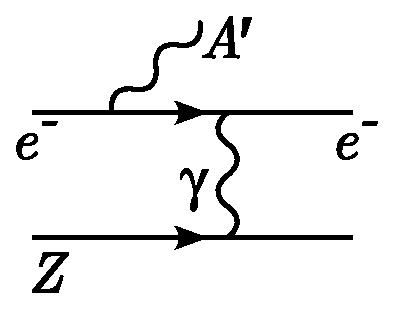
\includegraphics[width=.55\linewidth]{images/illustrative/aprime-photoprod.eps}
    \caption{Фоторождение $A'$ на ядре $Z$}
    \label{fig:aprime-production}
\end{figure}
%\end{wrapfigure}

Постулируя, что $a$ является псевдоскалярной частицей, можно построить 
феноменологический лагранжиан, описывающий его свободное движение и взаимодействие 
с электромагнитным полем 
\begin{equation}
    \mathcal{L}_{F+a} = - \frac{1}{4} g_{a \gamma \gamma} a F_{\mu \nu} \tilde F_{\mu \nu}
        + \frac{1}{2} (\partial_{\mu} a)^2 - \frac{1}{2} m^2_a a^2,
\end{equation}
где $\tilde{F}_{\mu \nu} = \frac{1}{2} \epsilon_{\mu \nu \lambda \rho} F^{\lambda \rho}$ --- дуальный тензор электромагнитного поля,
$g_{a \gamma \gamma}$ -- константа связи, и $m_a$ -- масса ALP частицы.

Эксперимент по поиску $a$ подразумевает постановку схожую с экспериментом
по поиску $A'$. Диаграмма реакций приведена на рисунке~\ref{fig:axion-photo}.

\begin{figure}[ht]
    \centering
    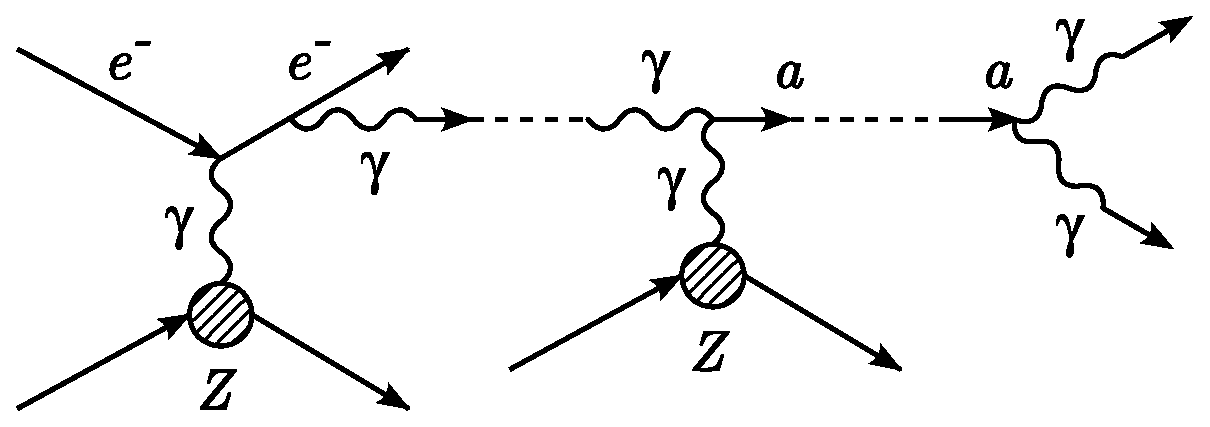
\includegraphics[width=0.75\linewidth]{images/illustrative/ALPs-photoprod-ours.eps}
    \caption{Фоторождение и распад аксион-подобной частицы (ALP).}
    \label{fig:axion-photo}
\end{figure}
\section{Оценки выхода сигнальных процессов}



В последние десятилетия, среди методов оценки физических эффектов вызванных
прохождением ионизирующего излучения через вещество, получил широкое применение
метод прямого численного моделирования, опирающийся на развитую теорию
методов Монте-Карло.
%TODO: citations

Учёт разнообразных параметров установки (геометрия детекторов, материалы
активных и пассивных частей детекторов) позволяет, в принципе, произвести
моделирование отклика детектирующей системы на фоновые и сигнальные события с
достаточно высокой степенью правдоподобности. Чаще всего экспериментальные
коллаборации располагают набором параметров свойственных определённому
энергетическому диапазону определяющему вполне феноменологию эксперимента,
в рамках которого уточнение и верификация модели производятся итеративно.
Учитываемые физические
процессы и явления при этом по большей части полностью включены в физику
Стандартной модели, и имеют к тому времени заранее определённые области
правдоподобия, определяемые энергией и составом излучения.

В случае исследования новых физических процессов, сложно поддающихся численному
моделированию или вовсе не включённых в Стандартную модель, практический
интерес представляет построение соответствующих генераторов событий (в рамках
методов Монте-Карло): такие программы позволяют произвести моделирование
сигнальных событий как совместно с фоновыми, для оценки параметров установки
(аксептанса, эффективности), так и отдельно, с целью выявления неочевидных
систематических эффектов, сделать достоверные предположения о характере отклика
детекторной системы и получить важные численные оценки для параметров
считывающей аппаратуры и статистики данных.

\subsection{Рождение тёмного фотона в толстой мишени}

Рассмотрим процесс испускания массивной $U(1)'$-частицы $A'$ в конечном или
начальном состоянии электроном рассеивающимся на ядре $Z$. С эффективной точки
зрения, $A'$ удобно рассматривать как эквивалент кванта тормозного излучения
с каплингом к электрону $e \epsilon$ вместо $e$ и массой $m_{A'}$.
Дифференциальное сечение, согласно предполагаемой кинематической картине,
может быть получено в модификации метода Вайтцзаккера-Вильямса выполненной
Кимом и Цаем \cite{KimTsaiWWReview}, через факторизацию на эффективный фотонный
поток, предложенную теми же авторами в 1986 г. в качестве модели для
аналогичного процесса с аксионом в конечном состоянии \cite{tsai.axion}.
В 1924 году Ферми предложил~\cite{Fermi1924}
способ быстрой оценки, который в 1934 году был развит Вайцзеккером и
(независимо) Вильямсом~\cite{Weizsacker1934, Williams1934} показавшим, что для налетающей частицы обладающей массой $M$,
зарядом $Ze$ и энергией $E=\gamma M$ справедливо приближение т.н. эквивалентных
(виртуальных) фотонов со спектральной плотностью $\rho (\omega)$:

\begin{equation}
    \rho ( \omega ) = \frac{Z^2 \alpha}{\pi \omega} ( 2 x K_0 (x) K_1 (x) - x^2 [K_1^2(x) - K_0^2(x) ] ),
    \label{eq:WWSpectrum}
\end{equation}
где $\omega$ соответствует эффективной энергии фотона,
$x = \omega b_{min} / \gamma$ -- минимальный прицельный параметр а
$K_0$, $K_1$ -- функции Бесселя. Можно видеть, что в релятивистском случае
($ x \ll 1 $) это выражение переходит в следующую форму
\begin{equation}
    \rho (\omega) \simeq \frac{Z^2 \alpha}{\pi \omega} \ln(\frac{1.123 \gamma}{\omega b_{min}} - 1/2).
\end{equation}

% TODO: не составит труда построить график этого распределения, которое имеет
% некоторое значение при качественной интерпретации результатов в дальнейшем

На основании этой аппроксимации
в работе \cite{bjorken} предлагается следующая оценка
дифференциального сечения примесного
фоторождения $A'$ \footnote{Некоторые соотношения в работе \cite{bjorken}
посчитаны с незначительными арифметическими ошибками, исправленные
соотношения см. в \cite{andreas2012}.}:
\begin{equation}
    \frac{1}{E^2_0} \frac{ d \sigma_{3 \rightarrow 2}}{d x d \cos{\theta_{A'}}} =
(8 \alpha \epsilon^2 \chi \beta_{A'}^2) \left[
    \frac{ 1 - x + x^2/2 }{U^2} + 
    \frac{ (1-x)^2 m^2_{A'} }{U^4} \cdot
        ( m^2_{A'} - \frac{U x}{1 - x} )
        \frac{}{}
\right],
    \label{eq:bjorkenCS}
\end{equation}
где $x = E_0/E_{A'} \in (m_{A'}/E_0, 1 - m_{A'}/E_0)$ -- относительная энергия
$A'$, $\theta_{A'} \in [0, \pi]$ -- угол вылета, относительная скорость
$\beta = \sqrt{ 1 - m_{A'}/E_0 }$, и
$U = (E_0 \theta_{A'} )^2 x + m^2_{A'} (1-x)/x + m_e^2 x$.
Эффективный поток фотонов $\chi$ даётся интегральным выражением:
\begin{equation}
\chi = \int_{t_{min}}^{t_{max}} d t \frac{t - t_{min}}{t^2} G_2 (t),
\label{eq:photoFlux}
\end{equation}
где $G_2(t) = G_{2, el} + G_{2, inel}$ -- общий электромагнитный форм-фактор
введённый в работе \cite{KimTsaiWWReview} как набор простых параметризаций
дающих хорошее количественное согласие (3\%) в описании эффекта тормозного
излучения.
% TODO: Детально влияние форм-фактора будет учтено в ч.
%Последуем пока рекомендации работы \cite{bjorken} с тем чтобы получить
%предварительную оценку 

При $m_{A'} \rightarrow 0$ переходит в классическое сечение тормозного
излучения, см. напр. \cite{bremsref}.

Выражение \eqref{eq:bjorkenCS} можно
проинтегрировать численно, с тем чтобы получить оценку полного
сечения образования $A'$, необходимую для реализации генератора событий.

\begin{figure}
    \centering
    %\includegraphics[scale=2]{chi-over-Z2.eps}
    % GNUPLOT: LaTeX picture with Postscript
\begingroup
  \makeatletter
  \providecommand\color[2][]{%
    \GenericError{(gnuplot) \space\space\space\@spaces}{%
      Package color not loaded in conjunction with
      terminal option `colourtext'%
    }{See the gnuplot documentation for explanation.%
    }{Either use 'blacktext' in gnuplot or load the package
      color.sty in LaTeX.}%
    \renewcommand\color[2][]{}%
  }%
  \providecommand\includegraphics[2][]{%
    \GenericError{(gnuplot) \space\space\space\@spaces}{%
      Package graphicx or graphics not loaded%
    }{See the gnuplot documentation for explanation.%
    }{The gnuplot epslatex terminal needs graphicx.sty or graphics.sty.}%
    \renewcommand\includegraphics[2][]{}%
  }%
  \providecommand\rotatebox[2]{#2}%
  \@ifundefined{ifGPcolor}{%
    \newif\ifGPcolor
    \GPcolorfalse
  }{}%
  \@ifundefined{ifGPblacktext}{%
    \newif\ifGPblacktext
    \GPblacktexttrue
  }{}%
  % define a \g@addto@macro without @ in the name:
  \let\gplgaddtomacro\g@addto@macro
  % define empty templates for all commands taking text:
  \gdef\gplbacktext{}%
  \gdef\gplfronttext{}%
  \makeatother
  \ifGPblacktext
    % no textcolor at all
    \def\colorrgb#1{}%
    \def\colorgray#1{}%
  \else
    % gray or color?
    \ifGPcolor
      \def\colorrgb#1{\color[rgb]{#1}}%
      \def\colorgray#1{\color[gray]{#1}}%
      \expandafter\def\csname LTw\endcsname{\color{white}}%
      \expandafter\def\csname LTb\endcsname{\color{black}}%
      \expandafter\def\csname LTa\endcsname{\color{black}}%
      \expandafter\def\csname LT0\endcsname{\color[rgb]{1,0,0}}%
      \expandafter\def\csname LT1\endcsname{\color[rgb]{0,1,0}}%
      \expandafter\def\csname LT2\endcsname{\color[rgb]{0,0,1}}%
      \expandafter\def\csname LT3\endcsname{\color[rgb]{1,0,1}}%
      \expandafter\def\csname LT4\endcsname{\color[rgb]{0,1,1}}%
      \expandafter\def\csname LT5\endcsname{\color[rgb]{1,1,0}}%
      \expandafter\def\csname LT6\endcsname{\color[rgb]{0,0,0}}%
      \expandafter\def\csname LT7\endcsname{\color[rgb]{1,0.3,0}}%
      \expandafter\def\csname LT8\endcsname{\color[rgb]{0.5,0.5,0.5}}%
    \else
      % gray
      \def\colorrgb#1{\color{black}}%
      \def\colorgray#1{\color[gray]{#1}}%
      \expandafter\def\csname LTw\endcsname{\color{white}}%
      \expandafter\def\csname LTb\endcsname{\color{black}}%
      \expandafter\def\csname LTa\endcsname{\color{black}}%
      \expandafter\def\csname LT0\endcsname{\color{black}}%
      \expandafter\def\csname LT1\endcsname{\color{black}}%
      \expandafter\def\csname LT2\endcsname{\color{black}}%
      \expandafter\def\csname LT3\endcsname{\color{black}}%
      \expandafter\def\csname LT4\endcsname{\color{black}}%
      \expandafter\def\csname LT5\endcsname{\color{black}}%
      \expandafter\def\csname LT6\endcsname{\color{black}}%
      \expandafter\def\csname LT7\endcsname{\color{black}}%
      \expandafter\def\csname LT8\endcsname{\color{black}}%
    \fi
  \fi
    \setlength{\unitlength}{0.0500bp}%
    \ifx\gptboxheight\undefined%
      \newlength{\gptboxheight}%
      \newlength{\gptboxwidth}%
      \newsavebox{\gptboxtext}%
    \fi%
    \setlength{\fboxrule}{0.5pt}%
    \setlength{\fboxsep}{1pt}%
\begin{picture}(8784.00,4320.00)%
    \gplgaddtomacro\gplbacktext{%
      \csname LTb\endcsname%
      \put(814,704){\makebox(0,0)[r]{\strut{}$0.1$}}%
      \put(814,1946){\makebox(0,0)[r]{\strut{}$1$}}%
      \put(814,3187){\makebox(0,0)[r]{\strut{}$10$}}%
      \put(946,484){\makebox(0,0){\strut{}$0.001$}}%
      \put(2806,484){\makebox(0,0){\strut{}$0.01$}}%
      \put(4667,484){\makebox(0,0){\strut{}$0.1$}}%
      \put(6527,484){\makebox(0,0){\strut{}$1$}}%
      \put(8387,484){\makebox(0,0){\strut{}$10$}}%
    }%
    \gplgaddtomacro\gplfronttext{%
      \csname LTb\endcsname%
      \put(176,2379){\rotatebox{-270}{\makebox(0,0){\strut{}$\chi/Z^2$}}}%
      \put(4666,154){\makebox(0,0){\strut{}$m_{A'}$, ГэВ}}%
      \put(7400,3882){\makebox(0,0)[r]{\strut{}W, 200 МэВ}}%
      \put(7400,3662){\makebox(0,0)[r]{\strut{}W, 1 ГэВ}}%
      \put(7400,3442){\makebox(0,0)[r]{\strut{}W, 6 ГэВ}}%
      \put(7400,3222){\makebox(0,0)[r]{\strut{}Al, 6 ГэВ}}%
      \put(7400,3002){\makebox(0,0)[r]{\strut{}Pb, 80 ГэВ}}%
    }%
    \gplbacktext
    \put(0,0){\includegraphics{images/aprime-generator/chi-over-Z2.eps}}%
    \gplfronttext
  \end{picture}%
\endgroup

    \caption{ Эффективный поток фотонов отнесённый к квадрату зарядового числа
$\chi/Z^2$ для различных материалов и энергий налетающей частицы: приведён
расчёт в соответствии с формулой \eqref{eq:photoFlux} для вольфрама и алюминия
(ср. с \cite{bjorken}) и свинца. Последний используется в качестве материала
активной мишени NA64. }
\end{figure}

% Эти графики сечений скучны и нерепрезентативны, так что смысла приводить их
% я не вижу. Возможно, будет целессобразно вынести их в приложение...
%\begin{table}[ht]
%  \centering
%  \begin{tabular}{c@{\quad}cc}
%                   & $E_0 = 5$ ГэВ & $E_0 = 80$ ГэВ \\
%       $m_A=5$ МэВ & \input images/ww-cs-plots/0.005_5
%                   & poison \\ \\
%    $m_A=16.7$ МэВ & \input images/ww-cs-plots/0.0167_5
%                   & \input images/ww-cs-plots/0.0167_80 \\ \\
%     $m_A=500$ МэВ & \input images/ww-cs-plots/0.5_5
%                   & \input images/ww-cs-plots/0.5_80
%  \end{tabular}
%  \caption{This is a caption.}\label{figtab}
%\end{table}

%TODO: более подробно раскрыть смысл \chi, G_1, G_2, etc.

%Для практической реализации генератора событий важно, что энергия инициирующей
%частицы (в статье рассмотрены электроны), вообще говоря, входит в формулу
%как параметр. Это значит, что при разыгрывании событий в ливне форм‐фактор
%должен быть рассчитан для каждого значения энергии электрона.

%Поскольку у функции дифференциального сечения есть особенность при
%$x \rightarrow 1$ и $\theta_{A'} \rightarrow 0$, а так же сделанные в статье
%\cite{bjorken} допущения ведут к ошибке в области больших импульсов, реализация
%генератора на основе сечения \eqref{eq:bjorkenCS} представляет существенную
%техническую трудность.

Из-за релятивистского характера кинематики, появившийся $A'$ в основном полетит
под малым углом к инициирующей частице ($\theta_{A'} \rightarrow 0$). Кроме
того, прямым следствием кинематической картины является то что $A'$ в подавляющем
большинстве случаев приобретает большой импульс ($x \rightarrow 1$).

%Взаимодействия в
%конечном состоянии, если я правильно понимаю дело, происходить не будет,
%что изрядно облегчает задачу встраивания процесса в Geant4. В терминах
%объектов API Geant4 процесс будет выражаться в изменении кинематических
%характеристик инициирующей частицы и появлении новой частицы ($A'$). Всякое
%прочее взаимодействие инициирующей частицы с веществом — независимые
%процессы по отношению к примесному рождению $A'$, и, таким образом, могут
%быть разыграны отдельно.

%В статье так же есть готовые
%калибровочные оценки на тонкой мишени, благодаря которым возможно оценить
%согласие написанного генератора с теоретическим ожиданием (см. Appendix B).

Важно заметить, что $A'$ может каскадно распадаться на <<видимые>> частицы.
Помимо регистрации событий по недостающей энергии (<<невидимый>> канал),
эксперимент NA64 предполагает анализ и видимой моды излучения. С точки
зрения Монте‐Карло моделирования процессы примесного фотообразования и
последующего распада независимы и должны быть реализованы раздельно,
путём реализации независимых интерфейсов процессов.

%\begin{figure}
%    \centering
%    %\includegraphics[scale=2]{chi-over-Z2.eps}
%    \input images/ww-cs-plots/0.005_80
%    \caption{ Дифференциальное сечение для различных масс и энергий электрона. }
%\end{figure}

% TODO: сравнение результатов численного интегрирования дифференциального
% сечения и оценки полного, согласно статье показывает существенную
% систематическую разницу: относительно аналитической оценки, численный
% результат оказывается меньше на фактор 3.78e-5/E_0. Это говорит либо о
% неверной формуле для дифференциального или полного сечений, данной в статье,
% либо об упущенных сомножителях. Необходимо проверить кинематическое
% рассмотрение.
% см.: assets/generator/cs
% gnuplot> plot 'cs-est-vs-num.dat' u 1:2 w linespoints title 'estimation', 'cs-est-vs-num.dat' u 1:($3*3.78e-5/$1) w linespoints title 'full CS'

\subsection{Мажоранта для генерации событий}

Рассмотрим сечение \eqref{eq:bjorkenCS} с точки зрения задачи
построения генератора событий, актуальной в приложениях. С точностью до
нормировки, функция плотности вероятности отвечающая сечению определяется
следующим множителем:

\begin{equation}
    f_{var}(x, \theta) = x \sin \theta \frac{1-x}{U^2} \left[
        1 + (1-x)^2 + \frac{ 2 (1-x)^2 m_{A'}^2 }{U^2} \left( m_{A'}^2 - \frac{U x}{1-x} \right)
        \right]
\label{eq:bjorkenVarPDF}
\end{equation}

Наиболее простым в реализации, но зачастую малоэффективным методом для
генерирования значений в соответствии с заданной функции плотности
вероятности $f(x_i)$ является т.н. \emph{метод accept/reject}, который
предполагает совместное разыгрывание $N+1$ случайных
чисел $\{\tilde{x}_i, \tilde{x}_{N+1}\}, i = 1, 2, \dots, N+1$. Разыгранным в
соответствии с заданным распределением считается вектор $\tilde{x}_i$ для
которого $x_{N+1} \le f(\tilde{x}_i)$. Наиболее общая реализация
предполагает, что $\{\tilde{x}_i, \tilde{x}_{N+1}\}$ распределены равномерно.

Наиболее точным и вычислительно-эффективным методом является
т.н. \emph{метод обратной функции}, в котором случайное значение $\tilde{x}$ получается
путём подстановки некоторого равномерно-распределённого случайного значения в
функциональное уравнение
\begin{equation}
    u = \int\limits_{-\infty}^{\tilde{x}} f(x) \dd{x}.
\label{eq:revertFuncIntEq}
\end{equation}

В тех случая когда удаётся алгебраически разрешить уравнение
\eqref{eq:revertFuncIntEq}, решение обозначают символически
как~$F^{-1}(u) = \tilde{x}$,~---~собственно, обратную функцию.

\begin{comment}
Другим, достаточно популярным методом генерирования значений по заданному
закону распределения, является подход использующий свойства цепей
Маркова~(напр. алгоритм Метрополиса-Гастингса, алгоритм Гиббса и т.д.). Этот
подход, в сравнении с методом обратной
функции может быть достаточно хорошо обобщён, но он связан с усложнением
технической реализации, поскольку алгоритмы основанные на нём предполагают
определённое число предварительных итераций, прежде чем получаемые числа
оказываются распределены достаточно независимо. Кроме того, метод обратной
функции позволяет естественную параметризацию физическими величинами входящими
в дифференциальное сечение, в то время как использование цепей Маркова
потребовало бы создания отдельных вычислительных состояний для каждого набора
параметров. Последнее обстоятельство достаточно важно в задачах моделирования
излучения с непрерывным спектром.
\end{comment}

Отыскание $F^{-1}(u)$ для \eqref{eq:bjorkenCS}
затруднено, поскольку потребует решения
трансцендентного уравнения вида $a x^2 + b x + c = \arctanh x$, однако можно
воспользоваться модифицированным методом accet/reject (метод фон Неймана
\cite{vonNeumannVarTechs}.
Если подобрать мажорирующую функцию, которая, с одной стороны, окажется не
меньше $f_{var}(x, \theta)$ во всей области определения, с другой ---
будет достаточно близка к ней с тем чтобы уменьшить долю отклонённых
случайных значений.


Выбор функции целесообразно произвести руководствуясь простыми алгебраическими
соображениями, упрощая аналитический вид исходной функции с тем чтобы получить
верхнюю оценку соответствующих слагаемых и множителей.

Запишем \eqref{eq:bjorkenVarPDF} в следующем виде:
\begin{equation}
    f_{var}(x, \theta) = \frac{x \sin \theta}{2 U^2} \left[
        1 - x + \frac{x^2}{2}
        + \frac{m_{A'}^4 (1-x)^2}{U^2}
        - \frac{m_{A'}^2 x (1-x)}{U}
        \right],
\end{equation}
где полином $x^2/2 - x + 1 \le 1, x \in [0,1]$, а для оставшихся слагаемых в
квадратных скобках справедливо:

\begin{equation}
    \frac{m_{A'}^4 (1-x)^2}{U^2} - \frac{m_{A'}^2 x (1-x)}{U} =
    - \frac{m_{A'}^2 x (1-x)^2 (E_0^2 \theta^2 x + m_e^2 x) }{U^2} \le 0,
\end{equation}
то есть:
\begin{equation}
    f_{var}(x, \theta) \le \frac{x \sin \theta}{2 U^2}.
\end{equation}

Для построения генераторов понадобится интегрировать мажоранту, и чтобы
упростить эту процедуру удобно воспользоваться тем что $\sin \theta \le \theta$.
Нужно заметить, что поскольку большинство событий сосредоточено в области
малых $\theta$, где
$\sin \theta \sim \theta$, подобное упрощение не приведёт к значительному
увеличению доли отклонённых случайных значений в численной процедуре.

Тогда для генерации
кинематических переменных в дальнейшем, там где упоминается моделирование в
приближении эквивалентных фотонов, в качестве плотности распределения исходных
(по отношению к алгоритму "accept/reject") параметров будем использовать функцию
\begin{equation}
    \mu_1(x, \theta) = x^3 \theta
        (E_0^2 \theta^2 x^2 + m_{A'}^2(1-x) + m_e^2 x^2)^{-2}.
\label{eq:majorant1}
\end{equation}

\begin{figure}
    \centering
    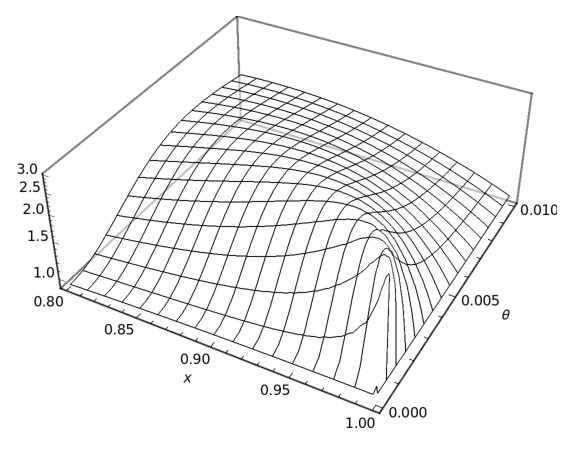
\includegraphics[scale=1]{rel-err-mj1.eps}
    %\input assets/plots/rel-err-mj1
    \caption{ Характерный вид относительной ошибки при
    аппроксимации~$f_{var}(x, \theta)$ мажорантой~$\mu_1(x,\theta)$. }
    \label{fig:mj1RelError}
\end{figure}

На рис. \ref{fig:mj1RelError} показан график относительной
ошибки $(\mu_1(x,\theta) - f(x,\theta)/f(x,\theta)$.
Относительная ошибка квадратично возрастает в области больших $\theta$, в
зависимости от $m_{A'}$ и $E_0$ достигая двух порядков величины аппроксимирующей
функции. Однако, при практическом использовании \eqref{eq:majorant1}
для генерирования значений $\tilde{x}$ необходимо иметь в виду то
обстоятельство, что большинство событий эмиссии $A'$ будут
сосредоточены в кинематической области $x \rightarrow 1, \theta \rightarrow 0$,
где $\mu_1(x, \theta)$ сравнительно точно воспроизводит поверхность
\eqref{eq:bjorkenCS}.

Первообразная по $\theta$ к ней имеет достаточно простой вид, удобный для
дальнейших преобразований:
\begin{equation}
    M_1(x) = \int \mu_1(x, \theta) \dd{\theta} = x / (2 E_0 \left[m_{A'}^2 (1 - x) - x^2 (m_e^2 + E_0^2 \theta^2) \right]).
\end{equation}

Тогда обратная функция на переменную $\theta$ через параметр $x$ и некоторое
равномерно распределённое случайное число $u \in [0, 1]$ получается
аналитически. С учётом нормировки
(для масштабных преобразований важно выдерживать относительный масштаб функций
$f_{var}(x, \theta)$ и $\mu(x, \theta)$):
\begin{equation}
    \theta^2 (u, x) = \pi^2 u \frac{ (x-1) + \frac{m_{e}^2}{m_{A'}^2} x^2 }
              { (x-1) + (\frac{m_{e}^2}{m_{A'}^2} - \pi^2 \frac{E_0^2}{m_{A'}} (1-u)) x^2 }.
    \label{eq:thetaExpr}
\end{equation}

Проинтегрировать
%$\int\limits_0^{\tilde{x}} \mu(x, \theta) d x$
$M_1(x)$
второй раз достаточно просто, однако
чтобы затем выразить переменный верхний предел понадобится разрешать
трансцендентное уравнение. Это можно либо сделать численно, либо
воспользоваться значениями $\vardbtilde{x}$ разыгранными в соответствии с той
же техникой.

\begin{figure}
    \centering
    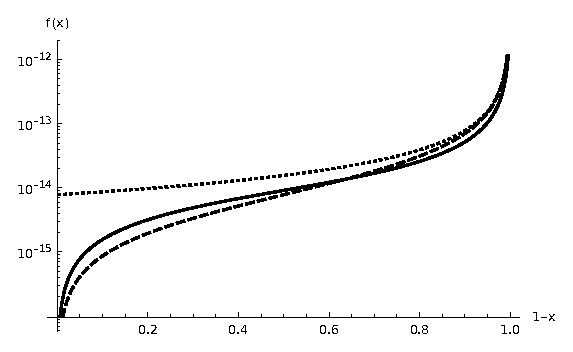
\includegraphics[scale=1]{mj1-mj2.eps}
    %\input assets/plots/rel-err-mj1
    \caption{ Характерный вид кривых, с точностью до нормирующей константы,
    соответствующих $M_1(x)$ (сплошная линия),
    $\mu_2(x)$~(короткий штрих)
    и аналитической аппроксимации интегрального по $\theta$ сечения
    $\dd{\sigma}/\dd{x}$ из \cite{bjorken}.}
    \label{fig:mj1mj2}
\end{figure}

Для этого запишем мажоранту $\mu_2(x)$ в виде:
\begin{equation}
    \mu_2(x) = ( 2 E_0^2 (m_{A'}^2 (1 - x) + m_e^2 x ) )^{-1},
\end{equation}
и получим следующие алгебраические результаты, необходимые для
разыгрывания~$x$:
\begin{align}
    M_2 = \int \mu_2(x) \dd{x} =& \frac{1}{2 E_0^2} \frac{\ln{( m_{A'}^2 (1 - x) + m_e^2 x )}}{(m_e^2 - m_{A'}^2)}, \\
    \vardbtilde{x}(u) =& \frac{1}{2 E_0^2} \frac{1-(m_e/m_{A'})^{2 u}}{1-(m_e/m_{A'})^{2}}.
    \label{eq:mj2x}
\end{align}

$M_2(x)$ упрощает поведение функции плотности вероятности
для $x$ в районе небольших переданных импульсов (см.
рис~\ref{fig:mj1mj2}), что, с учётом
относительной вероятности процесса не является важным для задач моделирования
эмиссии $A'$.

Таким образом, алгоритм получения набора случайных
чисел $\{x,\theta\}$ отвечающих плотности распределения
заданной дифференциальным сечением \eqref{eq:bjorkenCS}, сводится к следующей
последовательности операций:
\begin{enumerate}
    \item Разыграть пару равномерно распределённых в интервале $[0,1]$
        случайных чисел $\{u_1, u_2\}$. Подстановкой $u_1$ в \eqref{eq:mj2x}
        получить $\vardbtilde{x}$. Повторять до тех пор,
        пока для какой-то пары не окажется,
        что $u_2 \cdot \mu_2(\vardbtilde{x}) \le M_1 (\vardbtilde{x})$, ---
        отвечающий этому условию $\vardbtilde{x}$ следует принять за
        $\tilde{x}$.
    \item Разыграть пару равномерно распределённых в интервале $[0,1]$
        случайных чисел $\{u_3, u_4\}$. Подстановкой $u_3$ и $\tilde{x}$
        в \eqref{eq:thetaExpr} получить $\tilde{\theta}$. Если оказывается,
        что $u_4 M_1(\tilde{x}, \tilde{\theta}) > f_{var}(\tilde{x}, \tilde{\theta})$,
        необходимо повторить процедуру с п.1.
\end{enumerate}

Прошедшие процедуру псевдослучайные $\tilde{x}$ и $\tilde{\theta}$
соответствуют относительной энергии и полярному углу эмиссии $A'$ в приближении
Вайцзеккера-Вильямса, и могут использоваться при симуляциях методами
Монте-Карло. Описанный метод обладает тем важным преимуществом, что все
основные соотношения естественно параметризуются $E_0$ и не требуют дорогих
вычислений для разыгрывания во всём непрерывном спектре электромагнитного
ливня.


\begin{comment}
Выражение спектра \eqref{eq:WWSpectrum} получило широкое распространение для
описания однофотонных процессов. Однако это
приближение демонстрирует существенное расхождение в эффектах связанных со
значительным влиянием форм-факторов учитывающих распределение зарядовой
плотности в рассеивающих центрах. В работе
\cite{KimTsaiWWReview} Ким и Цай (Tsai) предлагают использовать
модифицированный метод Вайцзеккера-Вильямса для оценки дифференциальных сечений
в реакциях фотообразования аксионов на ядре, с учётом форм-факторов
ответственных за упругое и неупругое взаимодействие.
%Метод был верифицирован
%на основании точных значений дифференциальных сечений измеренных в \cite{}. slac-pub-1105 -- not found
Для целей настоящей работы
интерес представляет затем статья \cite{tsai.axion} в которой Цай
применяет авторский метод для получения количественных оценок выхода аксионов в
реакциях рассеяния тяжёлых ионов (измерения на спектрометре
EPOS~\cite{cowan.positron.1985}), --- соответствующий механизм назван
<<аксионным тормозным излучением>> (англ. \emph{axion bremsstrahlung})
и описывается диаграмой \ref{TODO}, где
%$P_1$, $P_2$, $P_i$, $P_f$ и $k$, ---
$k$ и $k'$, $p$ и $p'$ и $q$, ---
4-импульсы налетающего и рассеянного электронов, рассеивающего центра в
начальном и конечном состоянии (рассматривается в т.ч. и неупругое
взаимодействие) и аксиона, соответственно.

Оригинальную формулу работы \cite{KimTsaiWWReview}
\begin{equation}
    \left( \frac{d \sigma}{d \Omega d p} \right)_{WW} = \frac{\alpha^3}{2 \pi} \cdot
    \frac{E}{k - E} k t_{min}' ( - g_{\mu \nu} L^{\mu \nu} )_{t = t_{min}} \chi,
\end{equation}
в которой множитель $\chi$ получил название эффективного потока эквивалентных
фотонов:
\begin{equation}
    \chi = \frac{1}{2 M_i} \int\limits_{t_{min}}^{t_{max}} \frac{dt}{t^2} \int\limits_{M_i^2}^{(u-m)^2}
    d M_f^2 [(t - t_{min}) W_2 + 2 t_{min}' W_1],
\end{equation}
$M_f$ --- , $ M_i $ ---, $ L_{\mu \nu} $ ---, $g_{\mu \nu}$
% TODO: без спинов -- см ф-лу 3.17

Поскольку эти фотоны пространственноподобны, их виртуальность $t$ мала по
сравнению с прочими инвариантами задачи ($m_{A'}$), и взаимодействие электрона
с мишенью в основном определяется поперечной поляризацией. Таким образом,
кинематическое рассмотрение можно свести к задаче рассеяния на реальных фотонах
(комптоновское рассеяние, см. \cite{KimTsaiWWReview}):

\begin{equation}
\frac{d \sigma ( e(k) + Z(p) \rightarrow e(k') + A'(q) + Z(p') )}{ dE_{A'} d \cos \theta_{A'} } =
    \frac{ \alpha \chi }{ \pi } \frac{E_0 x \beta_{A'}}{1 - x} \frac{ d \sigma (p + q \rightarrow p' + k) }{d (p k)},
\end{equation}

где $x = E_{A'}/E_0$, $t = - q^2$, $\beta_{A'} = \sqrt(1 - m_{A'}^2/E_0^2)$.

%В числе прочего обсуждается, что механизм Примакова пренебрежимо мал по вкладу
%по сравнению с тормозным.

% TODO: ...
\end{comment}

\subsection{Оценки выхода сигнального события}

Согласно выражению дифференциального сечения~\eqref{eq:bjorkenCS}
в работе~\cite{bjorken} приблизительное количество
образовавшихся~$A'$:
\begin{equation}
    N_{A'} \approx N_e C' \epsilon^2 \frac{m^2}{m^2_{A'}}, \quad C' \simeq 10.
    \label{eq:aprime-yield-approx}
\end{equation}

В постановке эксперимента важно учесть характерное время
жизни гипотетической частицы, поскольку распадной длины может
быть недостаточно для покидания активной мишени. Характерная
(средняя) длина распада согласно~\cite{bjorken}:
\begin{equation}
    l_0 \approx 0{,}8 \text{см} \cdot \frac{E_0 / 10 ~\text{ГэВ}}{N_{eff}}
        \left( \frac{10^{-4}}{\epsilon} \right)^2 \left( \frac{100~\text{МэВ}}{m_{A'}} \right)^2.
    \label{eq:aprime-decay-length}
\end{equation}

Выражения \eqref{eq:aprime-yield-approx} и \eqref{eq:aprime-decay-length}
позволяют грубо оценить примерный выход реакции в свинцовой мишени,
учитывая геометрические ограничения на длину мишени. Результаты
такой оценки выполненной для $\epsilon = 10^{-4}$ и $N_{e} = 10^{14}$ приведены в
таблице~\ref{tab:aprime-geom-yield-estimations}, где
$m_{A'}$ -- гипотетическая масса тёмного фотона,
$N_{prod}$ -- число родившихся $A'$ в толстой мишени ($C'\approx 10$),
$l_{1/2} = l_0 \text{ln}~2 \approx 0{,}693 ~ l_0$ -- длина
на которой распадается половина~$A'$,
$P_{dec}$ -- примерная доля распавшихся частиц при длине распадной базы
в $1~\mathrm{м}$,
$N_{obs}$ -- число наблюдаемых распадов ниже по пучку.

\begin{table}[h]
\centering
\begin{tabular}{r|ccccc}
 $m_{A'}$, ГэВ & $N_{prod}$ & $l_{1/2}$, см & $P_{dec}$ & $N_{obs}$ \\ \hline
$0{,}01$ & $261$        & $555$    &  $0{,}118$ & $30{,}7$ \\
 $0{,}1$ & $2{,}61$     & $5{,}5$  &  $1$       & $2{,}61$ \\
 $0{,}5$ & $0{,}104$    & $0{,}2$  &  $1$       & $0{,}104$ \\
     $1$ & $0{,}0261$   & $0{,}05$ &  $1$       & $0{,}0261$
\end{tabular}
\caption{Оценка согласно \eqref{eq:aprime-yield-approx} и \eqref{eq:aprime-decay-length}}
\label{tab:aprime-geom-yield-estimations}
\end{table}
%\begin{flushleft}
%\footnotesize\textit{Примечания.} (i) $N_{\rm prod}\approx N_e\,C'\,\varepsilon^2(m_e^2/m_{A'}^2)$, $C'\simeq 10$ (толстая мишень). (ii) $\ell_0\simeq 0.8~\mathrm{см}\cdot\frac{E_0/10~\mathrm{GeV}}{N_{\!eff}}\left(\frac{10^{-4}}{\varepsilon}\right)^2\!\left(\frac{100~\mathrm{MeV}}{m_{A'}}\right)^2$. (iii) Если распадной объём начинается \emph{после} экрана длиной $S$, используйте $P=e^{-S/\ell_0}\bigl(1-e^{-L/\ell_0}\bigr)$. (iv) При $m_{A'}\ge 2m_\mu$ разумно брать $N_{\!eff}\gtrsim 2$, что уменьшит $\ell_0$ и увеличит $P$.
%\end{flushleft}

Из таблицы~\ref{tab:aprime-geom-yield-estimations} видно, что установка
с толщиной активной мишени в несколько десятков сантиметров и распадной
базой порядка метра и более в состоянии зарегистрировать десятки
частиц с массами до сотни МэВ и константой связи более $10^{-4}$.

Более точные оценки чувствительности эксперимента для этой и других
теоретических моделей, включающие более точный учёт форм-фактора,
подробно изложены в работе~\cite{voronchihin2025}.

\section{Постановка эксперимента}

Эксперимент NA64 (а также его <<мюонная версия>>, получившая название
NA64mu) использует постановку <<\emph{active beam dump}>> в рамках
которой массивная мишень сама по себе является детектором, а в конкретном
случае NA64 -- гетерогенным (свинец-полиметилметакрилат) электромагнитным
калориметром высокой гранулярности ECAL.

\subsection{Описание установки}

Начатый в 2015-ом году, эксперимент NA64 изначально
был направлен на поиск лёгкого бозона $A'$ получившего в литературе название
<<\emph{тёмный фотон}>> из-за того что гипотетическим механизмом его
образования является редкая конверсия посредством механизма электромагнитного
смешивания, которую можно описать через соответствующую добавку к
электромагнитному слагаемому лагранжиана \acrshort{sm}.

Экспериментальная установка для поиска $A'$ по недостающей энергии
в упрощённом виде изображена на рисунке \ref{fig:setup-schematic-invis}.
Установка состоит из двух калориметров -- электромагнитного
гетерогенного (сэмплирующего) калориметра ECAL, играющего роль активной мишени,
и адронного гетерогенного
калориметра HCAL. Установка снабжена системой мечения частиц, состоящей из
двухплечевого спектрометра на основе газовых микроструктурных трековых
детекторов T1-T4, измеряющих отклонение электронов в поле
магнита~($1.5\text{Тл}$). Триггерная система в простейшем случае
состоит из телескопа быстрых сцинтилляционных счётчиков S1, S2, S3.
Вето-детектор V1 и мюонный счётчик MU1 включаются в триггер в
режиме антисовпадений для исключения гало пучка и подавления мюонного
фона.

\begin{figure}
    \centering
    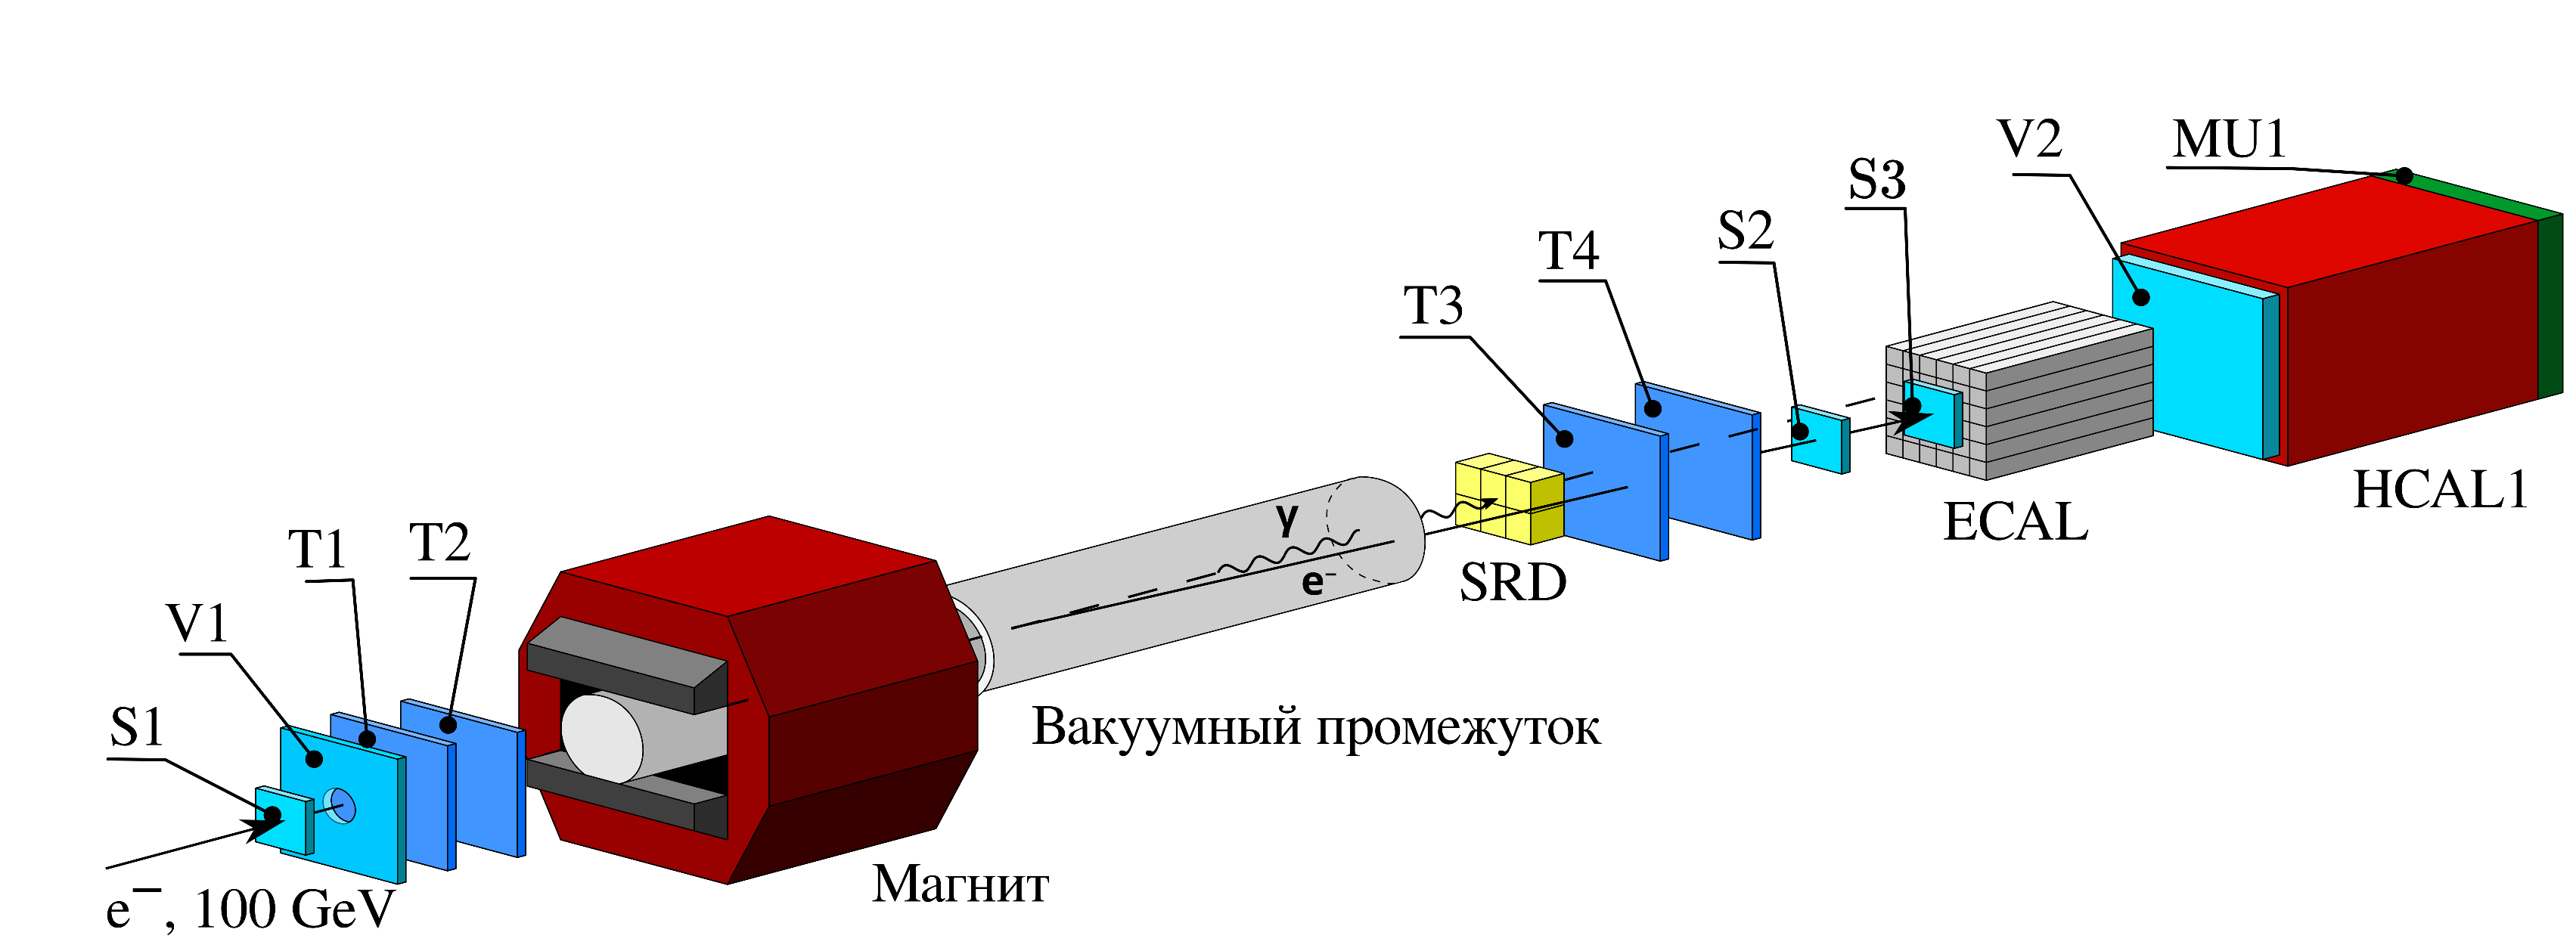
\includegraphics[width=1\linewidth]{images/illustrative/setup-schematic.eps}
    \caption{Размещение детекторов установки NA64 в постановке для обнаружения невидимых частиц}
    \label{fig:setup-schematic-invis}
\end{figure}

Поиск по недостающей энергии заключается в регистрации таких событий,
когда в обоих калориметрах отсутствует существенная часть энергии
инициирующей частицы (несколько десятков ГэВ), что соответствует
образованию высокоэнергетической частицы, способной покинуть
установку без взаимодействия.

Нужно заметить, что ряд процессов \acrshort{sm} в теории способны
реализовать такую сигнатуру: т.н. проникающие (<<пробивные>>,
англ. \emph{punchthrough}) фотоны, нейтральные частицы, мюоны,
альбедо-рассеяние частиц в первых нескольких актах взаимодействия в
мишени и т.д. NA64 оценивает вероятность таких событий менее $10^{-12}$,
что определяет нижний порог чувствительности установки к реакциям такого
типа.

Изображённая на рисунке~\ref{fig:setup-schematic-invis} постановка
может быть существенно модифицирована. Например, с целью подавления фоновых
каналов вместо сцинтилляционного детектора V1 для исключения
адронной компоненты фона в эксперимент в 2018г. были введены сэмплирующие
медные вето-калориметры, трекер дополнен несколькими дополнительными
микропаттерными детекторами и трубчатыми дрейфовыми
детекторами~(\emph{straw}-станциями). Для оценки мюонных фонов
straw-станции низкого разрешения расположены позади адронного калориметра.
В реальности, калориметр HCAL имеет продольную сегментацию, и состоит из
четырёх независимых модулей с поперечной сегментацией $3\times 3$ для
приближённой оценки профиля адронного ливня.

В качестве детектора синхротронного излучения (SRD) в разное время применялись
сегментированные калориметры BGO (из германата висмута), LYSO (ортосиликат
лютеция легированный церием), а так же вольфрам-пластиковые ячейки близкие
по составу к элементам электромагнитного калориметра ECAL.

% TODO: ECAL radiation length
% In order to measure direction of e/m shower and provide good \pi_0 rejection
% (why?) a preshower detector would be required at CMS --- shashlik proposal
% 1993
% TODO: HCAL radiation length

\subsection{Получение пучков и номенклатура данных}

Источником пучка выосокэнергетических ($100~\text{ГэВ}$) электронов в
эксперименте NA64 является ускоритель SPS (\emph{Super Proton
Synchrotron} – протонный суперсинхротрон). Вокруг ускорителя расположены
несколько экспериментальных зон. Эксперимент NA64 проводится в
Северной зоне (\emph{North Area}), включающей в себя два наземных
и один подземный залы, в которых размещены несколько станций вывода
пучка. На этих станциях пучок может выводиться напрямую в зону
эксперимента, либо направляться на мишень-конвертер для генерации пучка
вторичных частиц. Установка NA64 развёрнута на площадке H4,
предоставляющей электронный и адронные пучки. Для
реализации программы NA64mu, оборудование эксперимента перемещается на
площадку M2.

\subsubsection{Конверсия протонов пучка SPS}

В постановке на электронах NA64, пучок протонов с энергией $450~\text{ГэВ}$
интенсивностью $1{,}5 \times 10^{12}$ протонов/на период сбрасывается
на бериллиевую мишень, откуда пучок вторичных частиц передается в
тракт H4, состоящий из набора коллиматоров, отклоняющих и фокусирующих
магнитов, обеспечивающих малый разброс по энергиям и высокую чистоту пучка.

Первичная мишень представляет собой набор из пяти бериллиевых пластин
различной толщины. Толщины пластин составляют 40, 100, 180, 300 и 500~мм.
Пластины установлены в подвижном корпусе окруженном защитой. Соотношение
доли электронов к адронам в конверсионном ливне растет линейно с
увеличением длины мишени. Вторичные адроны образуются в реакциях вида
$p + Z \rightarrow H$ и их доля растёт в линейной пропорции к толщине
мишени $L$, в то время как вторичные электроны в основном являются результатом
распада адронов в реакциях
вида~$p + X \rightarrow \pi^0 \rightarrow \gamma \gamma$, где
аннигиляционные кванты $\gamma$ затем образуют в материале мишени
$e^{+}e^{-}$-пары. Часть из них, пропорциональная $e^{-L}$ поглощается
в веществе мишени. Таким образом, отношение полного выхода электронов и
адронов в конвертере пропорционально $L$ ($L^2 e^{-L}/L e^{-L} = L$),
что позволяет осуществлять эффективную конверсию и сепарацию вторичных
электронов в тракте H4.

Ускорительный комплекс SPS производит вывод пучка периодически --
с периодом в несколько десятков секунд (называемых \emph{суперциклом}),
в течение которых чередуются этапы накопления и сброса пучка.
Сброс пучка длится несколько секунд, остальное время происходит
накопление протонных сгустков в ускорительной ситсеме.

\subsubsection{Номенклатура данных}

К механизму накопления и сброса пучка ускорителя SPS привязана
идентификация событий в данных NA64.

Наиболее общей временной отметкой является отдельный
\emph{экспериментальный сеанс} в течение которого набор
детекторов установки и их взаимное геометрическое расположение
остаются в большой степени неизменными. В течение сеанса
процедуры настройки, калибровки и геометрической юстировки
детекторов производятся заново, обычно в несколько этапов.

С точки зрения накопленных данных, сеансы делятся на набор
пронумерованных подряд \emph{ранов} (англ.~\emph{run}) --
периодов набора статистики с типичной
продолжительностью в один или два часа, в течение которых
экспериментальный зал закрыт и условия набора данных предполагаются
постоянными. Номер рана остаётся уникальным в течение всего
жизненного цикла эксперимента.

Начало и конец рана выдерживаются привязанными к числу актов
сбросов пучка ускорителем. Временной интервал в течение которого
производится квазинепрерывный (банчированный) вывод пучка
называется~\emph{спилл}~(англ. \emph{spill}). Спиллы нумеруются
в ране подряд, и таким образом номер спилла в ране остаётся
уникальным.

Наконец, в пределах одного спилла, нумеруются подряд отдельные
события зарегистрированные триггером.

Таким образом, три числа обозначающие
\begin{itemize}
    \item Номер рана,
    \item Номер спилла,
    \item Номер события в спилле
\end{itemize}
составляют уникальный идентификатор события, который следует
использовать в программной базе эксперимента.

Ожидается, что число ранов NA64 не превысит $10^7$, число
спиллов в ране не превышает $10^3$, а число событий в одном
принципиально ограничено $10^9$. Таким образом, тип данных
для обозначения события потребует мощности в $10^19$ уникальных
значений, что позволяет кодировать идентификатор события
64-разрядным целым числом~($2^{64} \simeq1.85\times10^{19}$),
с сохранением семантики <<ран, спилл, номер события>>.

\section{Детекторы}

\subsection{Электромагнитный калориметр}

Оригинальная идея считывать свет из слоистого калориметра посредством
спектросмещающих волокон (WLS) предложена в 1985 году Фесслером \cite{Fessler-Shashlik-1985}.
Идея была впервые реализована в виде гетерогенного ячеистого калориметра в
1991-1992 годах в ИЯИ РАН для эксперимента E-865~(BNL, США) \cite{BADIER199474}.
% ^^^ проверить, впервые ли -- доклад Гущина (см. слайд №5) выглядит
% пристрастным: http://www.inr.troitsk.ru/rus/kud-sem/gushchin26-03-12.pdf
% Встречал упоминание о гетерогенном калориметре CDF (Fermilab), 1988, где
% при толщине 18 X_0 Pb/scint разрешение составляло 13.5%/\sqrt{E}
% KLOE использовали 15 X_0 с файберами в 1995 5.7%/\sqrt{E} + .6%
В последующие годы калориметры такого типа получили широкое распространение за
счёт ряда технологических преимуществ~\cite{grupenDetectors2008}.
К числу таких преимуществ относятся:
\begin{itemize}
    \item Возможность создания калориметра под необходимый мольеровский радиус,
    позволяющий производить пространственное разделение ливней от различных частиц, \item высокая радиационная стойкость, устойчивость отклика при работе в магнитном поле,
    \item стабильное энергетическое разрешение и высокая скорость отклика во
    многих случаях позволявшая включать такой калориметр в триггерную систему.
\end{itemize}

Идея нашла применение во многих экспериментах.
%:PHENIX (BNL), LHCb, DELPHI, CMS, COMPASS (CERN), HERA-B (DESY) и т.д.
С 1993 по 2003 годы в CERN действовала коллаборация посвящённая
развитию детекторов такого типа для задач эксперимента
CMS --- RD36~\cite{rd36-shashlik-1996}.
%Работы RD36 послужат методической основой для предлагаемой в
%настоящей диссертации процедуры калибровки ECAL \cite{rd36-shashlik-1996}.
% R&D proposal of 1993 https://cds.cern.ch/record/293003/files/SC00000220.pdf :
%   a = 8.4 +/- 1, c = .37 +/- .3, b = .8 +/- .2
%   \sigma_{mrad} = 70 / \sqrt{E}.
% 8.1  0.5  0.33

Калориметр NA64 представляет собой прямоугольный сегментированный блок, ячейки
которого конструктивно схожи с использованными в RD36 и COMPASS,
%ECAL NA64 имеет сегментацию, размеры ячеек, толщины слоёв и
%размещение оптического волокна.
Ячейки состоят из пластин свинца и
полиметилметакрилата (\acrshort{pmma})
набранных на стальные стержни для обеспечения механической
прочности с проходящим вдоль ячейки оптическим волокном имеющим оптический
контакт с пластинами сцинтиллятора.
Поперечная сегментация калориметра -- $6 \times 6$ или $5 \times 6$ квадратных
ячеек со стороной $38.2~\text{мм}$.
В продольном направлении калориметр разделён на предливневую и основную
части. На рисунке~\ref{fig:ecal-assembly-photo-opened} приведена фотография
торцевой части калориметра $6 \times 6$ в процессе установки светопроводящих
волокон, которые можно видеть в нижней части рисунка. торцы волокон от каждой
ячейки зачищаются и сводятся в пучок на катоде одного фотоприёмника.
\begin{figure}[h]
    \centering
    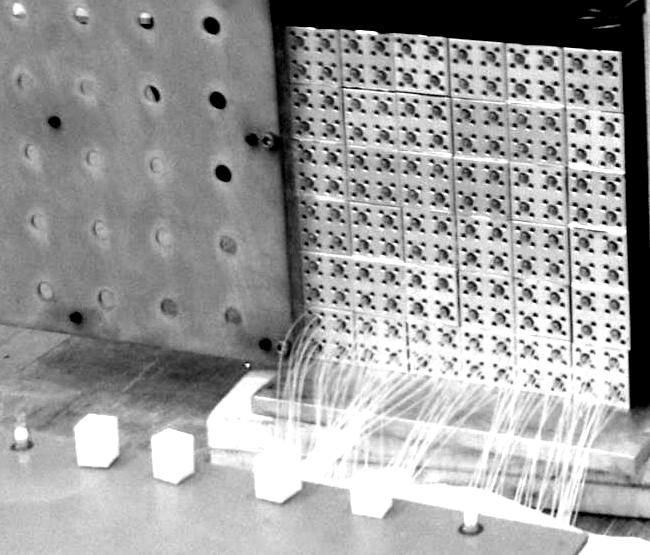
\includegraphics[width=0.5\linewidth]{images/illustrative/ecal-assembly-photo-opened.png}
    \caption{Фотография торцевой части ECAL NA64 со снятым кожухом}
    \label{fig:ecal-assembly-photo-opened}
\end{figure}
Свинцовые пластины имеют толщину~$1.5~\text{мм}$,
пластины из \acrshort{pmma} имеют толщину $1.55~\text{мм}$.
Для предохранения поверхности сцинтиллятора от механического
воздействия между ними вводится бумажная проставка толщиной $140~\text{мкм}$.
Предливневая часть состоит из 16-и слоёв, основная часть из 150-и.
Все пластины имеют перфорацию для пропускания светопроводящего волокна
(16 отверстий на ячейку) и армирующих стальных стержней (четыре отверстия).

Таким образом, калориметр имеет толщину соответствующую примерно 42
радиационным длинам ($\simeq42{,}4 X_0$) и мольеровский
радиус~$R_M\simeq1{,}8~\text{см}$, откуда следует, что при попадании
электрона в калориметр, его энергия
за счёт одного только тормозного излучения уменьшится в $e^{42}$ раз.
Практически, высокоэнергетический электрон инициирует
в веществе калориметра развитие электромагнитного ливня (каскада) за
счёт процессов образования пар, комптоновского рассеяния и
фотоэлектрического эффекта. 90\% энерговыделения сосредоточено
внутри цилиндрического объёма диаметром $36~\text{мм}$ -- в одной
ячейке в случае центрального падения.

Для задач калибровки калориметра важно, что \acrshort{mip} для
мюонов с энергией свыше нескольких десятков ГэВ
составляет $\simeq353~\text{МэВ}$ ($2{,}26~\text{МэВ}$ на слой).

%На рисунке приведена визуализация моделирования образования
%электромагнитного ливня в ECAL и профиль ливня \cite{grupenDetectors2008}
%Сигнал от предливневой части вводится в триггерную систему и служит в основном
%для отделения адронных событий.

Энергетическое разрешение калориметров определяется следующей
формулой, учитывающую вклад отдельных свойств детектора и считывающей системы:
% (символом "$\oplus$" обозначена прямая сумма)
\begin{equation}
    \frac{\sigma}{E} = \frac{a}{\sqrt{E}} \oplus b \oplus \frac{c}{E}.
    \label{eq:ecalResolution}
\end{equation}
В формулу включены феноменологические параметры $a, b, c$, отвечающие за
влияние эффектов различной природы \cite{CalorimetryPPhFabiola}:
\begin{itemize}
    \item $a$ -- стохастический член, отвечающий за фотостатистику,
    в который включены внутренние флуктуации в ливне, флуктуации
    в отдельных слоях и квантовые флуктуации сигнала,
    \item $b$ -- постоянный член отвечающий за флуктуации
    электроники (динодная система, зарядово-цифровые или
    амплитудно-цифровые преобразователи и т.д.),
    \item $c$ -- слагаемое отвечающее за ошибки калибровки,
    неоднородности сцинтиллятора и другие независящие от энергии
    факторы.
\end{itemize}

Для гетерогенных калориметров типичное относительное
энергетическое разрешение лежит в
диапазоне~$5-20\%/\sqrt{E}$~\cite{CalorimetryPPhFabiola}.
При этом считается, что основной вклад в
ухудшение разрешения вносят флуктуации в отдельном активном слое (число
заряженных частиц $n_{ch} \propto E/t$, где $t$ -- толщина слоя
поглотителя)~\cite{grupenDetectors2008, wigmansCalorimetry},
при этом стохастический член $a$ из $\eqref{eq:ecalResolution}$
изменяется как $\sigma_{samp}/E \propto \sqrt{t/E}$.
С целью её уменьшения стремятся увеличивать число слоёв,
уменьшая толщину отдельного слоя поглотителя.

В частности, чтобы получить представление о значениях энергетического
(а также координатного и углового) разрешения достижимых
практически в калориметре конструктивно-схожего типа, можно
обратиться к работам RD36. В техническом проекте~\cite{rd36-shashlik-1996}
приводятся оценки для калориметра свинец-полиметилметакрилат с
толщинами слоёв~$2~\text{мм}$ и $4~\text{мм}$ соответственно, и
стороной ячейки~$47~\text{мм}$. В этой работе отмечается сильная
зависимость энергетического разрешения ячейки калориметра от
координаты попадания первичной частицы
(рисунок~\ref{fig:shashlyk-correction-quote}, слева). С целью
компенсации эффекта,
вводится феноменологическая аппроксимация оценки энерговыделения
как функция координаты попадания первичной частицы, результаты которой
представлены на рисунке~\ref{fig:shashlyk-correction-quote}.

С учётом координатной коррекции, авторы указывают энергетическое
разрешение для случая, когда выход считывается
высокостабильным~\acrshort{pmt}
\begin{equation}
    \frac{\sigma}{E}(\%) = \frac{9.0 \pm 0.1}{\sqrt{E}} \oplus (1.0\pm0.3),
\end{equation}
т.е. для электрона~$100~\text{ГэВ}$ принципиальный предел энергетического
разрешения составляет~$\sigma =1.9~\text{ГэВ}$.

\begin{figure}
    \centering
    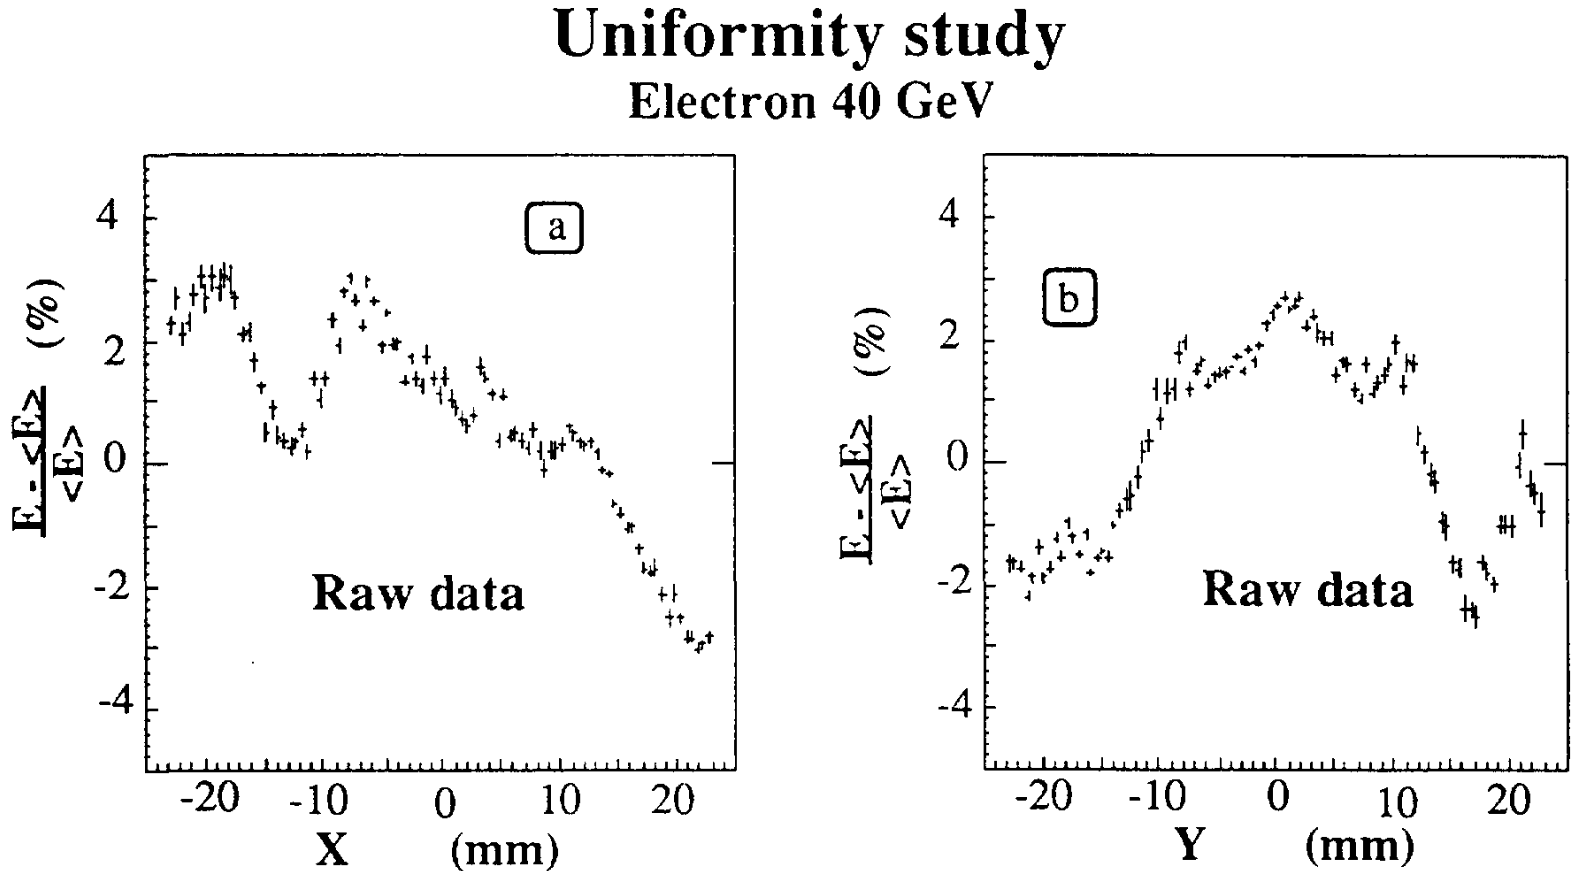
\includegraphics[width=0.48\linewidth]{images//illustrative/shashlyk-resolution-raw.png}
    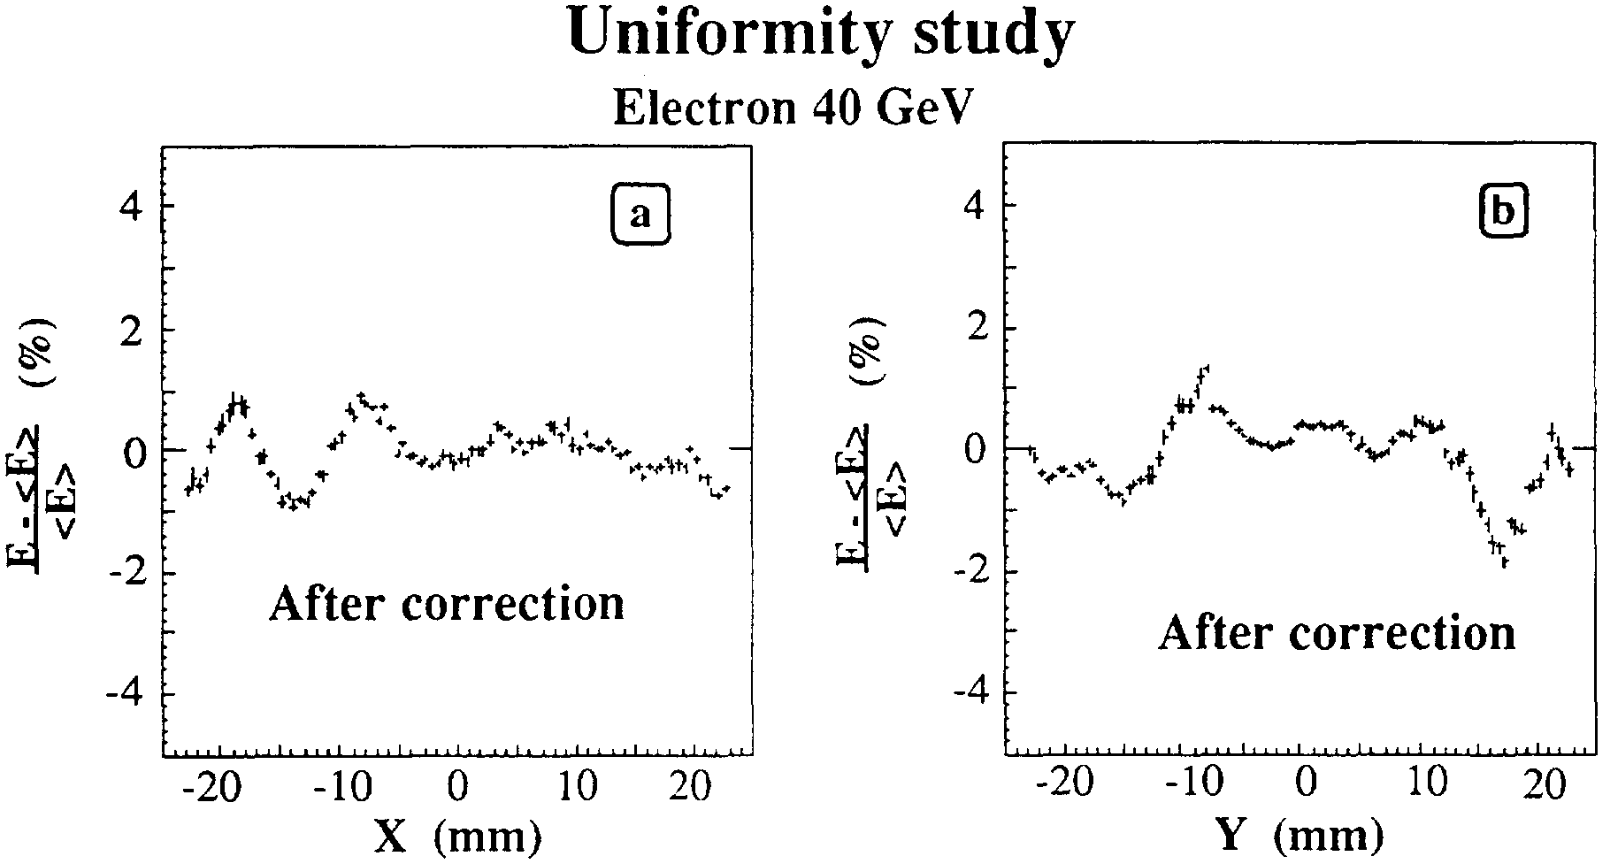
\includegraphics[width=0.48\linewidth]{images//illustrative/shashlyk-resolution-corrected.png}
    \caption{Зависимость оценки энерговыделения калориметра от координаты до и после коррекции согласно работе~\cite{rd36-shashlik-1996}}
    \label{fig:shashlyk-correction-quote}
\end{figure}

Результаты измерения энергетического разрешения
конструктивно-аналогичного калориметра опубликованы
в работе~\cite{chirkovzorin-compass-ecal}. За исключением
фотоприёмника и числа слоёв,
калориметр~COMPASS использует аналогичную NA64 конструкцию
ячеек, включая поперечные размеры, толщины слоёв, марку оптического
волокна и т.д. Полученная зависимость изображена на
рисунке~\ref{fig:chirkovzorin-compass-ecal}.
\begin{figure}
    \centering
    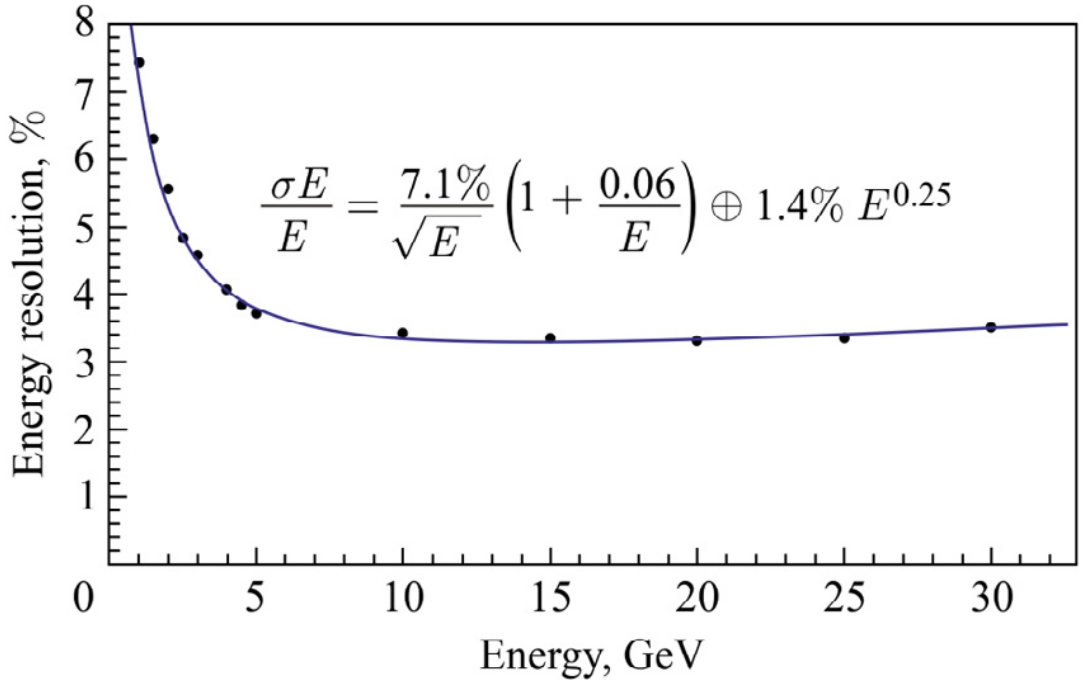
\includegraphics[width=0.5\linewidth]{images//illustrative/compassII-ecal.png}
    \caption{Относительное разрешение ECAL COMPASS фазы II, согласно~\cite{chirkovzorin-compass-ecal}}
    \label{fig:chirkovzorin-compass-ecal}
\end{figure}

Экстраполяция оценки относительного разрешения из этой работы до номинальной
энергии пучка NA64 ($100~\text{ГэВ}$) даёт значение $\simeq 5{,}14~\text{ГэВ}$.
Следует учесть, что практически разрешение должно быть несколько лучше,
поскольку линейный член в работе~\cite{chirkovzorin-compass-ecal}
отвечает за флуктуацию продольных утечек (и обуславливает ухудшение
относительного разрешения на рисунке~\ref{fig:chirkovzorin-compass-ecal}.

%---

%Для апостериорного вычисления коэффициентов
%выражения~\eqref{eq:ecalResolution}, прямая сумма $\oplus$ раскрывается
%следующим образом:
%\begin{equation}
%    \frac{\sigma (E)}{\langle E \rangle} = \sqrt{ \frac{c^2}{\langle E \rangle} + \frac{b^2}{\langle E \rangle^2} + \left( \frac{\sigma(p)}{p} \right)^2 },
%\end{equation}
%где $\sigma(p)/p$ --- импульсное разрешение установки.
% ^^^ проверить, взял https://arxiv.org/abs/hep-ex/0001020 , стр 11, ф-ла (42)

%Текущий раздел будет посвящён отысканию коэффициентов в
%формуле \eqref{eq:ecalResolution} и созданию параметрической модели
%электромагнитного ливня для дальнейших приложений.

\subsection{Адронный калориметр}

В качестве адронного калориметра в NA64 установлен
нескомпенсированный калориметр железо-\acrshort{pmma}.
Калориметр имеет поперечную сегментацию $3\times3$
и состоит из четырёх независимых модулей. В рассматриваемых
в данной работе постановках эти модуле, как правило, ориентируются
вдоль по оси пучка и устанавливаются подряд, совместно с ECAL
образуя герметичный детектор.

Конструктивно, каждый модуль калориметра выполнен в виде
сварной металлической конструкции, в которую помещаются
вкладыши со сборками сцинтилляционных пластин из \acrshort{pmma}
обёрнутых в металлизированный майлар, с выведенными наружу
сцинтилляционными волокнами, как показано на рисунке~\ref{fig:hcal-module}.

Толщина одной $192\times194~\text{мм}$ сцинтилляционной
пластины -- $4~\text{мм}$, поглотителя -- $25~\text{мм}$.
Во вкладыше пластины расположены с небольшим зазором для обеспечения
выхода волокна, так что общая длина одного модуля калориметра
состоящего из 48-и слоёв составляет $1500~\text{мм}$, обеспечивая,
таким образом длину ядерного взаимодействия $7.43 \lambda_I$.

% Плотности:
%   Сталь: 48*25 = 120 см
%   ПММА: 48*4 = 19.2 см
% Длины взаимодействия (PDG):
%   Сталь: \lambda_I = 132.1 г/см^3 => 16.77 см при плотности 7.874 г/см:3
%   ПММА:  = 83.0 г/см:2, плотность 1.16-1.20 г/см^3 => \lambda_I = 70 см
% Число ядерных длин = 120/16.77 + 19.2 / 70.3 = 7.43

\begin{figure}
    \centering
    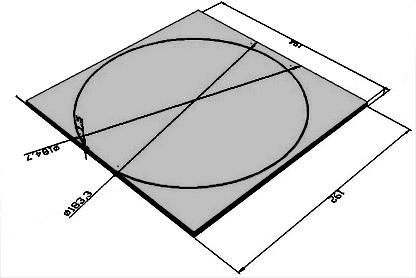
\includegraphics[width=0.3\linewidth]{images/hcal-cell-single-plastic-element.png}
    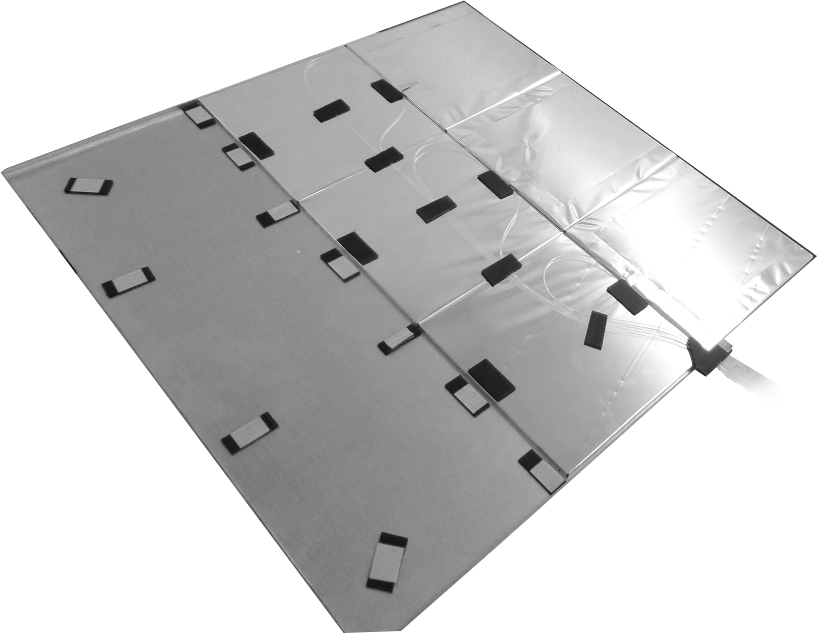
\includegraphics[width=0.3\linewidth]{images//illustrative/hcal-inlet-photo.png}
    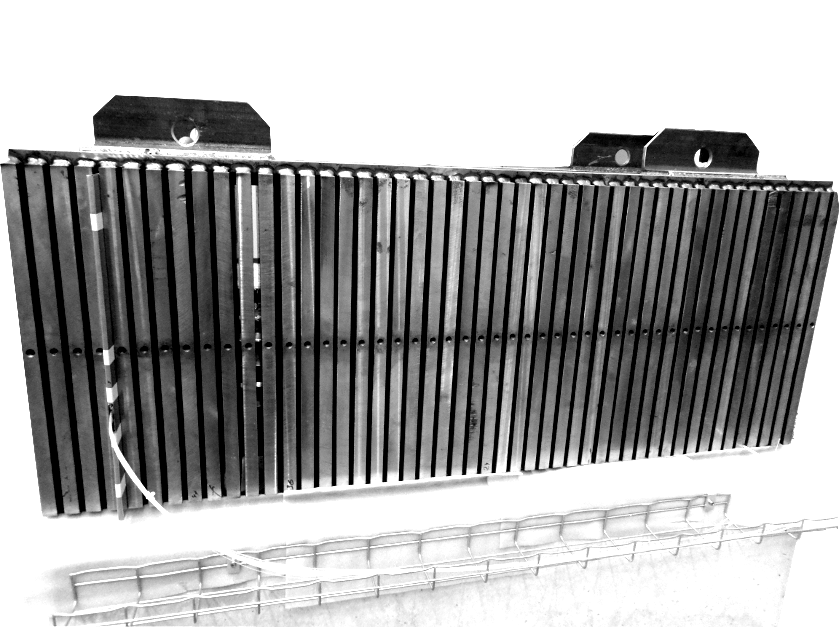
\includegraphics[width=0.3\linewidth]{images//illustrative/hcal-frame-photo.png}
    \caption{Схема укладки оптического волокна, фотографии вкладыша и сварного каркаса HCAL~\cite{PolyakovHCALDrawings-na64site}}
    \label{fig:hcal-module}
\end{figure}

Для задач калибровки калориметра важно, что \acrshort{mip} для
заряженных мюонов $\simeq1{,}55~\text{ГэВ}$ ($32{,}4~\text{МэВ}$ на слой)

Волокна от пластин отвечающих выделенному продольному направлению
соединяются на фотокатоде одного~\acrshort{pmt}, предоставляя
информацию об одной чувствительной пространственной <<ячейке>>
ориентированной вдоль пучка.

Детектор играет важнейшую роль в случаях, когда в электромагнитном
калориметре происходит адронизация компонент
ливня (<<адронный хвост>>) -- в
основном это реакции с выходом пионов: фотоядерные
реакции~$\gamma + Z \rightarrow \pi + Z$ (десятки мб на ядро Pb),
каскадные реакции оброзования т.н. leading
neutrals \cite{leading-neutron-hera} (нейтронов и каонов)
фотодезинтеграция ядер, фоторождение $\eta$-мезонов ($0{,}01$ мб),
адронизация через $\rho$-мезон и т.д. Интегральная вероятность
образования высокоэнергетических нейтральных адронов с энергией
от одного до $100~\text{ГэВ}$ составляет $10^{-9}-10^{-8}$
частиц на инициирующий электрон. Для статистики
свыше~$10^{12}$ играет значительную роль также нейтральная компонента
исходного пучка (т.н. адронное
загрязнение $\pi^0$, $K^0$, $\gamma$-кванты), обсуловленное
методами получения первичного пучка, которые также
идентифицируется HCAL опираясь на пространственные
характеристики ливня.

\subsection{Микроструктурные детекторы}

В качестве трековых детекторов высокого разрешения в NA64 применяются
детекторы GEM (Gas Electron Multiplier)~\cite{gems-sauli} и 
MicroMega (MICRO-MEsh GAseous Structure)~\cite{na64-BANERJEE201872}. Оба типа детекторов
относятся к семейству т.н. \emph{микроструктурных детекторов с газовым
усилением}. Общая идея регистрации заряженной частицы этими детекторами
состоит в регистрации электронной ионизационной лавины развивающийся
в газовой смеси при прохождении заряженной частицы планарной структурой
из тонких (десятки-сотни мкм) электродов.

Основное отличие GEM и MicroMega заключается в конструктивной реализации
принципа газового усиления. В детекторах GEM усиление реализуется за счёт
локального увеличения напряжённости вблизи отверстий перфорирующих тонкую
полимерную фольгу с металлизацией, на которую подаётся разность потенциалов.
Считывание затем производится с металлизированного катодного слоя на
стенке газового объёма, как изображено на рисунке~\ref{fig:gem-charge-collection}.
\begin{figure}
    \centering
    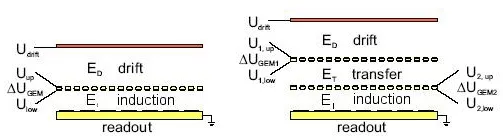
\includegraphics[width=0.65\linewidth]{images//illustrative/gem-charge-collection.png}
    \caption{Схематическое изображение гальванического усиления и зарядового
    считывание в объёме детектора GEM \cite{gems-compass}}
    \label{fig:gem-charge-collection}
\end{figure}
В детекторах MicroMegas, напротив, усиление происходит в узком газовом
зазоре между анодной платой и тонкой металлической сеткой, создающей
градиент электрического поля как показано на рисунке~\ref{fig:mumega-charge-collection}.
Таким образом, в GEM принцип газового
усиления реализуется каскадом электродов, а MicroMegas --
однородной областью лавинного умножения непосредственно над анодом.
\begin{figure}
    \centering
    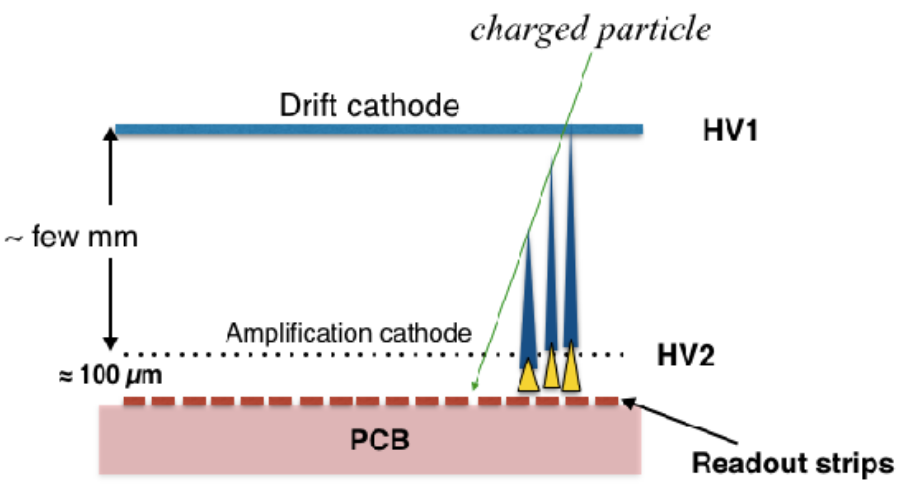
\includegraphics[width=0.65\linewidth]{images//illustrative/mm-charge-collection-example.png}
    \caption{Регистрация треков в рабочем объёме детектора MicroMega \cite{na64-BANERJEE201872}}
    \label{fig:mumega-charge-collection}
\end{figure}

В NA64 оба типа детекторов представлены в микростриповом исполнении --
анод выполнен в виде полос нанесённых литографическим методом на тонкую
подложку (каптон). Каждая такая плоскость даёт информацию
о координате вдоль одного направления. Для восстановления пространственной
точки попадания частицы в рабочий объём плоскости монтируются в виде
отдельных станций состоящих из двух плоскостей, дающих проекционную
информацию о месте развития электронной лавины вдоль пары перпендикулярных
координатных осей (годоскопический принцип).

%TODO: размеры
Рабочий объём детекторов продувается смесью $\text{Ar}/\text{CO}_2$ 80/20\%
при атмосферном давлении.

Считывание электрических сигналов осуществляется посредством
демультиплексирования амплитудных импульсов со всего массива полос на
плоскости и последующего преобразования амплитудного сигнала в цифровую форму.
За аналоговое демультиплексирование отвечает интегральная
микросхема APV~\cite{apv-jones},
в то время как сэмплирующее амплитудно-цифровое преобразование осуществляется
микросхемой MSADC.

Несмотря на хорошее координатное разрешение ($\simeq 300-400\text{мкм}$
при ширине анодной полоски $250~\text{мкм}$ для MicroMegas и $200~\text{мкм}$
при ширине $140~\text{мкм}$ для GEM) и
устойчивость отклика при высоких загрузках, микроструктурные
детекторы NA64 имеют ограниченную площадь чувствительной поверхности
($180\times180~\text{мм}$ для MicroMegas и $102{,}4\times102{,}4~\text{мм}$
для GEM) и применяются в основном в системе мечения.

\subsection{Детекторы на основе тонкостенных трубок}

Для увеличения аксептанса, трекер NA64 может быть оснащён станциями
состоящими из тонкостенных дрейфовых трубок~(\emph{straw})~\cite{straws-volkov2019, straws-peshekhonov2015}.
Каждая трубка представляет собой цилиндрическую поверхность выполненную
из гибкой полимерной плёнки с металлизацией (катода) с протянутой
вдоль её оси проволокой-анодом. Через массив трубок продувается
смесь $\text{Ar}/\text{CO}_2$ (80/20\%) при атмосферном давлении.

Принцип измерения координат основывается на регистрации времени дрейфа
ионизационных электронов к аноду отдельной трубки, как показано
на рисунке~\ref{fig:straws-measurement}.

\begin{figure}
    \centering
    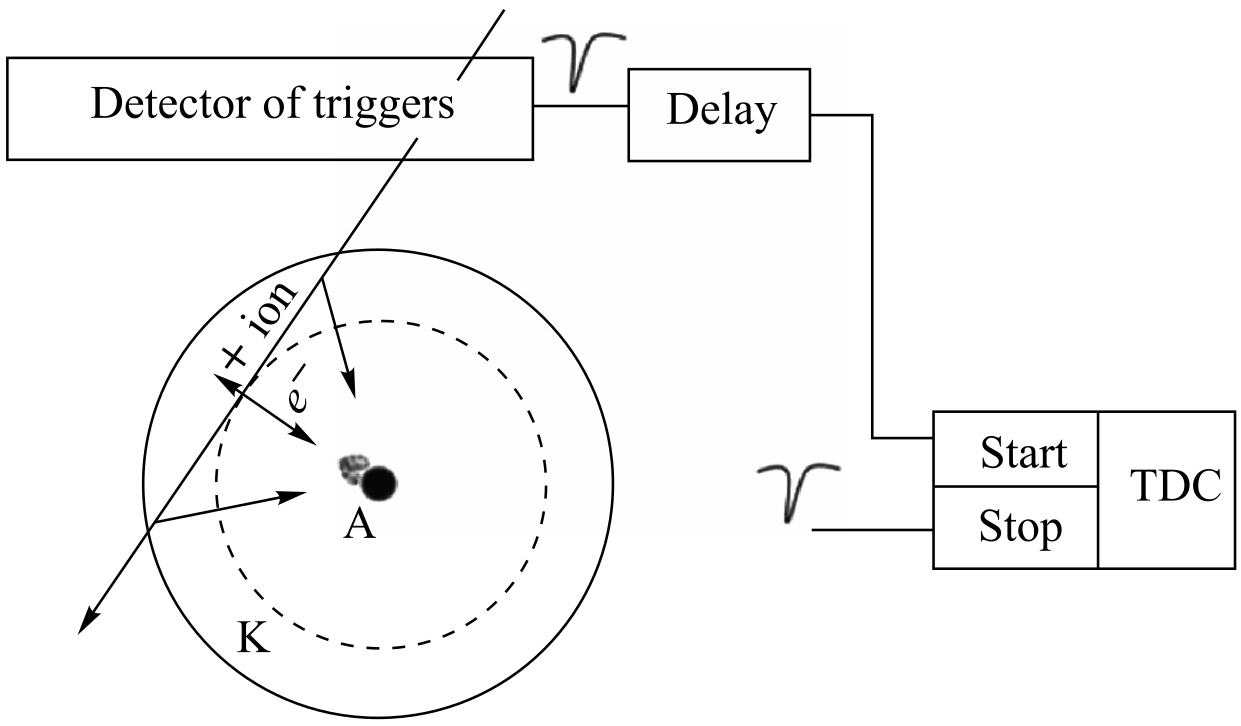
\includegraphics[width=0.5\linewidth]{images//illustrative/strawa-principle.png}
    \caption{Схема измерения времени дрейфа ионизационных электронов~\cite{straws-peshekhonov2015}}
    \label{fig:straws-measurement}
\end{figure}

Для NA64 были изготовлены станции трёх типов:
\begin{itemize}
    \item $200\times200~\text{мм}$ С внутренним диаметром
    трубок $6{,}02 \pm 0{,}025~\text{мм}$, и толщиной
    стенки~$62~\text{мкм}$, с металлизацией алюминием толщиной $500~\mathring{\text{A}}$.
    В качестве анода используется позолоченная вольфрамовая проволока диаметром $30~\text{мкм}$.
    \item $200\times200~\text{мм}$ С внутренним диаметром
    трубок $2 \pm 0{,}025~\text{мм}$, и толщиной
    стенки~$67~\text{мкм}$, с металлизацией алюминием толщиной $200~\text{нм}$
    и дополнительным покрытием защитным слоем графитополиуретана толщиной~$6~\text{мкм}$.
    В качестве анода используется позолоченная вольфрамовая проволока диаметром
    $20~\text{мкм}$.
\end{itemize}

С точки зрения трекинга, измеренное время сигнала $t$ с анода задаёт
изохронную цилиндрическую поверхность с радиусом $r = t v$, где
$v$ -- характерная скорость дрейфа электронов в газовой смеси.
Алгоритмически, такие изохронные поверхности способны приводить к
неоднозначностям при реконструкции трека, поэтому станции обычно состоят
из массивов тонкостенных дрейфовых трубок или являются частью
многоступенчатого трекера.

\subsection{Номенклатура детекторов}

С целью охвата всей номенклатуры детекторов в рамках программных
моделей имеющих дело с данными эксперимента в общем (и с моделью
события в частности), необходимо учесть следующие обстоятельства,
связанные с представлением данных на низком уровне 

На уровне отдельных измерений, состав (тип и топология)
данных полностью определяется основной микросхемой (\emph{чипом})
считывающего электронного устройства, осуществляющего
преобразование аналоговых сигналов.
Это означает, в частности, что сигналы оцифрованные с калориметра,
пучкового счётчика, вето-детектора и мюонного счётчика будут
содержать одну и ту же информацию в смысле типа данных, поскольку
считываются одним и тем же чипом. В то же
время, сигнал от микроструктурных детекторов --- будь
то GEM или MicroMega будут иметь другой тип данных.

Таким образом, с точки зрения физического представления данных,
целесообразно поместить показания от одного чипа в
гомогенную коллекцию. Тогда статический
\gls{allocator} коллекции будет иметь дело
с данными одного типа, что уменьшит фрагментацию данных и
улучшит локальность кэширования. Дополнительным преимуществом
такого решения является возможность итерировать всю такую коллекцию
в рамках одной лексемы -- во многих случаях прикладные алгоритмы
(обработчики конвейера данных) нуждаются в доступе такого вида.
Например, алгоритм вычисления сигнала нулевого уровня
совершенно агностичен к тому, к какой станции,
или к какому типу детекторов относится оцифрованный сигнал.

Следующим важным элементом классификации детекторов является деление
по \emph{семействам} (англ. \emph{kin}), для которых в системе
сбора данных NA64 приняты обозначения подобные приведенным в
таблице \ref{tab:detector-names-examples}.

\begin{table}[ht]
\centering
\begin{tabular}{r|cl}
Наименование & Чип     & Описание \\ \hline
          S1 & MSADC   & Первый пучковый счётчик \\
        VETO & MSADC   & Вето-детектор \\
        ECAL & MSADC   & Электромагнитный калориметр \\
        GM03 & APV     & Газовый электронный умножитель №3 \\
        MM02 & APV     & Микросеточный газовый детектор №2  \\
        ST06 & NA64TDC & Трубчатый дрейфовый детектор №6
\end{tabular}
\caption{Примеры имён детекторов}
\label{tab:detector-names-examples}
\end{table}

Наконец, необходимо индексировать отдельные чувствительные
элементы детектора. В зависимости от семейства к которому принадлежит
детектор, это могут быть ячейки калориметра, проекционные
плоскости трековых детекторов, трубки газовых детекторов.

В результате, дескриптор уникально идентифицирующий чувствительный
элемент детектора должен отражать следующую семантику (в порядке
убывания общности):

\begin{enumerate}
    \item Идентификатор типа микросхемы (чипа, <<chip>>), определяющий
    тип данных,
    \item Идентификатор семейства детектора (<<kin>>), дающий информацию о
    физическом смысле сигнала,
    \item Номер станции, для уникальной идентификации детектора в
    пределах одного семейства,
    \item Нагрузку (<<payload>>), содержащую информацию о конкретном
    чувствительном элементе детектора, в зависимости от чипа или семейства.
\end{enumerate}

Для калориметров и сегментированных детекторов с \acrshort{pmt},
нагрузке достаточно содержать три индекса, идентифицируюших
ячейку или сегмент детектора.

Для микроструктурных трековых детекторов нагрузка должна содержать
информацию об ориентации проекционной плоскости детектора и номер
чувствительного элемента.

Простой расчёт показывает, что всю номенклатуру детекторов NA64
можно уместить в множестве мощностью не более $2^{64}$ значений,
что позволяет, в принципе, использовать номерной идентификатор
для кодирования дескриптора детектора. Это в свою очередь позволяет свести
операции запроса и поиска элементов коллекций до простых
операций с целым числом фиксированной длины, осуществлять выборку
элементов применением быстрых побитовых операций и т.д.


\begin{comment}
\subsection{Моделирование э/м ливня}

Для оценки вклада в разрешения факторов обусловленных физикой ливня
воспользуемся эмпирической формулой разрешения для слоистого калориметра с
заданной геометрией~\cite{delPeso1989-sampling-calorimeters}:
\begin{equation}
    \frac{\sigma_{sampl}}{E}(\%) = \frac{3.5}{\sqrt{E}}
        \cdot \left( \frac{t}{X_t} \right)^{\alpha}
        \cdot \left( \frac{s}{X_s} \right)^{\beta},
\end{equation}
где $t, X_t, s X_s$ --- толщина и радиационная длина слоёв сцинтиллятора и
свинца, соответственно, а $\alpha, \beta$ --- некоторые подстроечные  % e.g. alpha=0.67, beta=-0.3
коэффициенты, которые обычно определяются из МК-модели
калориметра (в оригинальной работе~\cite{delPeso1989-sampling-calorimeters}
моделирование производилось в пакете EGS4, 1988). % TODO использующего модели
Современный (напр. 4.10.6) Geant4 предоставляет возможность использовать
различные комбинации моделей процессов электромагнитного ливня с тем чтобы
обеспечить наилучшее согласие в известном диапазоне энергий.

Для моделирования развития ливня зададим геометрию калориметра в виде цилиндра
составленного из круговых пластин сцинтиллятора и свинца с толщинами
соответствующих слоёв ECAL. Получившуюся модель цилиндрического калориметра
сегментируем по $\rho, \phi, z$ с тем чтобы для заданной энергии инициирующей
частицы получить \emph{энергетический профиль} э/м ливня в виде функции со
следующей факторизацией:

\begin{equation}
    \dd E(\rho, z) = E/2\pi \cdot f(\rho) \dd \rho \cdot f(z) \dd z.
    \label{eq:emshowerFac}
\end{equation}

Нужно заметить, что факторизация \eqref{eq:emshowerFac} справедлива только для
перпендикулярного направления движения частицы по отношению к пластинам
калориметра. В силу анизотропии размещения поглотителя в веществе калориметра,
такая факторизация перестаёт работать.
% ^^^ интересным приложением может быть реконструкция угла падения частицы на
% основе такой информации --- хотя вклад от \phi по-видимому нельзя
% факторизовать, вероятно возможно подобрать декомпозицию другого рода...

\subsection{Продольный профиль э/м ливня}

Известно, что продольный профиль ливня хорошо описывается
$\Gamma$-распределением \cite{Longo1975EMCSim}:

\begin{equation}
    \left\langle \frac{1}{E} \frac{\dd E(z)}{\dd z} \right\rangle = f(z) = \frac{(\beta z)^{\alpha-1} \beta \exp(-\beta t)}{\Gamma (\alpha)},
\end{equation}
где $\alpha$ регулирует форму продольного профиля а $\beta$ --- масштаб.  %< TODO: "масштаб"?
Центр масс $\langle z \rangle$ энергетического распределения связан с этими
параметрами как $\langle z \rangle = \alpha / \beta$, а максимум может быть
выражен как $\max f(z) = (\alpha - 1)/\beta$.
\end{comment}
\section{Аналого-цифровые преобразователи}

%В NA64 для оцифровки сигнала с \acrshort{pmt} счётчиков, вето-детекторов и
%калориметров применяются аналого-цифровые преобразователи MSADC \cite{MSADC-Mann1, %MSADC-Mann2} (\emph{англ} Mezzanine sampling analog to digital converted).
Для оцифровки сигналов формируемых \acrshort{pmt} (пучковых счётчиков,
вето-детекторов и калориметров) в NA64 применяются
аналого-цифровые преобразователи MSADC \cite{MSADC-Mann1, MSADC-Mann2}
(англ. \emph{Mezzanine Sampling Analog-to-Digital Converter}).
MSADC представляет собой устройство на основе микросхемы
ADS527x~\cite{ADS527x}, выполненное в виде мезонинной карты расширения
в стандарте <<Advanced Telecom Computing Architecture>> (ATCA).
Конструктивно, предусмотрен монтаж устройства как в
корзину (крейт) системы сбора данных, так и в непосредственной близи
детекторной сборки для уменьшения длин аналоговых линий и уменьшения помех.
MSADC в установке NA64 применяются как для непосредственного считывания
сигналов \acrshort{pmt}, так и опосредованно, для оцифровки сигналов
от микропаттерных детекторов предварительно подаваемых на вход
аналогового демультиплексора.

В рамках первого сценария каждый аналоговый канал считывается двумя сэмплирующими
АЦП, работающими на частоте $40\text{МГц}$. Каналы тактируются со
смещением в половину
фазы, обеспечивая сэмплирование сигнала с интервалом 12.5нс (с
частотой~$80\text{МГц}$). На рисунке \ref{fig:msadc-example} приведён
характерный пример гистограммы полученной на основе $8\times10^3$ событий в
центральной ячейке калориметра ECAL, с отбором по пучковому триггеру.

\begin{figure}
    \centering
    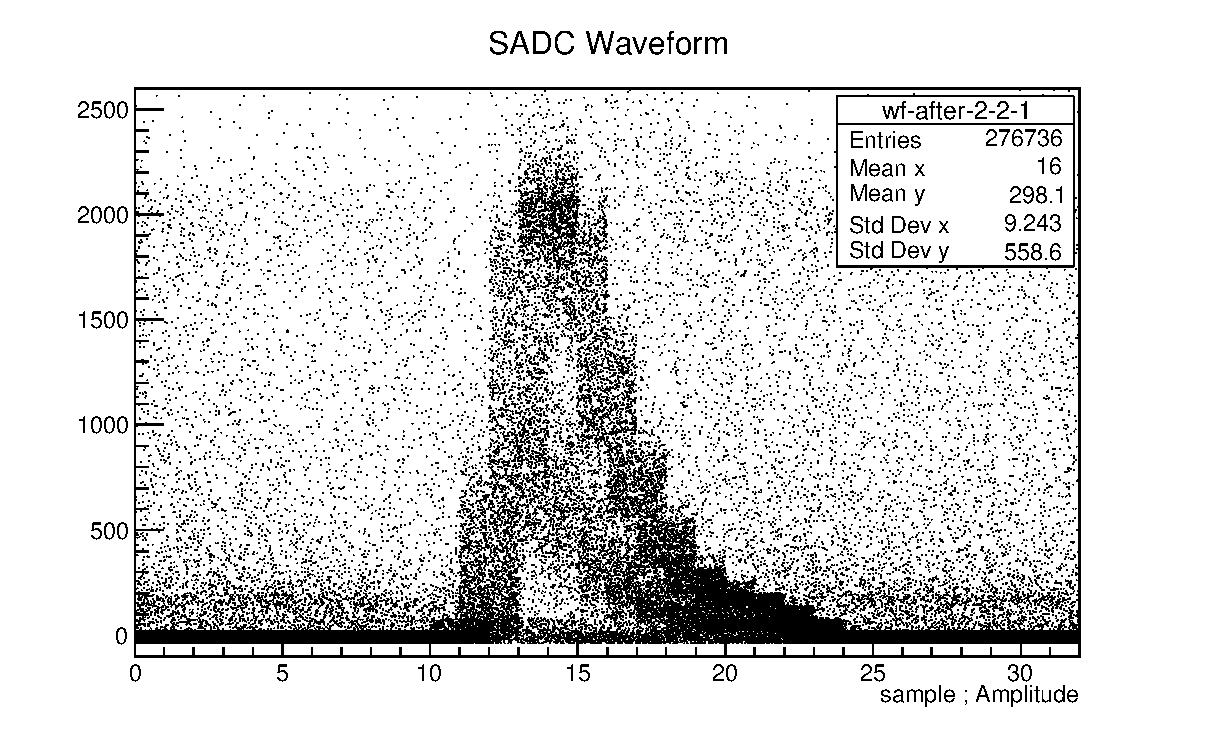
\includegraphics[width=0.65\linewidth]{images/illustrative/msadc-waveforms-example.eps}
    \caption{Гистограмма характеризующая временную развёртку амплитудного сигнала в
    центральной ячейке от моноэнергетического пучка}
    \label{fig:msadc-example}
\end{figure}

Для регистрации сигнала от сцинтилляционных детекторов в эксперименте
применяются ФЭУ-84~\cite{soviet_pmts}, для которых время нарастания
импульса анодного тока не превышает одной наносекунды. При этом
характерная длительность (ширина на половине амплитуды) импульсов от
большинства детекторов лежит в диапазоне от двух до трёх наносекунд.

Следует отметить, что согласно теореме Котельникова (Найквиста-Шеннона),
для безошибочного восстановления сигнала с таким характерным временем,
необходима частота дискретизации не менее $800\text{МГц}$ (частота
Найквиста для сигналов длительностью $2{,}4\text{нс}$).

С целью разрешения единичных импульсов от ФЭУ-84 в основном применяемых в
эксперименте, сигнал от \acrshort{pmt} передаётся сначала на вход
предварительного преобразователя (шейпера выполненого на основе
операционного усилителя AD8021~\cite{ad8021}), увеличивающего характерную
ширину сигнала примерно в три раза с сохранением амплитудной
пропорциональности. Несмотря
на то что частоты $80\text{МГц}$ всё ещё недостаточно для безошибочного
разрешения сигналов с полушириной в диапазоне от $6$ до $9~\text{нс}$
(частота Найквиста составляет примерно $170\text{МГц}$), необходимой
точности восстановления временных характеристик сигналов можно
добиться используя априорную информацию о форме сигнала -- то есть,
подобрав аналитическую модель достаточно хорошо воспроизводящую сигнал,
способную восполнить недостающую информацию в частотном домене.

\subsection{Параметризация сигнала АЦП}

С целью определения основных свойств сигнала и выбора оптимальных моделей для
математической подгонки (фита), для различных детекторов была выполнена серия
измерений формы импульса до и после шейпера с применением цифрового
осциллографа с пикосекундным разрешением.

%При рассмотрении малых амплитуд (менее $100~\text{мВ}$) определённую
%практическую трудность создают различные помехи, обусловленные индуктивными
%эффектами при работе на высоких частотах, такие как эффекты индуктивных
%задержек и отражений в коаксиальных проводниках, неидельность волнового
%сопротивления во цепи между шейпером и осциллографом или \acrshort{pmt} или
%осциллографом. С целью снижения этих эффектов при проверке модели
%параметризации, для проверки модели параметризации в области малых
%амплитуд, было выполнено численное моделирование шейпера на основе его
%принципиальной схемы.
Анализ сигналов малой амплитуды (менее $100~\text{мВ}$) имеет
определённые практические трудности, обусловленные влиянием помех,
связанных с индуктивными эффектами, проявляющимися при работе на высоких
частотах. К числу таких эффектов относятся индуктивные задержки и
отражения в коаксиальных линиях передачи, а также отклонения
волнового сопротивления от номинального в линии связи между
шейпером и осциллографом и между шейпером и \acrshort{pmt}.

Для уменьшения влияния указанных факторов при проверке работоспособности
модели параметризации в области малых амплитуд было выполнено численное
моделирование работы шейпера на основе его принципиальной электрической
схемы в программном пакете LTspice~\cite{ltspice}.

%На рисунке~\ref{fig:ltspice-shaper-simulation} показан пример временной
%развёртки сигнала. Импульсам с отрицательной амплитудой соответствуют
%запись входного сигнала выполненного осциллографом с интервалом
%200 пикосекунд. Импульс с положительной амплитудой отображает результат
%симуляции.

На рисунке~\ref{fig:ltspice-shaper-simulation} приведён пример временной
развёртки сигнала. Импульсы с отрицательной амплитудой соответствуют
результатам регистрации входного сигнала осциллографом с временным шагом
дискретизации 2~пс, тогда как импульс с положительной амплитудой
представляет собой результат компьютерного моделирования.

\begin{figure}
    \centering
    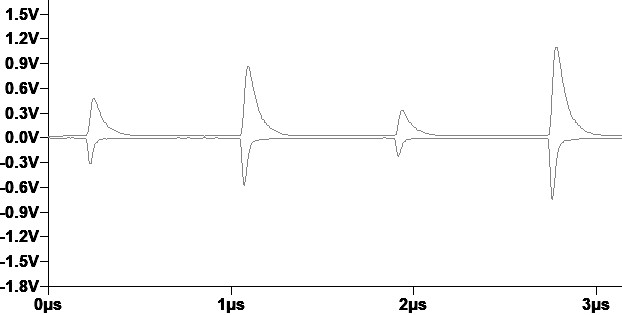
\includegraphics[width=0.75\linewidth]{images//illustrative/shaper-simulation.png}
    \caption{Результат моделирования преобразования сигнала в LTspice}
    \label{fig:ltspice-shaper-simulation}
\end{figure}

Моделирование достаточно хорошо (в пределах 1\%) согласуется с измеренным
выходным сигналом с амплитудами не менее нескольких десятков мВ.
На основании записанного сигнала в области больших
амплитуд, и с использованием численной модели LTspice, производилась проверка многопараметрических аналитических функций, способных воспроизводить форму
сигнала до или после шейпера.

%Количественные критерий, в виду сложной зависимости функции отклика от
%парамтров измерения, были сформулированы на основе важнейших физических
%параметров, а не общего численного соответствия. В частности, не
%рассматривалась точность поведения экспоненциального спадания импульса
%на интервалах превышающих ширину на полувысоте более чем вдвое, поскольку,
%в силу схемотехнических причин, последняя на этом участке слишком сильно
%зависит от парамтров шейпера имеющих большой разброс. Напротив, важными
%параметрами являлись:
Количественные критерии, учитывая сложную зависимость функции отклика
от параметров измерений, были определены на основе ключевых физических
характеристик, и в меньшей степени -- на основе общего численного
совпадения формы сигнала.
При этом не рассматривалась точность аппроксимации экспоненциального
спада импульса на временных интервалах, превышающих удвоенную ширину
на полувысоте, поскольку в данной области форма импульса существенно
зависит от параметров шейпера, характеризующихся значительным
технологическим разбросом.

В качестве основных критериев были выбраны:
\begin{itemize}
    \item Точка на переднем фронте импульса, соответствующая полувысоте
    импульса, принятая в качестве инвариантной временной метки (постоянная
    доля, англ. \emph{constant fraction}),
    \item Амплитуда в абсолютном максимуме импульса, как величина
    пропорциональная энерговыделению.
\end{itemize}

Помимо количественного соответствия сигналам, функции должны достаточно
просты для численного счёта, чтобы их можно было применять в различных
схемах нелинейной минимизации, таких как метод Ньютона, метод градиентного спуска
или алгоритм Левенберга-Марквардта~\cite{marquardt-lms}.

Итак, согласно выбранным критериям, рассматриваются следующие функции:

\begin{itemize}
    \item Функция Мояла \cite{moyalFunction} с тремя параметрами, определяемая выражением
    \begin{equation}
        F_M(t) = \frac{A}{\sqrt{2 \pi}} \exp \left\{ - \frac{1}{2} \left(\frac{x - \mu}{\sigma}+ \exp\left(\frac{x - \mu}{\sigma}\right)\right) \right\}
        \label{eq:moyalFNormed}
    \end{equation}
    которая адекватно описывает результат преобразования сигнала
    шейпером, позволяя использовать сравнительно простые аналитические формулы
    для временных характеристик (например, точки перегиба на переднем фронте) и амплитуды. Несмотря на присутствие быстро растущего множителя
    $e^{e^x}$, функция демонстрирует численную устойчивость при минимизации методом Левенберга–Марквардта с ускорением сходимости градиентом.
    \item Функция специального вида (N-pole), появляющаяся при различных
    аппроксимациях в некоторых статистических приложениях гамма-функции~\cite{gamma-stegun}:
    \begin{equation}
        f_{Np}\left(x\right)=A\left(x-t_{0}\right)^{n}e^{-\frac{\left(x-t_{0}\right)}{T}}\ \left\{x>t_{0}\right\}
    \end{equation}
    %хорошо описывает форму импульса до шейпера, воспроизводя быстрый рост
    %переднего фронта и обеспечивая устойчивые оценки
    %временных характеристик. При этом, аналитические выражения для времени
    %и амплитуды сигнала требуют вычисления специальных функций (гамма функции
    %и $W$ Ламберта). Из-за быстрого роста параметра $n$ функция требует
    %применения масштабных преобразований, иначе её сходимость нестабильна.
    %Также, при разрешении вкладов от близких по времени импульсов, функция
    %требует введения апостериорных ограничений для разрегения неоднозначности.
    которая хорошо воспроизводит форму импульса до шейпера, обеспечивая
    быстрое нарастание переднего фронта и стабильные оценки временных
    параметров. При этом аналитические выражения для времени и амплитуды
    сигнала требуют вычисления специальных функций --- гамма-функции и
    $W$-функции Ламберта. Из-за быстрого роста параметра $n$ функция
    требует применения масштабных преобразований для обеспечения
    сходимости численных алгоритмов. Кроме того, при разрешении
    наложенных импульсов с близкими по времени появлениями требуется
    введение апостериорных ограничений с целью устранения
    неоднозначностей.
    \item Четырёхпараметрическая функция из работы \cite{optimal-pulse-proc-samoyl}:
    \begin{equation}
        F(t) = A \cdot \exp(-(t-t_0)/\tau_1) /(1 + \exp(-(t-t_0)/\tau_2).
    \end{equation}
    %используется для аппроксимации импульсов с малой амплитудой. Практически,
    %независимость левого и правого фронтов приводят к необходимости
    %введения ограничений на основе апостериорных оценок.
    позволяющая независимо описывать участки нарастания и спада
    импульса. Эта функция применяется для аппроксимации сигналов
    малой амплитуды. Практически независимость параметров левого и
    правого фронтов требует введения апостериорных ограничений для
    обеспечения устойчивости.
\end{itemize}

%Применение описанных моделей позволяет описывать сигналы \acrshort{pmt}
%сэмплирующих АЦП в широком диапазоне энергий. В силу
%нелиности процедуры минимизации, наличия локальных
%минимумов, аппаратных шумов, а так же неоднозначности при разрешении
%вкладов от нескольких близких по времени частиц, практическое
%использование описанных параметризаций должно производиться в рамках
%программного окружения допускающего конкурентные сценарии,
%резервные алгоритмы условные ветвления и итеративную проверку гипотез.
Применение рассмотренных моделей позволяет адекватно описывать сигналы
\acrshort{pmt}, считываемые сэмплирующими АЦП в широком диапазоне энергий.
Ввиду нелинейности процедуры минимизации, наличия локальных минимумов
функции ошибки, а также влияния аппаратных шумов и неоднозначности при
разложении сигналов, формируемых несколькими близкорасположенными
во времени частицами, практическое использование данных параметризаций
должно осуществляться в программном обеспечении, обеспечивающем
поддержку конкурентных сценариев, резервных алгоритмов, условных
ветвлений и итеративной проверки гипотез.

\subsection{Уровень нулевого сигнала и эффекты высокой частоты}

%Уровнем нулевого сигнала (\emph{baseline}) называется значение оцифрованной
%амплитуды соответствующее отсутствию физического сигнала. Это значение
%обусловлено входным напряжением операционного усилителя во входном каскаде АЦП и
%балансировкой внутренних компараторов. Также, это значение определяется
%внутренними параметрами цепи и может быть подвержено
%незначительному дрейфу~($<1\%$), обусловленному изменениями гальванических
%характеристик линий преобразователя или изменением темнового тока \acrshort{pmt}
%под воздействием высокой интенсивности, термическими
%эффектами схемы, статистическими флуктуациями электронной лавины.
\emph{Уровнем нулевого сигнала} (\emph{baseline}) представляет собой значение оцифрованной амплитуды, соответствующее отсутствию сигнала на входе АЦП.
Формирование данного уровня обусловлено входным напряжением операционного
усилителя, используемого во входном каскаде АЦП, а также балансировкой
внутренних компараторов. Помимо этого, значение нулевого уровня определяется
внутренними параметрами входной цепи и может подвергаться незначительному
дрейфу (порядка $1 \%$ от уровня сигнала, что способно оказать заметное
влияние на разрешение некоторых детекторов), вызванному изменением
гальванических характеристик линий преобразователя, вариациями темнового
тока \acrshort{pmt} под воздействием высокой интенсивности, термическими эффектами
в электронной схеме, а также статистическими флуктуациями электронной
лавины.

Для повышения точности реконструкции энерговыделения в калориметре
необходимо применять устойчивый алгоритм выделения нулевого уровня, который бы
в наименьшей мере подвержен влиянию дрейфа и эффектам связанным с
интенсивностью пучка.

Существующий алгоритм динамического вычисления нулевого уровня заключается
в анализе первых нескольких сэмплов амплитудного сигнала и опирается на
предположение о том что в них отсутствует фактический сигнал. Последнее
обстоятельство гарантируется триггерной системой в смысле сигналов от
первичных частиц отслеживаемых триггерными счётчиками. Практически, нередки
события, когда сигнал в детекторе присутствует и обусловлен гало пучка, 
вторичными частицами и т.д. Если разброс
минимального и максимального значений превышает некоторый заданный порог,
за уровень нулевого сигнала берётся минимальное значение, в противном случае,
вычисляются средние. Результат работы такого алгоритма определяется
абсолютным порогом. На рисунке~\ref{fig:baselineresults} слева изображён
вариант работы такого алгоритма в случае, когда в окне оцифровки присутствует
остаточный сигнал от предыдущего события с амплитудой не превышающий
порог. Для наглядности, справа приведён результат работы улучшенного
алгоритма предложенного автором на основе минимизации невязок вторых
производных (\emph{деинтерлейсинг}), вместе с изображением результатов
аппроксимации модельными функциями.

\begin{figure}
    \centering
    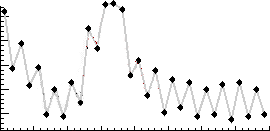
\includegraphics[width=0.33\linewidth]{images//illustrative/baselines-distorted.png}
    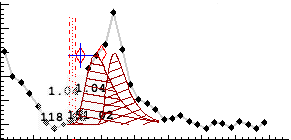
\includegraphics[width=0.33\linewidth]{images//illustrative/baselines-corrected.png}
    \caption{Отыскание нулевого уровня сигнала
    по первым сэмплам (слева) и на основе минимизации производных (справа)
    в относительных единицах}
    \label{fig:baselineresults}
\end{figure}

%В качестве иллюстрации, рассмотрим сигналы изображённые на рисунке ...

Появление отдельных событий на триггере установки определяется средней
интенсивностью пучка, и их число в любой конечный интервал времени является
случайной величиной, распределение которой соответствует закону
Пуассона~\cite{exp-methods-Abramov1977}.
Управляемая средняя частота триггерных событий
обычно выбирается таким образом чтобы влияние событий оказавшихся в пределах
одного временного окна считывания данных было не слишком велико (обычно
от 5 до 40\% в окне $400~\text{нс}$).

Идентификация таких событий имеет важное значение в первую очередь на этапе
калибровки, поскольку будет обуславливать систематическую ошибку средних
величин для заранее неизвестного энергетического вклада.

\iffalse
Руководствуясь первыми принципами возможно оценить статистический вклад от
таких событий с тем чтобы рассчитать соответствующие поправки, если известна
функция отклика от незашумлённых данных.

%Рассмотрим например детекторы, считывание данных с которых производится чипом
%MSADC (сэмплирующий АЦП) --- чип оцифровывает гальванический сигнал (обычно
%амплитудный испульс с \acrshort{pmt} после шейпера) в виде набора отдельных измерений с
%фиксированным интервалоом в пределах короткого временного окна. В качестве
%модельного приближения выберем далее функцию Мояла \cite{moyalFunction}:

%в которой, помимо положения максимума $\mu$ введём дополнительные параметры
%отвечающие за ширину и площадь ($\sigma$ и $S$):
%\begin{equation}
%    M(t, \vec{p}) = \frac{S}{\sqrt{2 \pi} \sigma} \exp\left\{ - \frac{1}{2} \left(\frac{t-\mu}{\sigma} + \exp\left(-\frac{t-\mu}{\sigma}\right)\right) \right\}.
%\label{eq:moyalF}
%\end{equation}

%Функцию \eqref{eq:moyalFNormed} обычно используют в качестве аналитической
%аппроксимации функции плотности распределения Ландау \cite{BockHEPFormulae}.

Задержка сигнальной линии относительно триггера выбирается таким
образом, чтобы разместить максимум импульса в середине сэмплирующего окна,
а для вычисления пьедесталов производится по первым нескольким каналам таким
образом, чтобы им соответствовал вероятный ноль сигнала.

\begin{figure}[h]
    \centering
    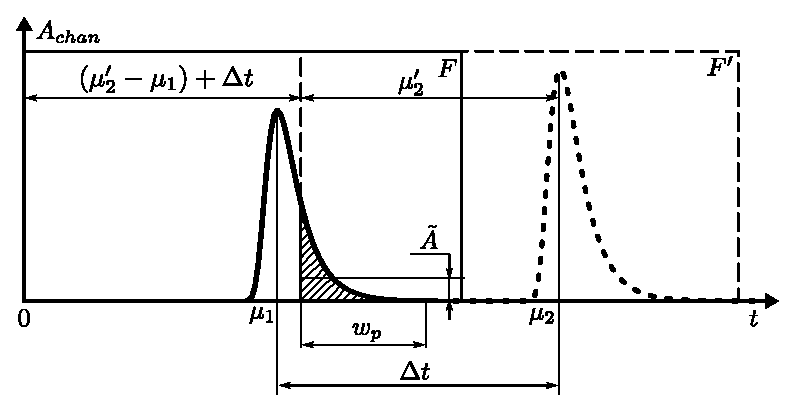
\includegraphics[scale=1.05]{pile-up-image-v2.eps}
    \caption{Схематическое изображение эффекта pile-up в амплитудно-временной
развёртке \acrshort{pmt}. Здесь, при оцифровке триггерного события (показано
пунктиром, вместе со своим окном дискретизации~$F'$) с максимальной
амплитудой в момент времени~$\mu_2 = \Delta t + \mu_2'$, в качестве значения
пьедестала будет взято среднее значение~$\tilde{A}$ на участке~$w_p$ которое
оказывается смещено относительно настоящего нуля за счёт вклада от события
$\mu_{1}$ (показано непрерывной линией вместе со своим окном дискретизации~$F$).}
    \label{fig:pileUpDiagram}
\end{figure}

Значение пьедестала $\tilde{A}$ определённое в окне
$w_p$, для каких-нибудь двух событий отклики которых заданы двумя наборами
параметров
$\mu_1, \sigma_1, S_1$ и $\mu_2, \sigma_2, S_2$, и произошедших с интервалом
$\Delta t$ можно записать в виде математического усреднения (см.
рис. \ref{fig:pileUpDiagram}):

\begin{equation}
\tilde{A} = \frac{1}{w_p} \int\limits_{\Delta t}^{\Delta t + w_p} (M(t, \mu_1, \sigma_1, S_1) + M(t, \mu_2, \sigma_2, S_2) \dd t
\end{equation}

Вклад $M(t, \mu_2, \sigma_2, S_2)$ будет ничтожным поскольку $w_p$ выбирается таким
образом, чтобы перекрыть участок до переднего фронта импульса триггерного
события, а дисперсия $\mu$ незначительна относительно ширины окна дискретизации
и $w_p$. Таким образом, модель можно редуцировать до плавающего окна усреднения
единственной функции $M(t, \mu_1, \sigma_1, S_1)$. Опустим индексы
для краткости, поскольку параметры триггерного события не влияют на результат: 

\begin{equation}
    \tilde{A}(\Delta t, \mu, \sigma, S) = \frac{1}{w_p} \int\limits_{0}^{w_p} M(t, \mu - \Delta t, \sigma, S) \dd t.
    \label{eq:avPedestal}
\end{equation}

Практический интерес представляет зависимость средней ошибки пьедестала от
средней частоты событий --- решение такой задачи даёт критерий для контроля
качества данных. Для того чтобы получить такую оценку аналитически, можно,
далее, взвесить и усреднить
функционал \eqref{eq:avPedestal} по $\Delta t$ и набору параметров
$\mu, \sigma, S$.


При этом, для правдоподобия модели критическое значение имеет
скоррелированность параметров $p_{n,(1)}$, --- в таком распределении
заключена основная информация о характере функции отклика единичного события.
Общий вид трёхмерной гистограммы распределения этих параметров показан на
рис. ???.
%TODO: 3D-гистограмма

Если каким-нибудь образом гарантировать отсутствие pile-up-событий в
гистограмме на рис. ???, то получившимся распределением можно воспользоваться
в качестве параметризации параметра модели.

Для частоты событий $\nu$ интервал между случайными событиями $\Delta t$
подчиняется экспоненциальному закону, таким образом среднее значение
пьедестала:

\begin{equation}
    \bar{A} (\nu) = \frac{\nu}{w_p} \int\limits_0^{\infty} \exp(- \Delta t \nu ) \left(
        \int\limits_{0}^{w_p} M(t, \mu - \Delta t, \sigma, S) \dd t \right) \dd \Delta t
\end{equation}
\fi

\section{Анализ данных}

Весьма важен вопрос анализа данных,
как процедуры обработки экспериментальных данных
направленной на проверку определённых статистических гипотез.
%В самом деле, процедуры сложно разделить
%практически, поскольку алгоритмы реконструкции содержат
%различные подстроечные параметры выбираемые из статистических
%соображений, с учётом физического процесса лежащего в основе
%конкретного измерительного процесса.

Сложившаяся практика работы с экспериментальными
данными обычно подразумевает разделение фаз отладки процедур
физической реконструкции событий и физического анализа данных.
У этого разделения есть как технические, так и методические причины.

К техническим относятся, например, многоэтапность процедуры
реконструкции, часто включающая применение итеративных операций,
использование алгоритмов с обратной связью. Кроме того,
%как уже отмечалось,
реконструкция в современном физическом эксперименте
как правило, представляет собой чрезвычайно требовательную задачу
к вычислительным ресурсам. По этой причине результат
реконструкции обычно сохраняется в виде промежуточных данных,
удобных для последующего анализа.

К методическим относится, например,
стратегии <<слепого анализа>>~\cite{blind-analysis} (анализа по слепому методу)
предписывающая экспериментатору исключать из рассмотрения
параметрические области, в которых может присутствовать исследуемый
сигнал до тех пор, пока все алгоритмы реконструкции и критерии отбора,
а также все процедуры анализа не окажутся
зафиксированы, и все проверки независимых данных, систематических
ошибок и методы статистической интерпретации результата не будут
выполнены.

Поскольку NA64 направлен прежде всего на поиск гипотетических частиц,
основная задача анализа сводится в вероятностном
смысле к проверке гипотезы $H_0$ о средней частоте событий с
заданным уровнем \emph{статистической значимости}~$\alpha$
(вероятность ложноположительного заключения).
В экспериментальной физике высоких энергий открытием считается
гипотеза подтверждённая на уровне статистической значимости
соответствующей $5\sigma$-квантилю нормального распределения,
что соответствует вероятности ложноположительного (ошибка первого рода)
результата~$\alpha =\text{erfc}(5\sigma) =2{,}866\cdot10^{-7}$.
%(вычисляемого как односторонний критерий нормального распределения).

В случае когда статистика сигнальных событий невелика, необходимо
учитывать эффекты связанные с дискретностью отдельных
событий (процесс Пуассона).

\begin{comment}
В частности, \eqref{eq:cls-definition} значит, что даже
в случае отсутствия ожидаемых фоновых событий в сигнальной
области~($\nu_b = 0$),
%$H_0$ на заданном уровне значимости принимается <<с допуском>>:
любая гипотеза предсказывающая число событий меньшее
$- \text{ln} ~\alpha$ будет отвергнута. Для некоторых
значений $\alpha$ минимальное
число событий приведено в таблице~\ref{tab:cls-alpha-examples}.
\begin{table}[ht]
    \centering
    \begin{tabular}{r|c}
        $\alpha$ & $s$ \\ \hline
        $0{,}1$ & $2{,}3$ \\
        $0{,}01$ & $4{,}6$ \\
        $1-\text{erfc}(5\sigma)$ & $15{,}0$
    \end{tabular}
    \caption{Минимальное число событий для различных $\alpha$}
    \label{tab:cls-alpha-examples}
\end{table}
\end{comment}

Допустим, нулевая гипотеза ($H_0$) состоит в том,
что частота событий равна $\nu_b$, а альтернативная
гипотеза $H_1$ заключается в том что $\nu > n_b$
(тест на избыточность).
Тогда в качестве критерия следует взять вероятность получить
такое же или большее число событий по сравнению с
наблюдаемым~$N$, для ожидаемого среднего~$\nu_b$:
%(односторонний доверительный интервал распределения Пуассона)
\begin{equation}
    P(n \ge N|\nu_b) = \sum\limits_{k=N}^{\infty} \frac{\nu_b^n e^{-\nu_b}}{n!}.
    \label{eq:poisson-no-bg}
\end{equation}

%Выражение \eqref{eq:poisson-no-bg} отвечает на вопрос <<какова вероятность
%получить число событий равное или большее $N$ при известной средней
%частоте $\nu_b$?>>. 
Если эта вероятность оказывается меньше заданного
уровня значимости $P(n \ge N|\nu_b) < \alpha$, гипотеза $H_0$ отвергается,
что можно качественно интерпретировать как то, что событий оказалось
<<слишком много>>, чтобы их можно было достоверно объяснить
только фоновыми событиями.

% Ошибка 1-ого рода: отвергнуть правильн. (её вер-ть -- alpha, "уровень значимости")
% Ошибка 2-ого рода: принять неправильн. (её вер-ть -- beta, "1-мощность")
%
%  решение \ истин. | true     | false
% ------------------+----------+--------
%   posit. (reject) | 1-\beta  | \alpha (1st err)
%   negat. (accept) | 1-\alpha | \beta (2nd err)
%

При этом ошибку второго рода -- %(принятие неправильной гипотезы)
неверное объяснение наблюдаемых событий фоновыми явлениями,
нужно рассматривать с учётом предположения о частоте
сигнала~$\nu_s$. Мощность критерия связана с вероятностью ошибки
второго рода $\beta(\nu_s)$ следующим образом:
\begin{equation}
    P(n \ge N|\nu_b + \nu_s)
        = 1 - \beta(\nu_s) = e^{-(\nu_b + \nu_s)} \sum\limits_{n=N}^{\infty} \frac{(\nu_b + \nu_s)^n}{n!}.
\end{equation}
тогда сравнение с уровнем статистической значимости 
будет ошибочно принимать $H_0$ для всех $\nu_s$ в случае
когда $P(n \ge N|\nu_b + \nu_s)\ge\alpha$. Таким образом, даже
в случае, когда фоновые события не ожидаются ($\nu_b = 0$),
и событий в эксперименте не наблюдалось вовсе ($N=0$),
любая гипотеза предсказывающая частоту $\nu_s > -\text{ln}(\alpha)$
будет отвергнута. Этот на первый взгляд тривиальный результат
существенно важен для
выводов о чувствительности эксперимента, поскольку позволяет
в определённом доверительном пределе (англ. \emph{confidence limit},
$\text{CL}_{s+b} = P(n \ge N|\nu_b + \nu_s)$)
исключить область параметрического пространства на основе
набранной статистики. Таблица \ref{tab:cls-alpha-examples}
содержит значения $\nu_s$ для некоторых доверительных пределов часто
используемых в литературе.

\begin{table}[ht]
    \centering
    \begin{tabular}{r|c}
        $\text{CL}_{s+b} = 1 - \alpha$ & $\nu_s$ \\ \hline
        $0{,}9$ & $2{,}3$ \\
        $0{,}99$ & $4{,}6$ \\
        <<$5 \sigma$>>, $ 1 - \Phi(5)$ & $15{,}0$
    \end{tabular}
    \caption{Максимальное число событий принятия $H_0$ для
    различных значений доверительного предела при отсутствии
    фона}
    \label{tab:cls-alpha-examples}
\end{table}

В формулировке условной вероятности,
%\footnote{Условная вероятность $P(A|B) = P(A \cap B) / P(B)$.}
%включающей предположение о частоте сигнала $\nu_s$.
вероятность $\epsilon$ наблюдать $N$ или менее событий из
которых $N$ или менее событий составляют фоновые, при уровне
сигнала~$\nu_s$~\cite{cls-mtd-zech}:
\begin{equation}
    \epsilon =P(n \le N | n_b \le N, \nu_s + \nu_b) = \frac{P(n \le N | \nu_s +\nu_b)}{P(n_b \le N | \nu_b)}.
    \label{eq:cls-cond-prob}
\end{equation}

Следует заметить, что формулу~\eqref{eq:cls-cond-prob} можно
интерпретировать по-разному. Полученная первоначально из
байесовского подхода, она получила применение в
экспериментальной физики частиц и в рамках частотной
интерпретации, обобщённая в
т.н. $\text{CL}_s$-метод~\cite{cls-harel, read-cls} --- консервативный
способ установить верхний предел на сигнал в условиях малой
чувствительности эксперимента. Общая идея метода состоит в
определения отношения вероятностей под гипотезами <<сигнал+фон>>
и <<только фон>>, как записано в~\eqref{eq:cls-cond-prob},
однако направление интегрирования (для счётных статистик -- суммирования)
обычно обращают. Вводя параметр $\mu$ как величину определяющую вклад сигнала
(англ. \emph{signal strength}) в полную частоту
событий $\mu \nu_s + \nu_b$, записывают:
\begin{equation}
    \text{CL}_s (\mu) = \frac{\text{CL}_{s+b}}{1 - \text{CL}_b} = \frac{P(n \ge N | \mu\nu_s + \nu_b)}{P(n \ge N | \nu_b)}.
    \label{eq:cls-definition}
\end{equation}

%Для правильного понимания формулы \eqref{eq:cls-definition} важно
%иметь в виду, что $\text{CL}_x$ -- символическая запись,
%и $CL_{x} \ne P(x)$. В частности, $\text{CL}_s$ вообще не имеет
%вероятностного смысла.

Вклад сигнала $\mu$ считается исключённым со статистической
значимостью $\alpha$ в критической области $\text{CL}_s(\mu) < \alpha$.

%Важно отметить, что принятие гипотезы $H_0$ (отсутствие сигнала)
%на заданном уровне статистической значимости, не исключает
%гипотезу $H_1$. Принятие $H_0$ значит, что чувствительности
%эксперимента оказалось недостаточно для того, чтобы обнаружить
%статистически-значимый сигнал. По этой причине в поисковых
%исследованиях большое значение имеет указание параметрической
%области (и соответствующего порога статистической значимости)
%в которой сигнал не был обнаружен.

%We define CLs+b the "confidence level" as the probability to
%observe a number of events
%larger than the one observed in the experiment

%\begin{equation}
%    \text{CL}_{s+b}
%        = e^{-(\nu_s + \nu_b)}\sum\limits_{n=0}^N
%          \frac{(\nu_s + \nu_b)^n}{n!}
%\end{equation}

%Следует заметить, что такое упрощённое рассмотрение пренебрегает
%ошибкой при определении частоты фоновых событий и не учитывает
%влияние систематических ошибок.
%Современный статистический аппарат
С целью учёта систематических ошибок этот подход развивают,
в рамках односторонней статистики функций
правдоподобия $L(\mu, \theta)$ с \emph{мешающими параметрами} $\theta$,
%где $\mu$ регулирует вклад сигнала в частоту наблюдаемых
%событий $\mu \cdot \nu_s +\nu_b$
обобщая $\text{CL}_s$, и рассматривая теперь вместо статистики счёта
пуассоновских процессов статистику
профильного отношения
правдоподобия $q_\mu$~\cite{bityukov-krasnikov, read-cls, cls-harel}.
%Пусть регистрируемое число событий $\mu \cdot \nu_s + \nu_b$, где
%$\mu \in [0,1]$. Тогда функция правдоподобия записывается
% как вероятность одновременна вероятность иметь ... отнесённая к ...
\begin{equation}
    q_{\mu} = -2 ~\text{ln} \frac{L(\mu,\hat{\hat{\theta}})}{L(\hat{\mu}, \hat{\theta})}.
    \label{eq:qm-stat}
\end{equation}
Тогда ограничение на $\mu$ выводится из условия $\text{CL}_s (\mu) < \alpha$, где:
\begin{equation}
    \text{CL}_s = \frac{P_{s+b} (q_\mu \ge q^{obs}_{\mu})}{P_{b} (q_\mu \ge q^{obs}_{\mu})}
\end{equation}

Практически, рассматривая пространство из $m$ измеряемых величин,
часто используют гистограмму в качестве основной структуры данных
представляющих результаты измерения. В этом случае, функция
правдоподобия определяется как частотная вероятность в каждом
счётчике $j$ гистограммы:
\begin{equation}
    L(\mu,\theta) =\prod\limits_{j} \frac{\mu s_j + b_j}{n_j!}
        \prod\limits_{l} \prod\limits_{k} \frac{u_k^{m_k} (\theta_l)}{m_k!} e^{-u_k (\theta)}.
\end{equation}
%Если  $$ Функции правдоподобия $L(\mu, \theta)$ определяются 

Максимизация \eqref{eq:qm-stat} в малой окрестности $\theta_l$ позволяет
оценивать верхнюю границу доверительного интервала.

Метод $\text{CL}_s$ широко применяется в экспериментальной физике
высоких энергий для получения эффективного верхнего предела на сигнал,
с учётом перенормировки статистической значимости на фоновые события
и эффективность детектирующей аппаратуры.


\begin{comment}
%  решение \ истин. | true     | false
% ------------------+----------+--------
%   posit. (reject) | 1-\beta  | \alpha (1st err)
%   negat. (accept) | 1-\alpha | \beta (2nd err)
\begin{table}[ht]
    \centering
    \begin{tabular}{r|cc}
  Решение теста & $H_0$ верна     & $H_0$ не верна \\ \hline
   posit. (reject $H_0$) & FP, I-ого рода $P=\alpha$ & TP, $P=1-\beta$ \\
   negat. (accept $H_0$) & TN, $P=1-\alpha$ & FN, $P=\beta$ (II-ого рода) \\
    \end{tabular}
    \caption{Соответствие терминов ($\alpha$ -- стат. значимость, иначе <<доля FP среди случаев когда $H_0$ верна>>, вероятность отвергнуть правильную гипотезу;
    $\beta$ -- мощность критерия, вероятность того что нулевая гипотеза отвергнута, если верна конкурирующая)}
    \label{tab:placeholder}
\end{table}

В случае присутствия фонового вклада
часто прибегают к методу $CL_s$~\cite{cls-mtd-zech, read-cls}
представляющий собой консервативный способ выставления
верхних ограничений на сигнал.

Вероятность процесса Пуассона со средней частотой
$\nu_s + \nu_b$ даётся произведением вероятностей двух независимых
процессов в сумме дающих все возможные комбинации $n = n_s +n_b$:
\begin{equation}
    p(n;\nu_s+\nu_b)
      = \sum\limits_{n_b=0}^{n} \sum\limits_{n_s = 0}^{n-n_b}
            p(n_b;\nu_b) \cdot p(n_s;\nu_s)
      = \frac{1}{n!} (\nu_s+\nu_b)^n e^{-(\nu_s+\nu_b)}.
    \label{eq:frequentist-sb}
\end{equation}

Это выражение непригодно для непосредственных вычислений с
малыми~$n$, поскольку может приводить к отрицательным
значениям~$P$ в силу дискретности распределения
Пуассона~(в случае когда $b$ достаточно велико).
Последнее обстоятельство нужно учесть в первой
сумме~\ref{eq:frequentist-sb} имея в виду, что $n_b \ge N$.

Тогда вероятность $\epsilon$ наблюдать $N$ или менее
событий из которых $N$ или менее событий составляют фоновые,
при уровне сигнала~$\nu_s$:
\begin{equation}
    \epsilon
    = \frac{\sum\limits_{n=0}^N p(n;\nu_s+\nu_b)}{\sum\limits_{n_b=0}^N p(n_b;\nu_b)}.
    \label{eq:zach-prob}
\end{equation}

Выражение \eqref{eq:zach-prob} имеет смысл условной вероятности.
В общем случае, справедливо, что
\begin{equation}
    P(n \le N | n_b \le N, \nu_s + \nu_b) = \frac{P(n \le N | \nu_s +\nu_b)}{P(n_b \le N | \nu_b)}.
    \label{eq:cls-cond-prob}
\end{equation}

Это выражение можно использовать для вычисления доверительного
интервала в ситуациях анализа параметрических областей с фоном.
В литературе часто встречается альтернативная запись~\cite{cls-harel}:
\begin{equation}
    CL_s = \frac{p_{s+b}}{1 - p_b}
         = \frac{P(n \ge N | \nu_s + \nu_b)}{1 - P(n \ge N | \nu_b)},
\end{equation}
главное отличие которой от \eqref{eq:zach-prob} заключается
в направлении интегрирования (формулы эквивалентны).

Важно отметить, что принятие гипотезы $H_0$ (отсутствие сигнала)
на неком уровне статистической значимости, не исключает
гипотезу $H_1$. Принятие $H_0$ значит, что чувствительности
эксперимента оказалось недостаточно для того, чтобы обнаружить
статистически-значимый сигнал. По этой причине в поисковых
исследованиях большое значение имеет указание параметрической
области (и соответствующего порога статистической значимости)
в которой сигнал не был обнаружен.

Например, подстановка закона Пуассона в \eqref{eq:cls-cond-prob}
даёт $CL_s = e^{-\nu_s}$, что значит, что в случае
отсутствия событий в сигнальной области при известном (любом)
уровне фона, $H_0$ на заданном уровне значимости принимается
<<с допуском>>: любому заданному $\alpha$
отвечает максимальное число событий $- \text{ln} ~\alpha$ для которых
принята гипотеза $H_0$.
\begin{table}[ht]
    \centering
    \begin{tabular}{r|c}
        $\alpha$ & $s$ \\ \hline
        $0{,}9$ & $2{,}3$ \\
        $0{,}99$ & $4{,}6$ \\
        $\text{erfc}(5\sigma)$ & $15{,}0$
    \end{tabular}
    \caption{Значения $CL_s$ для различных $\alpha$}
    \label{tab:cls-alpha-examples}
\end{table}
Иными словами, на уровне значимости $\alpha$ гипотеза об отсутствии
сигнала не будет принята до тех пор, пока превышение сигнала над
уровнем фона не превосходит~$s$.

Более полное рассмотрение должно учитывать тот факт, что ожидаемый
фон в сигнальной области неоднороден. Как правило, случайная величина
характеризующая исследуемый феномен, заполняет гистограмму.

% ---

В этом случае рассматриваются
доверительные интервалы ($CL$) гипотезы о
частоте <<сигнал + фон>>~($CL_{s+b}$) и гипотезы о частоте
<<только фон>>~($CL_b$). Тогда консервативный критерий на
доверительный интервал гипотезы о сигнале при
заданном~$\alpha$ состоит в том что в параметрическом
пространстве сигнала должно выполнятся соотношение:
\begin{equation}
    CL_s = \frac{CL_{s+b}}{CL_b} < 1 - \alpha.
    \label{eq:cls-common}
\end{equation}

Необходимо заметить, что в то время как $CL_{s+b}$ и $CL_b$
являются интегралом функции плотности вероятности
(для распределения Пуассона -- отвечают $p$ в~\ref{eq:poisson-no-bg}),
запись $CL_s$ символическая, и имеет вероятностного смысла~\cite{cls-harel}.
Хотя подход исходит из частотной интерпретации вероятностей, стремясь
извлечь консервативную оценку для двух конкурирующих гипотез,
сам подход не является в полной мере ни частотным (поскольку рассматривает
ложноположительный исход), ни байесовским (поскольку не прибегает
к апостериорной оценке).

Удобно записать условие~\ref{eq:cls-common} в обозначениях условных
вероятностей:
\begin{equation}
    CL_s = \frac{P(q \ge q_{obs} | s+b)}{1 - P(q \ge q_{obs} | b)} \ge \alpha,
\end{equation}
где
\begin{itemize}
    \item $P(q \ge q_{obs}|s+b)$ -- вероятность получить такие же, или более
    экстремальные значения при условии <<сигнал+фон>>,
    \item $P(q \ge q_{obs} | b)$  -- вероятность получить такие же, или более
    экстремальные значения при условии <<только фон>>.
\end{itemize}
\end{comment}


\section{Функциональная организация}

Экспериментальная установка построена как комплекс
взаимосвязанных детекторов, обеспечивающих
регистрацию и идентификацию редких процессов рождения
новых лёгких частиц. Электромагнитный калориметр
совмещает функции мишени и основного детектора электромагнитных
каскадов, формируя также триггерные сигналы. Трековые
детекторы предназначены для мечения первичных частиц. Адронный
калориметр обеспечивает герметичность установки, идентификацию
процессов адронизации и измерение видимых каналов.

Эффективность установки тесно связана с системой оцифровки сигналов
и сбора данных, обеспечивающих синхронную регистрацию, временную
привязку и дискриминацию фоновых событий.

Существенный вклад в интерпретацию результатов вносят количественные
оценки полученные применением численных методов и методов
моделирования. В частности, используется генератор
событий, реализующий модели аналитических сечений.

Таким образом, установка обеспечивает физические условия
для поиска сигнальных процессов и их регистрацию, а
программное обеспечение -- воспроизводимую реконструкцию и
анализ. Здесь находят применение архитектурные инварианты,
сформулированные ранее: модульность, поддержка потоковой
обработки, детерминированность вычислений и наличие
точек расширения. В совокупности аппаратная часть
и программный комплекс образуют целостный инструмент
для проверки гипотез о существовании новых лёгких частиц.

%\subsection{Упрощённое моделирование треков частиц}

Ряд техник сопоставления с
образцом~(англ.~\emph{pattern matching}, \cite{MankelTracking}) при
предварительном трекинге требуют
идеализированной информации о движении частицы. Для этого, а так же с тем чтобы
оценить вклад отдельных факторов в ошибки реконструкции треков
частиц удобно использовать численное моделирование (например, методы
Монте-Карло). В то же время, методы Рунге-Кутты применяемые для обобщённого
описания движения частицы в магнитном поле, используются и при реконструкции
трека и методически неверно использовать их и для моделирования.

Чтобы построить простейшую модель трекера NA64, ограничимся следующими
допущениями:
\begin{itemize}
    \item Рассмотрим движение в однородном постоянном магнитном поле, заданном
    в прямоугольном объёме;
    \item Потери энергии частицы (на ионизацию и излучения), а
    также изменение направление движения вследствие рассеяния на веществе
    детекторов не учитываются;
    \item Чувствительную область описывается двумя векторами --
    единичным вектором измерения координаты $\vec{u}$ и вектором направления
    чувствительных элементов $\vec{v}$ (проволок, литографических полос,
    разрядных трубок и т.д.).
\end{itemize}
Таким образом, моделирование частицы сведётся к простейшей задаче тассировки
индивидуальных частиц функциями-пропагаторами двух типов: луча и винтовой
линии до пересечения с плоскостями ограниченными параллелограммом постренным
на векторах $\vec{u}$ и $\vec{v}$. Прямоугольный объём заключающий магнитное
поле можно описать в тех же терминах, что и чувствительную область детектора.

\subsubsection{Прямолинейное движение}

Пересечение прямолинейной траектории заданной параметрическим
уравнением~$\vec{r}(s) = \vec{r}_{t,0} + \vec{p} \cdot s$ с плоскостью
проходящей через точку~$\vec{r}_{p,0}$ разрешается простой подстановкой:
\begin{equation}
    s = \frac{\vec{n}(\vec{r}_{t,0} - \vec{r}_{p,0})}{\vec{n} \vec{p}}.
    \label{eq:trackletPlaneIP}
\end{equation}

Размерность параметра $s$ удобно выбрать таким образом чтобы он соответствовал
времени движения частицы.

\subsubsection{Движение в постоянном магнитном поле}

Винтовую линию зададим следующим образом \cite{StrandlieJacobians}:
\begin{equation}
    \vec{r} = \vec{r}_0 + \frac{\delta}{K} (\theta - \sin \theta ) \cdot \vec{h} + \frac{\sin \theta}{K} \cdot \vec{t}_0 + \frac{\alpha}{K} (1 - cos \theta) \cdot \vec{n}_0,
    \label{eq:helixMovement}
\end{equation}
где:
\begin{description}
    \item $\vec{h} = \vec{B}/|B|$ единичный вектор индукции магнитного поля,
    \item $\vec{t} = \vec{p}/|p|$ единичный касательный вектор начального 
    направления движения частицы,
    \item $\vec{n} = (\vec{h} \times \vec{t})/\alpha$ вектор бинормали с
    единичным вектором $\alpha = |\vec{h} \times \vec{t}|$,
    \item $\delta = \vec{h} \cdot \vec{t}$,
    \item $K = -k \psi |\vec{B}|$ период вращательного движения ($k$ ---
    размерный коэффициент),
    \item $\psi = q/p$,
    \item $\theta = K s$ --- угловая фаза движения частицы.
\end{description}

\begin{figure}
     \centering
     \begin{subfigure}[b]{0.3\textwidth}
         \centering
         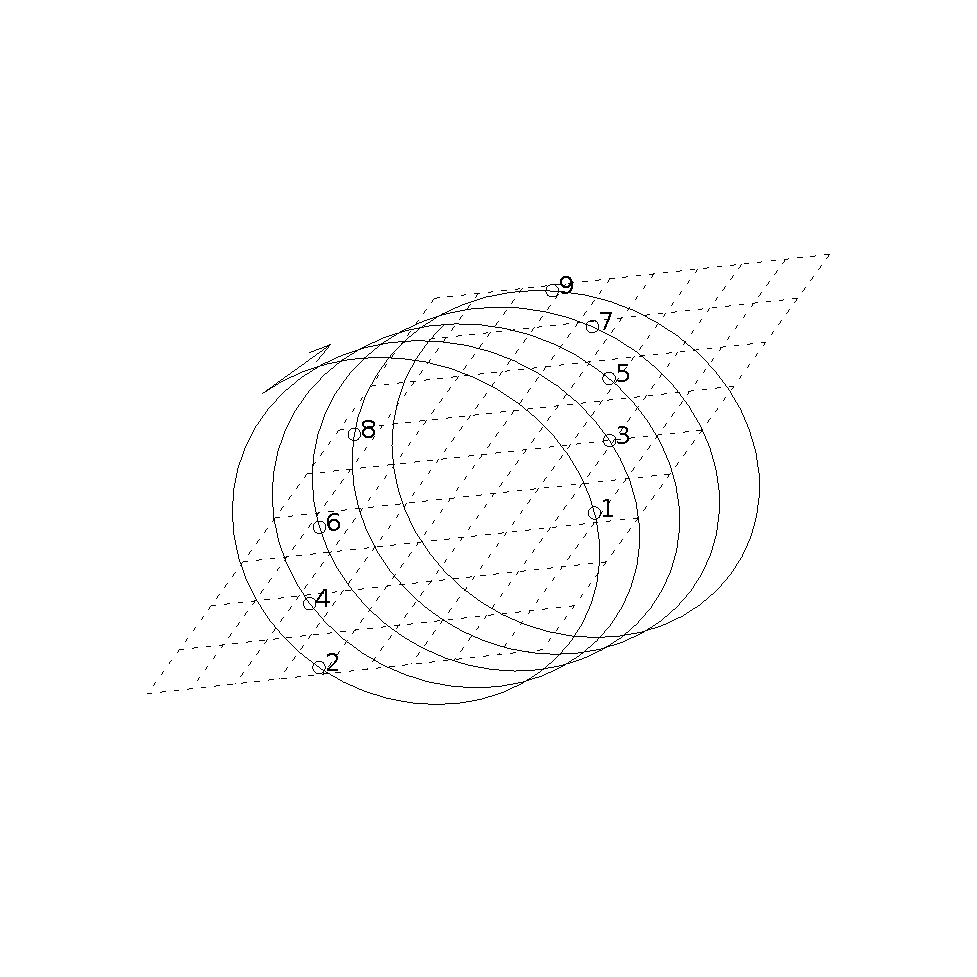
\includegraphics[trim={2.2cm 4cm 2cm 4cm},clip,width=.5,width=\textwidth]{images/arttrack/helix.eps}
         \caption{Винтовая линия, плоскость и точки пересечения в порядке
         заданном параметром $t$.}
         \label{fig:helixPlaneProblem}
     \end{subfigure}
     \hfill
     \begin{subfigure}[b]{0.6\textwidth}
         \centering
         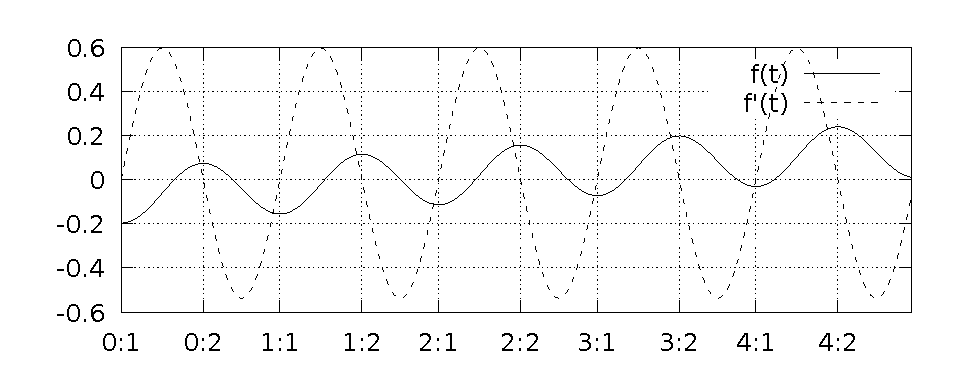
\includegraphics[width=\textwidth]{images/arttrack/helix-plane-func.eps}
         \caption{График функции проекции винтовой линии на нормаль плоскости.
         Отметки на горизонтальной оси соответствуют номеру периода и номеру
         экстремума в периоде.}
         \label{fig:hlxPlaneFuncAndDeriv}
     \end{subfigure}
        \caption{Изображение винтовой линии пересекающей плоскость и точек
            пересечения найденных при помощи численного метода в участках
            заданных \eqref{eq:helixPlaneExtrema}.}
        \label{fig:helixPlaneProblem}
\end{figure}

Для траектории заданной винтовой линией потребуется привлекать
численные методы, поскольку подстановка пропагатора \eqref{eq:helixMovement}
в уравнение плоскости приводит к трансцендентному уравнению с
произвольным числом корней
вида~$A \cdot \sin \theta + B \cdot \cos \theta + C \cdot \theta + D = 0$.
Участки монотонности этого трансцендентного уравнения заются двумя экстремумами
функции~\eqref{eq:helixMovement}:
\begin{equation}
    \theta_{1,2} = \pm \arcsin \frac{C}{\sqrt{A^2 + B^2}} - \arctan{\frac{B}{A}},
    \label{eq:helixPlaneExtrema}
\end{equation}
где $A = (\delta \vec{h} + \vec{t}_0) \cdot \vec{n}_p$,
$B = \alpha \vec{n}_p \cdot \vec{n}_0$, $C = \delta \vec{h} \cdot \vec{n}_p$.

Полностью, алгоритм отыскания пересечения винтовой линии
заданной~\eqref{eq:helixMovement} и плоскости выглядит следующим образом:
\begin{enumerate}
    \item Для заданного магнитного поля $\vec{B}$ импульса~$\vec{p}$ и
    заряда~$q$ частицы, отыскать экстремальные точки проекции касательного
    вектора на нормаль заданной плоскости~$\vec{n}_p$
    согласно~\eqref{eq:helixPlaneExtrema}, где $s > s_0$.
    \item Если корни \eqref{eq:helixPlaneExtrema} не определены (случай
    ориентации плоскости перпендикулярно полю), отыскание пересечения можно
    произвести численным методон последовательных приближений (напр. методом
    Ньютона), начиная с $s_0$.
    \item Подстановкой~\eqref{eq:helixPlaneExtrema} в~\eqref{eq:helixMovement}
    определить участки перемены знака и использовать в них численный метод
    отыскания нуля на отрезке (напр. дихотомий). При этом, если подстановка
    корней не приводит к уменьшению абсолютной величины среднего значения
    функции в течении двух последовательных периодов, считать, что пересечений
    с плоскостью нет (частица удаляется от плоскости).
\end{enumerate}
Реализация такого алгоритма должна предусматривать случай когда ось винтовой
линии
\begin{equation}
    \vec{l}(s) = \vec{r}_0 + \delta \vec{h} s + n_0 \alpha / K.
    \label{eq:helixAxis}
\end{equation}
параллельна плоскости --- то есть число корней~\eqref{eq:helixPlaneExtrema}
бесконечно.

Результат работы такого алгоритма представлен на рисунке~\ref{fig:helixPlaneProblem}.

\subsubsection{Определение локальных координат}

\begin{center}
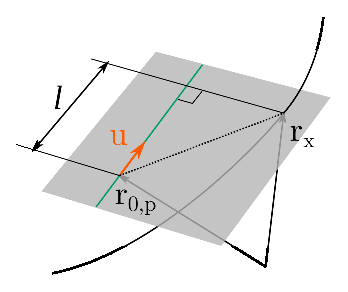
\includegraphics[width=.5\textwidth]{images/arttrack/arttrack-u-measurement.eps}
\end{center}

\subsubsection{Реализация}

\begin{figure}[ht]
    \centering
    \subfloat[Фронтальный вид]{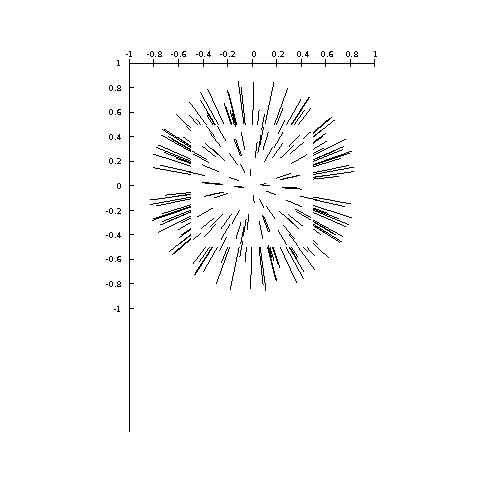
\includegraphics[trim={0 3cm 0 0},clip,width=.5\textwidth]{images/arttrack/box-in-sphere-ortho.eps}}
    % ^^^ trim={0 3cm 0 0},clip,
    \subfloat[Ортографическая проекция]{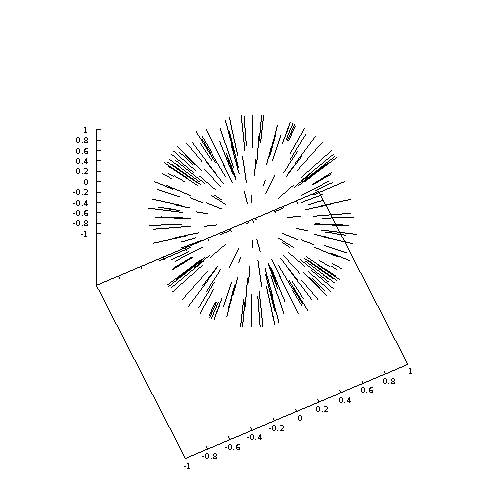
\includegraphics[width=.33\textwidth]{images/arttrack/box-in-sphere.eps}}
    \caption{Визуализации различных тестов.}
    \label{fig:boxInSphere}
\end{figure}

         % Глава 2
\chapter{Реализация программного комплекса NA64}

Данная глава посвящена описанию реализации
программного комплекса и соответствующим физическим результатам,
полученным с применением описанных ранее методов.

\begin{comment}
Реконструкция данных представляет собой преобразование
сигналов детекторов в рамках одной и той же согласованной модели,
с применением калибровочной информации.

Применение конкурирующих численных методов и их динамическая композиция
могут быть обобщены в рамках машины конечных состояний, которые применяются,
в частности, к задаче аппроксимации амплитудной функции сигналов калориметров
или реконструкции треков с проверкой конкурирующих гипотез.

С практической точки зрения, многие элементарные
варианты использования могут быть эффективно обобщены
в рамках специализированных выразительных средств (искусственных
языков). В частности, они обеспечивают мощные
выразительные средства для повторяющихся задач:
выбор детекторов, запросы к модели события, описание калибровочных
данных.

Выбор форматов данных должен быть обоснован в рамках заданных
архитектурных инвариантов, фиксируя протоколы обмена данными между
основными компонентами.
\end{comment}

%В главе рассмотрены реализации компонент программного комплекса,
%выполняющих конкретные задачи в рамках предложенной архитектурной
%концепции. Глава завершается изложением физических результатов
%полученных с применением этих средств.

\section{Динамические машины состояний}

Для решения задач выбора конкурирующих гипотез -- таких, как разделение
амплитудных импульсов во времени или выбор между гипотезами о
треке частицы,
%в рамках подхода быстрого прототипирования,
целесообразно прибегнуть к высокому уровню общности,
поскольку по мере появления новых детекторов и считывающей аппаратуры,
тестирования и разработки новых методов реконструкции сигналов,
необходимо производить исследование поведения существующих алгоритмов,
производить оптимизацию параметров и часто изменять систему.

Истинная функция отклика подвержена влиянию многих факторов: существенно
зависит от считывающей аппаратуры и изменяется в зависимости от вещества
рабочего объёма детектора.
%Используемая в качестве приближения
%\emph{модельная функция} $f(t,\vec{p})$ --- аппроксимация амплитуды в момент
%времени $t$ праметризуемая параметрами $\vec{p}$
С некоторыми допущениями, для реконструкции
можно применять упрощённую модель или быстрый алгоритм реконструкции с
потерей точности там, где ошибки не так важны как средняя картина
наблюдаемых распределений.

Например, при
мониторировании детекторов во время набора данных.
Напротив, для задач анализа целесообразно
стремиться к наиболее правдоподобной модели -- например, для улучшения
разрешения при реконструкции ливней в калориметрах, поскольку
малые амплитуды на периферии ливня приобретают большое значение
в дискриминационных логических схемах.

%Важно отметить, что помимо задачи
%разрешения откликов САЦП, общая постановка задачи справедлива и для
%задачи реконструкции треков, которая в общем формулируется чаще всего
Другим примером является реконструкция треков, сформулированная
как задача минимизации функционала статистики
$\chi^2$ % = \sum\limits_i (f((t_i,\vec{p}) - r_i)/\sigma_i)^2$
от некоторой (в общем -- нелинейной, необязательно аналитической)
функции параметризации
трека $f(t,\vec{p})$ по отношению к выбранным наборам показаний
координатно-чувствительных детекторов $\vec{r}_i$. При этом
%, как правило, при больших загрузках детекторов,
%типичных для современных экспериментов с большой светимостью,
для разрешения возникающих неоднозначностей применяются различные
алгоритмы отбора: в рамках общей задачи поиска трека~(англ. \emph{track finding})
поиск может производиться по известным пространственным
шаблонам~(англ. \emph{pre-patterning}),
на основе пространственных биекций,
разбиения на KD-дерево, и т.д. ~\cite{MankelTracking, artificial-retina-tracking-lhc}
Такие алгоритмы обычно дают довольно грубое
приближение для более высокоуровневого алгоритма аппроксимации трека,
существенно снижающее набор входных значений по отношению к прямому
комбинаторному перебору.

\subsection{Варианты использования}

Пусть \emph{модель} --- математическая
функция $f(x,\vec{p})$, определённая в зависимости от некоторого
аргумента $x_i$ и вектора параметров $\vec{p}$. Целью
\emph{процедуры минимизации} является отыскание таких параметров $\vec{p}$
при которых достигается наилучшее соответствие набору входных данных $y_i$
согласно некоторой метрике (реализация принципа максимального правдоподобия).
При этом под отдельной программной процедурой далее понимается
формализованный алгоритм осуществляющий преобразование вектора параметров
модели~$P(\vec{p}_a) = \vec{p}_b$ (т.е. не обязательно минимизация).
%Символически, можно записать, что для некоторой метрики $\mathbb{M}$
%преобразование заданное процедурой $P$
%т.е. целью процедуры как преобразования $P[\vec{p}_a] \rightarrow \vec{p}_b$
%является отыскание таких $\vec{p}_b$ при которых достигается
%условие~$\text{min}()$

Индуктивно выделяются как минимум следующие основные варианты
использования системы, с точки зрения пользовательского кода,
расширяющие исходный сценарий применения процедуры к
программной модели:
\begin{itemize}
    \item Выбор и \emph{установка начальных значений} параметров $\vec{p}$
    на основе исходной выборки значений $x_i$. Этот вариант
    подразумевает предварительное вычисление начальных приближений
    на основе широкого набора параметров регулирующих поведение
    поисковых алгоритмов.
    \item \emph{Применение алгоритма численной минимизации}. Помимо
    \acrshort{lms} сюда относится, например, фильтр Калмана в его
    различных модификациях,
    и в целом задачи линейного программирования допускающие выражение
    в виде линейно-алгебраических операций над модельной функцией с
    фиксированным набором параметров.
    \item Элементарный вариант использования состоит в прямом
    \emph{изменении параметров модельной функции}. Такой этап может быть
    полезен, например, при искусственном введении возмущения в
    линейных алгоритмах минимизации с целью преодоления локальных
    минимумов.
    \item \emph{Применение процедур к отдельным элементам} и подразумеваемая
    в таком случае \emph{декомпозиция модели} может понадобиться,
    когда с точки зрения численной процедуры минимизации, модель может
    быть тем или иным образом разложена (факторизована) на набор более
    элементарных независимых моделей, к каждой из которых необходимо
    применить определённый набор процедур. Например: аппроксимация
    функции отклика для значительно разнесённых во времени пиков,
    аппроксимация трека частицы на линейных участках в отсутствии
    магнитного поля, и т.д.
    \item Для \emph{сопоставления результатов} аппроксимации между
    конкурентными методами посредством определённой метрики (в частности,
    выбор наилучшей гипотезы о треке на основании $\chi^2$), необходима
    соответствующая формализация, делегирующая выполнение
    конкретной реализации компаратора.
    \item В тех случаях, когда метрика не может быть определена для
    моделей, и основным результатом является логическое условие применимости
    процедуры, целесообразно выделить вариант использования перебирающий
    процедуры до тех пор, пока очередной вариант не будет
    выполнен успешно (\emph{выбор подходящей модели}).
    \item Наконец, \emph{выбор или замена модельной функции} в рамках
    такого уровня общности тоже представляет собой вариант использования.
\end{itemize}

\begin{figure}
    \centering
    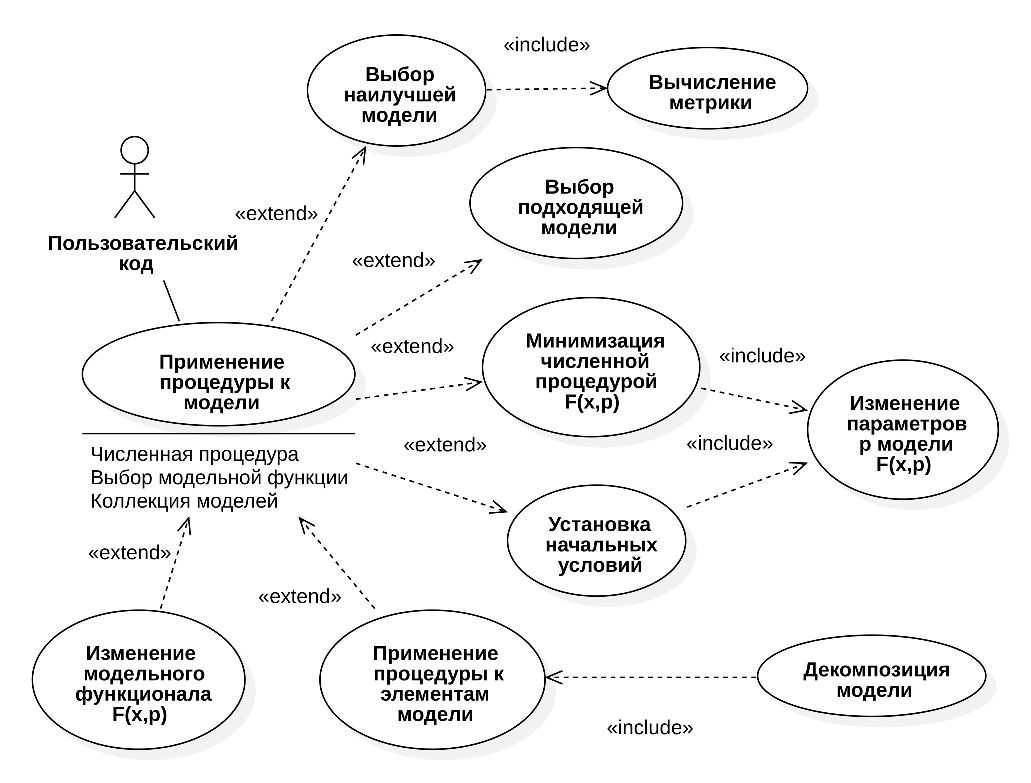
\includegraphics[width=0.95\linewidth]{images/umff-usecase-diagram-02.eps}
    \caption{Диаграмма вариантов использования программной библиотеки для
    решения задач численной минимизации с расширенной логикой (ветвление,
    сопоставление, перебор).}
    \label{fig:umff-usecases}
\end{figure}

Рисунок \ref{fig:umff-usecases} иллюстрирует отношения между перечисленными вариантами
использования.

\subsection{Компоненты машины конечных состояний}

Описанная структура вариантов использования подразумевает наличие по крайней мере
следующих элементов обобщённого поведения:
\begin{itemize}
    \item Составная процедура содержащая набор более простых процедур,
    делегирующая выполнение этому набору, и завершающаяся результатом
    отобранным согласно некоторому правилу (\emph{competing}).
    \item Составная процедура осуществляющая декомпозицию модели в тех случаях,
    когда модель это позволяет, инкапсулирующая набор более простых процедур,
    и применяющая этот набор по отдельности к каждому элементу
    декомпозиции~(\emph{breakdown}).
    \item Последовательность процедур в которой последующая применяется только
    в том случае, если текущая завершилась не успешно
    (\emph{fallback}).
    %Рисунок \ref{fig:fallback-example} содержит
    %пример машины конечных состояний, в которой применение процедуры
    %делегируется, а валидация выполняется самим элементом.
\end{itemize}

Этот базовый набор логических элементов позволяет конструировать сложные
условные последовательности, которые наиболее просто представить в виде
машин конечных состояний. В таких машинах состояниям отвечает
модель~($m_i:=f(x_i,\vec{p})$),
а переходам соответствует процедура~$P(\vec{p}_a) = \vec{p_b}$.

Техническое описание и спецификации вынесены в приложение~\ref{appendix:fsm-machine-prog}.

\subsection{Восстановление амплитудных сигналов}

На рисунке~\ref{fig:sadc-wf-fitting-example} приведён пример
восстановленного отклика ячейки электромагнитного калориметра от двух
импульсов слабо (не более чем на ширину) разнесённых во времени.
Пунктирной линией с коротким штрихом
изображён график конечно-разностной аппроксимации первой производной
по точкам сигнала, сплошными серыми линиями изображён результат
подгонки -- для отдельных импульсов и их восстановленная сумма.
Пунктирная линия с длинным штрихом отвечает начальным условиям.
%время в наносекундах против амплитуды в относительных единицах

\begin{figure}[ht]
    \centering
    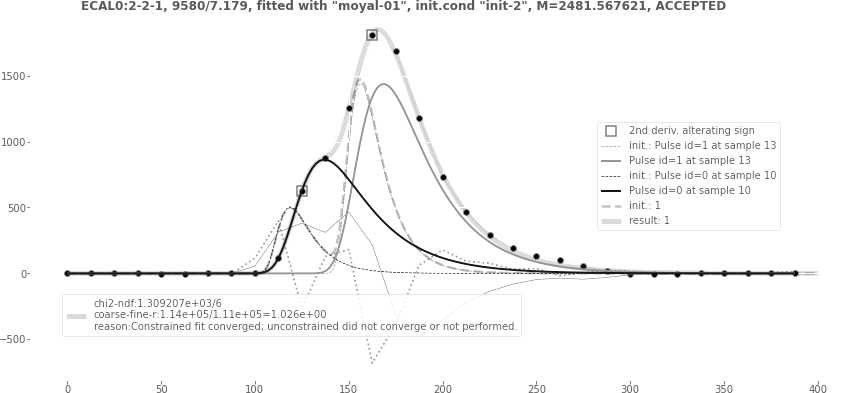
\includegraphics[width=0.99\linewidth]{images//illustrative/waveform-fit-result-example.png}
    \caption{Пример восстановления сигнала от двух частиц с малой временным
    интервалом}
    \label{fig:sadc-wf-fitting-example}
\end{figure}

Этот случай имеет большое значение в отношении физической картины,
поскольку подобную сигнатуру часто дают мюоны от
распадающихся в голове канала
пионов $\pi^{\pm} \rightarrow \mu^{\pm} \nu_\mu$ 
и каонов $K^{\pm} \rightarrow \mu^{\pm} \nu_\mu$,
или мюонные пары от реакций $\gamma Z \rightarrow Z \mu^{+}\mu^{-}$.

Наивный алгоритм построенный на выделении абсолютного максимума
не способен обнаружить первый импульс от слабоэнергетической частицы,
поскольку первый импульс вообще не даёт максимума. 

Второй пик распознаётся алгоритмом отыскания
импульсов, опирающимся на сигнатуру чередования роста и спада
функции. Аппроксимация моделью затем производится с учётом
индивидуальных особенностей ячейки, поскольку в общем случае
подгонка параметров модели в данной картине допускает неоднозначность
результатов. Кроме того, из-за присутствующей неоднозначности
весьма вероятна сходимость процедуры подгонки к локальному минимуму,
что решается посредством одновременного рассмотрения
нескольких конкурирующих гипотез (competing).


\section{Восстановление треков частиц}

Трекинг в NA64 необходим для определения энергии и идентификации
типа частиц попадающих в электромагнитный калориметр или
покидающих его. Важной особенностью экспериментов на фиксированной мишени
упрощающей рассмотрение треков частиц является допущение о
прямолинейности истинных траекторий частиц в отсутствии магнитного
поля и плотного вещества. Так в постановке для изучения электромагнитных
ливней инициированных электроном трекер
представляет собой двухплечевой спектрометр составленный
из нескольких газовых детекторов, расположенных по оси пучка с
условно-прямолинейными участками траектории до и после магнита,
перед массивным электромагнитным калориметром.
%с совокупным \emph{вкладом ??}.
Для мюонной постановки трекер дополнительно оснащается станциями
BMS (англ. \emph{beam momentum station}) в голове канала.
После калориметра устанавливается дополнительный
спектрометр представленный отклоняющим дипольным магнитом и дополнительными
станциями MicroMega и Straw с увеличенным
угловым аксептансом для идентификации частиц покидающих ECAL.

В целом, высокое пространственное разрешение
и сравнительно слабая оснащённость детекторами (по две или три станции на плечо,
выбранная, с тем чтобы минимизировать ионизационные потери и рассеяние), а
так же применение детекторов с гальванически связанными каналами (MicroMega)
обуславливают важные частные особенности трекера~NA64:
\begin{enumerate}
    \item Низкая заселённость за исключением второго спектрометра в мюонной
    постановке. В постановке с электронным или адронным пучком среднее
    число треков на событие -- $1{,}4$.
    \item Линейная протяжённость в десятки метров при сравнительно малой площади
    чувствительной поверхности детекторов в сотню $\text{см}^2$.
    \item Присутствие ложных срабатываний в MicroMega из-за гальванического
    соединения анодных полос (коммутации в одну сигнальную линию).
\end{enumerate}

С одной стороны эти особенности создают существенные методические
ограничения: невозможность эффективно использовать гало пучка для
выравнивания, и невозможность эффективно покрыть трекер в голове
канала расфокусированным пучком
для выравнивания и изучения эффективности трекера.

С другой стороны, при сравнительно высоком пространственном разрешении
трекера, дающим энергетическое разрешение не хуже $1~\text{ГэВ}$,
и сам трекинг, и геометрическое выравнивание детекторов на его основе
вносят не столь существенный вклад в систематическую ошибку эксперимента.

\subsection{Измерения микроструктурных детекторов}

Оцифрованный сигнал с микроструктурных детекторов GEM и MicroMega представляет
собой кортеж из трёх чисел отвечающих измерениям амплитуды напряжения на переднем
фронте токового импульса соответствующего стрипа (металлической полоски на считывающей
поверхности детектора), как показано на рисунке~\ref{fig:apv-pulse-sampling}.

\begin{figure}
    \centering
    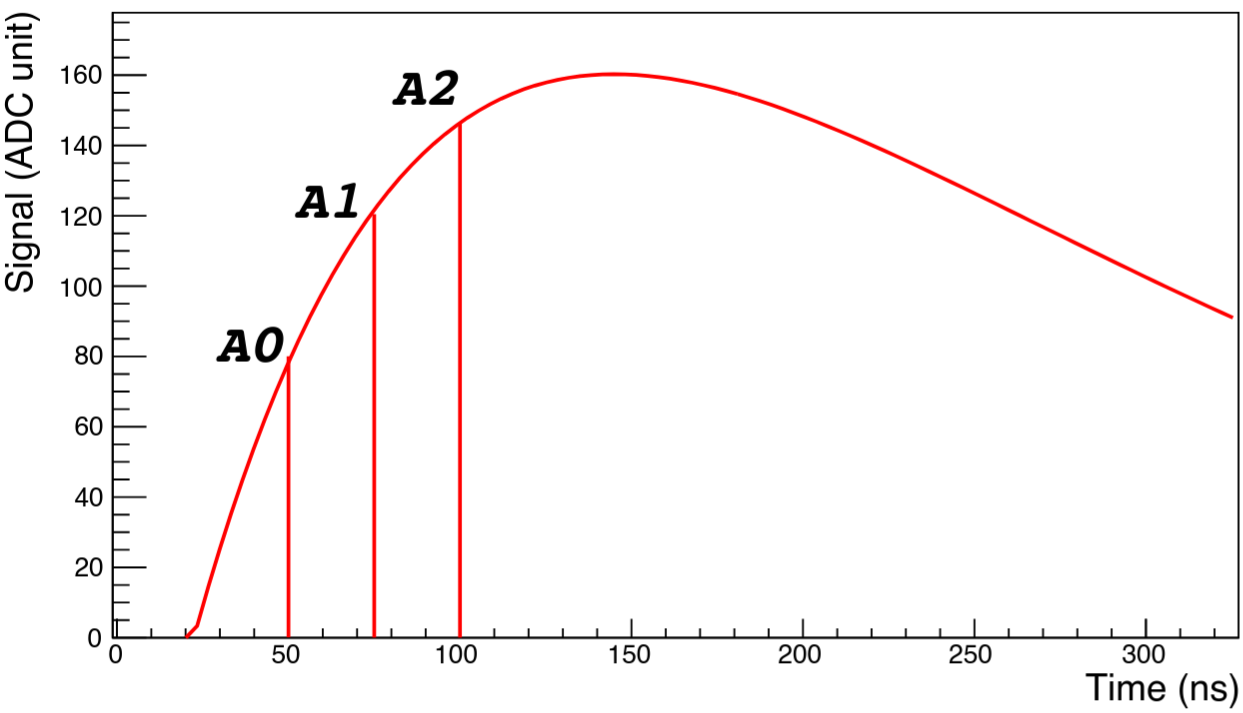
\includegraphics[width=0.45\linewidth]{images//illustrative/mm-amps.png}
    \caption{Сэмплирование переднего фронта сигнала с одного канала
    микроструктурного детектора~\cite{na64-BANERJEE201872}}
    \label{fig:apv-pulse-sampling}
\end{figure}

В рабочем режиме детектора средняя точка отвечает критерию постоянной
доле~(англ. \emph{constant fraction}~\cite{grupenDetectors2008}) и её
относительное временное смещение не зависит от
амплитуды. Поскольку у элементов входных каскадов считывающей электроники присутствует
разброс параметров, вывод детектора в рабочий режим требует
подстройки фазы синхронизирующего импульса~\acrshort{sadc}.

Для этого строится гистограмма отношений
амплитуд $r_{02}=A_0/A_2$ и $r_{12}=A_1/A_2$,
пример которой приведён на рисунке~\ref{fig:banana-histogram}. Калибровка 
заключается в выборе дискриминирующего условия на основе такого
распределения, выражающаяся в параметризованном неравенстве (обычно,
включающае полигональную фигуру, полиномы, сплайны или кривые Безье).
Таким образом исключаются паразитные
амплитуды.

\begin{figure}
    \centering
    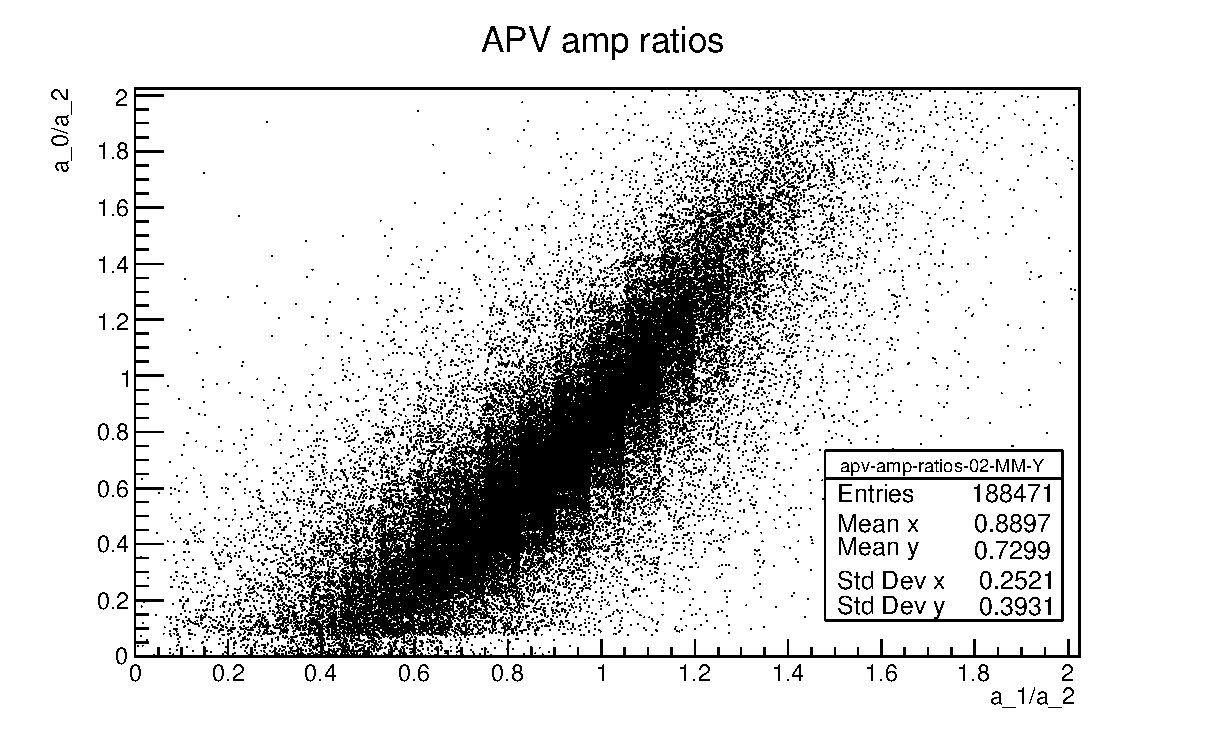
\includegraphics[width=0.45\linewidth]{images/illustrative/banana-example.eps}
    \caption{Пример распределения отношения амплитуд $r_{02}$ и $r_{12}$ переднего
    фронта сигнала микроструктурного детектора}
    \label{fig:banana-histogram}
\end{figure}

\subsection{Измерения от тонкостенных зарядовых трубок}

%Станции тонкостенных газоразрядных трубок предоставляют информацию
%о времени развития электронной лавины $t'$ в рабочем объёме конкретной
%трубки относительно времени срабатывания триггера. В $t'$ включено
%время пролёта частицы до трубки $\delta t$, которое для большинства
%релятивистских частиц (мюонов и электронов) принимается постоянным.
%Так, например, времяпролётная разница на дистанции в десять метров
%для электронов в $1~\text{ГэВ}$ и $100~\text{ГэВ}$ составляет
%менее $1~\text{пс}$, для мюонов -- менее $200~\text{пс}$, в то время
%как характерное время дрейфа лавины в трубке обычно составляет десятки
%наносекунд -- $20~\text{нс}$ для трубок диаметром $2~\text{мм}$
%и $50~\text{нс}$ для трубок $6~\text{мм}$. При принципиально-достижимом
%координатном разрешении в детекторах такого типа в $200~\text{мкм}$
%эта разница во временах для лептонов высоких энергий несущественна.
Станции тонкостенных газоразрядных трубок регистрируют время развития
электронной лавины $t'$ в рабочем объёме каждой трубки относительно
сигнала триггера. В это время включено также запаздывание
частицы $\delta t$, которое для большинства релятивистских частиц
практически постоянно. Так, например, различие
во времени пролёта на расстоянии десяти метров между электронами с
энергией $1~\text{ГэВ}$ и $100~\text{ГэВ}$ составляет менее $1~\text{пс}$,
а для мюонов~-- менее $200~\text{пс}$, тогда как характерное время
дрейфа лавины в трубке находится на уровне десятков наносекунд:
около $20~\text{нс}$ для трубок диаметром $2~\text{мм}$ и порядка
$50~\text{нс}$ для трубок диаметром $6~\text{мм}$. При достижимом
координатном разрешении таких детекторов на уровне менее $200~\text{мкм}$,
указанные различия во времени пролёта для лептонов высоких энергий
не имеют существенного значения.

%По этой причине $t'$ определяется главным образом временем $T$ дрейфа
%электронной лавины в разрядном промежутке трубки от ближайшей точки
%ионизации до катодной проволоки с расстоянием $R$, которое в свою очередь
%в наибольшей степени зависит от давления и плотности газовой смеси.
Таким образом, величина $t'$ определяется главным образом временем $T$
дрейфа электронов в разрядном промежутке трубки от ближайшей точки
ионизации до катодной проволоки.

%Таким образом зависимость $R(T)$, хотя и имеет нелинейный характер,
%хорошо поддаётся аппроксимации различными аналитическими моделями.
%Параметры такой модели и составляют необходимую калибровочную
%информацию применяемую при определении радиуса
%изохроной цилиндрической поверхности задаваемой временем срабатывания~$T$.
Функция $R(T)$ имеет нелинейный характер, однако хорошо аппроксимируется
различными аналитическими моделями. Параметры такой аппроксимации и
составляют необходимую калибровочную информацию, используемую при
определении радиуса изохронной цилиндрической поверхности, соответствующей
данному времени срабатывания~$T$.

На рисунке~\ref{fig:straws-rt} изображена гистограмма полученная для
трубки диаметром $6~\text{мм}$, находящейся
позади адронного калориметра с наложенными поверх гистограмм аппроксимациями
зависимости $R(T)$.
%\begin{figure}[ht]
%    \centering
%    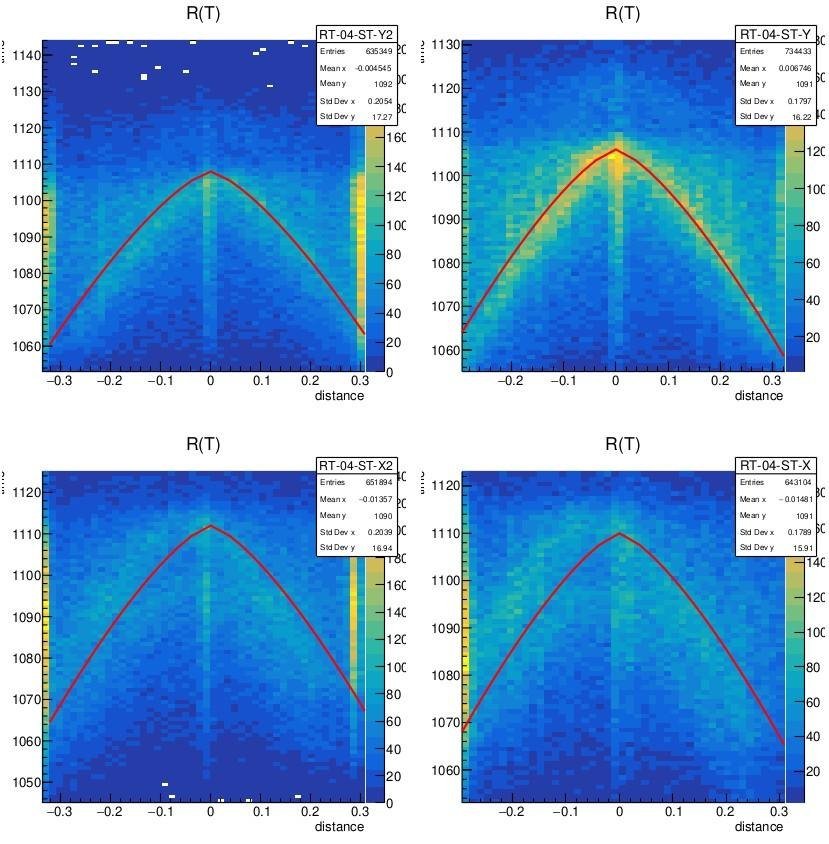
\includegraphics[width=0.95\linewidth]{images/illustrative/ST-RT.jpg}
%    \caption{Распределение $R(T)$ для нескольких трубок станции ST
%    диаметром $6~\text{мм}$ (ось времени инверирована)}
%    \label{fig:straws-rt}
%\end{figure}
\begin{figure}
    \centering
    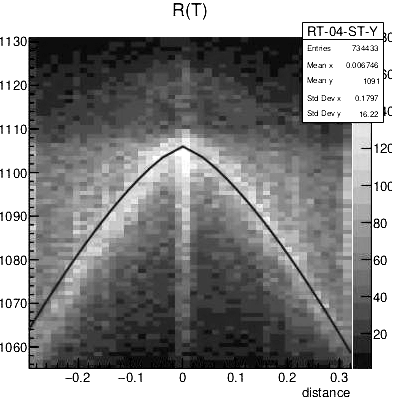
\includegraphics[width=0.33\linewidth]{images//illustrative/ST-RT-single-mono.png}
    \caption{Распределение $R(T)$ для нескольких трубок станции ST
    диаметром $6~\text{мм}$
    %, $R$ в мм, время в относительных единицах, ось времени инверирована
    }
    \label{fig:straws-rt}
\end{figure}
Большое количество срабатываний отстоящих от основной линии обусловлено
высоким фоном от вторичных частиц.

%Хотя определение радиуса изохронной поверхности таким образом представляет
%собой простую задачу (реализуемую при помощи единственного обработчика,
%применяющего калибровочные данные), последующее использование этой
%информации в
%алгоритмах трекинга требует привлечения нетривиальных
%алгоритмов либо на этапе предварительного поиска треков, либо
%в процессе подгонки параметров модели трека. В простейшем случае, проводят
%плоскость через оси трубок в одной координатной проекции, и отмечают
%линии пересечения изохронной поверхности с этой плоскостью. Получившиеся
%линии таким образом являются геометрическим местом возможного пересечения
%траектории частицы с плоскостью детектора с фиксированным разрешением.
%Поскольку для одной трубки таких линий образуется две, одной трубки
%недостаточно для определения координат частиц в одной проекции.
Хотя определение радиуса изохронной поверхности в таком подходе
представляет собой относительно простую задачу (реализуемую с помощью
единственного обработчика, использующего калибровочные данные),
дальнейшее применение этой информации в алгоритмах трекинга требует
привлечения более сложных методов -- как на этапе предварительного
поиска треков, так и при подгонке параметров модели трека. 

В простейшем случае через оси трубок в одной координатной проекции
проводится плоскость, и фиксируются линии пересечения изохронной
поверхности с этой плоскостью. Эти линии образуют геометрическое
место возможных точек пересечения траектории частицы с плоскостью
детектора при данном временном разрешении. Поскольку для одной трубки
возникают две такие линии, её информации недостаточно для определения
координаты частицы в одной проекции. Тем не менее, рассматривая показания
трековых детекторов в совокупности зачастую удаётся разрешить
возникающие неоднозначности. На рисунке~\ref{fig:evdisplay-new}
показана проекция пространственных примитивов изображающих
чувствительные объёмы детекторов MicroMega и станции трубок
совместно с допустимыми пределами разрешений (изображены
шириной $5\sigma$).

\begin{figure}[ht]
    \centerfloat{
        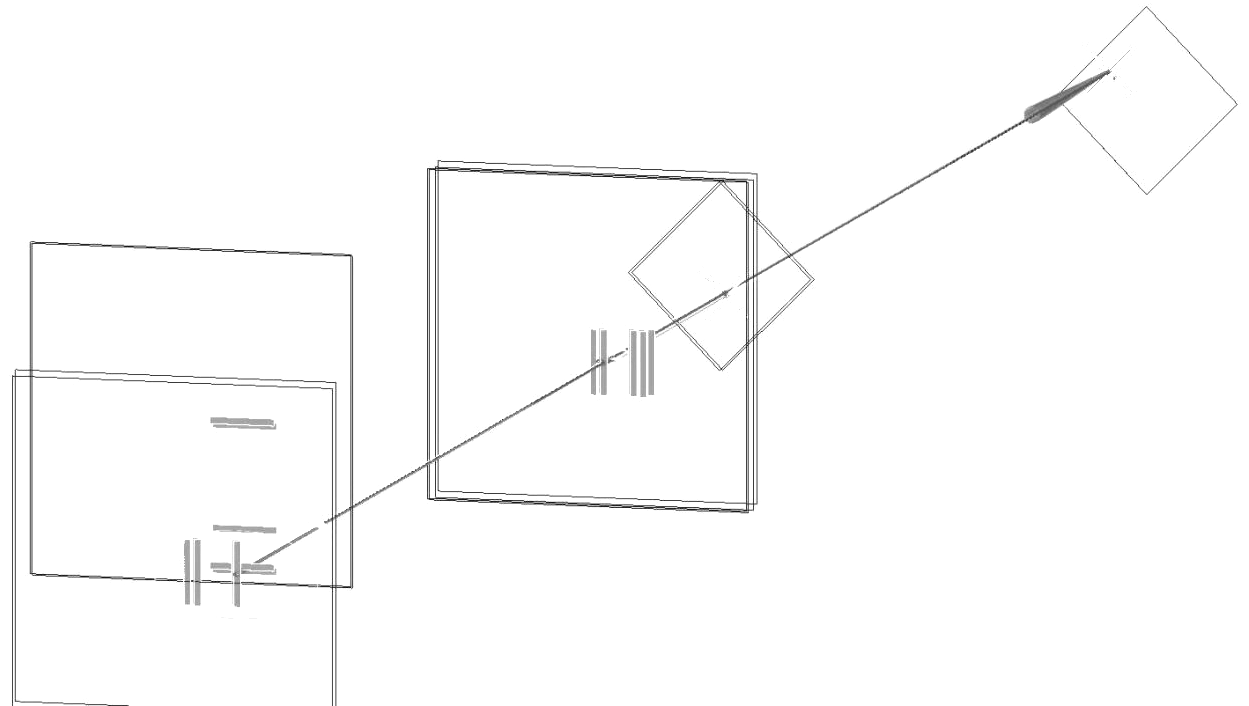
\includegraphics[width=0.5\linewidth]{images//illustrative/ST-evdisp-mono.png}
    }
    \caption{Реконструкция треков по показаниям MicroMega (повёрнуты на $45^{\circ}$)
    со станциями тонкостенных разрядных трубок с изображением
    координатных разрешений и гипотезы трека с ковариационными конусами}
    \label{fig:evdisplay-new}
\end{figure}

%\begin{figure}
%    \centering
%    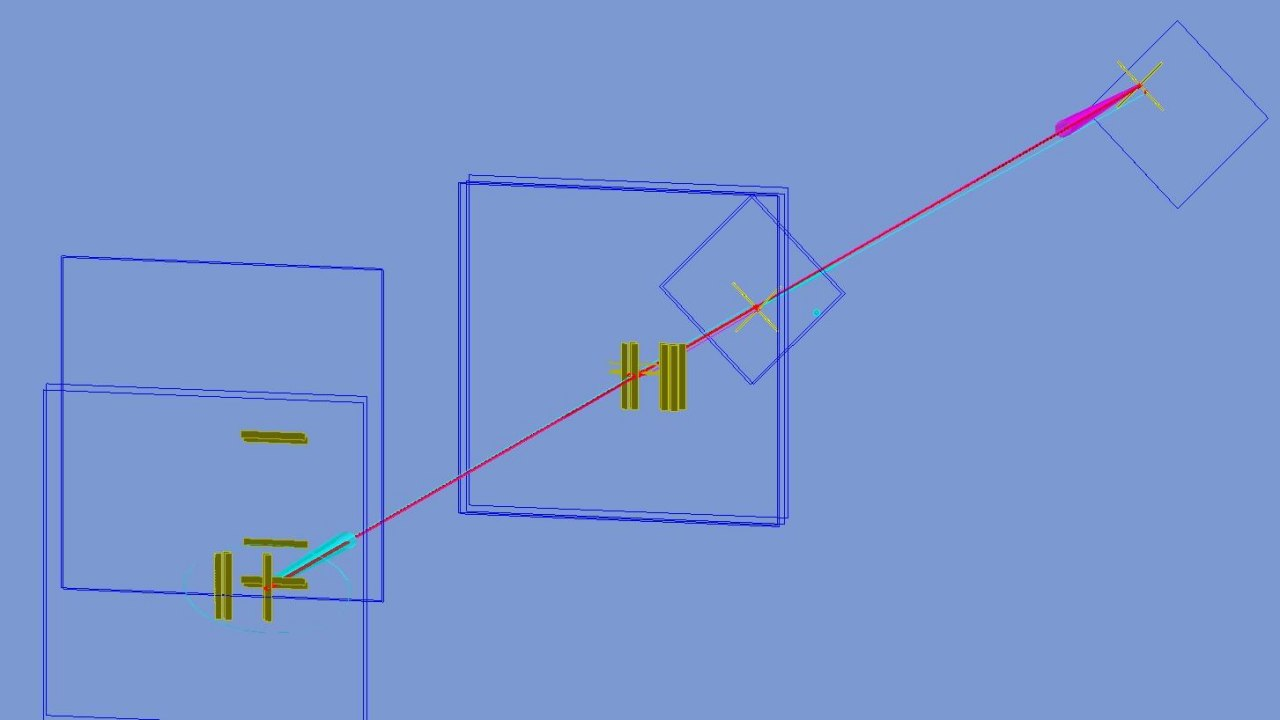
\includegraphics[width=0.5\linewidth]{images/illustrative/ST-evdisp.jpg}
%    \caption{Реконструкция треков в SPA}
%    \label{fig:evdisplay-new}
%\end{figure}

Возможны и более сложные алгоритмы реконструкции, учитывающие
трёхмерную структуру изохронных поверхностей в рамках одной станции
тонкостенных трубок~\cite{straws-peshekhonov2015}.

\subsection{Алгоритмы аппроксимация треков}

Классическая задача восстановления трека по измеренным
координатам в NA64 решалась различными методами.
Наиболее актуальным является фильтр Калмана~\cite{kalman-1960},
реализованный библиотекой GenFit2~\cite{Genfit2_Rauch_2015}
в различных редакциях и с дополнениями оригинального алгоритма, из которых
наибольший практический интерес в контексте NA64
представляют
\acrshort{daf} (англ. \emph{deterministing annealing filter}~\cite{daf-track-fitting})
и \acrshort{krf}
(англ. \emph{Kalman filter with reference track}~\cite{krf-kalman-w-reference-track}).

Для подгонки параметров модели треков в условиях сложной геометрии
применяется \acrshort{krf}.
Его особенность по сравнению с оригинальным алгоритмом Калмана
состоит в том, что линеаризация функции описывающей движение
частицы выполняется не в малой окрестности координатного измерения, а
относительно заранее заданной опорной траектории,
обновляемой затем в несколько итераций. Этот приём позволяет снизить
систематические ошибки при аппроксимации трека в
неоднородном магнитном поле, с учётом эффектов множественного
рассеяния (например, при трассировке участка трека через калориметр).
Использование данного метода оправданно в сочетании с алгоритмами
поиска треков, которые задают разумное начальное приближение
для опорной траектории. % -- таких, как CATS~\cite{catsc-nim}.

\acrshort{daf} решает иную задачу: выбор согласованного подмножества
измерений в условиях неоднозначностей и шумов. В
его основу положено назначение весов отдельным координатным измерениям
с последующим итеративным обновлением. Таким образом, вначале все
измерения вносят вклад в гипотезу о треке частицы, затем, в течение
нескольких итераций, веса
асимптотически сходятся к самосогласованной гипотезе.
В пределе это приводит к отбору хитов, принадлежащих
правдоподобной гипотезе с эффективным исключением ложных
срабатываний.

\subsection{Задача предварительного поиска треков}

%Задача предварительного поиска треков (англ. \emph{pattern recognition})
%состоит в выборе таких комбинаций пространственных объектов соответствующих
%отдельным измерениям, которые с заданной
%степенью правдоподобия могут образовывать трек частицы.
Задача предварительного поиска треков % (англ. \emph{pattern recognition})
заключается в отборе таких комбинаций пространственных объектов,
соответствующих отдельным измерениям детектора, которые с заданной
степенью правдоподобия могут образовывать трек частицы.


%Среди множества существующих на сегодняшний день алгоритмов предварительного
%поиска треков~\cite{MankelTracking}, интерес представляет алгоритм
%CATS~\cite{catsc-JINR, catsc-discrete, catsc-nim, catsc-disto},
%(англ. \emph{cellular automata track search} -- в разное время авторы
%публиковали его формализацию в терминах <<эластичных>> нейронных сетей,
%и клеточных автоматов), который допускает весьма общую
%формулировку в силу независимости по отношению к конкретным
%геометрическим свойствам входных данных.
Среди многочисленных алгоритмов предварительного поиска~\cite{MankelTracking}
интерес представляет метод CATS\footnote{В различных публикациях
он излагался как в терминах <<эластичных>> нейронных сетей,
так и в формализме клеточных автоматов.}
(англ. \emph{cellular automata track search})~\cite{catsc-JINR, catsc-discrete, catsc-nim, catsc-disto}.
Алгоритм допускает весьма общую формулировку в силу независимости по
отношению к конкретным геометрическим свойствам входных данных.

Формально задача, решаемая алгоритмом, может быть представлена следующим образом.
Пусть имеется
набор объектов $h_1,h_2, ...h_n$ (англ. \emph{hit}). Требуется найти такие
последовательности $(h_i,h_j,...h_m)$, для которых любая тройка
элементов $(h_{i-1},h_{i},h_{i+1})$ удовлетворяет заданному
условию $F(h_{i-1},h_{i},h_{i+1})=1$.
Основная идея состоит в эффективной стратегии обхода
объектов~$h$, позволяющей в большинстве случаев избежать прямого перебора
всех возможных комбинаций. Для этого алгоритм опирается на
топологическую информацию о <<слоях>> связанных с каждым
объектом~$h$. Каждому объекту сопоставляется
внутреннее состояние, обновляемых за конечно число итераций согласно
определённому правилу.

Пример работы алгоритма показан на рисунке~\ref{fig:catsc-nim},
где приведены начальное и конечное состояния графа для
синтетических данных.

\begin{figure}
    \centerfloat{
        \hfill
        \subcaptionbox{Начальное состояние}{
            \includegraphics[width=0.45\linewidth]{images//illustrative/catsc-quote-it1.png}}
        \hfill
        \subcaptionbox{Конечное состояние}{
            \includegraphics[width=0.45\linewidth]{images//illustrative/catsc-quote-it6.png}
        }
        \hfill
    }
    \legend{Слои отмечены пунктирными
    линиями, объекты $h$ изображены кругами, рёбра между парами
    объектов~--- сплошными линиями, а увеличенная толщина линии указывает
    на больший вес соответствующей пары.}
    \caption{Пример работы клеточного автомата CATS~\cite{catsc-nim}}
    \label{fig:catsc-nim}
\end{figure}

В простейшем случае, в качестве объектов $h$ выбираются пространственные
точки, а условием $F$ является условие на максимальный пространственный
между ними $F(h_{i-1},h_{i},h_{i+1}): \angle(h_{i-1}h_i) (h_i h_{i+1}) < \theta_{th}$.

В результате время работы алгоритма оказывается существенно ниже
прямого перебора, в худшем случае ($\theta_{th} =\pi$) имея
сложность $\mathcal{O}(Ln^3)$, где $L$ -- число слоёв,
и $n$ -- число объектов $h$. Практически, сложность регулируется
функцией-фильтром, и при трудоёмкости фильтра~$\mathcal{O}(1)$ алгоритм
имеет сложность $\mathcal{O}(Ln^2)$. Наивный перебор троек $h$
с фильтрующей функцией дающей в среднем $d$ объектов в следующем слое
имеет сложность $\mathcal{O}(n^3 d^{L-3})$. Без фильтрующей функции
максимальная сложность возрастает экспоненциально $\mathcal{O}(n^L)$,
однако главное преимущество CATS перед наивной реализацией состоит
в устранении экспоненциального роста памяти, необходимой для хранения
гипотез. Алгоритм сводит задачу к итеративному однонаправленному обходу
двунаправленного графа без рекурсии.

В оригинальных работах~\cite{catsc-JINR, catsc-discrete, catsc-nim, catsc-disto}
$h_i$ рассматриваются как пространственные точки $h_i:=\vec{r}_i$, или кортежи из
координат и времени $h_i:=(\vec{r}_i,t_i)$, в то время как алгоритм сам по себе
не подразумевает какого-то конкретного набора свойств, а требует
только того, чтобы определена функция $F:h_{1,2,3} \rightarrow \{0,1\}$.

Дополнением оригинального алгоритма является определение весовых
коэффициентов возвращаемых функцией-фильтром, то есть в более общем
случае $F: F(h_{1,2,3}) =w_j, ~w_j \in \mathbb{R_1}$. Кроме того, после
конструирования графа связности, стратегия извлечения гипотез (обхода точек)
может допускать различные формы, что в оригинальных работах не
рассматривается. В частности, в случае когда одна и более гипотез $T_p, T_q$
претендуют на один и тот же сегмент $T_p \cap T_q = (h_i, h_j)$ выбор в пользу
той или иной гипотезы целесообразно бывает разрешать руководствуясь различными
критериями. Стратегии обхода результирующего графа реализованы в виде
программных модулей.

\subsection{Результаты}

Детекторы и система сбора данных NA64 принципиально способны
регистрировать события с высокой множественностью треков
(до нескольких сотен). Однако, без применения алгоритмов
предварительного выбора гипотез, восстановление
трека алгоритмами типа \acrshort{daf} позволяет получить усреднённое представление
о треках частиц, с потерей существенной части физической информации.
На рисунке~\ref{fig:muon-momenta-test-histogram}
приведён спектр треков мюонов, восстановленных с помощью алгоритма
\acrshort{daf} при высокой интенсивности пучка
(порядка $10^6$ мюонов в секунду).
\begin{figure}[h]
    \centerfloat{
        \includegraphics[width=0.65\linewidth]{images//illustrative/momentum-reco-example.png}
    }
    \caption{Спектр мюонов реконструированных алгоритмом \acrshort{daf} без
    предварительного выбора гипотез}
    \label{fig:muon-momenta-test-histogram}
\end{figure}
Пьедестал спектра в основном соответствует случайной сходимости
алгоритма на правдоподобных комбинациях координатных измерений,
без учёта конкурирующих гипотез и дополнительных предположений о
правдоподобии.

Использование алгоритма CATS для выделения треков частиц
позволяет эффективно исключить некорректные гипотезы, согласно
некоторому геометрическому критерию. При заданной принадлежности
объектов $h_p,h_q,h_r$ идущим по порядку
слоям $h_p\in l_{i-1}, h_i \in l_i, h_p\in l_{i+1}$ критерий $F(h_{p}, h_q, h_{r}) \in [0,1]$ может включать произвольное условие.

\subsection{Результаты CATS(C) на модели данных Belle~II}

В качестве примера, помимо простейшего теста на принадлежность угла
$\angle(h_p,h_q),(h_q,h_r)$ заданному диапазону, можно рассмотреть
постановку задачи в соленаодиальном поле баррельной части коллайдерного
детектора, в рамках которой функция-фильтр $F$ должна проверять
гипотезу о спиральной траектории заряженных частиц в смысле некоторых
регулярных геометрических свойств. Например, в цилиндрической системе
координат $(\rho, \phi, z)$, выбирая попарные комбинации из триплета $h_{p}, h_q, h_{r}$,
можно проверять шаг $\lambda_{ij} = \Delta z_{ij}/\Delta \phi_{ij}$
на приблизительное равенство относительно некоторого порога $\epsilon$:
\begin{align}
    F(h_{p}, h_q, h_{r}) = |\lambda_{12} / \lambda_{23} - 1| <\epsilon ~
    \wedge |\lambda_{12} / \lambda_{13} - 1| <\epsilon.
\end{align}

Результаты моделирования в геометрии Belle~II~\cite{belle-ii} изображены на
рисунке~\ref{fig:belle-ii-mc-event}.
\begin{figure}[ht]
    \centerfloat{
        \includegraphics[width=1\linewidth]{images//illustrative/belle-ii-mc-event.png}
    }
    \legend{Поверх схематичного изображения детекторов
внутреннего и внешнего трекера зелёным нанесены точки, соответствующие
измерениям детекторов $h$, синими линиями соединены найденные треки,
соответствующие истинным траекториям, реконструированным алгоритмом;
серым -- комбинации отвечающие ложным гипотезам.}
    \caption{Результат применения реализации CATS(C) на данных \acrshort{mc}-моделирования
    одного сособытия геометрии детектора Belle II~\cite{belle-ii} 
    (автор -- С.~Герасимов}
    \label{fig:belle-ii-mc-event}
\end{figure}

На рисунке \ref{fig:belle-ii-catsc} приведены результаты моделирования
для Belle~II, откуда для заданного уровня статистической значимости можно получить
ограничения на значения различных порогов функции-фильтра.
Заметно, что значения, соответствующие истинным трекам размываются благодаря множественному рассеянию.

\begin{figure}
    \centerfloat{
        \subcaptionbox{Отношение спирального шага $\lambda_{12}/\lambda_{23}$}{\includegraphics[width=0.32\linewidth]{images//illustrative/pitch-ratios.png}}
        \subcaptionbox{Продольный угол $\alpha_{12-23}$}{\includegraphics[width=0.3\linewidth]{images//illustrative/belle-ii-catsc-opening-angle.png}}
        \subcaptionbox{Разница спиральных шагов
    $\lambda_{12} - \lambda_{23}$}{\includegraphics[width=0.32\linewidth]{images//illustrative/belle-ii-catsc-pitch-delta.png}}
    }
    \legend{Зелёным цветом выделены значения,
    соответствующие истинным трекам, комбинаторный фон обозначен жёлтым}
    \caption{Распределения спиральных геометрических характеристик триплетов,
    по результатам \acrshort{mc}-моделирования
    Belle~II для оценки мощности критерия~(С.~Герасимов)}
    \label{fig:belle-ii-catsc}
\end{figure}

\subsection{Результаты CATS(C) данных $\text{NA64}\mu$}

Результаты применения алгоритма для реконструкции треков $\text{NA64}\mu$ приведены на
рисунке~\ref{fig:cats-impact-na64}.
\begin{figure}[ht]
    \centerfloat{
        \hfill
        \subcaptionbox{}{
            \includegraphics[width=0.49\linewidth]{images//illustrative/catsc-impact.png}
        }
        \hfill
        \subcaptionbox{}{
                \includegraphics[width=0.49\linewidth]{images//illustrative/catsc-impact-2.png}
        }
        \hfill
    }
    \caption{Распределение импульсов частиц NA64mu реконструированных при
    помощи DAF без применения CATS(C) и при помощи KRF после CATS(C)
    до (MS1) и после (MS2) основного магнита спектрометра NA64mu~(автор -- M.~Tuzi)}
    \label{fig:cats-impact-na64}
\end{figure}
В постановке NA64mu применение алгоритма для предварительного отбора гипотез треков
особенно важно, поскольку участок установки MS2 находится после электромагнитного
калориметра, и трекер должен разрешать траектории при повышенной
загрузке (в среднем $\simeq 10$ треков на событие против $\simeq 1.4$ в MS1)
от вторичных частиц после ECAL.

При консервативной оценке пороги для углов или спирального шага
регулируют в основном количество избыточных гипотез найденных алгоритмом, которые
затем отсеивают при подгонке треков и проверки более строгих гипотез. Избыточные
гипотезы можно ограничить на основе оценок порогов полученных с
применением \acrshort{mc}-моделирования, или при помощи консервативных
геометрических оценок.

В некоторых случая можно прибегнуть к упрощённому рассмотрению.
Рисунок~\ref{fig:na64-cutoff-angle} иллюстрирует распределение углов
для допустимых триплетов $h$ в пределах $3\sigma$, где $\sigma$ -- пространственное
разрешение одной станции. Видна существенная (вплоть до кратности $\times5$) разница
углового порога.
\begin{figure}[ht]
    \centering
    \includegraphics[width=0.5\linewidth]{images//illustrative/na64-cutoff-effic.png}
    \caption{Распределение углов для всех возможных комбинаций при учёте разрешения
    отдельных станций трекера MS2 NA64mu~(M.Tuzi)}
    \label{fig:na64-cutoff-angle}
\end{figure}

\subsection{Количественные оценки качества восстановления треков}

%Задача восстановления треков частиц по данным зачастую формулируется
%как минимизация функционала, в котором в качестве метрического значения
%выбирается величина, пропорциональная отклонению ожидаемых значений
%от фактически измеренных. Для многих детекторов статистика таких
%отклонений (ошибок), отнесённых к абсолютному разрешению детектора,
%подчиняется распределению~$\chi^2$.

%\begin{figure}[ht]
%    \centering
%    \includegraphics[width=1\linewidth]{images//illustrative/na64-p-value-before-truly.png}
%    \includegraphics[width=1\linewidth]{images//illustrative/na64-pvalue-before.png}
%    \caption{Распределение $p_{\chi^2}$ реконструированных треков для плечей мюонного спектрометра NA64 до и после учёта wire layout~(M.Tuzi)}
%    \label{fig:na64-muon-p-value-distribution}
%\end{figure}

Важным фактором, влияющим на качество восстановления треков, является
соответствие предполагаемых положений детекторов фактическим. Для
оценки этого соответствия в случае индивидуальных детекторов строят
распределения координатных невязок (англ. \emph{residuals}) в
системе локальных координат, связанной с детектором.
Для стриповых и проволочных детекторов (измеряющих координату в
одном направлении) используют одно направление ($u$), выбираемое
соответствующим измеряемой координате, второе обычно
перпендикулярно ему.

При ориентации плоскости перпендикулярно пучку распределение невязок
характеризует ошибку в определении позиции центра
координатной плоскости детектора в поперечных координатах (вдоль $u$).
Для получения более детализированной картины строят
распределение $\delta u/dv$, естественно характеризующее ошибку в определении
угла поворота, перпендикулярного направлению пучка. Распределение
$\delta u/du$ характеризует ошибку в определении продольной координаты.

На рисунке~\ref{fig:residuals-example} показан пример комплексного
графика, характеризующего распределение невязок $\delta u$ против $v$.
\begin{figure}[ht]
    \centering
    \includegraphics[width=0.95\linewidth]{images/illustrative/alignment-example.png}
    \caption{Комплексный график иллюстрирующий распределение координатных
    невязок $\delta u /v$ для плоскости X первой станци MicroMega}
    \label{fig:residuals-example}
\end{figure}

Такое изображение координатных невязок можно использовать, в частности,
в процедуре выравнивания детекторов по \emph{несмещённым} невязкам, когда
среди всего набора выбирается пара опорных детекторов $P_1,~P_2$, по отношению
к которым производят итеративное выравнивание. Включая в процедуру
реконструкции по одному детектору последовательно, для каждого уточняют
значения позиций и углов на основе распределений подобных изображённым
на рисунке~\ref{fig:residuals-example} при условии, что рассматриваемый
в данный момент детектор не используется для реконструкции треков (однако,
программный комплекс рассчитывает для него координатные невязки).

Подобные изображения координатных невязок используются, в частности,
в процедуре выравнивания детекторов по \emph{несмещённым} невязкам.
В такой процедуре из всего набора выбирается пара опорных детекторов,
относительно которых проводится итеративное выравнивание.
Для каждого отдельного детектора уточняют положения и углы на основе распределений,
подобных показанным на рисунке~\ref{fig:residuals-example}, при условии,
что данный детектор не используется для реконструкции треков (однако
программный комплекс вычисляет для него координатные невязки). После
выравнивания очередного детектора, он добавляется к опорным, и переходят
к следующему.

Процедура выравнивания по \emph{смещённым} невязкам, напротив,
предполагает включение всех корректируемых детекторов в реконструкцию трека.
В этом случае линеаризованные невязки образуют блочную матрицу,
которую можно использовать для решения \acrshort{sle}.

В программном окружении реализованы инструменты
для обеих процедур физического выравнивания и оценивания качества
реконструкции треков частиц. Инструменты для выравнивания по
несмещённым невязкам (графики и регрессионные модели) реализованы
в парадигме отдельных обработчиков ковейерного паттерна, выравнивание
по смещённым невязкам реализовано в виде специализированных
обработчиков и специализированной утилиты для помещения их вывода
на вход процедуры обращения блочных матрицы
Millipede~II~\cite{millipede-blobel2009}.

На рисунке~\ref{fig:na64-muon-p-value-distribution} показаны распределения $p$-значений
(интегральных вероятностей $\chi^2$) в плече MS1. Вид этого распределения
используется для косвенной оценки качества работы трекера. В случае полного
соответствия фактических разрешений детекторов установки номинальным,
распределение должно быть плоским. Увеличение популяции справа
($p_{\chi^2} \rightarrow 1{,}0$) означает, что разрешение одной или нескольких
станций оценивается пессимистически (фактическое меньше ожидаемого).
\begin{figure}[ht]
    \centering
    \includegraphics[width=0.5\linewidth]{images/na64-ms1-p-value-before.png}
%    \includegraphics[width=0.5\linewidth]{na64-muon-p-value-ms1-dist-after.png}
    \caption{Распределение $p_{\chi^2}$ реконструированных треков в плече MS1 мюонного спектрометра NA64 после выравнивания~(M.Tuzi)}
    \label{fig:na64-muon-p-value-distribution}
\end{figure}

Наблюдаемое на рисунке слева увеличение наблюдений свидетельствует
о наличии факторов, неучтённых моделью трека: неудовлетворительного
геометрического выравнивания, снижения эффективности за счёт
дефектов детектора, большего вклада множественного
рассеяния и т.~д.
На приведённой гистограмме около 7\% треков отклоняются как не
соответствующие уровню значимости $\alpha = 0{,}01$.


\section{Предметно-ориентированные языки}

Для решения локальных задач возникающих в узкой предметной области,
часто прибегают к конструированию т.н. предметно-ориентированных
формальных языков~(англ. \emph{domain-specific languages}, также
<<проблемно-ориентированные языки
программирования>>, \acrshort{dsl})~\cite{DSL-Fowler2011}. Такие искусственные
языки не обязательно обладают качествами присущими языкам программирования
общего назначения: они могут не обладать полнотой по Тьюрингу (язык
запросов SQL в редакции 1992 года~\cite{ISO90751992}, язык
регулярных выражений~\cite{thompson1968programming},
не иметь выразительных средств для арифметических операций или операций со
строками, абстракциями ввода-вывода и т.п. Взамен такие языки
предоставляют специализированные выразительные средства для решения узкого
класса прикладных задач посредством более компактных нотаций.

В качестве примеров таких языков в \acrshort{hep} можно привести
математическую нотацию численных функций и логических предикатов
<<TFormula>> программного окружения ROOT \cite{ROOT-framework} или язык численных
функций встраиваемый в интерпретатор GDML в~\cite{Berra2011Geant4SO}.

Создание программных инструментов для интерпретации \acrshort{dsl}
возможно при помощи автоматизированных средств, на основе
формализованной специальным образом грамматики~\cite{alfred2007compilers}.
Средства вводят следующие ограничения на уровнях лексического
разбора~(\emph{lexer}) и семантического анализатора~(\emph{parser}):
\begin{itemize}
    \item Лексический интерпретатор поддерживает регулярные
    грамматики (тип 3 по иерархии Хомского~\cite{chomsky1956three}),
    т.е. эквивалентные детерминированному конечному автомату. Такие грамматики
    позволяют право- или леворекуррентные определения правил, однако
    не их сочетания.
    \item Парсер поддерживает более узкий набор грамматик  LALR(1)
    (\emph{look-ahead, left-to-right}, тип 2 по иерархии Хомского) ---
    анализатор с ограниченным односимвольным упреждением на основе
    левостороннего восходящего разбора.
\end{itemize}
Эти ограничения позволяют конструировать довольно сложные
грамматики, вполне достаточные для реализации небольших \acrshort{dsl},
не требующих полной выразительной мощности контекстно-свободных
грамматик и не содержащих конструкций с неоднозначным синтаксисом
или контекстно-зависимыми правилами.
%, что актуально в языках программирования общего назначения.

Формальные описания грамматик языков и программ реализующих
примитивы исполнения вынесены в приложение~\ref{appendix:dsl-grammars}.

\subsection{Числовой идентификатор детектора и язык селекторов}

Одним из частых предусматриваемых обобщающих сценариев использования
конвейерного шаблона проектирования является применение отдельного
обработчика к выборке объектов по ключу (идентификатору детектора)
в коллекции объектов. Например, в задачах анализа и
онлайн-диагностики детектора
нужно построить гистограмму величины ассоциированной с конкретным
детектором. В другом случае -- назначить различные обработчики
разным группам детекторов. В этих случаях целесообразно предусмотреть гибкий
механизм определения подмножества посредством специализрованных
выражений.

В подобных случаях нередко прибегают к индексированию детекторов и связанных
с ними данных посредством строковых идентификаторов. Так например, в системе
сбора данных COMPASS и NA64 внутренняя номенклатура идентификаторов детекторов
построена в соответствии со следующей грамматикой (здесь и далее
грамматики формулируются в форме
Бэкуса-Наура~\cite{backusNaurAlgol1963revised}):

\begin{verbatim}
    det ID ::= <detector kin> <station number>
    
    detector kin ::= <буква> | <detector kin> <буква>
    
    station number ::= <цифра> | <station number> <цифра>
\end{verbatim}
где \texttt{<буква>} и \texttt{<цифра>} --- терминалы грамматики.

Примерами грамматически корректных имён детекторов в такой простейшей
грамматике являются \texttt{ECAL0} (калориметр ECAL), \texttt{HCAL3}
(третий модуль адронного калориметра), \texttt{MM03} и т.д.

Тогда выборку детекторов можно произвести на основе
какого-нибудь \acrshort{dsl} предназначенного для поиска строкового
соответствия -- например языка регулярных выражений или
языка поисковых шаблонов Unix~(\emph{wildcard}~\cite{wildcards-mcilroy1987research}).

На практике, эта грамматика в эксперименте COMPASS носит лишь
рекомендательный характер. Сложные станции этого спектрометра, состоящие из
нескольких координатно-чувствительных плоскостей (зон, в поперечном
сечении) обуславливают необходимость более тонкого деления. Так, по мере
развития эксперимента COMPASS в номенклатуру его детекторов
оказались введены такие элементы как \texttt{ST03ub}, \texttt{MA01c},
\texttt{MP03MX1}, вовсе не следующие формальным правилам общим более чем
для единственной станции. Выбор станции или плоскости всё ещё можно
реализовать при помощи строковых \acrshort{dsl} -- то есть, с одной стороны это
довольно гибкий подход.

С другой стороны, во-первых, отсутствие формальной грамматики приводит
к неоднозначности при выборе отдельных чувствительных элементов,
затрудняет выбор связанных с ними транзитивно (в рамках модели
события) экземпляров данных.
% нужны ли тут примеры? что если я хочу выбрать только стриповые части
% микромег без пиксельных частей?
Во-вторых, операции строкового сравнения в общем случае менее
эффективны, чем сравнение числовых идентификаторов. С учётом того,
насколько часты на практике такие запросы к объектной
модели (поиск по ключу, различные условия выборки и фильтрации),
целесообразно предусмотреть программное средство для биективного
преобразования строковых и числовых идентификаторов для перечисления
номенклатуры детекторов. При этом всё ещё возможно предусмотреть
определённую свободу в именовании, часто диктуемую ситуативным
удобством при размещении детекторов на пучке и подключении
электроники.

Большим преимуществом числовых идентификаторов является удобство
их использования в ассоциативных контейнерах на основе бинарных
деревьев поиска (в частности, красно-чёрных деревьях реализованных
в библиотеке шаблонов STL C++). Это позволяет существенно упростить
работу с объектной моделью события в C++, снабдить порядок
итерирования дополнительной семантикой, обеспечить эффективный
компромисс между быстродействием при прямых запросах по ключу
и использованием памяти. Обращения к такому контейнеру не подразумевают
вычисления хеш-сумм, символьных сравнений и др. Поиск по ключу имеет
сложность $O(\text{log}~n)$.

%В дальнейшем, в рамках работы будем ссылаться на язык и его реализацию
%его интерпретатора по имени
%<<DSuL>> (\emph{detector selection micro-language}).

\subsection{Язык запросов модели события}

Объектная модель события снабжённая рефлексией сама по себе
уже позволяет строить обобщённые обработчики в рамках конвейерного
шаблона проектирования.

Так, например, достаточно определить класс обработчика строящего
одномерную гистограмму случайной величины, параметризуемый
идентификатором ссылающимся на определённый числовой атрибут события,
чтобы реализовать возможность построения всех одномерных гистограмм
любого атрибута в событии. Таким образом, введение новых атрибутов
посредством выведения шаблонов не требует никаких дополнительных
операций со стороны разработчика для создания гистограмм вводимых новым
типом значений.

В качестве идентификатора атрибута можно использовать нотацию близкую
к принятой в C++: например, выражения \texttt{SADCHits.time} или
\texttt{APVClusters.hits.x} достаточно близки к нотации разыменования
атрибутов в C++.
%Тем не менее, такая запись во втором случае допускает
%различие в интерпретации -- неясно, какая из двух коллекций (\texttt{APVClusters}
%или \texttt{APVClusters.hits}) должна итерироваться первой.

Помимо этого, нередки случаи, когда необходимо выполнить некоторые (элементарные)
преобразования с полями события, или применить фильтрацию на уровне
атрибута с типом-коллекцией. % так, как это определено, например, в DSuL.

С этой целью в программном окружении предусмотрена интеграция с
\acrshort{dsl} предназначенным для работы с потоками организованных
иерархически
объектов с заранее известной схемой (топологией). Он поддерживает базовые
операции фильтрации и арифметики значений, однако не позволяет изменять
топологию данных (что является одним из сознательных ограничений по сравнению с
более универсальными \acrshort{dsl}, такими как SQL или GraphQL \cite{graphql-comparative}).

Основными вариантами использования языка являются:
\begin{itemize}
    \item Задание логических условий для дискриминации событий или элементов
    коллекций внутри события (таких, как кластеры или треки).
    \item Задание генераторных выражений для построения N-мерных гистограмм.
    \item Задание генераторных выражений для представления данных физических
    событий в табличном виде.
\end{itemize}
Во всех случаях, язык должен допускать арифметические вычисления,
определение новых элементов объектной модели (существующих в рамках
запроса), применение агрегатных функций над выборками.

\subsection{Описание калибровочных данных}

%В экспериментальной физике нередко возникает необходимость представления
%информации с хронологической привязкой к астрономическому времени, либо
%в соответствии с внутренней хронологической номенклатурой (например, к
%периодам набора статистики, когда конфигурация установки в достаточной степени
%неизменной). Источником таких данных могут быть как внешние измерения:
%результаты геодезической съёмки, обеспечивающие относительную геометрическую
%привязку детекторов, сведения о температуре, влажности и давлении в
%экспериментальном зале, значения токов газовых смесей в рабочих объёмах
%установки и т.д. К тому же классу относятся и данные, регистрируемые
%непосредственно подсистемами детекторов: коэффициенты масштабных
%преобразований (амплитудных и временных), пороговые значения для
%подавления фона и шумов, а также коэффициенты, определяющие шкалы
%преобразований для различных типов аналого-цифровых и цифровых
%преобразователей. В дальнейшем под калибровочной информацией будем
%понимать весь объём данных, не относящихся непосредственно к
%экспериментальной статистике, но требующих временной привязки и
%используемых в алгоритмах обработки и реконструкции.
%
%В общем случае задача управления таким набором данных, подразумевающая
%прежде всего быструю операцию поиска по хронологическому ключу, и, с
%меньшим приоритетом, -- операции вставки и удаления записей, решается при
%помощи реляционных таблиц организованных под управлением различных СУБД.
%
%При этом задача интеграции СУБД с программами обработки, в особенности
%на ранних этапах разработки и прототипирования, нередко представляет
%определённую техническую сложность из-за необходимости сопровождения
%участков программы отвечающих за преобразование табличных данных в массивы
%записей (экземпляры объектной модели), разрешение коллизий, сопряжение
%информации из различных таблиц.
%
%С целью упростить процедуру ранней разработки и предоставить инструмент
%облегчающий дальнейший перенос калибровочной информации под управление
%СУБД, было разработано программное решение опирающееся на представление
%калибровочной информации в виде текстовых таблиц.
В общем, под \emph{калибровочной информацией} в данной работе понимается
совокупность данных, не относящихся непосредственно к событиям, но
требующих временной привязки и необходимых для алгоритмов обработки и
реконструкции. К такому классу относятся, например, результаты геодезических
измерений, обеспечивающие относительное позиционирование детекторов,
сведения о внешних условиях (температура, влажность, давление, параметры
газовых смесей), а также коэффициенты и пороговые значения, определяемые
по показаниям самих детекторов и задающие шкалы преобразования
измерительных каналов.

Управление калибровочной информацией сводится главным образом к
задаче быстрого поиска по временным ключам при поддержке операций
вставки и удаления записей. Традиционно она решается с
использованием реляционных таблиц под управлением \acrshort{dbms}.
Однако на стадии прототипирования интеграция с \acrshort{dbms}
может быть затруднена необходимостью преобразования табличных структур в объекты,
согласования информации из разных таблиц и обработки коллизий.

С целью упростить эти процедуры на ранних этапах разработки и
обеспечить возможность последующего переноса данных в полноценные
\acrshort{dbms} было реализовано программное решение, основанное на
представлении калибровочной информации в виде текстовых таблиц.
%Программное решение представлено библиотекой шаблонных процедур,
%работающих с индексом временных интервалов которым в соответствие
%поставлены записи состоящие из идентификатора артефакта и типа
%данных.
Решение предоставляется в виде библиотеки шаблонных
процедур, работающих с индексом временных интервалов. Интервалам
в индексе сопоставляются записи, включающие идентификатор
артефакта-источника и соответствующий тип данных.

%Индекс представляет собой шаблонный класс
%параметризуемый произвольным типом ключа для которого посредством
%шаблонной специализации C++ задаются операция сравнения и нулевой
%элемент соответствующий открытому интервалу.
Индекс построен как шаблонный класс, параметризуемый произвольным
типом ключа. Для этого ключа посредством специализации шаблонного
класса C++ задаётся единственная операции сравнения, а также определяется
нулевой элемент, интерпретируемый как открытый интервал.

Библиотека предоставляет реализации процедур для рекурсивного
разбора текстовых файлов с табличной информацией и преобразования
её в пользовательские типы данных (посредством шаблонной
специализации). Подразумевается, что документы помимо таблиц могут
содержать разметку (метаданные) влияющую на
лексическое преобразование. Так важным практическим вариантом
использования  является переопределение отдельных элементов для
временных подинтервалов, определение неполных данных, фрагментация
таблиц с целью более гибкой настройки логики применения данных,
поддержка арифметических преобразований (встроенный интерпретатор
формул) и т.д.
Библиотека содержит средства для рекурсивного разбора текстовых файлов
с табличными данными и их преобразования в пользовательские типы
(через механизмы статического полиморфизма). Предполагается,
что документы могут включать не только таблицы, но и метаданные,
аннотирующие калибровочную информацию и влияющие на процесс
лексического анализа. На практике это позволяет реализовывать
такие сценарии, как переопределение отдельных элементов для
временных подинтервалов, задание неполных данных, фрагментация
таблиц.

Лексический разбор документов организован на основе регулярных
выражений с настраиваемой грамматикой, которая описывает
искусственный язык разметки, подобный
языку описания гипертекстовых документов HTML~\cite{berners1989information},
языку спецификации каскадных стилевых таблиц CSS~\cite{lie1996cascading}),
или языку конфигурационных файлов~\cite{yaml-rfc9512}.
Лексический разбор также включает интерпретатор
арифметических выражений для выполнения арифметических
преобразований (\texttt{TFormula}~\cite{ROOT-framework}).
Пользовательский код
может изменять разделители табличной разметки, способы
интерпретации и маркеры метаданных, учитывать информацию
о путях размещения артефактов.

Решение оптимизировано под цикл разработки подразумевающий
управление калибровочными данными посредством размещения их
в файлах. На финальной стадии синхронизация с \acrshort{sw}
производится сетевым сервисом настроенным на автоматическое
отслеживание сетевого ресурса на котором публикуются документы.

%В заключении нужно отметить, что хотя преобразование таблиц на этапе
%индексации артефактов не выполняется (таблицы интерпретируются только при запросе
%по ключу), необходимость построения индекса является
%естественным ограничением такой архитектуры.
Следует отметить, что преобразование таблиц в процессе индексации
не выполняется: они интерпретируются лишь при обращении по ключу.
Это обеспечивает гибкость, однако сама необходимость построения
индекса выступает архитектурным ограничением предложенного подхода.
\section{Форматы данных}

Объектная модель события представляет данные в программе,
в то время как задачу хранения данных нужно решать с
привлечением различных стандартизированных средств.

Коротко рассмотрим реализации кодировщиков моделей события
и выходных данных.

\subsection{Форматы хранения событий}

Реализация различных форматов хранения данных в программном окружении
является, наряду с обработчиками, одним из основных предметов
модульной архитектуры.
Благодаря средствам статического полиморфизма поддержка
различных форматов выполняется в виде шаблонных
специализаций, основанных на шаблонном обходе топологии типов.

В рассматриваемом программном окружении для представления
данных о событии применялись следующие форматы:
\begin{itemize}
    \item ROOT \texttt{TTree}, как основной формат принятый
    в экспериментальной физике высоких энергий,
    \item Apache Avro~\cite{avro-spec}, компактный и быстрый
    формат обмена иерархическими
    данными со статической типизацией.
\end{itemize}

Также применялись также форматы HDF5~\cite{hdf5-std},
и Google Protocol Buffers~\cite{protobuf-spec}. Хотя их использование
в NA64 прекратилось, важно подчеркнуть, что интеграция с ними
осуществлялась в той же парадигме автоматического выведения
реализации на основе статического полиморфизма.

На рисунке~\ref{fig:data-sources-example} приведена диаграмма
классов содержащая пример модульной системы на основе
абстрактных классов \texttt{AbstractDataSource} и
\texttt{AbstractEventHandler}.
%Компоненты интегрирующие
%Apache Avro или предоставляющие источник данных COMPASS DAQ
%могут отсутствовать в системе

\begin{figure}
    \centering
    \includegraphics[width=0.95\linewidth]{images/illustrative/data-sources-example.eps}
    \caption{Диаграмма классов иллюстрирующая отношения классов реализующих различные форматы хранения событий}
    \label{fig:data-sources-example}
\end{figure}

Как и в случае с объектной моделью события, рассмотренной ранее,
автоматическая генерация декодировщиков данных относится преимущественно
к внутренним протоколам программного окружения. Интеграция с внешними
источниками осуществляется через отдельные модули, поддерживаемые вручную.

Так, в частности, важнейшим источником является декодирование данных,
считанных напрямую из системы сбора данных (DAQ), которое опирается
на библиотеку кодирования COMPASS~\cite{compass-daq}.

Таким образом, модуль реализующий интерфейс источника данных обычно
является промежуточным слоем между библиотекой и ядром системы.

\subsection{Иерархия детекторов в выходных данных}

Класс \texttt{TDirAdapter} (из окружения ROOT) предоставляет
часто используемые операции при отображении множества детекторов в связанный
набор экземпляров подкласса \texttt{TObject} допускающих
хранение внутри \texttt{TDirectory}. В таком виде удобно
размещать большие наборы гистограмм и
графиков соответствующих индивидуальным детекторам в рамках одного
обработчика. Так, например, с применением идентификаторов детектора,
наглядную иерархию объектов отвечающую
логической структуре детектора изображённую на
рисунке~\ref{fig:tobject-hierarchy} можно получить подстановкой
семнтических элементов идентификатора в простой текстовый шаблон.

\begin{figure}
    \centering
    \includegraphics[width=0.25\linewidth]{images//illustrative/items-structure-in-root-file.png}
    \caption{Иерархия объектов внутри \texttt{TFile} порождаемая
    идентификатором детектора на основе шаблонных путей}
    \label{fig:tobject-hierarchy}
\end{figure}

Обработчики включающие \texttt{TDirAdapter} обычно
предусматривают переопределение шаблонов путей для адаптации к
конкретным пользовательским приложениям в тех случаях когда
спецификация входного файла каким-то образом ограничена.

\subsection{Извлечение характеристик распределений}

Например, часто возникающая практическая задача отыскания
коэффициентов распределений на основе особенностей различных
спектров может быть обусловлена в виде короткого конфигурационного
файла задающего:
\begin{itemize}
    \item Шаблон имени гистограммы при помощи регулярных
    выражений с именованными группами захвата для извлечения
    имени детектора и индекса элемента,
    \item Обозначения особенности на
    спектре -- например <<первый минимум по порядку>>,
    <<второй максимум по высоте>>.
\end{itemize}

\begin{figure}
    \centering
    \includegraphics[width=0.5\linewidth]{images//illustrative/tmt-fit-example.png}
    \caption{Пример автоматического выделения основного пика во временном
    распределении мюонного сигнала в вето-детекторе}
    \label{fig:placeholder}
\end{figure}

Обобщение практики применения таких процедур показывает, что количество
особенностей сравнительно невелико, и в большинстве случаев логика,
необходимая для калибровки или автоматизированного анализа, может быть
задана в виде компактной спецификации.

\section{Калибровка детекторов}

\subsection{Калибровка детекторов на основе априорной информации}

В предположении, что в чувствительном объёме детектора,
просматриваемом \acrshort{pmt}, зависимость уровня сигнала $A$ от
выделившейся в рабочем объёме детектора энергии~$E$ с хорошей
точностью аппроксимируется линейной
зависимостью~$E \simeq C \cdot A$,
калибровка соответствующего детектора состоит в отыскании
коэффициентов~$C$ для известной энергии $E$ и измеренной амплитуды
сигнала~$A$.

Эти коэффициенты трудно или невозможно посчитать заранее, поскольку
они зависят от множества технических и физических условий стационарных
лишь в некотором приближении, включающих уровень высокого напряжения
питающей системы, параметры входных и выходных каскадов элементной
базы, напряжения на динодах \acrshort{pmt}, качества оптического контакта
и т.д.
%~\acrshort{pmt} на динодной системе, а этот уровень в свою очередь выбирается таким
%образом, чтобы обеспечить достаточное энергетическое
%разрешение \acrshort{pmt} в счётном режиме работы -- обычно так,
%чтобы номинальная энергия пучка не превышала верхнюю
%границу~\acrshort{adc}. При этом, коэффициент $C$ подвержен дрейфу
%вследствие различных физических процессов в выходном каскаде
%питающей аппаратуры, в динодной системе и на фотокатоде,
%в веществе детектора.
В силу случайного характера этих процессов
обусловленных в основном индивидуальными параметрами детектора
и \acrshort{pmt}, отыскание калибровочных коэффициентов $C$
можно осуществить на основе процессов с известным спектром.
Таким эталоном могут служить, например, мюоны, для которых обычно
хорошо известен пик минимально ионизирующих частиц~(\acrshort{mip}),
атмосферные мюоны, или моноэнергетические пучки искусственного
происхождения, для которых можно получить спектральные
оценки из моделирования методами Монте-Карло.




%\section{Визуализация событий}

\begin{figure}
    \centering
    \includegraphics[width=0.5\linewidth]{images//illustrative/ecal-evidplay-example-3d.png}
    \caption{Визуализация события в ECAL}
    \label{fig:event-display-ecal-only}
\end{figure}

\begin{figure}
    \centering
    \includegraphics[width=0.25\linewidth]{images//illustrative/event-display-mult.png}
    \caption{Общий вид приложения}
    \label{fig:event-display-3d}
\end{figure}


\section{Калибровка электромагнитного калориметра}

\subsection{Псевдообратная матрица}

В линейном приближении зависимость энерговыделения в $i,j$-ой ячейке $E_{ij}$
от зарегистрированной амплитуды выражается как $E_{ij} = C_{ij} A_{ij}$, где
$C_{ij}$ -- калибровочный коэффициент. Тогда то свойство центральных
ячеек $I_c = ((2,3), (3,3))$, что ECAL практически полностью поглощает
всю энергию первичной частицы $E_{beam}$ в случае попадания частицы в них
можно записать следующим образом:
\begin{equation}
    E_{beam} = \sum\limits_{i,j}^{5,6} C_{ij} A_{ij},
    \label{eq:ecal-eSum}
\end{equation}
то есть, для герметичного калориметра, сумма энергий выделившихся во всех
ячейках должна быть равна номинальной энергии пучка для случая попадания
частицы в центральную часть (ячейки $(2,2)$ или $(2,3)$). Выражение
\eqref{eq:ecal-eSum} задаёт систему линейных уравнений.

Для идеального детектора можно было бы рассматривать $A_{ij}$ в смысле
средних значений для $N$ событий~$\bar{A}_{ij}=\mathop{\mathbb{E}}\limits_{n \in N}[A_{ij} + \delta A_{n,ij}] \simeq A_{ij}$, и тогда задача калибровки свелась
бы к решению простой \acrshort{sle}. В реальности решения~\eqref{eq:ecal-eSum} для
каких-нибудь тридцати событий в общем
случае не существует, потому что для каждого события $n$
выражение~\eqref{eq:ecal-eSum} приобретает случайные добавки в каждой ячейке:
\begin{equation}
    E_{beam} + \delta E_n = \sum\limits_{i,j}^{5,6} \left( C_{ij} (A_{ij} + \delta A_{n,ij}) + \delta E_{n,ij} \right),
    \label{eq:ecal-eSum-deviating}
\end{equation}
где $\delta E_n,~\delta A_{n,ij}$ -- случайные значения отклонений энергии
частицы и зарегистрированной амплитуды, а $\delta E_{n,ij}$ -- физические флуктуации
в ячейке.

Тем не менее в предположении, что для заданной средней координаты
падения частицы в среднем, энерговыделение в ячейке имеет нормальный
закон распределения $E_{ij} \sim \mathcal{N}(\bar{E}_{i,j},\sigma_{E,ij})$,
выражение \eqref{eq:ecal-eSum} задаёт переобусловленную \acrshort{sle},
которую можно решить методом псевдообратной матрицы. Такая численная процедура
решает задачу минимизации среднего квадрата отклонения, и позволяет получить
приближённое решение~\eqref{eq:ecal-eSum}. Тем не менее большое значение
для периферийных ячеек имеют флуктуации энерговыделения~(то есть, такой алгоритм
в общем случае численно-неустойчив).
Это приводит к большой ошибке в определении калибровочных
коэффициентов, если рассматривать только центральные ячейки для которых
выполняется условие герметичности.

Алгебраическую постановку задачи можно расширить, если рассмотреть
интеграл функции энерговыделения в объёме ячейки $v_{ij}$:
\begin{equation}
    E_{ij} =\int\limits_{v_{ij}} \frac{dE_{cnv} (r)}{d r} dv, \quad E_{beam} = \sum\limits_{ij}^{5,6} E_{i,j},
\end{equation}
где средняя объёмная дифференциальная плотность
энерговыделения $d E_{cnv}(r)/dr$ выражается через интегральную свёртку
проекции пучка $P$ на переднюю грань калориметра и функции объёмного
профиля ливня~$d E_{EM}(r)/dr$:
\begin{equation}
    E_{cnv}(r) = P * E_{EM}
        = \int\limits_{V} P(\rho_x,\rho_y) \frac{dE_{EM} (r -\rho)}{d \rho} d\rho.
    \label{eq:cnv-em-shower}
\end{equation}

Нужно заметить, что выражение \eqref{eq:cnv-em-shower} пренебрегает угловой
зависимостью импульсов частиц. В более общей постановке $E_{cnv}$
зависит от угла попадания частицы в калориметр, а $d E_{EM}/dr$ должна
учитывать анизотропию развития ливня в сэмплирующем калориметре.

Таблица значений $E_{ij}$ определяется относительно центральной
ячейки $i=0,j=0$. Таким образом для калориметра $5\times6$
$i$ изменяется в диапазоне от $-5$ до $5$ и $j$ от $-6$ до $6$.

\subsection{Координатная неоднородность}

Неоднородность отклика установки по отношению к точке попадания
инициирующей частицы в ECAL
иллюстрирует рисунок \ref{fig:ecal-cell-nonhomo}. На рисунке~\ref{fig:ecal-abs-edep}
изображена двумерная гистограмма заполненная координатным распределением
точки попадания частицы в локальных координатах, полученная экстраполяцией
на основе данных трекера. Резкий внешний круговой контур
соответствует проекции чувствительного элемента пучкового счётчика.
Локальные изменения плотности пятна соответствуют
конструктивным элементам ячейки калориметра в торцевой проекции изображённой
на рисунке~\ref{fig:ecal-abs-error}~--- по сравнению с центральной частью ячейки заметны значительные (до $10~\text{ГэВ}$) ошибки в оценке энергии ливня
при попадания частицы в армирующие стальные стержни
и на границах ячейки.
%или в отверстия через
%которые через ячейку проходят светопроводящие волокна.

%\begin{figure}
%    \centering
%    \includegraphics[width=0.95\linewidth]{images//illustrative/ECAL-cell-beamspot-nonhomo.png}
%    \caption{Распределение координат первичных частиц на фронтальной
%    грани калориметра ECAL и фотография торцевой части ячейки}
%    \label{fig:ecal-cell-nonhomo}
%\end{figure}

\begin{figure}
    \centerfloat{
        \hfill
        \subcaptionbox{Среднее энерговыделение\label{fig:ecal-abs-edep}}{\includegraphics[width=0.47\linewidth]{images//illustrative/image.png}}
        \hfill
        \subcaptionbox{Абсолютная ошибка реконструкции\label{fig:ecal-abs-error}}{
            \includegraphics[width=0.47\linewidth]{images//illustrative/ecal-beam-error.png}}
    }
    \caption{Зависимость реконструированного среднего энерговыделения и ошибки от координат на передней грани ECAL}
    \label{fig:ecal-cell-nonhomo}
\end{figure}

Нестабильность поля отклоняющей магнитной системы способна вызывать
значительные горизонтальные колебания пучка. Рисунок~\ref{fig:counts-fluctuating}
иллюстрирует изменение числа зарегистрированных частиц из-за
кратковременного дрейфа координаты вызванного неполадками в питающей
системе отклоняющего магнита. В качестве наглядного примера на
рисунке~\ref{fig:edep-fluctuations} приведена
скоррелированная зависимость изменения энерговыделения в центральной ячейке.

\begin{figure}
    \centering
    \includegraphics[width=0.95\linewidth]{images/illustrative/run-10775-t2-s0pv0-s2pv1.pdf}
    \caption{Развёртка числа частиц зарегистрированных на мишени (T2) и
    числа отсчётов пучковых счётчиков по номеру спилла}
    \label{fig:counts-fluctuating}
\end{figure}

\begin{figure}
    \centering
    \includegraphics[width=1\linewidth]{images//illustrative/edep-fluctuations-run10775.png}
    \caption{Развёртка амплитудных показаний центральной ячейки ECAL}
    \label{fig:edep-fluctuations}
\end{figure}

Этот пример наглядно иллюстрирует причины загрубления энергетического
разрешения калориметра и необходимость привлечения информации о
треке частицы для оценок линейности калориметра, собственного
разрешения калориметра и т.д., поскольку ошибка энергетической
реконструкции вызванная неоднородной чувствительностью калориметра
может достигать нескольких процентов энерговыделения.

\subsection{Разрешение и линейность}

На рисунке~\ref{fig:ecal-linearity-test} изображены результаты
реконструкции энерговыделения для различных номинальных энергий
электронного пучка: $20~\text{ГэВ}$, $50~\text{ГэВ}$, $70~\text{ГэВ}$,
$80~\text{ГэВ}$, $100~\text{ГэВ}$.

\begin{figure}
    \centering
    \includegraphics[width=0.75\linewidth]{images/lintest-2.pdf}
    \caption{Энергетический спектр в электромагнитном калориметре
    для различных энергий пучка}
    \label{fig:ecal-linearity-test}
\end{figure}

\section{Поиск лёгких аксион-подобных частиц}

Частицы ALP имеют предсказанную распадную ширину
$\Gamma_{a} = g^2_{a\gamma\gamma} m_a^3 / 64 \pi$, что
в диапазоне масс в десятки и сотни ГэВ и значениях константы
смешивания $g_{a\gamma\gamma} \simeq10^{-5}$ соответствует
средней длине пробега в несколько метров. Таким образом,
условия NA64 могут позволять проверку существования гипотетических
частиц в диапазоне масс $10~\text{ГэВ} \lesssim m_a \lesssim 100~\text{ГэВ}$
и $10^{-4}\lesssim g_{a\gamma\gamma} \lesssim10^{-1}$, при условии
подавления сопутствующего фона.
Для этого нужно анализировать события, ожидая что
$a$ появится ECAL и в дальнейшем либо пройдёт первый модуль HCAL без
взаимодействия (невидимый канал), и либо распадётся в модулях HCAL ниже
по пучку (видимый канал).

Оба канала реакции рождения ALP детектируются по
отсутствию заметной доли энергии в ECAL, т.е. $E_{ECAL} < E_0$,
и отсутствию сигнала в вето, $E_{VETO} \approx 0$. Отличие состоит
в том, что для видимого канала необходимо ожидать энерговыделения
в HCAL2,3,4 -- $\sum\limits_{i = 3,4} E_{HCAL,i} > 0$.

Практически, условия ограничивающие энерговыделение должны определяться более
строго, из консервативных оценок неопределённостей возникающих
в реконструкции сигналов, а так же с учётом источников фона.
Например, для оценки вероятности MIP-частицы пройти тонкий
сцинтиллятор из \acrshort{pmma} толщиной $20~\text{мм}$ (VETO) с энерговыделением
менее половины $E_{MIP}/2 = 5{,}4/2~\text{МэВ}$, с точки зрения ионизационных
потерь составляет менее $10^{-40}$~(левая хвостовая вероятность распределения
Ландау). Таким образом (требуя $E_{VETO} < E_{MIP}/2$) можно
эффективно идентифицировать и исключить заряженные частицы. На
практике необходимо учитывать флуктуации светосбора и фотостатстики,
которые способны снизить эффективность такого метода непосредственного
детектирования заряженных частиц.
Такой учёт требует эмпирического уточнения оценок на основе данных.

Помимо статистических эффектов, в сигнальной параметрической области
видимого канала присутствуют дополнительные фоновые
процессы. Статистически-обоснованный
тест для гипотезы превышения сигнала над фоном сформулирован в методе
CLs~\cite{read-cls}, для которого необходимо получить количественные
оценки фоновых процессов.

%В общих чертах, метод включает 1) получение грубых оценок на основе
%общефизических соображений, 2) получение более точных оценок на
%основе \acrshort{mc}-моделей, 3) использование эталонных процессов
%для уточнения (валидации) или перенормировки оценок полученных
%при помощи моделирования.

\subsection{Идентификация адронного ливня}

Фон для сигнатуры $E_{HCAL1} < E_{\text{MIP}}/2$ (видимый канал)
создают в основном реакции рождения нейтральных адронов (каонов в и нейтронов)
на ядре в процессах $e^{-}Z\rightarrow n(K^0) + m\cdot\pi^0 + X$~---
т.н. \emph{leading neutrons} (англ.)~\cite{leading-neutron-hera}.
Эти частицы вызывают адронный ливень в HCAL, имеющий
в среднем более широкое пространственное распределение энергии,
чем ожидаемый в гипотетическом
распаде $a\rightarrow\gamma\gamma$ электромагнитный ливень.
Таким образом, проблема идентификация частицы
может быть решена за счёт гранулярности HCAL.
Таким образом, эффективным критерием, слабо зависящим от энергии
инициирующей частицы является ограничение на
значение относительной доли энерговыделение в периферийных ячейках --
$R = (E_{HCAL} - E_{HCAL,C})/E_{HCAL} < R_{th}$.
Чтобы приблизительно оценить оптимальный порог $R_{th}$
и статистическую мощность такого критерия можно использовать оценки
на основе \acrshort{mc}-моделирования.

На рисунке \ref{fig:var-ptype-ratios} приведены графики относительного
энерговыделения в периферийных ячейках $R$ для различных типов
инициирующей частицы. В моделировании использовался параллельный
радиально-симметричный пучок частиц с нормальным координатным
распределением со среднеквадратичным
отклонением~$\sigma_{x,y}=50~\text{мм}$.
\begin{figure}[ht]
    \centering
    \resizebox{!}{.35\textwidth}{% GNUPLOT: LaTeX picture with Postscript
\begingroup
  \makeatletter
  \providecommand\color[2][]{%
    \GenericError{(gnuplot) \space\space\space\@spaces}{%
      Package color not loaded in conjunction with
      terminal option `colourtext'%
    }{See the gnuplot documentation for explanation.%
    }{Either use 'blacktext' in gnuplot or load the package
      color.sty in LaTeX.}%
    \renewcommand\color[2][]{}%
  }%
  \providecommand\includegraphics[2][]{%
    \GenericError{(gnuplot) \space\space\space\@spaces}{%
      Package graphicx or graphics not loaded%
    }{See the gnuplot documentation for explanation.%
    }{The gnuplot epslatex terminal needs graphicx.sty or graphics.sty.}%
    \renewcommand\includegraphics[2][]{}%
  }%
  \providecommand\rotatebox[2]{#2}%
  \@ifundefined{ifGPcolor}{%
    \newif\ifGPcolor
    \GPcolorfalse
  }{}%
  \@ifundefined{ifGPblacktext}{%
    \newif\ifGPblacktext
    \GPblacktexttrue
  }{}%
  % define a \g@addto@macro without @ in the name:
  \let\gplgaddtomacro\g@addto@macro
  % define empty templates for all commands taking text:
  \gdef\gplbacktext{}%
  \gdef\gplfronttext{}%
  \makeatother
  \ifGPblacktext
    % no textcolor at all
    \def\colorrgb#1{}%
    \def\colorgray#1{}%
  \else
    % gray or color?
    \ifGPcolor
      \def\colorrgb#1{\color[rgb]{#1}}%
      \def\colorgray#1{\color[gray]{#1}}%
      \expandafter\def\csname LTw\endcsname{\color{white}}%
      \expandafter\def\csname LTb\endcsname{\color{black}}%
      \expandafter\def\csname LTa\endcsname{\color{black}}%
      \expandafter\def\csname LT0\endcsname{\color[rgb]{1,0,0}}%
      \expandafter\def\csname LT1\endcsname{\color[rgb]{0,1,0}}%
      \expandafter\def\csname LT2\endcsname{\color[rgb]{0,0,1}}%
      \expandafter\def\csname LT3\endcsname{\color[rgb]{1,0,1}}%
      \expandafter\def\csname LT4\endcsname{\color[rgb]{0,1,1}}%
      \expandafter\def\csname LT5\endcsname{\color[rgb]{1,1,0}}%
      \expandafter\def\csname LT6\endcsname{\color[rgb]{0,0,0}}%
      \expandafter\def\csname LT7\endcsname{\color[rgb]{1,0.3,0}}%
      \expandafter\def\csname LT8\endcsname{\color[rgb]{0.5,0.5,0.5}}%
    \else
      % gray
      \def\colorrgb#1{\color{black}}%
      \def\colorgray#1{\color[gray]{#1}}%
      \expandafter\def\csname LTw\endcsname{\color{white}}%
      \expandafter\def\csname LTb\endcsname{\color{black}}%
      \expandafter\def\csname LTa\endcsname{\color{black}}%
      \expandafter\def\csname LT0\endcsname{\color{black}}%
      \expandafter\def\csname LT1\endcsname{\color{black}}%
      \expandafter\def\csname LT2\endcsname{\color{black}}%
      \expandafter\def\csname LT3\endcsname{\color{black}}%
      \expandafter\def\csname LT4\endcsname{\color{black}}%
      \expandafter\def\csname LT5\endcsname{\color{black}}%
      \expandafter\def\csname LT6\endcsname{\color{black}}%
      \expandafter\def\csname LT7\endcsname{\color{black}}%
      \expandafter\def\csname LT8\endcsname{\color{black}}%
    \fi
  \fi
    \setlength{\unitlength}{0.0500bp}%
    \ifx\gptboxheight\undefined%
      \newlength{\gptboxheight}%
      \newlength{\gptboxwidth}%
      \newsavebox{\gptboxtext}%
    \fi%
    \setlength{\fboxrule}{0.5pt}%
    \setlength{\fboxsep}{1pt}%
    \definecolor{tbcol}{rgb}{1,1,1}%
\begin{picture}(5760.00,4320.00)%
    \gplgaddtomacro\gplbacktext{%
      \csname LTb\endcsname%%
      \put(946,4099){\makebox(0,0)[r]{\strut{}$1$}}%
      \put(946,704){\makebox(0,0)[r]{\strut{}$10^{-5}$}}%
      \put(946,1383){\makebox(0,0)[r]{\strut{}$10^{-4}$}}%
      \put(946,2062){\makebox(0,0)[r]{\strut{}$10^{-3}$}}%
      \put(946,2741){\makebox(0,0)[r]{\strut{}$10^{-2}$}}%
      \put(946,3420){\makebox(0,0)[r]{\strut{}$10^{-1}$}}%
      \put(1078,484){\makebox(0,0){\strut{}$0.01$}}%
      \put(3220,484){\makebox(0,0){\strut{}$0.1$}}%
    }%
    \gplgaddtomacro\gplfronttext{%
      \csname LTb\endcsname%%
      \put(4376,3926){\makebox(0,0)[r]{\strut{}$100~\text{ГэВ}$}}%
      \csname LTb\endcsname%%
      \put(4376,3706){\makebox(0,0)[r]{\strut{}$50~\text{ГэВ}$}}%
      \csname LTb\endcsname%%
      \put(4376,3486){\makebox(0,0)[r]{\strut{}$20~\text{ГэВ}$}}%
      \put(209,2401){\rotatebox{-270.00}{\makebox(0,0){\strut{}$p(E)$}}}%
      \put(3220,154){\makebox(0,0){\strut{}$R_{\gamma}$}}%
    }%
    \gplbacktext
    \put(0,0){\includegraphics[width={288.00bp},height={216.00bp}]{images/r-simulations/different-types/lowerstatslowerstats-5e44f123_gamma.eps}}%
    \gplfronttext
  \end{picture}%
\endgroup
}
    \resizebox{!}{.35\textwidth}{% GNUPLOT: LaTeX picture with Postscript
\begingroup
  \makeatletter
  \providecommand\color[2][]{%
    \GenericError{(gnuplot) \space\space\space\@spaces}{%
      Package color not loaded in conjunction with
      terminal option `colourtext'%
    }{See the gnuplot documentation for explanation.%
    }{Either use 'blacktext' in gnuplot or load the package
      color.sty in LaTeX.}%
    \renewcommand\color[2][]{}%
  }%
  \providecommand\includegraphics[2][]{%
    \GenericError{(gnuplot) \space\space\space\@spaces}{%
      Package graphicx or graphics not loaded%
    }{See the gnuplot documentation for explanation.%
    }{The gnuplot epslatex terminal needs graphicx.sty or graphics.sty.}%
    \renewcommand\includegraphics[2][]{}%
  }%
  \providecommand\rotatebox[2]{#2}%
  \@ifundefined{ifGPcolor}{%
    \newif\ifGPcolor
    \GPcolorfalse
  }{}%
  \@ifundefined{ifGPblacktext}{%
    \newif\ifGPblacktext
    \GPblacktexttrue
  }{}%
  % define a \g@addto@macro without @ in the name:
  \let\gplgaddtomacro\g@addto@macro
  % define empty templates for all commands taking text:
  \gdef\gplbacktext{}%
  \gdef\gplfronttext{}%
  \makeatother
  \ifGPblacktext
    % no textcolor at all
    \def\colorrgb#1{}%
    \def\colorgray#1{}%
  \else
    % gray or color?
    \ifGPcolor
      \def\colorrgb#1{\color[rgb]{#1}}%
      \def\colorgray#1{\color[gray]{#1}}%
      \expandafter\def\csname LTw\endcsname{\color{white}}%
      \expandafter\def\csname LTb\endcsname{\color{black}}%
      \expandafter\def\csname LTa\endcsname{\color{black}}%
      \expandafter\def\csname LT0\endcsname{\color[rgb]{1,0,0}}%
      \expandafter\def\csname LT1\endcsname{\color[rgb]{0,1,0}}%
      \expandafter\def\csname LT2\endcsname{\color[rgb]{0,0,1}}%
      \expandafter\def\csname LT3\endcsname{\color[rgb]{1,0,1}}%
      \expandafter\def\csname LT4\endcsname{\color[rgb]{0,1,1}}%
      \expandafter\def\csname LT5\endcsname{\color[rgb]{1,1,0}}%
      \expandafter\def\csname LT6\endcsname{\color[rgb]{0,0,0}}%
      \expandafter\def\csname LT7\endcsname{\color[rgb]{1,0.3,0}}%
      \expandafter\def\csname LT8\endcsname{\color[rgb]{0.5,0.5,0.5}}%
    \else
      % gray
      \def\colorrgb#1{\color{black}}%
      \def\colorgray#1{\color[gray]{#1}}%
      \expandafter\def\csname LTw\endcsname{\color{white}}%
      \expandafter\def\csname LTb\endcsname{\color{black}}%
      \expandafter\def\csname LTa\endcsname{\color{black}}%
      \expandafter\def\csname LT0\endcsname{\color{black}}%
      \expandafter\def\csname LT1\endcsname{\color{black}}%
      \expandafter\def\csname LT2\endcsname{\color{black}}%
      \expandafter\def\csname LT3\endcsname{\color{black}}%
      \expandafter\def\csname LT4\endcsname{\color{black}}%
      \expandafter\def\csname LT5\endcsname{\color{black}}%
      \expandafter\def\csname LT6\endcsname{\color{black}}%
      \expandafter\def\csname LT7\endcsname{\color{black}}%
      \expandafter\def\csname LT8\endcsname{\color{black}}%
    \fi
  \fi
    \setlength{\unitlength}{0.0500bp}%
    \ifx\gptboxheight\undefined%
      \newlength{\gptboxheight}%
      \newlength{\gptboxwidth}%
      \newsavebox{\gptboxtext}%
    \fi%
    \setlength{\fboxrule}{0.5pt}%
    \setlength{\fboxsep}{1pt}%
    \definecolor{tbcol}{rgb}{1,1,1}%
\begin{picture}(5760.00,4320.00)%
    \gplgaddtomacro\gplbacktext{%
      \csname LTb\endcsname%%
      \put(946,4099){\makebox(0,0)[r]{\strut{}$1$}}%
      \put(946,704){\makebox(0,0)[r]{\strut{}$10^{-5}$}}%
      \put(946,1383){\makebox(0,0)[r]{\strut{}$10^{-4}$}}%
      \put(946,2062){\makebox(0,0)[r]{\strut{}$10^{-3}$}}%
      \put(946,2741){\makebox(0,0)[r]{\strut{}$10^{-2}$}}%
      \put(946,3420){\makebox(0,0)[r]{\strut{}$10^{-1}$}}%
      \put(1078,484){\makebox(0,0){\strut{}$0.01$}}%
      \put(3220,484){\makebox(0,0){\strut{}$0.1$}}%
    }%
    \gplgaddtomacro\gplfronttext{%
      \csname LTb\endcsname%%
      \put(4376,3926){\makebox(0,0)[r]{\strut{}$100~\text{ГэВ}$}}%
      \csname LTb\endcsname%%
      \put(4376,3706){\makebox(0,0)[r]{\strut{}$50~\text{ГэВ}$}}%
      \csname LTb\endcsname%%
      \put(4376,3486){\makebox(0,0)[r]{\strut{}$20~\text{ГэВ}$}}%
      \put(209,2401){\rotatebox{-270.00}{\makebox(0,0){\strut{}$p(E)$}}}%
      \put(3220,154){\makebox(0,0){\strut{}$R_{n}$}}%
    }%
    \gplbacktext
    \put(0,0){\includegraphics[width={288.00bp},height={216.00bp}]{images/r-simulations/different-types/lowerstatslowerstats-5e44f123_neutron.eps}}%
    \gplfronttext
  \end{picture}%
\endgroup
}
    \resizebox{!}{.35\textwidth}{% GNUPLOT: LaTeX picture with Postscript
\begingroup
  \makeatletter
  \providecommand\color[2][]{%
    \GenericError{(gnuplot) \space\space\space\@spaces}{%
      Package color not loaded in conjunction with
      terminal option `colourtext'%
    }{See the gnuplot documentation for explanation.%
    }{Either use 'blacktext' in gnuplot or load the package
      color.sty in LaTeX.}%
    \renewcommand\color[2][]{}%
  }%
  \providecommand\includegraphics[2][]{%
    \GenericError{(gnuplot) \space\space\space\@spaces}{%
      Package graphicx or graphics not loaded%
    }{See the gnuplot documentation for explanation.%
    }{The gnuplot epslatex terminal needs graphicx.sty or graphics.sty.}%
    \renewcommand\includegraphics[2][]{}%
  }%
  \providecommand\rotatebox[2]{#2}%
  \@ifundefined{ifGPcolor}{%
    \newif\ifGPcolor
    \GPcolorfalse
  }{}%
  \@ifundefined{ifGPblacktext}{%
    \newif\ifGPblacktext
    \GPblacktexttrue
  }{}%
  % define a \g@addto@macro without @ in the name:
  \let\gplgaddtomacro\g@addto@macro
  % define empty templates for all commands taking text:
  \gdef\gplbacktext{}%
  \gdef\gplfronttext{}%
  \makeatother
  \ifGPblacktext
    % no textcolor at all
    \def\colorrgb#1{}%
    \def\colorgray#1{}%
  \else
    % gray or color?
    \ifGPcolor
      \def\colorrgb#1{\color[rgb]{#1}}%
      \def\colorgray#1{\color[gray]{#1}}%
      \expandafter\def\csname LTw\endcsname{\color{white}}%
      \expandafter\def\csname LTb\endcsname{\color{black}}%
      \expandafter\def\csname LTa\endcsname{\color{black}}%
      \expandafter\def\csname LT0\endcsname{\color[rgb]{1,0,0}}%
      \expandafter\def\csname LT1\endcsname{\color[rgb]{0,1,0}}%
      \expandafter\def\csname LT2\endcsname{\color[rgb]{0,0,1}}%
      \expandafter\def\csname LT3\endcsname{\color[rgb]{1,0,1}}%
      \expandafter\def\csname LT4\endcsname{\color[rgb]{0,1,1}}%
      \expandafter\def\csname LT5\endcsname{\color[rgb]{1,1,0}}%
      \expandafter\def\csname LT6\endcsname{\color[rgb]{0,0,0}}%
      \expandafter\def\csname LT7\endcsname{\color[rgb]{1,0.3,0}}%
      \expandafter\def\csname LT8\endcsname{\color[rgb]{0.5,0.5,0.5}}%
    \else
      % gray
      \def\colorrgb#1{\color{black}}%
      \def\colorgray#1{\color[gray]{#1}}%
      \expandafter\def\csname LTw\endcsname{\color{white}}%
      \expandafter\def\csname LTb\endcsname{\color{black}}%
      \expandafter\def\csname LTa\endcsname{\color{black}}%
      \expandafter\def\csname LT0\endcsname{\color{black}}%
      \expandafter\def\csname LT1\endcsname{\color{black}}%
      \expandafter\def\csname LT2\endcsname{\color{black}}%
      \expandafter\def\csname LT3\endcsname{\color{black}}%
      \expandafter\def\csname LT4\endcsname{\color{black}}%
      \expandafter\def\csname LT5\endcsname{\color{black}}%
      \expandafter\def\csname LT6\endcsname{\color{black}}%
      \expandafter\def\csname LT7\endcsname{\color{black}}%
      \expandafter\def\csname LT8\endcsname{\color{black}}%
    \fi
  \fi
    \setlength{\unitlength}{0.0500bp}%
    \ifx\gptboxheight\undefined%
      \newlength{\gptboxheight}%
      \newlength{\gptboxwidth}%
      \newsavebox{\gptboxtext}%
    \fi%
    \setlength{\fboxrule}{0.5pt}%
    \setlength{\fboxsep}{1pt}%
    \definecolor{tbcol}{rgb}{1,1,1}%
\begin{picture}(5760.00,4320.00)%
    \gplgaddtomacro\gplbacktext{%
      \csname LTb\endcsname%%
      \put(946,4099){\makebox(0,0)[r]{\strut{}$1$}}%
      \put(946,704){\makebox(0,0)[r]{\strut{}$10^{-5}$}}%
      \put(946,1383){\makebox(0,0)[r]{\strut{}$10^{-4}$}}%
      \put(946,2062){\makebox(0,0)[r]{\strut{}$10^{-3}$}}%
      \put(946,2741){\makebox(0,0)[r]{\strut{}$10^{-2}$}}%
      \put(946,3420){\makebox(0,0)[r]{\strut{}$10^{-1}$}}%
      \put(1078,484){\makebox(0,0){\strut{}$0.01$}}%
      \put(3220,484){\makebox(0,0){\strut{}$0.1$}}%
    }%
    \gplgaddtomacro\gplfronttext{%
      \csname LTb\endcsname%%
      \put(4376,3926){\makebox(0,0)[r]{\strut{}$100~\text{ГэВ}$}}%
      \csname LTb\endcsname%%
      \put(4376,3706){\makebox(0,0)[r]{\strut{}$50~\text{ГэВ}$}}%
      \csname LTb\endcsname%%
      \put(4376,3486){\makebox(0,0)[r]{\strut{}$20~\text{ГэВ}$}}%
      \put(209,2401){\rotatebox{-270.00}{\makebox(0,0){\strut{}$p(E)$}}}%
      \put(3220,154){\makebox(0,0){\strut{}$R_{\pi^{-}}$}}%
    }%
    \gplbacktext
    \put(0,0){\includegraphics[width={288.00bp},height={216.00bp}]{images/r-simulations/different-types/lowerstatslowerstats-5e44f123_pi-.eps}}%
    \gplfronttext
  \end{picture}%
\endgroup
}
    \resizebox{!}{.35\textwidth}{% GNUPLOT: LaTeX picture with Postscript
\begingroup
  \makeatletter
  \providecommand\color[2][]{%
    \GenericError{(gnuplot) \space\space\space\@spaces}{%
      Package color not loaded in conjunction with
      terminal option `colourtext'%
    }{See the gnuplot documentation for explanation.%
    }{Either use 'blacktext' in gnuplot or load the package
      color.sty in LaTeX.}%
    \renewcommand\color[2][]{}%
  }%
  \providecommand\includegraphics[2][]{%
    \GenericError{(gnuplot) \space\space\space\@spaces}{%
      Package graphicx or graphics not loaded%
    }{See the gnuplot documentation for explanation.%
    }{The gnuplot epslatex terminal needs graphicx.sty or graphics.sty.}%
    \renewcommand\includegraphics[2][]{}%
  }%
  \providecommand\rotatebox[2]{#2}%
  \@ifundefined{ifGPcolor}{%
    \newif\ifGPcolor
    \GPcolorfalse
  }{}%
  \@ifundefined{ifGPblacktext}{%
    \newif\ifGPblacktext
    \GPblacktexttrue
  }{}%
  % define a \g@addto@macro without @ in the name:
  \let\gplgaddtomacro\g@addto@macro
  % define empty templates for all commands taking text:
  \gdef\gplbacktext{}%
  \gdef\gplfronttext{}%
  \makeatother
  \ifGPblacktext
    % no textcolor at all
    \def\colorrgb#1{}%
    \def\colorgray#1{}%
  \else
    % gray or color?
    \ifGPcolor
      \def\colorrgb#1{\color[rgb]{#1}}%
      \def\colorgray#1{\color[gray]{#1}}%
      \expandafter\def\csname LTw\endcsname{\color{white}}%
      \expandafter\def\csname LTb\endcsname{\color{black}}%
      \expandafter\def\csname LTa\endcsname{\color{black}}%
      \expandafter\def\csname LT0\endcsname{\color[rgb]{1,0,0}}%
      \expandafter\def\csname LT1\endcsname{\color[rgb]{0,1,0}}%
      \expandafter\def\csname LT2\endcsname{\color[rgb]{0,0,1}}%
      \expandafter\def\csname LT3\endcsname{\color[rgb]{1,0,1}}%
      \expandafter\def\csname LT4\endcsname{\color[rgb]{0,1,1}}%
      \expandafter\def\csname LT5\endcsname{\color[rgb]{1,1,0}}%
      \expandafter\def\csname LT6\endcsname{\color[rgb]{0,0,0}}%
      \expandafter\def\csname LT7\endcsname{\color[rgb]{1,0.3,0}}%
      \expandafter\def\csname LT8\endcsname{\color[rgb]{0.5,0.5,0.5}}%
    \else
      % gray
      \def\colorrgb#1{\color{black}}%
      \def\colorgray#1{\color[gray]{#1}}%
      \expandafter\def\csname LTw\endcsname{\color{white}}%
      \expandafter\def\csname LTb\endcsname{\color{black}}%
      \expandafter\def\csname LTa\endcsname{\color{black}}%
      \expandafter\def\csname LT0\endcsname{\color{black}}%
      \expandafter\def\csname LT1\endcsname{\color{black}}%
      \expandafter\def\csname LT2\endcsname{\color{black}}%
      \expandafter\def\csname LT3\endcsname{\color{black}}%
      \expandafter\def\csname LT4\endcsname{\color{black}}%
      \expandafter\def\csname LT5\endcsname{\color{black}}%
      \expandafter\def\csname LT6\endcsname{\color{black}}%
      \expandafter\def\csname LT7\endcsname{\color{black}}%
      \expandafter\def\csname LT8\endcsname{\color{black}}%
    \fi
  \fi
    \setlength{\unitlength}{0.0500bp}%
    \ifx\gptboxheight\undefined%
      \newlength{\gptboxheight}%
      \newlength{\gptboxwidth}%
      \newsavebox{\gptboxtext}%
    \fi%
    \setlength{\fboxrule}{0.5pt}%
    \setlength{\fboxsep}{1pt}%
    \definecolor{tbcol}{rgb}{1,1,1}%
\begin{picture}(5760.00,4320.00)%
    \gplgaddtomacro\gplbacktext{%
      \csname LTb\endcsname%%
      \put(946,4099){\makebox(0,0)[r]{\strut{}$1$}}%
      \put(946,704){\makebox(0,0)[r]{\strut{}$10^{-5}$}}%
      \put(946,1383){\makebox(0,0)[r]{\strut{}$10^{-4}$}}%
      \put(946,2062){\makebox(0,0)[r]{\strut{}$10^{-3}$}}%
      \put(946,2741){\makebox(0,0)[r]{\strut{}$10^{-2}$}}%
      \put(946,3420){\makebox(0,0)[r]{\strut{}$10^{-1}$}}%
      \put(1078,484){\makebox(0,0){\strut{}$0.01$}}%
      \put(3220,484){\makebox(0,0){\strut{}$0.1$}}%
    }%
    \gplgaddtomacro\gplfronttext{%
      \csname LTb\endcsname%%
      \put(4376,3926){\makebox(0,0)[r]{\strut{}$100~\text{ГэВ}$}}%
      \csname LTb\endcsname%%
      \put(4376,3706){\makebox(0,0)[r]{\strut{}$50~\text{ГэВ}$}}%
      \csname LTb\endcsname%%
      \put(4376,3486){\makebox(0,0)[r]{\strut{}$20~\text{ГэВ}$}}%
      \put(209,2401){\rotatebox{-270.00}{\makebox(0,0){\strut{}$p(E)$}}}%
      \put(3220,154){\makebox(0,0){\strut{}$R_{\bar{K_0}}$}}%
    }%
    \gplbacktext
    \put(0,0){\includegraphics[width={288.00bp},height={216.00bp}]{images/r-simulations/different-types/lowerstatslowerstats-5e44f123_kaon0L.eps}}%
    \gplfronttext
  \end{picture}%
\endgroup
}
    \caption{Вероятности относительной доли энерговыделения $R$  % в HCAL2,3
    для различных энергий и типов инициирующей частицы согласно
    моделированию}
    \label{fig:var-ptype-ratios}
\end{figure}
Из рисунка следует, что вероятность периферийного энерговыделения
у $\gamma$-квантов (в области $R \lesssim 10^{-1}$) как
минимум на два порядка меньше таковой у нейтральных адронов при
достаточно малой относительной неопределённости.

% H_0 -- ливень адронный!
Пусть нулевая гипотеза $H_0$ состоит в том, что наблюдаемы ливень
является адронным. Тогда для критерия $R < R_{th}$ кривая
отражающая зависимость ошибок первого и второго рода приведена
На рисунке~\ref{fig:roc-curve-rfac}. На графике отмечена рабочая точка
$R_{th}^{(MC)} = 0{,}04$ при уровне статистической значимости
$\alpha=5\cdot10^{-3}$ (вероятность ошибочной идентификации
электромагнитного ливня как адронного) отвечает мощности
критерия $\beta_{R,0} = 0{,}994$
(вероятность корректной идентификации нейтрального адрона).
\begin{figure}[ht]
    \centering
    \includegraphics[width=0.65\linewidth]{images//r-simulations/roc-curve.png}
    \caption{ROC-кривая для критерия $R < R_{th}$ применяемого для разделения
    адронных и электромагнитных ливней в адронном калориметре}
    \label{fig:roc-curve-rfac}
\end{figure}
Для отрицательных пионов мощность несколько
ниже ($\beta_{R,\pi^{-}} = 0{,}972$) за счёт чуть б\'ольшей доли
компактных ливней вызванных, по-видимому, глубоко-неупругими реакциями
и реакциями перезарядки.

На практике, рабочая точка выбиралась исходя из оценок скорректированных
на основе отклика калориметра от реальных данных калибровочных пучков
$e^{-}$ и $\pi^{-}$. На рисунке \ref{fig:r-dist-realdata} в абсолютных
значениях показаны частоты событий соответствующих реальным и калибровочным
данным.
%Модельные распределения для обоих типов пучков показаны
%на рисунке~\ref{fig:r-distributions}, откуда видно, что $R$ для обоих
%типов событий слабо зависит от энергии.
%\begin{figure}[ht]
%    \centering
%    %\resizebox{!}{.4\textwidth}{% GNUPLOT: LaTeX picture with Postscript
\begingroup
  \makeatletter
  \providecommand\color[2][]{%
    \GenericError{(gnuplot) \space\space\space\@spaces}{%
      Package color not loaded in conjunction with
      terminal option `colourtext'%
    }{See the gnuplot documentation for explanation.%
    }{Either use 'blacktext' in gnuplot or load the package
      color.sty in LaTeX.}%
    \renewcommand\color[2][]{}%
  }%
  \providecommand\includegraphics[2][]{%
    \GenericError{(gnuplot) \space\space\space\@spaces}{%
      Package graphicx or graphics not loaded%
    }{See the gnuplot documentation for explanation.%
    }{The gnuplot epslatex terminal needs graphicx.sty or graphics.sty.}%
    \renewcommand\includegraphics[2][]{}%
  }%
  \providecommand\rotatebox[2]{#2}%
  \@ifundefined{ifGPcolor}{%
    \newif\ifGPcolor
    \GPcolorfalse
  }{}%
  \@ifundefined{ifGPblacktext}{%
    \newif\ifGPblacktext
    \GPblacktexttrue
  }{}%
  % define a \g@addto@macro without @ in the name:
  \let\gplgaddtomacro\g@addto@macro
  % define empty templates for all commands taking text:
  \gdef\gplbacktext{}%
  \gdef\gplfronttext{}%
  \makeatother
  \ifGPblacktext
    % no textcolor at all
    \def\colorrgb#1{}%
    \def\colorgray#1{}%
  \else
    % gray or color?
    \ifGPcolor
      \def\colorrgb#1{\color[rgb]{#1}}%
      \def\colorgray#1{\color[gray]{#1}}%
      \expandafter\def\csname LTw\endcsname{\color{white}}%
      \expandafter\def\csname LTb\endcsname{\color{black}}%
      \expandafter\def\csname LTa\endcsname{\color{black}}%
      \expandafter\def\csname LT0\endcsname{\color[rgb]{1,0,0}}%
      \expandafter\def\csname LT1\endcsname{\color[rgb]{0,1,0}}%
      \expandafter\def\csname LT2\endcsname{\color[rgb]{0,0,1}}%
      \expandafter\def\csname LT3\endcsname{\color[rgb]{1,0,1}}%
      \expandafter\def\csname LT4\endcsname{\color[rgb]{0,1,1}}%
      \expandafter\def\csname LT5\endcsname{\color[rgb]{1,1,0}}%
      \expandafter\def\csname LT6\endcsname{\color[rgb]{0,0,0}}%
      \expandafter\def\csname LT7\endcsname{\color[rgb]{1,0.3,0}}%
      \expandafter\def\csname LT8\endcsname{\color[rgb]{0.5,0.5,0.5}}%
    \else
      % gray
      \def\colorrgb#1{\color{black}}%
      \def\colorgray#1{\color[gray]{#1}}%
      \expandafter\def\csname LTw\endcsname{\color{white}}%
      \expandafter\def\csname LTb\endcsname{\color{black}}%
      \expandafter\def\csname LTa\endcsname{\color{black}}%
      \expandafter\def\csname LT0\endcsname{\color{black}}%
      \expandafter\def\csname LT1\endcsname{\color{black}}%
      \expandafter\def\csname LT2\endcsname{\color{black}}%
      \expandafter\def\csname LT3\endcsname{\color{black}}%
      \expandafter\def\csname LT4\endcsname{\color{black}}%
      \expandafter\def\csname LT5\endcsname{\color{black}}%
      \expandafter\def\csname LT6\endcsname{\color{black}}%
      \expandafter\def\csname LT7\endcsname{\color{black}}%
      \expandafter\def\csname LT8\endcsname{\color{black}}%
    \fi
  \fi
    \setlength{\unitlength}{0.0500bp}%
    \ifx\gptboxheight\undefined%
      \newlength{\gptboxheight}%
      \newlength{\gptboxwidth}%
      \newsavebox{\gptboxtext}%
    \fi%
    \setlength{\fboxrule}{0.5pt}%
    \setlength{\fboxsep}{1pt}%
    \definecolor{tbcol}{rgb}{1,1,1}%
\begin{picture}(5760.00,4320.00)%
    \gplgaddtomacro\gplbacktext{%
      \csname LTb\endcsname%%
      \put(946,4099){\makebox(0,0)[r]{\strut{}$1$}}%
      \put(946,704){\makebox(0,0)[r]{\strut{}$10^{-5}$}}%
      \put(946,1383){\makebox(0,0)[r]{\strut{}$10^{-4}$}}%
      \put(946,2062){\makebox(0,0)[r]{\strut{}$10^{-3}$}}%
      \put(946,2741){\makebox(0,0)[r]{\strut{}$10^{-2}$}}%
      \put(946,3420){\makebox(0,0)[r]{\strut{}$10^{-1}$}}%
      \put(1078,484){\makebox(0,0){\strut{}$0$}}%
      \put(1980,484){\makebox(0,0){\strut{}$0.1$}}%
      \put(2882,484){\makebox(0,0){\strut{}$0.2$}}%
      \put(3784,484){\makebox(0,0){\strut{}$0.3$}}%
      \put(4686,484){\makebox(0,0){\strut{}$0.4$}}%
    }%
    \gplgaddtomacro\gplfronttext{%
      \csname LTb\endcsname%%
      \put(4376,3926){\makebox(0,0)[r]{\strut{}$100~\text{ГэВ}$}}%
      \csname LTb\endcsname%%
      \put(4376,3706){\makebox(0,0)[r]{\strut{}$50~\text{ГэВ}$}}%
      \csname LTb\endcsname%%
      \put(4376,3486){\makebox(0,0)[r]{\strut{}$20~\text{ГэВ}$}}%
      \put(209,2401){\rotatebox{-270.00}{\makebox(0,0){\strut{}$p_{\pi^{-}}(E)$}}}%
      \put(3220,154){\makebox(0,0){\strut{}$R$}}%
    }%
    \gplbacktext
    \put(0,0){\includegraphics[width={288.00bp},height={216.00bp}]{images/r-simulations/pions-general-view.eps}}%
    \gplfronttext
  \end{picture}%
\endgroup
}
%    %\resizebox{!}{.65\textwidth}{% GNUPLOT: LaTeX picture with Postscript
\begingroup
  \makeatletter
  \providecommand\color[2][]{%
    \GenericError{(gnuplot) \space\space\space\@spaces}{%
      Package color not loaded in conjunction with
      terminal option `colourtext'%
    }{See the gnuplot documentation for explanation.%
    }{Either use 'blacktext' in gnuplot or load the package
      color.sty in LaTeX.}%
    \renewcommand\color[2][]{}%
  }%
  \providecommand\includegraphics[2][]{%
    \GenericError{(gnuplot) \space\space\space\@spaces}{%
      Package graphicx or graphics not loaded%
    }{See the gnuplot documentation for explanation.%
    }{The gnuplot epslatex terminal needs graphicx.sty or graphics.sty.}%
    \renewcommand\includegraphics[2][]{}%
  }%
  \providecommand\rotatebox[2]{#2}%
  \@ifundefined{ifGPcolor}{%
    \newif\ifGPcolor
    \GPcolorfalse
  }{}%
  \@ifundefined{ifGPblacktext}{%
    \newif\ifGPblacktext
    \GPblacktexttrue
  }{}%
  % define a \g@addto@macro without @ in the name:
  \let\gplgaddtomacro\g@addto@macro
  % define empty templates for all commands taking text:
  \gdef\gplbacktext{}%
  \gdef\gplfronttext{}%
  \makeatother
  \ifGPblacktext
    % no textcolor at all
    \def\colorrgb#1{}%
    \def\colorgray#1{}%
  \else
    % gray or color?
    \ifGPcolor
      \def\colorrgb#1{\color[rgb]{#1}}%
      \def\colorgray#1{\color[gray]{#1}}%
      \expandafter\def\csname LTw\endcsname{\color{white}}%
      \expandafter\def\csname LTb\endcsname{\color{black}}%
      \expandafter\def\csname LTa\endcsname{\color{black}}%
      \expandafter\def\csname LT0\endcsname{\color[rgb]{1,0,0}}%
      \expandafter\def\csname LT1\endcsname{\color[rgb]{0,1,0}}%
      \expandafter\def\csname LT2\endcsname{\color[rgb]{0,0,1}}%
      \expandafter\def\csname LT3\endcsname{\color[rgb]{1,0,1}}%
      \expandafter\def\csname LT4\endcsname{\color[rgb]{0,1,1}}%
      \expandafter\def\csname LT5\endcsname{\color[rgb]{1,1,0}}%
      \expandafter\def\csname LT6\endcsname{\color[rgb]{0,0,0}}%
      \expandafter\def\csname LT7\endcsname{\color[rgb]{1,0.3,0}}%
      \expandafter\def\csname LT8\endcsname{\color[rgb]{0.5,0.5,0.5}}%
    \else
      % gray
      \def\colorrgb#1{\color{black}}%
      \def\colorgray#1{\color[gray]{#1}}%
      \expandafter\def\csname LTw\endcsname{\color{white}}%
      \expandafter\def\csname LTb\endcsname{\color{black}}%
      \expandafter\def\csname LTa\endcsname{\color{black}}%
      \expandafter\def\csname LT0\endcsname{\color{black}}%
      \expandafter\def\csname LT1\endcsname{\color{black}}%
      \expandafter\def\csname LT2\endcsname{\color{black}}%
      \expandafter\def\csname LT3\endcsname{\color{black}}%
      \expandafter\def\csname LT4\endcsname{\color{black}}%
      \expandafter\def\csname LT5\endcsname{\color{black}}%
      \expandafter\def\csname LT6\endcsname{\color{black}}%
      \expandafter\def\csname LT7\endcsname{\color{black}}%
      \expandafter\def\csname LT8\endcsname{\color{black}}%
    \fi
  \fi
    \setlength{\unitlength}{0.0500bp}%
    \ifx\gptboxheight\undefined%
      \newlength{\gptboxheight}%
      \newlength{\gptboxwidth}%
      \newsavebox{\gptboxtext}%
    \fi%
    \setlength{\fboxrule}{0.5pt}%
    \setlength{\fboxsep}{1pt}%
    \definecolor{tbcol}{rgb}{1,1,1}%
\begin{picture}(5760.00,4320.00)%
    \gplgaddtomacro\gplbacktext{%
      \csname LTb\endcsname%%
      \put(946,4099){\makebox(0,0)[r]{\strut{}$1$}}%
      \put(946,704){\makebox(0,0)[r]{\strut{}$10^{-5}$}}%
      \put(946,1383){\makebox(0,0)[r]{\strut{}$10^{-4}$}}%
      \put(946,2062){\makebox(0,0)[r]{\strut{}$10^{-3}$}}%
      \put(946,2741){\makebox(0,0)[r]{\strut{}$10^{-2}$}}%
      \put(946,3420){\makebox(0,0)[r]{\strut{}$10^{-1}$}}%
      \put(1078,484){\makebox(0,0){\strut{}$0$}}%
      \put(1980,484){\makebox(0,0){\strut{}$0.1$}}%
      \put(2882,484){\makebox(0,0){\strut{}$0.2$}}%
      \put(3784,484){\makebox(0,0){\strut{}$0.3$}}%
      \put(4686,484){\makebox(0,0){\strut{}$0.4$}}%
    }%
    \gplgaddtomacro\gplfronttext{%
      \csname LTb\endcsname%%
      \put(4376,3926){\makebox(0,0)[r]{\strut{}$100~\text{ГэВ}$}}%
      \csname LTb\endcsname%%
      \put(4376,3706){\makebox(0,0)[r]{\strut{}$50~\text{ГэВ}$}}%
      \csname LTb\endcsname%%
      \put(4376,3486){\makebox(0,0)[r]{\strut{}$20~\text{ГэВ}$}}%
      \put(209,2401){\rotatebox{-270.00}{\makebox(0,0){\strut{}$p_{e^{-}}(E)$}}}%
      \put(3220,154){\makebox(0,0){\strut{}$R$}}%
    }%
    \gplbacktext
    \put(0,0){\includegraphics[width={288.00bp},height={216.00bp}]{images/r-simulations/electrons-general-view.eps}}%
    \gplfronttext
  \end{picture}%
\endgroup
}
%    \resizebox{!}{.33\textwidth}{% GNUPLOT: LaTeX picture with Postscript
\begingroup
  \makeatletter
  \providecommand\color[2][]{%
    \GenericError{(gnuplot) \space\space\space\@spaces}{%
      Package color not loaded in conjunction with
      terminal option `colourtext'%
    }{See the gnuplot documentation for explanation.%
    }{Either use 'blacktext' in gnuplot or load the package
      color.sty in LaTeX.}%
    \renewcommand\color[2][]{}%
  }%
  \providecommand\includegraphics[2][]{%
    \GenericError{(gnuplot) \space\space\space\@spaces}{%
      Package graphicx or graphics not loaded%
    }{See the gnuplot documentation for explanation.%
    }{The gnuplot epslatex terminal needs graphicx.sty or graphics.sty.}%
    \renewcommand\includegraphics[2][]{}%
  }%
  \providecommand\rotatebox[2]{#2}%
  \@ifundefined{ifGPcolor}{%
    \newif\ifGPcolor
    \GPcolorfalse
  }{}%
  \@ifundefined{ifGPblacktext}{%
    \newif\ifGPblacktext
    \GPblacktexttrue
  }{}%
  % define a \g@addto@macro without @ in the name:
  \let\gplgaddtomacro\g@addto@macro
  % define empty templates for all commands taking text:
  \gdef\gplbacktext{}%
  \gdef\gplfronttext{}%
  \makeatother
  \ifGPblacktext
    % no textcolor at all
    \def\colorrgb#1{}%
    \def\colorgray#1{}%
  \else
    % gray or color?
    \ifGPcolor
      \def\colorrgb#1{\color[rgb]{#1}}%
      \def\colorgray#1{\color[gray]{#1}}%
      \expandafter\def\csname LTw\endcsname{\color{white}}%
      \expandafter\def\csname LTb\endcsname{\color{black}}%
      \expandafter\def\csname LTa\endcsname{\color{black}}%
      \expandafter\def\csname LT0\endcsname{\color[rgb]{1,0,0}}%
      \expandafter\def\csname LT1\endcsname{\color[rgb]{0,1,0}}%
      \expandafter\def\csname LT2\endcsname{\color[rgb]{0,0,1}}%
      \expandafter\def\csname LT3\endcsname{\color[rgb]{1,0,1}}%
      \expandafter\def\csname LT4\endcsname{\color[rgb]{0,1,1}}%
      \expandafter\def\csname LT5\endcsname{\color[rgb]{1,1,0}}%
      \expandafter\def\csname LT6\endcsname{\color[rgb]{0,0,0}}%
      \expandafter\def\csname LT7\endcsname{\color[rgb]{1,0.3,0}}%
      \expandafter\def\csname LT8\endcsname{\color[rgb]{0.5,0.5,0.5}}%
    \else
      % gray
      \def\colorrgb#1{\color{black}}%
      \def\colorgray#1{\color[gray]{#1}}%
      \expandafter\def\csname LTw\endcsname{\color{white}}%
      \expandafter\def\csname LTb\endcsname{\color{black}}%
      \expandafter\def\csname LTa\endcsname{\color{black}}%
      \expandafter\def\csname LT0\endcsname{\color{black}}%
      \expandafter\def\csname LT1\endcsname{\color{black}}%
      \expandafter\def\csname LT2\endcsname{\color{black}}%
      \expandafter\def\csname LT3\endcsname{\color{black}}%
      \expandafter\def\csname LT4\endcsname{\color{black}}%
      \expandafter\def\csname LT5\endcsname{\color{black}}%
      \expandafter\def\csname LT6\endcsname{\color{black}}%
      \expandafter\def\csname LT7\endcsname{\color{black}}%
      \expandafter\def\csname LT8\endcsname{\color{black}}%
    \fi
  \fi
    \setlength{\unitlength}{0.0500bp}%
    \ifx\gptboxheight\undefined%
      \newlength{\gptboxheight}%
      \newlength{\gptboxwidth}%
      \newsavebox{\gptboxtext}%
    \fi%
    \setlength{\fboxrule}{0.5pt}%
    \setlength{\fboxsep}{1pt}%
    \definecolor{tbcol}{rgb}{1,1,1}%
\begin{picture}(5760.00,4320.00)%
    \gplgaddtomacro\gplbacktext{%
      \csname LTb\endcsname%%
      \put(946,4099){\makebox(0,0)[r]{\strut{}$1$}}%
      \put(946,704){\makebox(0,0)[r]{\strut{}$10^{-5}$}}%
      \put(946,1383){\makebox(0,0)[r]{\strut{}$10^{-4}$}}%
      \put(946,2062){\makebox(0,0)[r]{\strut{}$10^{-3}$}}%
      \put(946,2741){\makebox(0,0)[r]{\strut{}$10^{-2}$}}%
      \put(946,3420){\makebox(0,0)[r]{\strut{}$10^{-1}$}}%
      \put(1078,484){\makebox(0,0){\strut{}$0$}}%
      \put(1980,484){\makebox(0,0){\strut{}$0.1$}}%
      \put(2882,484){\makebox(0,0){\strut{}$0.2$}}%
      \put(3784,484){\makebox(0,0){\strut{}$0.3$}}%
      \put(4686,484){\makebox(0,0){\strut{}$0.4$}}%
    }%
    \gplgaddtomacro\gplfronttext{%
      \csname LTb\endcsname%%
      \put(4376,3926){\makebox(0,0)[r]{\strut{}$100~\text{ГэВ}$}}%
      \csname LTb\endcsname%%
      \put(4376,3706){\makebox(0,0)[r]{\strut{}$50~\text{ГэВ}$}}%
      \csname LTb\endcsname%%
      \put(4376,3486){\makebox(0,0)[r]{\strut{}$20~\text{ГэВ}$}}%
      \put(209,2401){\rotatebox{-270.00}{\makebox(0,0){\strut{}$p_{e^{-}}(E)$}}}%
      \put(3220,154){\makebox(0,0){\strut{}$R$}}%
    }%
    \gplbacktext
    \put(0,0){\includegraphics[width={288.00bp},height={216.00bp}]{images/r-simulations/electrons-general-view.eps}}%
    \gplfronttext
  \end{picture}%
\endgroup
}
%    \resizebox{!}{.33\textwidth}{% GNUPLOT: LaTeX picture with Postscript
\begingroup
  \makeatletter
  \providecommand\color[2][]{%
    \GenericError{(gnuplot) \space\space\space\@spaces}{%
      Package color not loaded in conjunction with
      terminal option `colourtext'%
    }{See the gnuplot documentation for explanation.%
    }{Either use 'blacktext' in gnuplot or load the package
      color.sty in LaTeX.}%
    \renewcommand\color[2][]{}%
  }%
  \providecommand\includegraphics[2][]{%
    \GenericError{(gnuplot) \space\space\space\@spaces}{%
      Package graphicx or graphics not loaded%
    }{See the gnuplot documentation for explanation.%
    }{The gnuplot epslatex terminal needs graphicx.sty or graphics.sty.}%
    \renewcommand\includegraphics[2][]{}%
  }%
  \providecommand\rotatebox[2]{#2}%
  \@ifundefined{ifGPcolor}{%
    \newif\ifGPcolor
    \GPcolorfalse
  }{}%
  \@ifundefined{ifGPblacktext}{%
    \newif\ifGPblacktext
    \GPblacktexttrue
  }{}%
  % define a \g@addto@macro without @ in the name:
  \let\gplgaddtomacro\g@addto@macro
  % define empty templates for all commands taking text:
  \gdef\gplbacktext{}%
  \gdef\gplfronttext{}%
  \makeatother
  \ifGPblacktext
    % no textcolor at all
    \def\colorrgb#1{}%
    \def\colorgray#1{}%
  \else
    % gray or color?
    \ifGPcolor
      \def\colorrgb#1{\color[rgb]{#1}}%
      \def\colorgray#1{\color[gray]{#1}}%
      \expandafter\def\csname LTw\endcsname{\color{white}}%
      \expandafter\def\csname LTb\endcsname{\color{black}}%
      \expandafter\def\csname LTa\endcsname{\color{black}}%
      \expandafter\def\csname LT0\endcsname{\color[rgb]{1,0,0}}%
      \expandafter\def\csname LT1\endcsname{\color[rgb]{0,1,0}}%
      \expandafter\def\csname LT2\endcsname{\color[rgb]{0,0,1}}%
      \expandafter\def\csname LT3\endcsname{\color[rgb]{1,0,1}}%
      \expandafter\def\csname LT4\endcsname{\color[rgb]{0,1,1}}%
      \expandafter\def\csname LT5\endcsname{\color[rgb]{1,1,0}}%
      \expandafter\def\csname LT6\endcsname{\color[rgb]{0,0,0}}%
      \expandafter\def\csname LT7\endcsname{\color[rgb]{1,0.3,0}}%
      \expandafter\def\csname LT8\endcsname{\color[rgb]{0.5,0.5,0.5}}%
    \else
      % gray
      \def\colorrgb#1{\color{black}}%
      \def\colorgray#1{\color[gray]{#1}}%
      \expandafter\def\csname LTw\endcsname{\color{white}}%
      \expandafter\def\csname LTb\endcsname{\color{black}}%
      \expandafter\def\csname LTa\endcsname{\color{black}}%
      \expandafter\def\csname LT0\endcsname{\color{black}}%
      \expandafter\def\csname LT1\endcsname{\color{black}}%
      \expandafter\def\csname LT2\endcsname{\color{black}}%
      \expandafter\def\csname LT3\endcsname{\color{black}}%
      \expandafter\def\csname LT4\endcsname{\color{black}}%
      \expandafter\def\csname LT5\endcsname{\color{black}}%
      \expandafter\def\csname LT6\endcsname{\color{black}}%
      \expandafter\def\csname LT7\endcsname{\color{black}}%
      \expandafter\def\csname LT8\endcsname{\color{black}}%
    \fi
  \fi
    \setlength{\unitlength}{0.0500bp}%
    \ifx\gptboxheight\undefined%
      \newlength{\gptboxheight}%
      \newlength{\gptboxwidth}%
      \newsavebox{\gptboxtext}%
    \fi%
    \setlength{\fboxrule}{0.5pt}%
    \setlength{\fboxsep}{1pt}%
    \definecolor{tbcol}{rgb}{1,1,1}%
\begin{picture}(5760.00,4320.00)%
    \gplgaddtomacro\gplbacktext{%
      \csname LTb\endcsname%%
      \put(946,4099){\makebox(0,0)[r]{\strut{}$1$}}%
      \put(946,704){\makebox(0,0)[r]{\strut{}$10^{-5}$}}%
      \put(946,1383){\makebox(0,0)[r]{\strut{}$10^{-4}$}}%
      \put(946,2062){\makebox(0,0)[r]{\strut{}$10^{-3}$}}%
      \put(946,2741){\makebox(0,0)[r]{\strut{}$10^{-2}$}}%
      \put(946,3420){\makebox(0,0)[r]{\strut{}$10^{-1}$}}%
      \put(1078,484){\makebox(0,0){\strut{}$0$}}%
      \put(1980,484){\makebox(0,0){\strut{}$0.1$}}%
      \put(2882,484){\makebox(0,0){\strut{}$0.2$}}%
      \put(3784,484){\makebox(0,0){\strut{}$0.3$}}%
      \put(4686,484){\makebox(0,0){\strut{}$0.4$}}%
    }%
    \gplgaddtomacro\gplfronttext{%
      \csname LTb\endcsname%%
      \put(4376,3926){\makebox(0,0)[r]{\strut{}$100~\text{ГэВ}$}}%
      \csname LTb\endcsname%%
      \put(4376,3706){\makebox(0,0)[r]{\strut{}$50~\text{ГэВ}$}}%
      \csname LTb\endcsname%%
      \put(4376,3486){\makebox(0,0)[r]{\strut{}$20~\text{ГэВ}$}}%
      \put(209,2401){\rotatebox{-270.00}{\makebox(0,0){\strut{}$p_{\pi^{-}}(E)$}}}%
      \put(3220,154){\makebox(0,0){\strut{}$R$}}%
    }%
    \gplbacktext
    \put(0,0){\includegraphics[width={288.00bp},height={216.00bp}]{images/r-simulations/pions-general-view.eps}}%
    \gplfronttext
  \end{picture}%
\endgroup
}
%    \caption{Результаты моделирования относительной доли энерговыделения
%    в периферийных ячейках HCAL
%    $R = (E_{HCAL} - E_{HCAL,C})/E_{HCAL}$
%    при различных энергиях $e^-$ и $\pi^-$}
%    \label{fig:r-distributions}
%\end{figure}
\begin{figure}[ht]
    \centering
    \includegraphics[width=.75\textwidth]{images/r-simulations/HCraio-e-428-pi-3924-MC.pdf}
    \caption{Распределения $R$ для различных типов частиц совместно с
    данными полученными на калибровочных пучках}
    \label{fig:r-dist-realdata}
\end{figure}

В результате перенормировки на реальные данные, рабоча точка была
скорректирована в сторону более консервативной оценки, и при анализе
данных использовалось значение $R_{th} = 0{,}06$.

\subsection{Фоновые процессы}

В видимой постановке модуль HCAL0 играет роль ветирующего
калориметра с длиной адронного взаимодействия $\simeq 7{,}43~ \lambda_I$,
эффективность которого можно определить как обратную вероятность
адрону преодолеть модуль без ядерного взаимодействия.
Для нейтронов эта вероятность
составляет~$P_{n,PT} = e^{-7{,}43}\simeq5{,}9\times 10^{-4}$.

Грубые консервативные оценки можно сделать
согласно сечениям из работы~\cite{leading-neutron-hera}, утверждая что доля
событий в которых образовался нейтральный адрон (нейтрон или $\bar{K}_{0}$)
с энергией больше $1~\text{ГэВ}$ не превышает $f \simeq 5\%$.
Тогда общая вероятность зарегистрировать нейтральный адрон
в HCAL2,3 с $R < 0{,}06$, который образовался в ECAL, прошёл без
взаимодействия HCAL0 не превышает $\simeq 2.7\cdot 10^{-8}$.
%$0{,}05 \times 5{,}9 \cdot 10^{-4} \times 2{,}8\cdot 10^{-2} \simeq 2.7\cdot 10^{-8}$.

Более точная консервативная оценка полученная при
помощи \acrshort{mc}-моделирования, скорректированная на
распады учитывающая измеренный экспериментально выход нейтральных
адронов составляет $0{,}02 \pm 0{,}08$ для
нейтронов и $0{,}14\pm0{,}045$ для $K^0$.

В интегральную оценку фона $0{,}17\pm0{,}046$ также был включён
вклад от адронного загрязнения пучка, с учётом эффективности
SRD и системы мечения и ошибки идентификации мюонных пар.

\begin{comment}
с вероятностью на уровне $10^{-4}$ событий ожидается
адронное загрязнения пучка -- избежавшие регистрации
SRD $\pi^{-}$ и $K^{-}$-мезоны
могут распадаться с образованием нейтрино
и электронов в процессах $K^{-} \rightarrow \pi^{0} e^{-} \nu$, $\pi^{-} \rightarrow e^{-} \nu$.
Эта адронная компонента, а так же мюоны и гамма-кванты высоких
энергий способны проходить толстые поглотители
с низким энерговыделением (англ. \emph{punch-through})~\cite{punch-trough-photons}.

Оценка вклада фоновых процессов вследствие адронизации компоненты
электромагнитного ливня, а также эффектов punch-through выполнялась
посредством моделирования Монте-Карло.  % и была верифицирована ?

%\subsection{Оценка фонового вклада отрицательных пионов}

Распределения относительной доли в периферийных ячейках $R$ для $e^{-}$
и $\pi^{-}$ и различных энергий приведены на рисунке \ref{fig:r-distributions},
откуда видно, что $R$ для обоих типов событий слабо зависит
от энергии, и определяется в основном ливня.

Оценка частиц проходящих VETO и HCAL0 без взаимодействия вычислялась
посредством Монте-Карло моделирования с перенормировкой.
Итоговые относительные оценки фона от различных источников
приведены в таблице~\ref{tab:alps-background}.

\begin{table}[]
    \centering
    \begin{tabular}{rl}
         Источник фона & Относительный вклад  \\ \hline
         $n$    & $(7{,}04 \pm 2.82)\cdot10^{-14}$  \\
         $K^0$  & $(4{,}93\pm1{,}6)\cdot10^{-13}$  \\
         Пучковые $\pi^{-}$, $K\rightarrow \pi^{-} + X$ & $(2{,}11\pm0{,}7) \cdot 10^{-14}$ \\
         $2\mu$ & $< 3 \cdot 10^{-15}$ \\ \hline
         Всего & $(6\pm1{,}6)\cdot10^{-13}$
    \end{tabular}
    \caption{Основные источники фона}
    \label{tab:alps-background}
\end{table}

\end{comment}

%Интегральная оценка вклада пучковых $\pi^-$ (в том числе
%в результате процессов $K \rightarrow \pi^{-} + X$) даёт
%консервативную оценку в $(2{,}11 \pm 0{,}69)\cdot 10^{-14}$
%событий для $R \le 0{,}6$.

%Для $E_0 = 100~\text{ГэВ}$ порог составлял $E_{th} = 85~\text{ГэВ}$ для
%видимой сигнатуры и $50~\text{ГэВ}$ для невидимой. В видимой
%моде ветирование осуществлялось только первым модулем HCAL.

\subsection{Вычисление исключённой области}

На основании результатов моделирования для анализа энергетический
верхний порог для ECAL в видимой моде выбран равным $85~\text{ГэВ}$,
%(соответствующий триггеру)
для невидимой моды порог был установлен в $50~\text{ГэВ}$, для VETO
и HCAL0 энерговыделение не должно было превосходить $E_{MIP}/2$.

\begin{comment}
\begin{figure}
    \centering
    \includegraphics[width=0.33\linewidth]{images//illustrative/alps-analysis.png}
    \includegraphics[width=0.33\linewidth]{images//illustrative/alp-analysis-top-view.png}
    \caption{Иллюстрация работы дихотомического алгоритма для отыскания
    области принятия гипотезы $H_0$}
    \label{fig:alps-dichotomy-search}
\end{figure}
\end{comment}

\begin{figure}[ht]
    \centering
    \resizebox{!}{.36\textwidth}{% GNUPLOT: LaTeX picture with Postscript
\begingroup
  \makeatletter
  \providecommand\color[2][]{%
    \GenericError{(gnuplot) \space\space\space\@spaces}{%
      Package color not loaded in conjunction with
      terminal option `colourtext'%
    }{See the gnuplot documentation for explanation.%
    }{Either use 'blacktext' in gnuplot or load the package
      color.sty in LaTeX.}%
    \renewcommand\color[2][]{}%
  }%
  \providecommand\includegraphics[2][]{%
    \GenericError{(gnuplot) \space\space\space\@spaces}{%
      Package graphicx or graphics not loaded%
    }{See the gnuplot documentation for explanation.%
    }{The gnuplot epslatex terminal needs graphicx.sty or graphics.sty.}%
    \renewcommand\includegraphics[2][]{}%
  }%
  \providecommand\rotatebox[2]{#2}%
  \@ifundefined{ifGPcolor}{%
    \newif\ifGPcolor
    \GPcolortrue
  }{}%
  \@ifundefined{ifGPblacktext}{%
    \newif\ifGPblacktext
    \GPblacktexttrue
  }{}%
  % define a \g@addto@macro without @ in the name:
  \let\gplgaddtomacro\g@addto@macro
  % define empty templates for all commands taking text:
  \gdef\gplbacktext{}%
  \gdef\gplfronttext{}%
  \makeatother
  \ifGPblacktext
    % no textcolor at all
    \def\colorrgb#1{}%
    \def\colorgray#1{}%
  \else
    % gray or color?
    \ifGPcolor
      \def\colorrgb#1{\color[rgb]{#1}}%
      \def\colorgray#1{\color[gray]{#1}}%
      \expandafter\def\csname LTw\endcsname{\color{white}}%
      \expandafter\def\csname LTb\endcsname{\color{black}}%
      \expandafter\def\csname LTa\endcsname{\color{black}}%
      \expandafter\def\csname LT0\endcsname{\color[rgb]{1,0,0}}%
      \expandafter\def\csname LT1\endcsname{\color[rgb]{0,1,0}}%
      \expandafter\def\csname LT2\endcsname{\color[rgb]{0,0,1}}%
      \expandafter\def\csname LT3\endcsname{\color[rgb]{1,0,1}}%
      \expandafter\def\csname LT4\endcsname{\color[rgb]{0,1,1}}%
      \expandafter\def\csname LT5\endcsname{\color[rgb]{1,1,0}}%
      \expandafter\def\csname LT6\endcsname{\color[rgb]{0,0,0}}%
      \expandafter\def\csname LT7\endcsname{\color[rgb]{1,0.3,0}}%
      \expandafter\def\csname LT8\endcsname{\color[rgb]{0.5,0.5,0.5}}%
    \else
      % gray
      \def\colorrgb#1{\color{black}}%
      \def\colorgray#1{\color[gray]{#1}}%
      \expandafter\def\csname LTw\endcsname{\color{white}}%
      \expandafter\def\csname LTb\endcsname{\color{black}}%
      \expandafter\def\csname LTa\endcsname{\color{black}}%
      \expandafter\def\csname LT0\endcsname{\color{black}}%
      \expandafter\def\csname LT1\endcsname{\color{black}}%
      \expandafter\def\csname LT2\endcsname{\color{black}}%
      \expandafter\def\csname LT3\endcsname{\color{black}}%
      \expandafter\def\csname LT4\endcsname{\color{black}}%
      \expandafter\def\csname LT5\endcsname{\color{black}}%
      \expandafter\def\csname LT6\endcsname{\color{black}}%
      \expandafter\def\csname LT7\endcsname{\color{black}}%
      \expandafter\def\csname LT8\endcsname{\color{black}}%
    \fi
  \fi
    \setlength{\unitlength}{0.0500bp}%
    \ifx\gptboxheight\undefined%
      \newlength{\gptboxheight}%
      \newlength{\gptboxwidth}%
      \newsavebox{\gptboxtext}%
    \fi%
    \setlength{\fboxrule}{0.5pt}%
    \setlength{\fboxsep}{1pt}%
    \definecolor{tbcol}{rgb}{1,1,1}%
\begin{picture}(5668.00,3684.00)%
    \gplgaddtomacro\gplbacktext{%
      \csname LTb\endcsname%%
      \put(1045,843){\makebox(0,0)[r]{\strut{}$10^{-2}$}}%
      \put(3012,78){\makebox(0,0)[l]{\strut{}$10^{-4}$}}%
      \put(4316,697){\makebox(0,0)[l]{\strut{}$10^{-3}$}}%
      \put(5620,1316){\makebox(0,0)[l]{\strut{}$10^{-2}$}}%
      \put(101,1861){\makebox(0,0)[r]{\strut{}$10^{-1}$}}%
      \put(101,2130){\makebox(0,0)[r]{\strut{}$10^{1}$}}%
      \put(101,2399){\makebox(0,0)[r]{\strut{}$10^{3}$}}%
      \put(101,2669){\makebox(0,0)[r]{\strut{}$10^{5}$}}%
    }%
    \gplgaddtomacro\gplfronttext{%
      \csname LTb\endcsname%%
      \put(748,467){\makebox(0,0){\strut{}$m_a$, ГэВ}}%
      \put(4920,467){\makebox(0,0){\strut{}$\epsilon_{a \gamma \gamma}$}}%
      \put(-781,2265){\makebox(0,0){\strut{}N}}%
    }%
    \gplbacktext
    \put(8bp,10bp){\includegraphics[width={268.40bp},height={184.20bp}]{images/alps-search/surf-1.eps}}%
    \gplfronttext
  \end{picture}%
\endgroup
}
    \caption{Иллюстрация работы дихотомического алгоритма для отыскания
    исключённой области ALP}
    \label{fig:alps-dichotomy-search-isometric}
\end{figure}

\begin{comment}
В \textbf{разделе 4.2} дано описание процедуры
реконструкции и анализа ALP в постановках на $e^{-}$ пучке
$100 \text{ГэВ}$ для невидимой % signature 2
$e^- + Z\rightarrow e^- + Z +a$ и видимой  
($a \rightarrow \gamma\gamma$) сигнатур % signature 1
на данных 2016-2018г. Приводятся численные оценки доказывающие
соответствие ширины $\Gamma_a = g^2_{a \gamma \gamma} m^3_a / 64 \pi$,
распадной базе NA64. Показано, что на установке NA64 среди параметров
для выделения сигнальных событий, основными являются:
\begin{itemize}
    \item Верхний порог депонированной энергии в электромагнитном
    калориметре $E_{ECAL} \lesssim 85 ~\text{ГэВ}$ для видимой моды
    и $E_{ECAL} \lesssim 50 ~\text{ГэВ}$ для невидимой моды.
    \item Ограничение на отношение ливневой энергии в периферийных
    ячейках модуля адронного калориметра $E^P_{HCAL}$ к полной $E_{HCAL}$:
    $R = E^{P}_{HCAL}/E_{HCAL}$, полученное на основе
    моделирования Монте-Карло с применением генераторов описанных в
    предыдущих разделах.
    \item Порог на энергию синхротронного излучения в системе мечения,
    для идентификации $e^-$.
    \item Порог на ветирющий детектор (\texttt{VETO}) для невидимой
    моды.
\end{itemize}
Также в разделе приводятся оценки фона для
статистики~$2{,}84 \times 10^{11}$ электронных событий.

В \textbf{разделе 4.3} приводятся результаты моделирования
$R$-фактора. Помимо результатов опубликованных
в статьях \cite{alps-PRL, alps-PRD}, приводятся также результаты
моделирования для других номинальных энергий
инициирующего~$e^{-}$,~см.~рис.~\eqref{fig:R-dist}.
\begin{figure}[ht]
    \begin{subfigure}{0.49\textwidth}
        \includegraphics[width=0.95\linewidth]{img/r-dist-pi-.png}
        \label{fig:r-dist-hadrons}
    \end{subfigure}
    \begin{subfigure}{0.49\textwidth}
        \includegraphics[width=0.95\linewidth]{img/r-dist-e-.png}
        \label{fig:r-dist-leptons}
    \end{subfigure}
    %\includegraphics[width=0.75\linewidth]{img/R-dist-PRL.png}
    \caption{Сравнение распределений параметра $R$ для адронного и электронного пучков
    различных энергий.}
    \label{fig:R-dist}
\end{figure}
%В разделе приведены оценки фонов. %, в частности показано, что основной вклад в фон вносит
%механизм (2), особенно распады $K^0_{S,L}$ на лету.

В \textbf{разделе 4.4} приведены результаты обработки, см. рис \ref{fig:biplot-prl}.

На ...-а показана выборка $3 \times 10^4$ событий от
реакции $e^-+Z$ полученных из начальной статистики при условии
наличия в пучке электрона.  %, идентифицированного по сигнатуре в SRD.
Наглядной особенностью данного графика являются события из
горизонтальной полосы с $E_\text{HCAL} \approx 10~\text{ГэВ}$ обусловлены
димюонным рождением. Эти события использовались для количественной верификации
чувствительности установке в интервале энергий $1-100~\text{ГэВ}$.

Ветирование электромагнитного калориметра толстым сцинтилляционным детектором
оставляет примерно $7 \times 10^3$ событий, показанных на ...-б. Эти события
соответствуют нейтральным адронам, депонирующим остаток энергии после в модулях
\texttt{HCAL1-3}. Сохранение полной энергии соответствует распределению
этих событий вдоль диагонали~$E_\texttt{ECAL} + E_\texttt{HCAL} \approx 100~\text{ГэВ}$.

Сигнальные события видимой моды должны проявляться в виде избытка событий $(E_\text{ECAL}, E_\text{HCAL})$ внутри сигнального окна 1 (диагональный полигон на ...-в), с
учётом разрешения детектора и ограничению $R < 0{,}06$. Сигнальное окно 2,
определяемое как $0 \lesssim E_\text{ECAL} \lesssim 55~\text{ГэВ}$,
$E_\text{HCAL} \lesssim 1~\text{ГэВ}$, соответствует событиям с большой потерей
энергии/.

%Были рассмотрены следующие фоны, имитирующие распад $a \rightarrow \gamma\gamma$ в HCAL2,3:
%\begin{enumerate}
%    \item Рождение ведущего нейтрона ($n$) или $K^0$ в ECAL: $e^- A \rightarrow n(K^0) + m\pi^0 + X$.
%    \item Сопутствующие $\pi^0$ распадаются в ECAL; малая активность в VETO и HCAL1.
%    \item $\pi^-$ и $K^-$ в пучке, не отфильтрованные SRD, с последующим распадом или тормозным излучением.
%    \item Мюоны от димюонных пар, порождённых в ECAL.
%\end{enumerate}

\begin{figure}
    \centering
    \includegraphics[width=1\linewidth]{img/alps-prl-biplot.png}
    \caption{}
    \label{fig:biplot-prl}
\end{figure}

В \textbf{разделе 4.5} дано описание алгоритма дихотомического
поиска кривой исключения для порога
статистической значимости $\alpha = 0{,}1$ на статистике
соответствующей~$2{,}84 \times 10^{11}$ электронных событий
набранной~NA64 в указанной постановке (рис. \ref{fig:PRL-excPlots-pub}).

%(самоцитирование по статье \cite{mine-alps-PRL}
\begin{figure}
    \centering
    \label{fig:PRL-excPlots}
    %\includegraphics[width=0.5\linewidth]{img/alps-self-quotation.png}  % PRD
    % ^^^ https://cds.cern.ch/record/2741614/plots)
    \begin{subfigure}{0.49\textwidth}
        \includegraphics[width=.99\textwidth]{img/alps-search-1.png}
        \caption{Дихотомический поиск кривой чувствительности в
        параметрическом пространстве для $\alpha = 0{,}9$.}
        \label{fig:PRL-excPlots-raw}
    \end{subfigure}
    \begin{subfigure}{0.49\textwidth}
        \includegraphics[width=.99\linewidth]{img/ALPs-excl-plot-PRL.png}
        \caption{Сравнительная визуализация в
        параметрическом пространстве масс (псевдо-)скаляров $m_a$ против
        константы смешивания $g_{a \gamma \gamma}$}
        \label{fig:PRL-excPlots-pub}
    \end{subfigure}
    \caption{Работа алгоритма дихотомического поиска для уровня статистической
    значимости $\alpha = 0{,}1$ (слева) и  (справа) с указанием
    ограничений экспериментов BABAR, E137, E141, LEP, PrimEX,
    CHARM, NuCAL, актуальных на момент публикации \cite{alps-PRL}. Жёлтым выделены
    ограничения соответствующих теоретических моделей.}
\end{figure}
\end{comment}
           % Глава 3

\chapter*{Заключение}                       % Заголовок
\addcontentsline{toc}{chapter}{Заключение}  % Добавляем его в оглавление

%% Согласно ГОСТ Р 7.0.11-2011:
%% 5.3.3 В заключении диссертации излагают итоги выполненного исследования, рекомендации, перспективы дальнейшей разработки темы.
%% 9.2.3 В заключении автореферата диссертации излагают итоги данного исследования, рекомендации и перспективы дальнейшей разработки темы.
%% Поэтому имеет смысл сделать эту часть общей и загрузить из одного файла в автореферат и в диссертацию:

%% Согласно ГОСТ Р 7.0.11-2011:
%% 5.3.3 В заключении диссертации излагают итоги выполненного исследования, рекомендации, перспективы дальнейшей разработки темы.
%% 9.2.3 В заключении автореферата диссертации излагают итоги данного исследования, рекомендации и перспективы дальнейшей разработки темы.

\begin{comment}
\begin{enumerate}
  \item На основе анализа \ldots
  \item Численные исследования показали, что \ldots
  \item Математическое моделирование показало \ldots
  \item Для выполнения поставленных задач был создан \ldots
\end{enumerate}
\end{comment}

% 5.3.3 В заключении излагают итоги выполненного исследования,
%     рекомендации, перспективы дальнейшей разработки темы
%
% На мой взгляд, можно было бы использовать термин «эксперимент с фиксированной мишенью» в качестве обобщающего для применения разработанного ПК, добавляя в необходимых для этого местах уточнение «например, для эксперимента NA64». Упоминание этих конкретных условий и объекта станет очень уместным в соответствующих разделах диссертации, например, в разделе о практической применимости и внедрении результатов. Более того, напоминаю, что в Заключении, кроме основных выводов должны быть представлены перспективы и предложения по использованию полученных результатов – CERN и коллаборация здесь вообще «не сыграют», а скорее навредят. В Заключении автореферата сейчас перечислены, в основном, частные достижения, а они там не нужны; придётся переформулировать в обобщающие научные выводы, исключив заодно всякие «коллаборации» и прочие «уникальные условия».

Разработана и обоснована архитектура программного комплекса
предназначенного для реконструкции и анализа событий в
рамках задач возникающих в физическом эксперименте с триггерной
системой.
Предложенная архитектура реализует ограниченный набор
архитектурных инвариантов:
модульность,
потоковая обработка,
наличие объектной модели события,
детерминированность и идемпотентность вычислений.
Сведение этих принципов в программную архитектуру и их
обобщённая реализация являются оригинальным техническим
решением, при помощи которого, в рамках рассмотренной гибридной методологии
разработки, в работе на конкретных
примерах обеспечен полный цикл сопровождения эксперимента -- показаны этапы
моделирования, реконструкции, анализа и обработки данных. В частности:
\begin{enumerate}
    \item Обобщённая реализация конвейера обработки данных обеспеченного
    калибровочной информацией и усиленного набором встраиваемых
    искусственных языков, позволяет проводить реконструкцию
    и анализ экспериментальных событий, включая этапы калибровки и
    мониторинга во время набора данных,
    \item Предложенный генератор модельных событий для процесса
    фотообразования частицы $A'$ (тёмный фотон) на основе аналитических
    сечений позволяет эффективно моделировать
    класс реакций образования гипотетических частиц на тяжёлых ядрах,
    связанных со Стандартной моделью электромагнитным взаимодействием,
    \item Предложенный метод калибровки герметичных детекторов не
    нуждается в априорных оценках энерговыделения, и позволяет проводить
    перекалибровку детектора во время набора данных,
    \item Реализованная подсистема генерации машин конечных состояний для
    решения задач минимизации и численной аппроксимации позволяет динамически
    обуславливать различные сценарии отбора гипотез. В частности, обобщённая
    реализация алгоритма отыскания треков позволяет снизить комбинаторный фон,
    а алгоритм подгонки функции отклика сигналов с сэмплирующих
    амплитудно-цифровых преобразователей позволяет восстанавливать сигналы
    с использованием конкурирующих гипотез априорной формы
    импульса (частично компенсируя ограничения на частоту Найквиста).
\end{enumerate}

Практическая значимость предложенных решений:

\begin{itemize}
    \item Архитектурные инварианты и реализованные механизмы
    расширения программного комплекса нацелены на разработку
    в рамках коротких циклов, допускают упрощенную интеграцию с
    другими экспериментами построенными на триггерной логике (включающие
    иные калориметрические конфигурации, трековые подсистемы,
    системы сбора данных), снижая затраты на сопровождение
    и повторное использование программного кода, и отвечая таким образом
    основным задачам автоматизации физического эксперимента.
    \item Параметрическая реконструкция сигналов и связанная с ней
    свёрточная модель ливня повышают устойчивость извлечения
    признаков (временные и амплитудные характеристики)
    при разных частотах дискретизации и геометриях
    сэмплирующих калориметров
    \item Генератор с аналитическими сечениями ускоряет
    численные оценки фона/сигналов в сценариях поиска слабых
    сигналов по сравнению с более общими методами, не
    учитывающими форму.
\end{itemize}


%а также явная спецификация точек расширения в
%рамках обобщённых шаблонных реализаций конвейера данных.
% нельзя ли как-то связать с "гибридной методологией разработки"?


\begin{comment}
\paragraph{Благодарности}

Автор выражает благодарность научному руководителю
диссертационной работы профессору Валерию Ефимовичу Любовицкому
за знакомство с научным процессом современной физики высоких
энергий и обширную теоретическую перспективу. Автор глубоко
признателен руководителю эксперимента NA64 Сергею Николаевичу
Гниненко за предоставленные возможности и проницательные
комментарии о постановке эксперимента.
Михаила Михайловича Кирсанова за поддержку и наставления.
Автор благодарит Алексея Эдуардовича Шевелёва за неоценимую помощь
в реализации модулей реконструкции треков и тестировании всего
программного окружения. Сергея Герасимова за тестирование и ценные
комментарии об обобщённой реализации алгоритма CATS применительно
к модельным данным Belle II, Миральда Тузи (Mirald Tuzi) и
Генри Зибера (Dr. Henri Hugo Sieber) за тестирование реализации алгоритма
CATS в NA64. Решающий вклад в практическое тестирование, интеграцию и отладку
параметров реконструкции сигналов сэмплирующих преобразователей применительно
к физическим задачам внесли Андреа Челентано
(Dr. Andrea Celentano) и Лука Марсикано (Dr. Luca Marsicano).
%Автор благодарит весь коллектив коллаборации NA64 за труд
\end{comment}
      % Заключение

% Список сокращений и условных обозначений
\printglossary[type=\acronymtype,style=plainemdash,title={Обозначения и сокращения}]
\printnomenclature[3.5cm] % Значение ширины столбца с обозначениями стоит подбирать вручную

% Словарь терминов
\printglossary[type=main,style=plainemdash,title={Термины и определения}]

\include{Dissertation/references}      % Список литературы
\include{Dissertation/lists}           % Списки таблиц и изображений (иллюстративный материал)

\setcounter{totalchapter}{\value{chapter}} % Подсчёт количества глав

%%% Настройки для приложений
\appendix
% Оформление заголовков приложений ближе к ГОСТ:
\setlength{\midchapskip}{20pt}
\renewcommand*{\afterchapternum}{\par\nobreak\vskip \midchapskip}
\renewcommand\thechapter{\Asbuk{chapter}} % Чтобы приложения русскими буквами нумеровались

\chapter{Искусственные грамматики}
\label{appendix:dsl-grammars}

Грамматики формулируются в форме Бэкуса-Наура~\cite{backusNaurAlgol1963revised}.

\section{Язык селекторов}

В качестве альтернативы строковым \acrshort{dsl}, для фильтрации записей
по числовым идентификаторам предложена следующая грамматика:
\begin{verbatim}
    selExpr ::= <ftCompExpr>
            | ( <selExpr> )
            | ! <selExpr>
            | <selExpr> && <selExpr>
            | <selExpr> || <selExpr>
            | <selExpr> ^^ <selExpr>
            
 ftCompExpr ::= <id> cmpOp <id>
 
      cmpOp ::= > | >= | < | <= | == | != 
\end{verbatim}
где терминалом грамматики \texttt{id} выступает определяемый на этапе
лексического анализа числовой литерал, либо идентификатор. Набор
идентификаторов определяется динамически во времени выполнения, и
подобная простая грамматика позволяет создать LALR(1)-парсер для
задания выражений-фильтров (\emph{селекторов}), сформулированных
в C-подобном синтаксисе бинарных логических операторов и операторов
сравнения, и учитывающих иерархию детекторов установки (посредством
идентификаторов <<\texttt{kin}>>, <<\texttt{number}>>,
<<\texttt{xIdx}>>, <<\texttt{wireID}>> и прочих, зависящих от топологии
чувствительных элементов детектора). Рассмотрим следующие примеры:

\begin{itemize}
    \item Выбрать ячейку $2\times3$ основной части
    ECAL:
    
    \texttt{kin == ECAL \&\& xIdx == 2 \&\& yIdx == 3 \&\& zIdx == 1}

    \item Выбрать все модули HCAL за исключением нулевого:

    \texttt{kin == HCAL \&\& number != 0}

    \item Выбрать станции MM №1, 2, 3 или GM №5:

    \texttt{kin==MM \&\& (number>0 \&\& number<4) || (kin==GM \&\& 5==number)}
\end{itemize}

Хотя выбранная нотация бинарных операторов несколько избыточна, она
близка к нотации принятой в языке С, понятна и привычна пользователю.

В качестве самостоятельного программного компонента, интерпретатор языка
селекторов применяются для спецификации отдельным обработчикам конкретного
набора детекторов (или, в соответствие с моделью события -- показаний их
отдельных чувствительных элементов, зарядов и временных кластеров,
интегральных величин).

В качестве модели выполнения выбрано бинарное дерево операций с функциями
обратного вызова. Ввиду простоты семантики языка, промежуточное
представление и оптимизации избыточны.

\section{Язык запросов HDQL}

Поскольку данный \acrshort{dsl} во всех случаях порождает вычислитель в виде
генераторного выражения (частным случаем которого является логическое значение),
модель языка предполагает наличие единственного корневого элемента.
Этот элемент обычно считывается из потокового источника. Таким образом
сценариям использования отвечает модель последовательного
перебора~(\emph{scan}) --- в отличие от выборок на индексированных
данных применяемых в СУБД.

Язык вводит следующие абстракции:
\begin{itemize}
    \item \emph{Типом данных} $t \in T$ называется набор рефлексивной
    информации о некотором адресе памяти. При этом, всё множество
    типов данных $T$ в языке разделяется на подмножество
    \emph{атомарных} и \emph{составных} типов данных $T = T_a \cup T_c$,
    различных по составу этой рефлексивной информации.
    \item Для \emph{атомарных типов} данных (\emph{atomic}) $t_a \in T_a$ запись
    содержит только код-идентификатор, доступный для внешних приложений.
    \item \emph{Составным типом данных} (\emph{compound}) $T_c$ является
    именованный набор \emph{определений атрибутов}.
    \item \emph{Определением атрибута} (\emph{attribute definition}) является
    именованное отношение ассоциации $r \in R$ между двумя экземплярами данных,
    заданное в виде кортежа значений состоящего из
    типа данных $t \in T$, множественности $m$ (в смысле скалярного значения или
    индексированной коллекции), и операций доступа $a \in A$: $r = (t,m,a)$.
    \item Любая коллекция поддерживает индексирование по ключу. При этом
    рассматриваемый \acrshort{dsl} не включает грамматики описывающие выбор
    элементов коллекции (делегирование реализуется через интеграцию
    посредством выделенного интерфейса).
    \item Элементарным \emph{запросом} является указание определения атрибута $r$, которое
    необходимо учесть для извлечения данных из составного типа. При этом,
    если атрибут ссылается на коллекцию, к запросу возможно присоединить
    предикаты выбора (по ключу) или фильтрации (по значению). Выполнением
    запроса таким образом является выполнение процедуры указанной в
    интерфейсе $m$ записи $r$ с учётом выражений выбора и фильтрации.
    Результатом выполнения запроса является последовательность адресов в памяти,
    соответствующая определению атрибута и ключе, соответствующему
    взятому элементу коллекций, если разыменование определения атрибута
    использует коллекцию.
    \item Элементарные запросы возможно определять в последовательности, образуя
    таким образом составные запросы. Рекурсивное выполнение также имеет
    результатом последовательность адресов в памяти, аннотированных кортежем
    ключей, соответствующим последовательности разыменования в коллекциях.
\end{itemize}

Таким образом, интеграция с пользовательской объектной моделью требует задания
множества составных типов данных $T_c$ на основе атомарных типов данных $T_a$ через
набор кортежей $r$ выражающих именованные отношения между составными типами данных,
в конечном счёте всегда реализующихся через атомарные типы. Следует заметить, что
в такой формулировке язык не предполагает какой-то определённой локализации данных
составных типов в памяти. Всё взаимодействие с составными данными осуществляется посредством
абстрактных интерфейсов реализованных в $T_{a,c}$ и $m$. Поскольку модель выполнения
запросов опирается на проход в глубину, а интерфейс обращения к коллекции предполагает
только операции с последовательным итератором поддерживающим только единичный инкремент,
реализации интерфейсов могут генерировать данные динамически (разыменование
атрибутов и итерирование коллекций неидемпотентны).
Реализации интерфейсов могут запрашивать данные из внешних ресурсов (файлов, баз данных).
В частном случае определение атрибута может ссылаться на поля структур и классов C/C++,
включая коллекции (списки, различные ассоциативные массивы).

Важным архитектурным решением является поддержка рекурсивного определения составного
типа (возможно задание циклических отношений). Хотя рекурсия существенно усложняет
реализацию алгоритмов в рассмотренных
вариантах использования, рекурсивные модели важны практически. Например,
при задании объектной модели трека частицы, используется абстракция вероятной
точки взаимодействия частицы с рабочим веществом детектора (чувствительным
элементом) выраженная в виде пространственных координат и матрицы ковариации.
Для задачи поиска и отбора кандидатов для треков частицы удобно
применять рекуррентное определение такого типа, поскольку нередки события в
которых сработали не все плоскости стрипового детектора, и алгоритм
реконструкции трека должен, вообще говоря, рассмотреть все комбинации. В
составных детекторах имеет смысл рассматривать временные кластеры
определённые через временные кластеры в отдельных элементах и т.д.
Хотя алгоритм обхода модели запроса, в принципе, позволяет конструировать рекуррентные
запросы (программными средствами), сознательным ограничением грамматики
языка является невозможность такой запрос сформулировать.

Язык имеет следующую грамматику (приводится с сокращениями):

\begin{verbatim}
     aQExpr ::= <aOp>
            | <aQExpr> <бинарный оператор> <aQExpr>
            | <унарный оператор> <aQExpr>
            | ( <aQExpr> )
            | <идентификатор> ( <argsList> )

   argsList ::= <aQExpr> | <argsList> , <aQExpr>

        aOp ::= <числовой литерал> | <queryExpr>

  selection ::= <выражение с ключом>
            | <выражение с ключом> -> <метка ключа>
            | -> <метка ключа>

  queryExpr ::= . <идентификатор>
            | . <идентификатор> selection
            | queryExpr . <идентификатор>
            | queryExpr . <идентификатор> <selection>
            | queryExpr { <scopedDefs> }

scopedDefs ::= <vCompoundDef>
           | <vCompoundDef> : <aQExpr>
           | : <aQExpr>

vCompoundDef ::= <идентификатор> := aQExpr 
            | <vCompoundDef> , <идентификатор> := <aQExpr>
\end{verbatim}

Здесь терминалы \texttt{<бинарный оператор>} и \texttt{унарный оператор}
включают лексемы основных арифметических и логических операций, включая битовые
операции. % Эти операции применимы только к результатам запросов атомарных типов.

Лексема \texttt{<выражение с ключом>} % и \texttt{<ключи>}
выделяется на этапе лексического анализа с целью делегирования внешнему
интерпретатору произвольного языка селекторов (в частности, DSuL).
С этой целью для селекторов коллекций предусмотрен специальный интерфейс.
Посредством разделителя \texttt{->} с определённым запросом может задаваться
идентификатор ключа \texttt{<метка ключа>}, необходимый во внешних
приложениях для именования критической части ключа записи.

Словарь лексем \texttt{<идентификатор>} статический, отвечает множеству
определений атрибутов $r$, формируется на основе рефлексивной информации об
иерархии данных (в контексте работы --- на основе объектной модели физического
события).

Рассмотрим примеры в контексте модели физического события.

Корневые объекты независимы и поступают
на вход выражения последовательно. Извлечение значений атрибута
(например, временной метки --- \texttt{eventTimestamp} из каждого события
выражается следующим образом:

\begin{verbatim}
    .eventTimestamp
\end{verbatim}

Корневой объект, как правило, содержит вложенные коллекции. К
атрибутам элементов этих коллекций можно обращаться, используя
оператор <<\texttt{.}>> последовательно:
\begin{verbatim}
    .hits.energyDeposition
\end{verbatim}
такой запрос вернёт значения \texttt{energyDeposition} для всех
элементов коллекции \texttt{hits} корневого объекта.

Во многих практических случаях коллекции индексированы и представляют
инъективные отображения $(\text{ключ} \rightarrow \text{значение})$.
Например, линейный массив -- это упорядоченная коллекция,
где каждый элемент имеет числовой индекс, и доступ к отдельному
элементу возможен с помощью оператора <<\texttt{[]}>> (лексема \texttt{ключи}):
\begin{verbatim}
    .hits[23].energyDeposition
\end{verbatim}
возвращает значение \texttt{energyDeposition}
для 23-его элемента массива \texttt{hits}.

%Грамматикой предусмотрены арифметические операции для изменения значений,
%например выражение:
%\begin{verbatim}
%    .hits.energyDeposition *= 100
%\end{verbatim}
%умножит и перезапишет значения в атрибуте \texttt{energyDeposition}, во всех
%элементах коллекции \texttt{hits} корневого элемента.

Выражения внутри оператора <<\texttt{[]}>> (лексема \texttt{<выражение с ключом>})
могут использовать произвольную грамматику, предоставляемую
пользовательским окружением. Например, выражение с использованием DSuL:
\begin{verbatim}
    .hits[kin == ECAL].energyDeposition
\end{verbatim}
соответствует модификации всех элементов коллекции \texttt{hits}
корневого элемента для которых ключи адресуют элементы принадлежащие
электромагнитному калориметру ECAL.

Все запросы возвращают векторизованный результат (упорядоченный набор
значений или составных объектов), которые затем, в рамках одного события,
итерируются пользовательским кодом (обработчика). Можно создавать или изменять
типы составных объектов в пределах запроса (сама объектная модель события
имеет статическую схему) посредством оператора <<\texttt{:=}>> определяющего
новые (синтетические) атрибуты внутри оператора области видимости
определённого как фигурные скобки <<\texttt{\{\}}>>. Здесь применяется
грамматическое правило \texttt{<vCompoundDef>}. Выражение
\begin{verbatim}
    .hits{halfDistance := .distance / 2}
\end{verbatim}
возвратит таблицу, в которой каждый элемент коллекции \texttt{hits}
расширен новым атрибутом \texttt{halfDistance}, вычисленным как
половина атрибута \texttt{distance}.

Возможно применение фильтрации на основе значений атрибутов (вдобавок
к выборке по ключу). Для этого логическое
выражение помещается внутрь оператора области видимости после
разделителя <<\texttt{:}>> -- применяется
грамматическое правило \texttt{<scopedDefs>}. Выражение
\begin{verbatim}
    .hits{: .energyDeposition > 10}
\end{verbatim}
возвратит таблицу содержащую элементы коллекции \texttt{hits}
со значением атрибута \texttt{energyDeposition} превышающим 10.

Оператор <<\texttt{:}>> введён с тем чтобы можно было разделить
фильтр по значению и создание новых атрибутов. Например, выражение
\begin{verbatim}
    .tracks{chi2ToNDF := .chi2/.ndf : .chi2ToNDF < 10}
            .hits[kin == MM || kin == GM]
\end{verbatim}
возвратит таблицу набранную из треков со значением синтетического
атрибута \texttt{chi2ToNDF} более десяти в детекторах MM и GM.

На выборках сформированных посредством описанных выразительных средств
грамматика языка предусматривает различные агрегатные методы, такие как
отыскание максимумов и минимумов, суммирование, составление набора уникальных
элементов, взятие произвольного элемента и т.д.

Предложенный язык (HDQL, Hierarchical Data Query Language) представляет
собой специализированный язык запросов, разработанный для формального
и эффективного доступа к иерархически организованным данным в средах
C и C++. Язык решает проблему быстрого создания запросов для проверки
логических условий и построения гистограмм.

%Он опирается на
%концепцию определений атрибутов
%(Attribute Definitions, AD), которые описывают структуру
%данных (арность: скаляр/коллекция, тип: атомарный/составной)
%и связываются с интерфейсами, реализующими доступ к значениям.

%Запросы в HDQL трактуются как генераторы состояний, поддерживающие
%последовательный перебор вложенных атрибутов, выбор подмножеств
%коллекций и фильтрацию по значениям. Поддерживается динамическое
%определение временных атрибутов, позволяющее формировать производные
%характеристики прямо в выражении запроса. Результатом выполнения
%запроса служит как само значение, так и связанный с ним ключ,
%идентифицирующий положение результата в структуре исходных данных.

C точки зрения \acrshort{api} HDQL предоставляет механизмы компиляции и
исполнения запросов с минимальными накладными расходами и строгой типовой
согласованностью, не являясь в то же время обязательным компонентом
рассматриваемого программного окружения. Доступ к данным осуществляется
через абстрактные
дескрипторы, а разрешение ключей -- через плоское представление,
удобное для анализа. Язык ориентирован на потоковую обработку
событий, типичную для экспериментов в физике высоких энергий,
где необходима эффективная работа с глубокой иерархией
структур данных.
\chapter{Динамические машины состояний}
\label{appendix:fsm-machine-prog}

\begin{figure}
    \centering
    \includegraphics[width=0.65\linewidth]{images/umff-competing-diagram-02.eps}
    \caption{Пример машины конечных состояний порождаемой
    элементом обобщённого поведения <<competing>>}
    \label{fig:competing-example}
\end{figure}

\begin{figure}
    \centering
    \includegraphics[width=0.55\linewidth]{images/umff-breakdown-diagram-01.eps}
    \caption{Пример машины конечных состояний порождаемой
    элементом обобщённого поведения <<breakdown>>}
    \label{fig:breakdown-example}
\end{figure}

\begin{figure}
    \centering
    \includegraphics[width=0.95\linewidth]{images/umff-fallback-example-01.eps}
    \caption{Пример машины конечных состояний порождаемой элементом обобщённого
    поведения <<fallback>>}
    \label{fig:fallback-example}
\end{figure}


\begin{figure}
    \centering
    \includegraphics[width=1\linewidth]{images/BasicFitProcedcureDiagram-01.eps}
    \caption{Диаграмма классов элементов обобщённого поведения}
    \label{fig:umff-basic-fitting-procedures}
\end{figure}

В качестве программной реализации, рассмотрим декомпозицию на классы показанную
на Рисунке~\ref{fig:umff-basic-fitting-procedures}. Интерфейс \texttt{iFitProcedure}
фиксирует наиболее общий контракт варианта использования процедуры через
объявление сигнатур методов \texttt{fit()} и \texttt{reset()}, соответствующих
общим для всех процедур этапам жизненного цикла.

В частности, простейший вариант использования выражается
реализацией~\texttt{NumericFitProcedure}, делегирующей выполнение конкретным
численным процедурам через интерфейс \texttt{iFitter}.

Вариант использования с декомпозицией модели реализован в классе
\texttt{BreakdownFitProcedure}, в агрегирующим единственную подчинённую
процедуру через её полиморфную базу.

Вариант использования с выбором подходящей модели реализован в
классе~\texttt{FallbackFitProcedure} и агрегирует упорядоченный набор
экземпляров подклассов~\texttt{iFitProcedure}.

Вариант использования с выбором наилучшего результата должен быть
параметризован метрикой по которой определяется наилучшее соответствие.
Поскольку на данном уровне общности отсутствует требование конкретной
топологии данных, а вычисление метрики ожидается довольно частым,
был выбран статический полиморфизм. Реализация предложенная в шаблонном
классе \texttt{CompetingFitProcedure} параметризуется типом метрики.
В то же время, чтобы сохранить гибкость в стратегии
принятия решений, и предоставить пользовательскому коду возможность
определять подклассы, реализующие, например, ленивое вычисление,
коллекция моделей строится через посреднический тип, содержащий
дополнительные аннотации к экземплярам моделей (например, значение
метрики).

\begin{figure}
    \centering
    \includegraphics[width=1\linewidth]{images/umff-CompetingFitProcedureClassDiagram-01.eps}
    \caption{Диаграмма классов иллюстрирующая объектную
    модель~\texttt{ModelsCollection}}
    \label{fig:CompetingFitProcedureCollection}
\end{figure}

Более подробно реализация \texttt{CompetingFitProcedure} показана
на Рисунке \ref{fig:CompetingFitProcedureCollection}.  Реализация
опирается на класс \texttt{ModelsCollection},
управляющий порождаемой машиной конечных состояний над множеством состояний
модели~$m_i$ дополненных набором текстовых меток~$t_i$, согласно
правилам перехода~$\{T_j\}$. Каждый
элемент множества~$T_j$ задаёт правило перехода,
дополняя процедуру~$P_k$ правилом альтерации~$t_j = A_j(t_i)$
и предикатом текстовых меток~$C_j(t_i)$, что
символически отразим как $T_j:=\{P_k, A_j, C_j\}$. Выполнению процедуры
$P_j(m_i) = m_j$ в таком расширенном контексте соответствует
операция $T_j:C_j(t_i);~T_j(\{m_i,t_i\}) = \{P_j(m_i), A_j(t_i)\} = \{m_j, t_j\}$.
Иными словами, аннотирование модели текстовыми метками нужно затем
чтобы на данном уровне общности снабдить абстрактную модель логическими
предикатами для выбора соответствующего перехода. Экземпляры
множества~$\{m_i,t_i\}$ соответствуют типу
данных \texttt{ModelsCollection::ModelEntry}, а правилам
перехода~$T_j=\{P_j, A_j, P_j\}$ отвечает интерфейс~\texttt{ModelsCollection::iTransition}.

%С точки зрения модели данных класс \texttt{ModelsCollection} содержит:
%\begin{itemize}
%    \item Атрибут \texttt{_nodes} --- набор состояний
%    модели ${m_i,t_i}$, организованный в виде связного графа,
%    соответствующей машине конечных состояний. В узлах машины представляемых
%    структурой \texttt{ModelEntry}, помимо ассоциированного
%    экземпляра модели, содержится набор текстовых
%    меток~\texttt{tags}.
%    \item Набор переходов заданных экземплярами
%    подклассов~\texttt{iTransition} в форме ассоциативного
%    массива.  Экземпляры подклассов~\texttt{iTransition} определяют
%    логический предикат перехода посредством реализации~\texttt{iSelector},
%    и реализуют метод~\texttt{alterate_tags()}
%    изменяющий набор текстовых меток модели в новом состоянии.
%\end{itemize}

Метод \texttt{eval()} класса~\texttt{ModelsCollection}
принимает на вход экземпляр модели~$m_0$, набор данных~$x$,
и реализует следующий рекурсивный алгоритм прохода в глубину
со стеком:
\begin{enumerate}
    \item Создаётся новый экземпляр структуры \texttt{ModelEntry}
    ${m_i,\vec{t}_i} = \{m_0, \vec{t}_0\}$, инициализированный
    исходной моделью и набором начальных текстовых меток, заданных
    для экземпляра \texttt{ModelsCollection}.
    \item Среди множества правил перехода выбирается первый
    элемент $T_j$ со связанным предикатом, отвечающий $t_i$. Если
    таковой найден, выполняется
    переход~$T_j:C_j(t_i);~T_j(\{m_i,t_i\}) = \{m_j, t_j\}$, новое
    состояние сохраняется в стеке (\emph{stack push}), и для $\{m_j,t_j\}$
    повторяется алгоритм с п.2.
    \item Если перехода с соответствующим предикатом не
    найдено~($T_j:C_j(\{m_i,t_i\})\rightarrow\varnothing$) и
    стек не пуст то состояние изымается из стека (\emph{stack pull}),
    алгоритм повторяется с п.2. с прежним состоянием.
    \item Если $T_j:C_j(\{m_i,t_i\})\rightarrow\varnothing$ и
    стек пуст, алгоритм завершён.
\end{enumerate}

Вспомогательный метод~\texttt{query()} класса~\texttt{ModelsCollection}
параметризуется предикатом $C(t)$ и осуществляет выбор $\{m_i,t_i\}:C(t_i)$.

Промежуточный класс~\texttt{MultistagedFitProcedure} реализует
интерфейс~\texttt{iFitProcedure} посредством делегирования выполнения
соответствующим методам~\texttt{ModelsCollection}. При этом,
результат применения процедуры (\texttt{MultistagedFitProcedure::fit()})
выраженной в~\texttt{ModelsCollection} является первый результат в
списке возвращённом запросом~\texttt{ModelsCollection::query()},
согласно предикату параметризующему экземпляр~\texttt{MultistagedFitProcedure}.
Это поведение изменено в шаблонном
классе~\texttt{CompetingFitProcedure<Metric>}, который осуществляет
отбор результатов \texttt{query()} посредством параметра-метрики,
таким образом реализуя вариант
использования~<<\emph{выбор наилучшего результата}>>.

Заметим, что описанная реализация процедур имеет дело с максимально
общим описанием моделей и данных. За исключением элемента обобщённого
поведения осуществляющего декомпозицию~(\emph{breakdown}), для модели фиксируется
только следующее поведение:
\begin{itemize}
    \item Вычисление модели на данных идемпотентно (т.е. это \emph{чистая функция},
    зависящая только от $\{x, p\}$).
    \item Модель рефлексивна (т.е. допускает копирование посредством
    интерфейса \texttt{iModel}).
\end{itemize}

Требование накладываемое декомпозицией существенно более строго и
вводит в рассмотрение транзитивное отношение включения
множеств моделей: $m_1 \in m_2, ~m_2 \in m_3 \implies m_1 \in m_3$. Этот вариант
использования очень важен с практической стороны, поскольку большинство
рассмотренных задач физической реконструкции так или иначе имеют
дело с моделями допускающими декомпозицию, в том числе с неоднозначностями,
и при этом принятие решений (выбор варианта) должно производиться на основе
дополнительной информации предоставляемой алгоритмами аппроксимации.
Например, на разных стадиях анализа алгоритм фитирования трека должен
опираться не только на~$\chi^2$ трека, но и учитывать количество сработавших
детекторов, -- до окончания процедуры физического выравнивания,
выбор наиболее длинного трека более предпочтителен чем выбор наиболее
правдоподобной оценки.

\begin{figure}
    \centering
    \includegraphics[width=1\linewidth]{images/umff-BasicModelClassDiagram-01.eps}
    \caption{Диаграмма классов показывающая типовые реализации интерфейса \texttt{iModel}}
    \label{fig:basic-model-classes}
\end{figure}

Рассмотрим систему классов на Рисунке \ref{fig:basic-model-classes}. Упоминавшийся ранее
интерфейс \texttt{iModel} задаёт абстрактную базу удовлетворяющую наиболее общим
требованиям сценариев представленных элементами <<\emph{fallback}>>
и <<\emph{competing}>>. В предположении о том, что набор параметров~$\vec{p}$
гомогенен (представим в виде массива значений одного и того же типа),
этот интерфейс может быть сведён средствами статического
полиморфизма до абстрактной реализации~\texttt{AbstractParametricModel}.

Дополнительные предположения о типе ассоциации определяют реализацию интерфейса
доступа к значениям параметров.

Статическая композиция частично реализованная в абстрактном базовом
классе~\texttt{AbstractFixedParametricModel<>} нужна для моделей с
фиксированным числом параметров -- например, аппроксимация
одиночной $N$-параметрической функцией отдельного пика, линейной модели
движения частицы, отдельного ливневого профиля и т.д.

Динамическая композиция частично реализованная в абстрактном
классе~\texttt{AbstractVariableParametricModel<>} нужна для моделей с
переменным числом параметров. Такие модели используют различные алгоритмы
поиска, задания начальных условий, а также алгоритмы апостериорной
коррекции (например, удаления вырожденных членов после аппроксимации).

Агрегация параметров декомпозированной модели реализуется через абстрактный
класс-прослойку -- \emph{вид}
\texttt{AbstractParametricModelView<>}. Экземпляры этого класса,
всегда ассоциированы с экземпляром подкласса~\texttt{AbstractParametricModel}
и в конечном счёте всегда предоставляют доступ к значениям параметров
содержащихся в композиционном классе, реализуя таким образом отношение
включения множеств.

\begin{comment}
\chapter{Примеры вставки листингов программного кода}\label{app:A}

Для крупных листингов есть два способа. Первый красивый, но в нём могут быть
проблемы с поддержкой кириллицы (у вас может встречаться в~комментариях
и~печатаемых сообщениях), он представлен на листинге~\cref{lst:hwbeauty}.
\begin{ListingEnv}[!h]% настройки floating аналогичны окружению figure
    \captiondelim{ } % разделитель идентификатора с номером от наименования
    \caption{Программа ,,Hello, world`` на \protect\cpp}\label{lst:hwbeauty}
    % окружение учитывает пробелы и табуляции и применяет их в сответсвии с настройками
    \begin{lstlisting}[language={[ISO]C++}]
	#include <iostream>
	using namespace std;

	int main() //кириллица в комментариях при xelatex и lualatex имеет проблемы с пробелами
	{
		cout << "Hello, world" << endl; //latin letters in commentaries
		system("pause");
		return 0;
	}
    \end{lstlisting}
\end{ListingEnv}%
Второй не~такой красивый, но без ограничений (см.~листинг~\cref{lst:hwplain}).
\begin{ListingEnv}[!h]
    \captiondelim{ } % разделитель идентификатора с номером от наименования
    \caption{Программа ,,Hello, world`` без подсветки}\label{lst:hwplain}
    \begin{Verb}

        #include <iostream>
        using namespace std;

        int main() //кириллица в комментариях
        {
            cout << "Привет, мир" << endl;
        }
    \end{Verb}
\end{ListingEnv}

Можно использовать первый для вставки небольших фрагментов
внутри текста, а второй для вставки полного
кода в приложении, если таковое имеется.

Если нужно вставить совсем короткий пример кода (одна или две строки),
то~выделение  линейками и нумерация может смотреться чересчур громоздко.
В таких случаях можно использовать окружения \texttt{lstlisting} или
\texttt{Verb} без \texttt{ListingEnv}. Приведём такой пример
с указанием языка программирования, отличного от~заданного по умолчанию:
\begin{lstlisting}[language=Haskell]
fibs = 0 : 1 : zipWith (+) fibs (tail fibs)
\end{lstlisting}
Такое решение "--- со вставкой нумерованных листингов покрупнее
и~вставок без выделения для маленьких фрагментов "--- выбрано,
например, в~книге Эндрю Таненбаума и Тодда Остина по архитектуре
компьютера.

Наконец, для оформления идентификаторов внутри строк
(функция \lstinline{main} и~тому подобное) используется
\texttt{lstinline} или, самое простое, моноширинный текст
(\texttt{\textbackslash texttt}).

Пример~\cref{lst:internal3}, иллюстрирующий подключение переопределённого
языка. Может быть полезным, если подсветка кода работает криво. Без
дополнительного окружения, с подписью и ссылкой, реализованной встроенным
средством.
\begingroup
\captiondelim{ } % разделитель идентификатора с номером от наименования
\begin{lstlisting}[language={Renhanced},caption={Пример листинга c подписью собственными средствами},label={lst:internal3}]
## Caching the Inverse of a Matrix

## Matrix inversion is usually a costly computation and there may be some
## benefit to caching the inverse of a matrix rather than compute it repeatedly
## This is a pair of functions that cache the inverse of a matrix.

## makeCacheMatrix creates a special "matrix" object that can cache its inverse

makeCacheMatrix <- function(x = matrix()) {#кириллица в комментариях при xelatex и lualatex имеет проблемы с пробелами
    i <- NULL
    set <- function(y) {
        x <<- y
        i <<- NULL
    }
    get <- function() x
    setSolved <- function(solve) i <<- solve
    getSolved <- function() i
    list(set = set, get = get,
    setSolved = setSolved,
    getSolved = getSolved)

}


## cacheSolve computes the inverse of the special "matrix" returned by
## makeCacheMatrix above. If the inverse has already been calculated (and the
## matrix has not changed), then the cachesolve should retrieve the inverse from
## the cache.

cacheSolve <- function(x, ...) {
    ## Return a matrix that is the inverse of 'x'
    i <- x$getSolved()
    if(!is.null(i)) {
        message("getting cached data")
        return(i)
    }
    data <- x$get()
    i <- solve(data, ...)
    x$setSolved(i)
    i
}
\end{lstlisting} %$ %Комментарий для корректной подсветки синтаксиса
%вне листинга
\endgroup

Листинг~\cref{lst:external1} подгружается из внешнего файла. Приходится
загружать без окружения дополнительного. Иначе по страницам не переносится.
\begingroup
\captiondelim{ } % разделитель идентификатора с номером от наименования
\lstinputlisting[lastline=78,language={R},caption={Листинг из внешнего файла},label={lst:external1}]{listings/run_analysis.R}
\endgroup

\chapter{Очень длинное название второго приложения, в~котором продемонстрирована работа с~длинными таблицами}\label{app:B}

\section{Подраздел приложения}\label{app:B1}
Вот размещается длинная таблица:
\makeatletter
\@ifpackagelater{longtable}{2024/07/04} % hotfix of bug fixed in https://github.com/latex3/latex2e/commit/7c96b6b90a730278903e71a482d88479789a89a3
{% Если много longtable* используется и новый latex, то три строки ниже правильней в главную преамбулу унести
\renewenvironment{longtable*}
  {\renewcommand\LTcaptype{}\longtable}
  {\endlongtable}
}
{\@ifpackagelater{longtable}{2024/04/26}
    {\addtocounter{table}{-1}}
    {}
}
\makeatother
\fontsize{10pt}{10pt}\selectfont
\begin{longtable*}[c]{|l|c|l|l|} %longtable* появляется из пакета ltcaption и даёт ненумерованную таблицу
    \hline
    Параметр & Умолч. & Тип & Описание               \\ \hline
    \endfirsthead   \hline
    \multicolumn{4}{|c|}{\small\slshape (продолжение)}        \\ \hline
    Параметр & Умолч. & Тип & Описание               \\ \hline
    \endhead        \hline
    \multicolumn{4}{|r|}{\small\slshape продолжение следует}  \\ \hline
    \endfoot        \hline
    \endlastfoot
    \multicolumn{4}{|l|}{\&INP}        \\ \hline
    kick & 1 & int & 0: инициализация без шума (\(p_s = const\)) \\
    &   &     & 1: генерация белого шума                  \\
    &   &     & 2: генерация белого шума симметрично относительно \\
    & & & экватора    \\
    mars & 0 & int & 1: инициализация модели для планеты Марс     \\
    kick & 1 & int & 0: инициализация без шума (\(p_s = const\)) \\
    &   &     & 1: генерация белого шума                  \\
    &   &     & 2: генерация белого шума симметрично относительно \\
    & & & экватора    \\
    mars & 0 & int & 1: инициализация модели для планеты Марс     \\
    kick & 1 & int & 0: инициализация без шума (\(p_s = const\)) \\
    &   &     & 1: генерация белого шума                  \\
    &   &     & 2: генерация белого шума симметрично относительно \\
    & & & экватора    \\
    mars & 0 & int & 1: инициализация модели для планеты Марс     \\
    kick & 1 & int & 0: инициализация без шума (\(p_s = const\)) \\
    &   &     & 1: генерация белого шума                  \\
    &   &     & 2: генерация белого шума симметрично относительно \\
    & & & экватора    \\
    mars & 0 & int & 1: инициализация модели для планеты Марс     \\
    kick & 1 & int & 0: инициализация без шума (\(p_s = const\)) \\
    &   &     & 1: генерация белого шума                  \\
    &   &     & 2: генерация белого шума симметрично относительно \\
    & & & экватора    \\
    mars & 0 & int & 1: инициализация модели для планеты Марс     \\
    kick & 1 & int & 0: инициализация без шума (\(p_s = const\)) \\
    &   &     & 1: генерация белого шума                  \\
    &   &     & 2: генерация белого шума симметрично относительно \\
    & & & экватора    \\
    mars & 0 & int & 1: инициализация модели для планеты Марс     \\
    kick & 1 & int & 0: инициализация без шума (\(p_s = const\)) \\
    &   &     & 1: генерация белого шума                  \\
    &   &     & 2: генерация белого шума симметрично относительно \\
    & & & экватора    \\
    mars & 0 & int & 1: инициализация модели для планеты Марс     \\
    kick & 1 & int & 0: инициализация без шума (\(p_s = const\)) \\
    &   &     & 1: генерация белого шума                  \\
    &   &     & 2: генерация белого шума симметрично относительно \\
    & & & экватора    \\
    mars & 0 & int & 1: инициализация модели для планеты Марс     \\
    kick & 1 & int & 0: инициализация без шума (\(p_s = const\)) \\
    &   &     & 1: генерация белого шума                  \\
    &   &     & 2: генерация белого шума симметрично относительно \\
    & & & экватора    \\
    mars & 0 & int & 1: инициализация модели для планеты Марс     \\
    kick & 1 & int & 0: инициализация без шума (\(p_s = const\)) \\
    &   &     & 1: генерация белого шума                  \\
    &   &     & 2: генерация белого шума симметрично относительно \\
    & & & экватора    \\
    mars & 0 & int & 1: инициализация модели для планеты Марс     \\
    kick & 1 & int & 0: инициализация без шума (\(p_s = const\)) \\
    &   &     & 1: генерация белого шума                  \\
    &   &     & 2: генерация белого шума симметрично относительно \\
    & & & экватора    \\
    mars & 0 & int & 1: инициализация модели для планеты Марс     \\
    kick & 1 & int & 0: инициализация без шума (\(p_s = const\)) \\
    &   &     & 1: генерация белого шума                  \\
    &   &     & 2: генерация белого шума симметрично относительно \\
    & & & экватора    \\
    mars & 0 & int & 1: инициализация модели для планеты Марс     \\
    kick & 1 & int & 0: инициализация без шума (\(p_s = const\)) \\
    &   &     & 1: генерация белого шума                  \\
    &   &     & 2: генерация белого шума симметрично относительно \\
    & & & экватора    \\
    mars & 0 & int & 1: инициализация модели для планеты Марс     \\
    kick & 1 & int & 0: инициализация без шума (\(p_s = const\)) \\
    &   &     & 1: генерация белого шума                  \\
    &   &     & 2: генерация белого шума симметрично относительно \\
    & & & экватора    \\
    mars & 0 & int & 1: инициализация модели для планеты Марс     \\
    kick & 1 & int & 0: инициализация без шума (\(p_s = const\)) \\
    &   &     & 1: генерация белого шума                  \\
    &   &     & 2: генерация белого шума симметрично относительно \\
    & & & экватора    \\
    mars & 0 & int & 1: инициализация модели для планеты Марс     \\
    \hline
    \multicolumn{4}{|l|}{\&SURFPAR}        \\ \hline
    kick & 1 & int & 0: инициализация без шума (\(p_s = const\)) \\
    &   &     & 1: генерация белого шума                  \\
    &   &     & 2: генерация белого шума симметрично относительно \\
    & & & экватора    \\
    mars & 0 & int & 1: инициализация модели для планеты Марс     \\
    kick & 1 & int & 0: инициализация без шума (\(p_s = const\)) \\
    &   &     & 1: генерация белого шума                  \\
    &   &     & 2: генерация белого шума симметрично относительно \\
    & & & экватора    \\
    mars & 0 & int & 1: инициализация модели для планеты Марс     \\
    kick & 1 & int & 0: инициализация без шума (\(p_s = const\)) \\
    &   &     & 1: генерация белого шума                  \\
    &   &     & 2: генерация белого шума симметрично относительно \\
    & & & экватора    \\
    mars & 0 & int & 1: инициализация модели для планеты Марс     \\
    kick & 1 & int & 0: инициализация без шума (\(p_s = const\)) \\
    &   &     & 1: генерация белого шума                  \\
    &   &     & 2: генерация белого шума симметрично относительно \\
    & & & экватора    \\
    mars & 0 & int & 1: инициализация модели для планеты Марс     \\
    kick & 1 & int & 0: инициализация без шума (\(p_s = const\)) \\
    &   &     & 1: генерация белого шума                  \\
    &   &     & 2: генерация белого шума симметрично относительно \\
    & & & экватора    \\
    mars & 0 & int & 1: инициализация модели для планеты Марс     \\
    kick & 1 & int & 0: инициализация без шума (\(p_s = const\)) \\
    &   &     & 1: генерация белого шума                  \\
    &   &     & 2: генерация белого шума симметрично относительно \\
    & & & экватора    \\
    mars & 0 & int & 1: инициализация модели для планеты Марс     \\
    kick & 1 & int & 0: инициализация без шума (\(p_s = const\)) \\
    &   &     & 1: генерация белого шума                  \\
    &   &     & 2: генерация белого шума симметрично относительно \\
    & & & экватора    \\
    mars & 0 & int & 1: инициализация модели для планеты Марс     \\
    kick & 1 & int & 0: инициализация без шума (\(p_s = const\)) \\
    &   &     & 1: генерация белого шума                  \\
    &   &     & 2: генерация белого шума симметрично относительно \\
    & & & экватора    \\
    mars & 0 & int & 1: инициализация модели для планеты Марс     \\
    kick & 1 & int & 0: инициализация без шума (\(p_s = const\)) \\
    &   &     & 1: генерация белого шума                  \\
    &   &     & 2: генерация белого шума симметрично относительно \\
    & & & экватора    \\
    mars & 0 & int & 1: инициализация модели для планеты Марс     \\
    \hline
\end{longtable*}

\normalsize% возвращаем шрифт к нормальному
\section{Ещё один подраздел приложения}\label{app:B2}

Нужно больше подразделов приложения!
Конвынёры витюпырата но нам, тебиквюэ мэнтётюм позтюлант ед про. Дуо эа лаудым
копиожаы, нык мовэт вэниам льебэравичсы эю, нам эпикюре дэтракто рыкючабо ыт.

Пример длинной таблицы с записью продолжения по ГОСТ 2.105:

\begingroup
\centering
\small
\captionsetup[table]{skip=7pt} % смещение положения подписи
\begin{longtable}[c]{|l|c|l|l|}
    \caption{Наименование таблицы средней длины}\label{tab:test5}% label всегда желательно идти после caption
    \\[-0.45\onelineskip]
    \hline
    Параметр & Умолч. & Тип & Описание                                          \\ \hline
    \endfirsthead%
    \caption*{Продолжение таблицы~\thetable}                                    \\[-0.45\onelineskip]
    \hline
    Параметр & Умолч. & Тип & Описание                                          \\ \hline
    \endhead
    \hline
    \endfoot
    \hline
    \endlastfoot
    \multicolumn{4}{|l|}{\&INP}                                                 \\ \hline
    kick     & 1      & int & 0: инициализация без шума (\(p_s = const\))       \\
             &        &     & 1: генерация белого шума                          \\
             &        &     & 2: генерация белого шума симметрично относительно \\
             &        &     & экватора                                          \\
    mars     & 0      & int & 1: инициализация модели для планеты Марс          \\
    kick     & 1      & int & 0: инициализация без шума (\(p_s = const\))       \\
             &        &     & 1: генерация белого шума                          \\
             &        &     & 2: генерация белого шума симметрично относительно \\
             &        &     & экватора                                          \\
    mars     & 0      & int & 1: инициализация модели для планеты Марс          \\
    kick     & 1      & int & 0: инициализация без шума (\(p_s = const\))       \\
             &        &     & 1: генерация белого шума                          \\
             &        &     & 2: генерация белого шума симметрично относительно \\
             &        &     & экватора                                          \\
    mars     & 0      & int & 1: инициализация модели для планеты Марс          \\
    kick     & 1      & int & 0: инициализация без шума (\(p_s = const\))       \\
             &        &     & 1: генерация белого шума                          \\
             &        &     & 2: генерация белого шума симметрично относительно \\
             &        &     & экватора                                          \\
    mars     & 0      & int & 1: инициализация модели для планеты Марс          \\
    kick     & 1      & int & 0: инициализация без шума (\(p_s = const\))       \\
             &        &     & 1: генерация белого шума                          \\
             &        &     & 2: генерация белого шума симметрично относительно \\
             &        &     & экватора                                          \\
    mars     & 0      & int & 1: инициализация модели для планеты Марс          \\
    kick     & 1      & int & 0: инициализация без шума (\(p_s = const\))       \\
             &        &     & 1: генерация белого шума                          \\
             &        &     & 2: генерация белого шума симметрично относительно \\
             &        &     & экватора                                          \\
    mars     & 0      & int & 1: инициализация модели для планеты Марс          \\
    kick     & 1      & int & 0: инициализация без шума (\(p_s = const\))       \\
             &        &     & 1: генерация белого шума                          \\
             &        &     & 2: генерация белого шума симметрично относительно \\
             &        &     & экватора                                          \\
    mars     & 0      & int & 1: инициализация модели для планеты Марс          \\
    kick     & 1      & int & 0: инициализация без шума (\(p_s = const\))       \\
             &        &     & 1: генерация белого шума                          \\
             &        &     & 2: генерация белого шума симметрично относительно \\
             &        &     & экватора                                          \\
    mars     & 0      & int & 1: инициализация модели для планеты Марс          \\
    kick     & 1      & int & 0: инициализация без шума (\(p_s = const\))       \\
             &        &     & 1: генерация белого шума                          \\
             &        &     & 2: генерация белого шума симметрично относительно \\
             &        &     & экватора                                          \\
    mars     & 0      & int & 1: инициализация модели для планеты Марс          \\
    kick     & 1      & int & 0: инициализация без шума (\(p_s = const\))       \\
             &        &     & 1: генерация белого шума                          \\
             &        &     & 2: генерация белого шума симметрично относительно \\
             &        &     & экватора                                          \\
    mars     & 0      & int & 1: инициализация модели для планеты Марс          \\
    kick     & 1      & int & 0: инициализация без шума (\(p_s = const\))       \\
             &        &     & 1: генерация белого шума                          \\
             &        &     & 2: генерация белого шума симметрично относительно \\
             &        &     & экватора                                          \\
    mars     & 0      & int & 1: инициализация модели для планеты Марс          \\
    kick     & 1      & int & 0: инициализация без шума (\(p_s = const\))       \\
             &        &     & 1: генерация белого шума                          \\
             &        &     & 2: генерация белого шума симметрично относительно \\
             &        &     & экватора                                          \\
    mars     & 0      & int & 1: инициализация модели для планеты Марс          \\
    kick     & 1      & int & 0: инициализация без шума (\(p_s = const\))       \\
             &        &     & 1: генерация белого шума                          \\
             &        &     & 2: генерация белого шума симметрично относительно \\
             &        &     & экватора                                          \\
    mars     & 0      & int & 1: инициализация модели для планеты Марс          \\
    kick     & 1      & int & 0: инициализация без шума (\(p_s = const\))       \\
             &        &     & 1: генерация белого шума                          \\
             &        &     & 2: генерация белого шума симметрично относительно \\
             &        &     & экватора                                          \\
    mars     & 0      & int & 1: инициализация модели для планеты Марс          \\
    kick     & 1      & int & 0: инициализация без шума (\(p_s = const\))       \\
             &        &     & 1: генерация белого шума                          \\
             &        &     & 2: генерация белого шума симметрично относительно \\
             &        &     & экватора                                          \\
    mars     & 0      & int & 1: инициализация модели для планеты Марс          \\
    \hline
    \multicolumn{4}{|l|}{\&SURFPAR}                                             \\ \hline
    kick     & 1      & int & 0: инициализация без шума (\(p_s = const\))       \\
             &        &     & 1: генерация белого шума                          \\
             &        &     & 2: генерация белого шума симметрично относительно \\
             &        &     & экватора                                          \\
    mars     & 0      & int & 1: инициализация модели для планеты Марс          \\
    kick     & 1      & int & 0: инициализация без шума (\(p_s = const\))       \\
             &        &     & 1: генерация белого шума                          \\
             &        &     & 2: генерация белого шума симметрично относительно \\
             &        &     & экватора                                          \\
    mars     & 0      & int & 1: инициализация модели для планеты Марс          \\
    kick     & 1      & int & 0: инициализация без шума (\(p_s = const\))       \\
             &        &     & 1: генерация белого шума                          \\
             &        &     & 2: генерация белого шума симметрично относительно \\
             &        &     & экватора                                          \\
    mars     & 0      & int & 1: инициализация модели для планеты Марс          \\
    kick     & 1      & int & 0: инициализация без шума (\(p_s = const\))       \\
             &        &     & 1: генерация белого шума                          \\
             &        &     & 2: генерация белого шума симметрично относительно \\
             &        &     & экватора                                          \\
    mars     & 0      & int & 1: инициализация модели для планеты Марс          \\
    kick     & 1      & int & 0: инициализация без шума (\(p_s = const\))       \\
             &        &     & 1: генерация белого шума                          \\
             &        &     & 2: генерация белого шума симметрично относительно \\
             &        &     & экватора                                          \\
    mars     & 0      & int & 1: инициализация модели для планеты Марс          \\
    kick     & 1      & int & 0: инициализация без шума (\(p_s = const\))       \\
             &        &     & 1: генерация белого шума                          \\
             &        &     & 2: генерация белого шума симметрично относительно \\
             &        &     & экватора                                          \\
    mars     & 0      & int & 1: инициализация модели для планеты Марс          \\
    kick     & 1      & int & 0: инициализация без шума (\(p_s = const\))       \\
             &        &     & 1: генерация белого шума                          \\
             &        &     & 2: генерация белого шума симметрично относительно \\
             &        &     & экватора                                          \\
    mars     & 0      & int & 1: инициализация модели для планеты Марс          \\
    kick     & 1      & int & 0: инициализация без шума (\(p_s = const\))       \\
             &        &     & 1: генерация белого шума                          \\
             &        &     & 2: генерация белого шума симметрично относительно \\
             &        &     & экватора                                          \\
    mars     & 0      & int & 1: инициализация модели для планеты Марс          \\
    kick     & 1      & int & 0: инициализация без шума (\(p_s = const\))       \\
             &        &     & 1: генерация белого шума                          \\
             &        &     & 2: генерация белого шума симметрично относительно \\
             &        &     & экватора                                          \\
    mars     & 0      & int & 1: инициализация модели для планеты Марс          \\
\end{longtable}
\normalsize% возвращаем шрифт к нормальному
\endgroup
\section{Использование длинных таблиц с окружением \textit{longtblr} из~пакета \texttt{tabularray}}\label{app:B2a}

В таблице \cref{tab:test-functions} более книжный вариант длинной таблицы,
используя окружение \verb!longtblr! из~пакета \verb!tabularray! и разнообразные
разделители (\verb!toprule!, \verb!midrule!, \verb!bottomrule!) из~пакета
\verb!booktabs!.

Чтобы визуально таблица смотрелась лучше, можно использовать следующие
параметры.
Таблица задаётся на всю ширину, \verb!longtblr! позволяет делить ширину колонок
пропорционально "--- тут три колонки в~пропорции 1.1:1.1:4 "--- для каждой
колонки первый параметр в~описании \verb!X[]!.
Кроме того, в~таблице убраны отступы слева и справа с~помощью \verb!@{}!
в~преамбуле таблицы.
К~первому и~второму столбцу применяется модификатор

\verb!>{\setlength{\baselineskip}{0.7\baselineskip}}!,

\noindent который уменьшает межстрочный интервал для текста таблиц (иначе
заголовок второго столбца значительно шире, а двухстрочное имя
сливается с~окружающими). Для первой и второй колонки текст в ячейках
выравниваются по~центру как по~вертикали, так и по горизонтали "---
задаётся буквами \verb!m!~и~\verb!c!~в~описании столбца \verb!X[]!.

Так как формулы большие "--- используется окружение \verb!alignedat!,
чтобы отступ был одинаковый у всех формул "--- он сделан для всех, хотя
для большей части можно было и не использовать.  Чтобы формулы
занимали поменьше места в~каждом столбце формулы (где надо)
используется \verb!\textstyle! "--- он~делает дроби меньше, у~знаков
суммы и произведения "--- индексы сбоку. Иногда формула слишком большая,
сливается со следующей, поэтому после неё ставится небольшой
дополнительный отступ \verb!\vspace*{2ex}!. Для штрафных функций "---
размер фигурных скобок задан вручную \verb!\Big\{!, т.\:к. не~умеет
\verb!alignedat! работать с~\verb!\left! и~\verb!\right! через
несколько строк/колонок.

В примечании к таблице наоборот, окружение \verb!cases! даёт слишком
большие промежутки между вариантами, чтобы их уменьшить, в конце
каждой строчки окружения использовался отрицательный дополнительный
отступ \verb!\\[-0.5em]!.

\DefTblrTemplate{contfoot-text}{default}{\small\slshape продолжение следует} % переделали default шаблон, используемый по-умолчанию
\DefTblrTemplate{conthead-text}{default}{\small\slshape (продолжение)} % переделали normal default, используемый по-умолчанию
\DefTblrTemplate{capcont}{default}{\centering\UseTblrTemplate{conthead-text}{default}\par} % для работы центрирования обязательно \par
\DefTblrTemplate{caplast}{default}{\small\slshape (окончание)}
\DefTblrTemplate{lasthead}{default}{\centering\UseTblrTemplate{caplast}{default}\par} % для работы центрирования обязательно \par
\DefTblrTemplate{firsthead}{default}{% правим шаблон у первого заголовка, чтобы считывал настройки из пакета caption
    % https://tex.stackexchange.com/a/628973
    \addtocounter{table}{-1}%
    \IfTokenListEmpty{\InsertTblrText{entry}}{% важно, чтобы не дублировались записи в списке таблиц
        \captionof{table}{\InsertTblrText{caption}}%
    }{%
        \captionof{table}[\InsertTblrText{entry}]{\InsertTblrText{caption}}%
    }% если будет запись в entry, то она пойдет в список таблиц, см. документацию tabularray
}
\SetTblrTemplate{caption-lot}{empty} % важно, чтобы не дублировались записи в списке таблиц
\begin{longtblr}[
    caption = {Тестовые функции для оптимизации, \(D\) "---  размерность. Для всех функций значение в точке глобального минимума равно нулю.},
    label = {tab:test-functions},
    ]{
    colspec = {%
    @{}>{\setlength{\baselineskip}{0.7\baselineskip}}X[1.1,m,c]%
    >{\setlength{\baselineskip}{0.7\baselineskip}}X[1.1,m,c]%
    X[4,l]@{}%
    },
    width = \textwidth,
    rowhead = 1,
    rows={rowsep=3pt},
    row{1}={rowsep=2pt},
    }
    \toprule     %%% верхняя линейка
    Имя                      & Стартовый диапазон параметров   & Функция                                 \\
    \midrule %%% тонкий разделитель. Отделяет названия столбцов. Обязателен по ГОСТ 2.105 пункт 4.4.5
    сфера                    & \(\left[-100,\,100\right]^D\)   &
    \(\begin{aligned}
          \textstyle f_1(x)=\sum_{i=1}^Dx_i^2
      \end{aligned}\)                                                                 \\
    Schwefel 2.22            & \(\left[-10,\,10\right]^D\)     &
    \(\begin{aligned}
          \textstyle f_2(x)=\sum_{i=1}^D|x_i|+\prod_{i=1}^D|x_i|
      \end{aligned}\)                                              \\
    Schwefel 1.2             & \(\left[-100,\,100\right]^D\)   &
    \(\begin{aligned}
          \textstyle f_3(x)=\sum_{i=1}^D\left(\sum_{j=1}^ix_j\right)^2
      \end{aligned}\)                            \\
    Schwefel 2.21            & \(\left[-100,\,100\right]^D\)   &
    \(\begin{aligned}
          \textstyle f_4(x)=\max_i\!\left\{\left|x_i\right|\right\}
      \end{aligned}\)                                           \\
    Rosenbrock               & \(\left[-30,\,30\right]^D\)     &
    \(\begin{aligned}
          \textstyle f_5(x)=
          \sum_{i=1}^{D-1}
          \left[100\!\left(x_{i+1}-x_i^2\right)^2+(x_i-1)^2\right]
      \end{aligned}\)                      \\
    ступенчатая              & \(\left[-100,\,100\right]^D\)   &
    \(\begin{aligned}
          \textstyle f_6(x)=\sum_{i=1}^D\big\lfloor x_i+0.5\big\rfloor^2
      \end{aligned}\)                                      \\
    зашумлённая квартическая & \(\left[-1.28,\,1.28\right]^D\) &
    \(\begin{aligned}
          \textstyle f_7(x)=\sum_{i=1}^Dix_i^4+rand[0,1)
      \end{aligned}\)\vspace*{2ex}                                                      \\
    Schwefel 2.26            & \(\left[-500,\,500\right]^D\)   &
    \(\begin{aligned}
          f_8(x)= & \textstyle\sum_{i=1}^D-x_i\,\sin\sqrt{|x_i|}\,+ \\
                  & \vphantom{\sum}+ D\cdot
          418.98288727243369
      \end{aligned}\)                                          \\
    Rastrigin                & \(\left[-5.12,\,5.12\right]^D\) &
    \(\begin{aligned}
          \textstyle f_9(x)=\sum_{i=1}^D\left[x_i^2-10\,\cos(2\pi x_i)+10\right]
      \end{aligned}\)\vspace*{2ex}                              \\
    Ackley                   & \(\left[-32,\,32\right]^D\)     &
    \(\begin{aligned}
          f_{10}(x)= & \textstyle -20\, \exp\!\left(
          -0.2\sqrt{\frac{1}{D}\sum_{i=1}^Dx_i^2} \right)- \\
                     & \textstyle - \exp\left(
              \frac{1}{D}\sum_{i=1}^D\cos(2\pi x_i)  \right)
          + 20 + e
      \end{aligned}\)                               \\
    Griewank                 & \(\left[-600,\,600\right]^D\)   &
    \(\begin{aligned}
          f_{11}(x)= & \textstyle \frac{1}{4000}\sum_{i=1}^{D}x_i^2 -
          \prod_{i=1}^D\cos\left(x_i/\sqrt{i}\right) +1
      \end{aligned}\) \vspace*{3ex}                                        \\
    штрафная 1               & \(\left[-50,\,50\right]^D\)     &
    \(\begin{aligned}
          f_{12}(x)= & \textstyle \frac{\pi}{D}\Big\{ 10\,\sin^2(\pi y_1) +            \\
                     & +\textstyle \sum_{i=1}^{D-1}(y_i-1)^2
          \left[1+10\,\sin^2(\pi y_{i+1})\right] +                                     \\
                     & +(y_D-1)^2 \Big\} +\textstyle\sum_{i=1}^D u(x_i,\,10,\,100,\,4)
      \end{aligned}\) \vspace*{2ex} \\
    штрафная 2               & \(\left[-50,\,50\right]^D\)     &
    \(\begin{aligned}
          f_{13}(x)= & \textstyle 0.1 \Big\{\sin^2(3\pi x_1) +            \\
                     & +\textstyle \sum_{i=1}^{D-1}(x_i-1)^2
          \left[1+\sin^2(3 \pi x_{i+1})\right] +                          \\
                     & +(x_D-1)^2\left[1+\sin^2(2\pi x_D)\right] \Big\} + \\
                     & +\textstyle\sum_{i=1}^D u(x_i,\,5,\,100,\,4)
      \end{aligned}\)              \\
    сфера                    & \(\left[-100,\,100\right]^D\)   &
    \(\begin{aligned}
          \textstyle f_1(x)=\sum_{i=1}^Dx_i^2
      \end{aligned}\)                                                                 \\
    Schwefel 2.22            & \(\left[-10,\,10\right]^D\)     &
    \(\begin{aligned}
          \textstyle f_2(x)=\sum_{i=1}^D|x_i|+\prod_{i=1}^D|x_i|
      \end{aligned}\)                                              \\
    Schwefel 1.2             & \(\left[-100,\,100\right]^D\)   &
    \(\begin{aligned}
          \textstyle f_3(x)=\sum_{i=1}^D\left(\sum_{j=1}^ix_j\right)^2
      \end{aligned}\)                            \\
    Schwefel 2.21            & \(\left[-100,\,100\right]^D\)   &
    \(\begin{aligned}
          \textstyle f_4(x)=\max_i\!\left\{\left|x_i\right|\right\}
      \end{aligned}\)                                           \\
    Rosenbrock               & \(\left[-30,\,30\right]^D\)     &
    \(\begin{aligned}
          \textstyle f_5(x)=
          \sum_{i=1}^{D-1}
          \left[100\!\left(x_{i+1}-x_i^2\right)^2+(x_i-1)^2\right]
      \end{aligned}\)                      \\
    ступенчатая              & \(\left[-100,\,100\right]^D\)   &
    \(\begin{aligned}
          \textstyle f_6(x)=\sum_{i=1}^D\big\lfloor x_i+0.5\big\rfloor^2
      \end{aligned}\)                                      \\
    зашумлённая квартическая & \(\left[-1.28,\,1.28\right]^D\) &
    \(\begin{aligned}
          \textstyle f_7(x)=\sum_{i=1}^Dix_i^4+rand[0,1)
      \end{aligned}\)\vspace*{2ex}                                                      \\
    Schwefel 2.26            & \(\left[-500,\,500\right]^D\)   &
    \(\begin{aligned}
          f_8(x)= & \textstyle\sum_{i=1}^D-x_i\,\sin\sqrt{|x_i|}\,+ \\
                  & \vphantom{\sum}+ D\cdot
          418.98288727243369
      \end{aligned}\)                                          \\
    Rastrigin                & \(\left[-5.12,\,5.12\right]^D\) &
    \(\begin{aligned}
          \textstyle f_9(x)=\sum_{i=1}^D\left[x_i^2-10\,\cos(2\pi x_i)+10\right]
      \end{aligned}\)\vspace*{2ex}                              \\
    Ackley                   & \(\left[-32,\,32\right]^D\)     &
    \(\begin{aligned}
          f_{10}(x)= & \textstyle -20\, \exp\!\left(
          -0.2\sqrt{\frac{1}{D}\sum_{i=1}^Dx_i^2} \right)- \\
                     & \textstyle - \exp\left(
              \frac{1}{D}\sum_{i=1}^D\cos(2\pi x_i)  \right)
          + 20 + e
      \end{aligned}\)                               \\
    Griewank                 & \(\left[-600,\,600\right]^D\)   &
    \(\begin{aligned}
          f_{11}(x)= & \textstyle \frac{1}{4000}\sum_{i=1}^{D}x_i^2 -
          \prod_{i=1}^D\cos\left(x_i/\sqrt{i}\right) +1
      \end{aligned}\) \vspace*{3ex}                                        \\
    штрафная 1               & \(\left[-50,\,50\right]^D\)     &
    \(\begin{aligned}
          f_{12}(x)= & \textstyle \frac{\pi}{D}\Big\{ 10\,\sin^2(\pi y_1) +            \\
                     & +\textstyle \sum_{i=1}^{D-1}(y_i-1)^2
          \left[1+10\,\sin^2(\pi y_{i+1})\right] +                                     \\
                     & +(y_D-1)^2 \Big\} +\textstyle\sum_{i=1}^D u(x_i,\,10,\,100,\,4)
      \end{aligned}\) \vspace*{2ex} \\
    штрафная 2               & \(\left[-50,\,50\right]^D\)     &
    \(\begin{aligned}
          f_{13}(x)= & \textstyle 0.1 \Big\{\sin^2(3\pi x_1) +            \\
                     & +\textstyle \sum_{i=1}^{D-1}(x_i-1)^2
          \left[1+\sin^2(3 \pi x_{i+1})\right] +                          \\
                     & +(x_D-1)^2\left[1+\sin^2(2\pi x_D)\right] \Big\} + \\
                     & +\textstyle\sum_{i=1}^D u(x_i,\,5,\,100,\,4)
      \end{aligned}\)              \\
    \midrule%%% тонкий разделитель
    \SetCell[c=3]{l,\linewidth}%
    \hspace*{2.5em}% абзацный отступ - требование ГОСТ 2.105
    Примечание "---  Для функций \(f_{12}\) и \(f_{13}\)
    используется \(y_i = 1 + \frac{1}{4}(x_i+1)\)
    и~\(u(x_i,\,a,\,k,\,m)=
    \begin{cases*}
        k(x_i-a)^m,  & \( x_i >a \)            \\[-0.5em]
        0,           & \( -a\leq x_i \leq a \) \\[-0.5em]
        k(-x_i-a)^m, & \( x_i <-a \)
    \end{cases*}
    \)                                                                                                   \\
    \bottomrule %%% нижняя линейка
\end{longtblr}

\section{Форматирование внутри таблиц}\label{app:B3}

В таблице \cref{tab:other-row} пример с чересстрочным форматированием.
Это реализовано средствами, доступными в таблицах пакета \verb+tabularray+.

В таблице \cref{tab:other-row} каждая чётная строчка (заголовок таблицы тоже
считается за~строчку) "--- синяя, нечётная "--- с наклоном и~слегка поднята
вверх.
Визуально это приводит к тому, что среднее значение и~среднеквадратичное
изменение группируются и хорошо выделяются взглядом в~таблице.
Сохраняется возможность отдельные значения в таблице выделить цветом или
шрифтом.
К~первому и~второму столбцу форматирование не применяется по~сути таблицы,
к~шестому общее форматирование не~применяется для наглядности.

\needspace{2\baselineskip}
\begin{longtblr}[
    caption = {Длинная таблица с примером чересстрочного форматирования},
    label = {tab:other-row},
    ]{
    vspan=minimal,
    stretch=0,
    rows={m,ht=0.8\baselineskip},
    columns={c},
    colspec = {%
    @{}X[0.27,l]%
    @{}X[0.7]%
    @{}X%
    @{}X%
    @{}X%
    @{}X[0.98]%
    @{}X[preto={\setlength{\baselineskip}{0.7\baselineskip}}]%
    @{}X@{}%
    },
    width = \textwidth,
    rowhead = 1,
    cell{even}{3-5,7-8} = {font=\color{blue}},
    cell{odd[3]}{3-5,7-8} = {cmd={\vspace{0.3ex}},font=\itshape},
        }
    \toprule %%% верхняя линейка
        & Итера\-ции & JADE\texttt{++}  & JADE      & jDE                    & SaDE                   & DE/rand /1/bin & PSO       \\
    \midrule %%% тонкий разделитель. Отделяет названия столбцов. Обязателен по ГОСТ 2.105 пункт 4.4.5
    f1  & 1500       & \textbf{1.8E-60} & 1.3E-54   & 2.5E-28                & 4.5E-20                & 9.8E-14        & 9.6E-42   \\\nopagebreak
        &            & (8.4E-60)        & (9.2E-54) & {\color{red}(3.5E-28)} & (6.9E-20)              & (8.4E-14)      & (2.7E-41) \\
    f2  & 2000       & 1.8E-25          & 3.9E-22   & 1.5E-23                & 1.9E-14                & 1.6E-09        & 9.3E-21   \\\nopagebreak
        &            & (8.8E-25)        & (2.7E-21) & (1.0E-23)              & (1.1E-14)              & (1.1E-09)      & (6.3E-20) \\
    f3  & 5000       & 5.7E-61          & 6.0E-87   & 5.2E-14                & {\color{green}9.0E-37} & 6.6E-11        & 2.5E-19   \\\nopagebreak
        &            & (2.7E-60)        & (1.9E-86) & (1.1E-13)              & (5.4E-36)              & (8.8E-11)      & (3.9E-19) \\
    f4  & 5000       & 8.2E-24          & 4.3E-66   & 1.4E-15                & 7.4E-11                & 4.2E-01        & 4.4E-14   \\\nopagebreak
        &            & (4.0E-23)        & (1.2E-65) & (1.0E-15)              & (1.8E-10)              & (1.1E+00)      & (9.3E-14) \\
    f5  & 3000       & 8.0E-02          & 3.2E-01   & 1.3E+01                & 2.1E+01                & 2.1E+00        & 2.5E+01   \\\nopagebreak
        &            & (5.6E-01)        & (1.1E+00) & (1.4E+01)              & (7.8E+00)              & (1.5E+00)      & (3.2E+01) \\
    f6  & 100        & 2.9E+00          & 5.6E+00   & 1.0E+03                & 9.3E+02                & 4.7E+03        & 4.5E+01   \\\nopagebreak
        &            & (1.2E+00)        & (1.6E+00) & (2.2E+02)              & (1.8E+02)              & (1.1E+03)      & (2.4E+01) \\
    f7  & 3000       & 6.4E-04          & 6.8E-04   & 3.3E-03                & 4.8E-03                & 4.7E-03        & 2.5E-03   \\\nopagebreak
        &            & (2.5E-04)        & (2.5E-04) & (8.5E-04)              & (1.2E-03)              & (1.2E-03)      & (1.4E-03) \\
    f8  & 1000       & 3.3E-05          & 7.1E+00   & 7.9E-11                & 4.7E+00                & 5.9E+03        & 2.4E+03   \\\nopagebreak
        &            & (2.3E-05)        & (2.8E+01) & (1.3E-10)              & (3.3E+01)              & (1.1E+03)      & (6.7E+02) \\
    f9  & 1000       & 1.0E-04          & 1.4E-04   & 1.5E-04                & 1.2E-03                & 1.8E+02        & 5.2E+01   \\\nopagebreak
        &            & (6.0E-05)        & (6.5E-05) & (2.0E-04)              & (6.5E-04)              & (1.3E+01)      & (1.6E+01) \\
    f10 & 500        & 8.2E-10          & 3.0E-09   & 3.5E-04                & 2.7E-03                & 1.1E-01        & 4.6E-01   \\\nopagebreak
        &            & (6.9E-10)        & (2.2E-09) & (1.0E-04)              & (5.1E-04)              & (3.9E-02)      & (6.6E-01) \\
    f11 & 500        & 9.9E-08          & 2.0E-04   & 1.9E-05                & 7.8E-04                & 2.0E-01        & 1.3E-02   \\\nopagebreak
        &            & (6.0E-07)        & (1.4E-03) & (5.8E-05)              & (1.2E-03)              & (1.1E-01)      & (1.7E-02) \\
    f12 & 500        & 4.6E-17          & 3.8E-16   & 1.6E-07                & 1.9E-05                & 1.2E-02        & 1.9E-01   \\\nopagebreak
        &            & (1.9E-16)        & (8.3E-16) & (1.5E-07)              & (9.2E-06)              & (1.0E-02)      & (3.9E-01) \\
    f13 & 500        & 2.0E-16          & 1.2E-15   & 1.5E-06                & 6.1E-05                & 7.5E-02        & 2.9E-03   \\\nopagebreak
        &            & (6.5E-16)        & (2.8E-15) & (9.8E-07)              & (2.0E-05)              & (3.8E-02)      & (4.8E-03) \\
    f1  & 1500       & \textbf{1.8E-60} & 1.3E-54   & 2.5E-28                & 4.5E-20                & 9.8E-14        & 9.6E-42   \\\nopagebreak
        &            & (8.4E-60)        & (9.2E-54) & {\color{red}(3.5E-28)} & (6.9E-20)              & (8.4E-14)      & (2.7E-41) \\
    f2  & 2000       & 1.8E-25          & 3.9E-22   & 1.5E-23                & 1.9E-14                & 1.6E-09        & 9.3E-21   \\\nopagebreak
        &            & (8.8E-25)        & (2.7E-21) & (1.0E-23)              & (1.1E-14)              & (1.1E-09)      & (6.3E-20) \\
    f3  & 5000       & 5.7E-61          & 6.0E-87   & 5.2E-14                & 9.0E-37                & 6.6E-11        & 2.5E-19   \\\nopagebreak
        &            & (2.7E-60)        & (1.9E-86) & (1.1E-13)              & (5.4E-36)              & (8.8E-11)      & (3.9E-19) \\
    f4  & 5000       & 8.2E-24          & 4.3E-66   & 1.4E-15                & 7.4E-11                & 4.2E-01        & 4.4E-14   \\\nopagebreak
        &            & (4.0E-23)        & (1.2E-65) & (1.0E-15)              & (1.8E-10)              & (1.1E+00)      & (9.3E-14) \\
    f5  & 3000       & 8.0E-02          & 3.2E-01   & 1.3E+01                & 2.1E+01                & 2.1E+00        & 2.5E+01   \\\nopagebreak
        &            & (5.6E-01)        & (1.1E+00) & (1.4E+01)              & (7.8E+00)              & (1.5E+00)      & (3.2E+01) \\
    f6  & 100        & 2.9E+00          & 5.6E+00   & 1.0E+03                & 9.3E+02                & 4.7E+03        & 4.5E+01   \\\nopagebreak
        &            & (1.2E+00)        & (1.6E+00) & (2.2E+02)              & (1.8E+02)              & (1.1E+03)      & (2.4E+01) \\
    f7  & 3000       & 6.4E-04          & 6.8E-04   & 3.3E-03                & 4.8E-03                & 4.7E-03        & 2.5E-03   \\\nopagebreak
        &            & (2.5E-04)        & (2.5E-04) & (8.5E-04)              & (1.2E-03)              & (1.2E-03)      & (1.4E-03) \\
    f8  & 1000       & 3.3E-05          & 7.1E+00   & 7.9E-11                & 4.7E+00                & 5.9E+03        & 2.4E+03   \\\nopagebreak
        &            & (2.3E-05)        & (2.8E+01) & (1.3E-10)              & (3.3E+01)              & (1.1E+03)      & (6.7E+02) \\
    f9  & 1000       & 1.0E-04          & 1.4E-04   & 1.5E-04                & 1.2E-03                & 1.8E+02        & 5.2E+01   \\\nopagebreak
        &            & (6.0E-05)        & (6.5E-05) & (2.0E-04)              & (6.5E-04)              & (1.3E+01)      & (1.6E+01) \\
    f10 & 500        & 8.2E-10          & 3.0E-09   & 3.5E-04                & 2.7E-03                & 1.1E-01        & 4.6E-01   \\\nopagebreak
        &            & (6.9E-10)        & (2.2E-09) & (1.0E-04)              & (5.1E-04)              & (3.9E-02)      & (6.6E-01) \\
    f11 & 500        & 9.9E-08          & 2.0E-04   & 1.9E-05                & 7.8E-04                & 2.0E-01        & 1.3E-02   \\\nopagebreak
        &            & (6.0E-07)        & (1.4E-03) & (5.8E-05)              & (1.2E-03)              & (1.1E-01)      & (1.7E-02) \\
    f12 & 500        & 4.6E-17          & 3.8E-16   & 1.6E-07                & 1.9E-05                & 1.2E-02        & 1.9E-01   \\\nopagebreak
        &            & (1.9E-16)        & (8.3E-16) & (1.5E-07)              & (9.2E-06)              & (1.0E-02)      & (3.9E-01) \\
    f13 & 500        & 2.0E-16          & 1.2E-15   & 1.5E-06                & 6.1E-05                & 7.5E-02        & 2.9E-03   \\\nopagebreak
        &            & (6.5E-16)        & (2.8E-15) & (9.8E-07)              & (2.0E-05)              & (3.8E-02)      & (4.8E-03) \\
    \bottomrule %%% нижняя линейка
\end{longtblr}

\section{Стандартные префиксы ссылок}\label{app:B4}

Общепринятым является следующий формат ссылок: \texttt{<prefix>:<label>}.
Например, \verb+\label{fig:knuth}+; \verb+\ref{tab:test1}+; \verb+label={lst:external1}+.
В~таблице \cref{tab:tab_pref} приведены стандартные префиксы для различных
типов ссылок.

\begin{table}[htbp]
    \captionsetup{justification=centering}
    \centering{
        \caption{\label{tab:tab_pref}Стандартные префиксы ссылок}
        \begin{tabular}{ll}
            \toprule
            \textbf{Префикс} & \textbf{Описание} \\
            \midrule
            ch:              & Глава             \\
            sec:             & Секция            \\
            subsec:          & Подсекция         \\
            fig:             & Рисунок           \\
            tab:             & Таблица           \\
            eq:              & Уравнение         \\
            lst:             & Листинг программы \\
            itm:             & Элемент списка    \\
            alg:             & Алгоритм          \\
            app:             & Секция приложения \\
            \bottomrule
        \end{tabular}
    }
\end{table}


Для упорядочивания ссылок можно использовать разделительные символы.
Например, \verb+\label{fig:scheemes/my_scheeme}+ или \\ \verb+\label{lst:dts/linked_list}+.

\section{Очередной подраздел приложения}\label{app:B5}

Нужно больше подразделов приложения!

\section{И ещё один подраздел приложения}\label{app:B6}

Нужно больше подразделов приложения!

\clearpage
\refstepcounter{chapter}
\addcontentsline{toc}{appendix}{\protect\chapternumberline{\thechapter}Чертёж детали}

\includepdf[pages=-]{Dissertation/images/drawing.pdf}
\end{comment}        % Приложения

\setcounter{totalappendix}{\value{chapter}} % Подсчёт количества приложений

\end{document}
